\documentclass{article}
\usepackage[a4paper,top=2.5cm,bottom=2.5cm,left=2.5cm,right=2.5cm]{geometry}
\usepackage{makeidx}
\usepackage{natbib}
\usepackage{graphicx}
\usepackage{multicol}
\usepackage{float}
\usepackage{listings}
\usepackage{color}
\usepackage{ifthen}
\usepackage[table]{xcolor}
\usepackage{textcomp}
\usepackage{alltt}
\usepackage{ifpdf}
\ifpdf
\usepackage[pdftex,
            pagebackref=true,
            colorlinks=true,
            linkcolor=blue,
            unicode
           ]{hyperref}
\else
\usepackage[ps2pdf,
            pagebackref=true,
            colorlinks=true,
            linkcolor=blue,
            unicode
           ]{hyperref}
\usepackage{pspicture}
\fi
\usepackage[utf8]{inputenc}
\usepackage{mathptmx}
\usepackage[scaled=.90]{helvet}
\usepackage{courier}
\usepackage{sectsty}
\usepackage{amssymb}
\usepackage[titles]{tocloft}
\usepackage{doxygen}
\lstset{language=C++,inputencoding=utf8,basicstyle=\footnotesize,breaklines=true,breakatwhitespace=true,tabsize=8,numbers=left }
\usepackage{braket}
\makeindex
\setcounter{tocdepth}{3}
\renewcommand{\footrulewidth}{0.4pt}
\renewcommand{\familydefault}{\sfdefault}
\hfuzz=15pt
\setlength{\emergencystretch}{15pt}
\hbadness=750
\tolerance=750
\begin{document}
\hypersetup{pageanchor=false,citecolor=blue}
\begin{titlepage}
\vspace*{7cm}
\begin{center}
{\Large Che\-M\-P\-S2 }\\
\vspace*{1cm}
{\large Generated by Doxygen 1.8.3.1}\\
\vspace*{0.5cm}
{\small Wed Dec 11 2013 16:32:53}\\
\end{center}
\end{titlepage}
\pagenumbering{roman}
\tableofcontents
\pagenumbering{arabic}
\hypersetup{pageanchor=true,citecolor=blue}
\section{Main Page}
\label{index}\hypertarget{index}{}

\subsection*{Che\-M\-P\-S2\-: a spin-\/adapted implementation of D\-M\-R\-G for ab initio quantum chemistry}

Copyright (C) 2013 Sebastian Wouters \href{mailto:sebastianwouters@gmail.com}{\tt sebastianwouters@gmail.\-com}

This program is free software; you can redistribute it and/or modify it under the terms of the G\-N\-U General Public License as published by the Free Software Foundation; either version 2 of the License, or (at your option) any later version.

This program is distributed in the hope that it will be useful, but W\-I\-T\-H\-O\-U\-T A\-N\-Y W\-A\-R\-R\-A\-N\-T\-Y; without even the implied warranty of M\-E\-R\-C\-H\-A\-N\-T\-A\-B\-I\-L\-I\-T\-Y or F\-I\-T\-N\-E\-S\-S F\-O\-R A P\-A\-R\-T\-I\-C\-U\-L\-A\-R P\-U\-R\-P\-O\-S\-E. See the G\-N\-U General Public License for more details.

You should have received a copy of the G\-N\-U General Public License along with this program; if not, write to the Free Software Foundation, Inc., 51 Franklin Street, Fifth Floor, Boston, M\-A 02110-\/1301 U\-S\-A.

\subsubsection*{How to acknowledge Che\-M\-P\-S2}

To acknowledge Che\-M\-P\-S2, please cite


\begin{DoxyEnumerate}
\item S. Wouters, W. Poelmans, P.\-W. Ayers and D. Van Neck, Che\-M\-P\-S2\-: a free open-\/source spin-\/adapted implementation of the density matrix renormalization group for ab initio quantum chemistry, Submitted to Computer Physics Communications, \href{http://arxiv.org/abs/1312.2415}{\tt ar\-Xiv\-:1312.\-2415} \begin{DoxyVerb} @article{CheMPS2cite1,
     author = {Sebastian Wouters and Ward Poelmans and Paul W. Ayers and Dimitri {Van Neck}},
     title = {CheMPS2: a free open-source spin-adapted implementation of the density matrix renormalization group for ab initio quantum chemistry},
     journal = {ArXiv e-prints},
     archivePrefix = "arXiv",
     eprint = {1312.2415},
     primaryClass = "cond-mat.str-el",
     year = {2013}
 }
\end{DoxyVerb}

\end{DoxyEnumerate}


\begin{DoxyEnumerate}
\item S. Wouters, P.\-A. Limacher, D. Van Neck and P.\-W. Ayers, Longitudinal static optical properties of hydrogen chains\-: Finite field extrapolations of matrix product state calculations, The Journal of Chemical Physics 136, 134110 (2012), \href{http://dx.doi.org/10.1063/1.3700087}{\tt doi\-:10.\-1063/1.3700087} \begin{DoxyVerb} @article{CheMPS2cite2,
     author = {Sebastian Wouters and Peter A. Limacher and Dimitri {Van Neck} and Paul W. Ayers},
     title = {Longitudinal static optical properties of hydrogen chains: Finite field extrapolations of matrix product state calculations},
     journal = {The Journal of Chemical Physics},
     year = {2012},
     volume = {136},
     number = {13}, 
     pages = {134110},
     doi = {10.1063/1.3700087} 
 }
\end{DoxyVerb}

\end{DoxyEnumerate}

\subsubsection*{List of files in the Che\-M\-P\-S2 library}

\begin{DoxyVerb}CheMPS2/CASSCF.cpp
CheMPS2/CASSCFdebug.cpp
CheMPS2/CASSCFhamiltonianrotation.cpp
CheMPS2/CASSCFnewtonraphson.cpp
CheMPS2/ConvergenceScheme.cpp
CheMPS2/DMRG.cpp
CheMPS2/DMRGmpsio.cpp
CheMPS2/DMRGoperators.cpp
CheMPS2/DMRGtechnics.cpp
CheMPS2/FourIndex.cpp
CheMPS2/Hamiltonian.cpp
CheMPS2/Heff.cpp
CheMPS2/HeffDiagonal.cpp
CheMPS2/HeffDiagrams1.cpp
CheMPS2/HeffDiagrams2.cpp
CheMPS2/HeffDiagrams3.cpp
CheMPS2/HeffDiagrams4.cpp
CheMPS2/HeffDiagrams5.cpp
CheMPS2/Irreps.cpp
CheMPS2/PrintLicense.cpp
CheMPS2/Problem.cpp
CheMPS2/Sobject.cpp
CheMPS2/SyBookkeeper.cpp
CheMPS2/TensorA.cpp
CheMPS2/TensorB.cpp
CheMPS2/TensorC.cpp
CheMPS2/TensorD.cpp
CheMPS2/TensorDiag.cpp
CheMPS2/TensorF0Cbase.cpp
CheMPS2/TensorF0.cpp
CheMPS2/TensorF1.cpp
CheMPS2/TensorF1Dbase.cpp
CheMPS2/TensorL.cpp
CheMPS2/TensorO.cpp
CheMPS2/TensorQ.cpp
CheMPS2/TensorS0Abase.cpp
CheMPS2/TensorS0.cpp
CheMPS2/TensorS1Bbase.cpp
CheMPS2/TensorS1.cpp
CheMPS2/TensorSwap.cpp
CheMPS2/TensorT.cpp
CheMPS2/TensorX.cpp
CheMPS2/TwoDM.cpp
CheMPS2/TwoIndex.cpp
CheMPS2/include/CASSCF.h
CheMPS2/include/ConvergenceScheme.h
CheMPS2/include/DMRG.h
CheMPS2/include/FourIndex.h
CheMPS2/include/Gsl.h
CheMPS2/include/Hamiltonian.h
CheMPS2/include/Heff.h
CheMPS2/include/Irreps.h
CheMPS2/include/Lapack.h
CheMPS2/include/Options.h
CheMPS2/include/Problem.h
CheMPS2/include/Sobject.h
CheMPS2/include/SyBookkeeper.h
CheMPS2/include/TensorA.h
CheMPS2/include/TensorB.h
CheMPS2/include/TensorC.h
CheMPS2/include/TensorD.h
CheMPS2/include/TensorDiag.h
CheMPS2/include/TensorF0Cbase.h
CheMPS2/include/TensorF0.h
CheMPS2/include/TensorF1Dbase.h
CheMPS2/include/TensorF1.h
CheMPS2/include/Tensor.h
CheMPS2/include/TensorL.h
CheMPS2/include/TensorO.h
CheMPS2/include/TensorQ.h
CheMPS2/include/TensorS0Abase.h
CheMPS2/include/TensorS0.h
CheMPS2/include/TensorS1Bbase.h
CheMPS2/include/TensorS1.h
CheMPS2/include/TensorSwap.h
CheMPS2/include/TensorT.h
CheMPS2/include/TensorX.h
CheMPS2/include/TwoDM.h
CheMPS2/include/TwoIndex.h
\end{DoxyVerb}


Please note that these files are documented with Doxygen-\/readable comments. Search for the section \char`\"{}\-Build\char`\"{} in R\-E\-A\-D\-M\-E to see how a manual can be generated from these comments.

\subsubsection*{List of files to perform test runs}

\begin{DoxyVerb}tests/test1.cpp
tests/test2.cpp
tests/test3.cpp
tests/test4.cpp
tests/test5.cpp
tests/test6.cpp
tests/matrixelements/CH4_N10_S0_c2v_I0.dat
tests/matrixelements/H6_N6_S0_d2h_I0.dat
tests/matrixelements/N2_N14_S0_d2h_I0.dat
tests/matrixelements/O2_CCPVDZ.dat
\end{DoxyVerb}


These test files illustrate how to use the Che\-M\-P\-S2 library. They only require a very limited amount of memory (order 10-\/100 M\-B).

\subsubsection*{Matrix elements from Psi4}

Che\-M\-P\-S2 has a Hamiltonian object which is able to read in matrix elements from a plugin to Psi4 \href{http://www.psicode.org}{\tt Psi4, Ab initio quantum chemistry}, which works on version psi4.\-0b5 and higher.

To make use of this feature, build Psi4 with the plugin option, and then run\-: \begin{DoxyVerb}> psi4 --new-plugin mointegrals
> cd mointegrals
\end{DoxyVerb}


Now, replace the file {\ttfamily mointegrals.\-cc} with either\-:


\begin{DoxyEnumerate}
\item {\ttfamily ./mointegrals/mointegrals.cc\-\_\-\-P\-R\-I\-N\-T} to print the matrix elements as text. Examples of output generated with this plugin can be found in {\ttfamily ./tests/matrixelements}
\end{DoxyEnumerate}


\begin{DoxyEnumerate}
\item {\ttfamily ./mointegrals/mointegrals.cc\-\_\-\-S\-A\-V\-E\-H\-A\-M} to store all unique matrix elements (remember that there is eightfold permutation symmetry) in binary form with H\-D\-F5. See the Doxygen manual for more information on \hyperlink{classCheMPS2_1_1Hamiltonian}{Che\-M\-P\-S2\-::\-Hamiltonian}.
\end{DoxyEnumerate}

For case 2, the {\ttfamily Makefile} should be adjusted. Replace {\ttfamily } with {\ttfamily  -\/\-L\$\{Che\-M\-P\-S2\-\_\-\-B\-I\-N\-A\-R\-Y\-\_\-\-D\-I\-R\}/\-Che\-M\-P\-S2/ -\/l\-Che\-M\-P\-S2} and replace {\ttfamily } with {\ttfamily  -\/\-I\$\{Che\-M\-P\-S2\-\_\-\-S\-O\-U\-R\-C\-E\-\_\-\-D\-I\-R\}/\-Che\-M\-P\-S2/include/}

To compile the Psi4 plugin, run\-: \begin{DoxyVerb}> make
\end{DoxyVerb}


\subsubsection*{Build}

\paragraph*{1. Build Che\-M\-P\-S2 with C\-Make}

Che\-M\-P\-S2 can be build with C\-Make. The files \begin{DoxyVerb}./CMakeLists.txt
./CheMPS2/CMakeLists.txt
./tests/CMakeLists.txt
\end{DoxyVerb}


provide a minimal compilation. Start in {\ttfamily ./} and run\-: \begin{DoxyVerb}> mkdir build
> cd build
\end{DoxyVerb}


C\-Make generates makefiles based on the user's specifications\-: \begin{DoxyVerb}> CXX=option1 cmake .. -DMKL=option2 -DBUILD_DOCUMENTATION=option3
\end{DoxyVerb}


Option1 is the c++ compiler; typically {\ttfamily g++} or {\ttfamily icpc} on Linux. Option2 can be {\ttfamily O\-N} or {\ttfamily O\-F\-F} and is used to switch on the intel math kernel library. Option3 can be {\ttfamily O\-N} or {\ttfamily O\-F\-F} and is used to switch on doxygen documentation.

To compile, run\-: \begin{DoxyVerb}> make
\end{DoxyVerb}


\paragraph*{2. Testing Che\-M\-P\-S2}

To test Che\-M\-P\-S2, start in {\ttfamily ./build}, and run\-: \begin{DoxyVerb}> cd tests/
> ./test1
> ./test2
> ./test3
> ./test4
> ./test5
> ./test6
\end{DoxyVerb}


The tests should end with a line stating whether or not they succeeded. They only require a very limited amount of memory (order 10-\/100 M\-B).

\paragraph*{3. Doxygen documentation}

To build and view the Doxygen manual, the documentation flag should have been on\-: {\ttfamily -\/\-D\-B\-U\-I\-L\-D\-\_\-\-D\-O\-C\-U\-M\-E\-N\-T\-A\-T\-I\-O\-N=O\-N}. Start in {\ttfamily ./build} and run\-: \begin{DoxyVerb}> make doc
> cd LaTeX-documents
> make
> evince refman.pdf &
> cd ../html
> firefox index.html &
\end{DoxyVerb}


\subsubsection*{User manual}

Doxygen output can be generated, see the section \char`\"{}\-Build\char`\"{} in R\-E\-A\-D\-M\-E.

For a more concise overview of the concepts and ideas used in Che\-M\-P\-S2, please read the code release paper "Che\-M\-P\-S2\-: a free open-\/source spin-\/adapted implementation of the density matrix renormalization group for ab initio quantum chemistry", one of the references in C\-I\-T\-A\-T\-I\-O\-N\-S. 
\section{Hierarchical Index}
\subsection{Class Hierarchy}
This inheritance list is sorted roughly, but not completely, alphabetically\-:\begin{DoxyCompactList}
\item \contentsline{section}{Che\-M\-P\-S2\-:\-:C\-A\-S\-S\-C\-F}{\pageref{classCheMPS2_1_1CASSCF}}{}
\item \contentsline{section}{Che\-M\-P\-S2\-:\-:Convergence\-Scheme}{\pageref{classCheMPS2_1_1ConvergenceScheme}}{}
\item \contentsline{section}{Che\-M\-P\-S2\-:\-:D\-M\-R\-G}{\pageref{classCheMPS2_1_1DMRG}}{}
\item \contentsline{section}{Che\-M\-P\-S2\-:\-:Four\-Index}{\pageref{classCheMPS2_1_1FourIndex}}{}
\item \contentsline{section}{Che\-M\-P\-S2\-:\-:Hamiltonian}{\pageref{classCheMPS2_1_1Hamiltonian}}{}
\item \contentsline{section}{Che\-M\-P\-S2\-:\-:Heff}{\pageref{classCheMPS2_1_1Heff}}{}
\item \contentsline{section}{Che\-M\-P\-S2\-:\-:Irreps}{\pageref{classCheMPS2_1_1Irreps}}{}
\begin{DoxyCompactList}
\item \contentsline{section}{Che\-M\-P\-S2\-:\-:Sy\-Bookkeeper}{\pageref{classCheMPS2_1_1SyBookkeeper}}{}
\end{DoxyCompactList}
\item \contentsline{section}{Che\-M\-P\-S2\-:\-:Problem}{\pageref{classCheMPS2_1_1Problem}}{}
\item \contentsline{section}{Che\-M\-P\-S2\-:\-:Sobject}{\pageref{classCheMPS2_1_1Sobject}}{}
\item \contentsline{section}{Che\-M\-P\-S2\-:\-:Tensor}{\pageref{classCheMPS2_1_1Tensor}}{}
\begin{DoxyCompactList}
\item \contentsline{section}{Che\-M\-P\-S2\-:\-:Tensor\-Diag}{\pageref{classCheMPS2_1_1TensorDiag}}{}
\begin{DoxyCompactList}
\item \contentsline{section}{Che\-M\-P\-S2\-:\-:Tensor\-X}{\pageref{classCheMPS2_1_1TensorX}}{}
\end{DoxyCompactList}
\item \contentsline{section}{Che\-M\-P\-S2\-:\-:Tensor\-F0\-Cbase}{\pageref{classCheMPS2_1_1TensorF0Cbase}}{}
\begin{DoxyCompactList}
\item \contentsline{section}{Che\-M\-P\-S2\-:\-:Tensor\-C}{\pageref{classCheMPS2_1_1TensorC}}{}
\item \contentsline{section}{Che\-M\-P\-S2\-:\-:Tensor\-F0}{\pageref{classCheMPS2_1_1TensorF0}}{}
\end{DoxyCompactList}
\item \contentsline{section}{Che\-M\-P\-S2\-:\-:Tensor\-F1\-Dbase}{\pageref{classCheMPS2_1_1TensorF1Dbase}}{}
\begin{DoxyCompactList}
\item \contentsline{section}{Che\-M\-P\-S2\-:\-:Tensor\-D}{\pageref{classCheMPS2_1_1TensorD}}{}
\item \contentsline{section}{Che\-M\-P\-S2\-:\-:Tensor\-F1}{\pageref{classCheMPS2_1_1TensorF1}}{}
\end{DoxyCompactList}
\item \contentsline{section}{Che\-M\-P\-S2\-:\-:Tensor\-O}{\pageref{classCheMPS2_1_1TensorO}}{}
\item \contentsline{section}{Che\-M\-P\-S2\-:\-:Tensor\-S0\-Abase}{\pageref{classCheMPS2_1_1TensorS0Abase}}{}
\begin{DoxyCompactList}
\item \contentsline{section}{Che\-M\-P\-S2\-:\-:Tensor\-A}{\pageref{classCheMPS2_1_1TensorA}}{}
\item \contentsline{section}{Che\-M\-P\-S2\-:\-:Tensor\-S0}{\pageref{classCheMPS2_1_1TensorS0}}{}
\end{DoxyCompactList}
\item \contentsline{section}{Che\-M\-P\-S2\-:\-:Tensor\-S1\-Bbase}{\pageref{classCheMPS2_1_1TensorS1Bbase}}{}
\begin{DoxyCompactList}
\item \contentsline{section}{Che\-M\-P\-S2\-:\-:Tensor\-B}{\pageref{classCheMPS2_1_1TensorB}}{}
\item \contentsline{section}{Che\-M\-P\-S2\-:\-:Tensor\-S1}{\pageref{classCheMPS2_1_1TensorS1}}{}
\end{DoxyCompactList}
\item \contentsline{section}{Che\-M\-P\-S2\-:\-:Tensor\-Swap}{\pageref{classCheMPS2_1_1TensorSwap}}{}
\begin{DoxyCompactList}
\item \contentsline{section}{Che\-M\-P\-S2\-:\-:Tensor\-L}{\pageref{classCheMPS2_1_1TensorL}}{}
\item \contentsline{section}{Che\-M\-P\-S2\-:\-:Tensor\-Q}{\pageref{classCheMPS2_1_1TensorQ}}{}
\end{DoxyCompactList}
\item \contentsline{section}{Che\-M\-P\-S2\-:\-:Tensor\-T}{\pageref{classCheMPS2_1_1TensorT}}{}
\end{DoxyCompactList}
\item \contentsline{section}{Che\-M\-P\-S2\-:\-:Two\-D\-M}{\pageref{classCheMPS2_1_1TwoDM}}{}
\item \contentsline{section}{Che\-M\-P\-S2\-:\-:Two\-Index}{\pageref{classCheMPS2_1_1TwoIndex}}{}
\end{DoxyCompactList}

\section{Class Index}
\subsection{Class List}
Here are the classes, structs, unions and interfaces with brief descriptions\-:\begin{DoxyCompactList}
\item\contentsline{section}{\hyperlink{classCheMPS2_1_1CASSCF}{Che\-M\-P\-S2\-::\-C\-A\-S\-S\-C\-F} }{\pageref{classCheMPS2_1_1CASSCF}}{}
\item\contentsline{section}{\hyperlink{classCheMPS2_1_1ConvergenceScheme}{Che\-M\-P\-S2\-::\-Convergence\-Scheme} }{\pageref{classCheMPS2_1_1ConvergenceScheme}}{}
\item\contentsline{section}{\hyperlink{classCheMPS2_1_1DMRG}{Che\-M\-P\-S2\-::\-D\-M\-R\-G} }{\pageref{classCheMPS2_1_1DMRG}}{}
\item\contentsline{section}{\hyperlink{classCheMPS2_1_1FourIndex}{Che\-M\-P\-S2\-::\-Four\-Index} }{\pageref{classCheMPS2_1_1FourIndex}}{}
\item\contentsline{section}{\hyperlink{classCheMPS2_1_1Hamiltonian}{Che\-M\-P\-S2\-::\-Hamiltonian} }{\pageref{classCheMPS2_1_1Hamiltonian}}{}
\item\contentsline{section}{\hyperlink{classCheMPS2_1_1Heff}{Che\-M\-P\-S2\-::\-Heff} }{\pageref{classCheMPS2_1_1Heff}}{}
\item\contentsline{section}{\hyperlink{classCheMPS2_1_1Irreps}{Che\-M\-P\-S2\-::\-Irreps} }{\pageref{classCheMPS2_1_1Irreps}}{}
\item\contentsline{section}{\hyperlink{classCheMPS2_1_1Problem}{Che\-M\-P\-S2\-::\-Problem} }{\pageref{classCheMPS2_1_1Problem}}{}
\item\contentsline{section}{\hyperlink{classCheMPS2_1_1Sobject}{Che\-M\-P\-S2\-::\-Sobject} }{\pageref{classCheMPS2_1_1Sobject}}{}
\item\contentsline{section}{\hyperlink{classCheMPS2_1_1SyBookkeeper}{Che\-M\-P\-S2\-::\-Sy\-Bookkeeper} }{\pageref{classCheMPS2_1_1SyBookkeeper}}{}
\item\contentsline{section}{\hyperlink{classCheMPS2_1_1Tensor}{Che\-M\-P\-S2\-::\-Tensor} }{\pageref{classCheMPS2_1_1Tensor}}{}
\item\contentsline{section}{\hyperlink{classCheMPS2_1_1TensorA}{Che\-M\-P\-S2\-::\-Tensor\-A} }{\pageref{classCheMPS2_1_1TensorA}}{}
\item\contentsline{section}{\hyperlink{classCheMPS2_1_1TensorB}{Che\-M\-P\-S2\-::\-Tensor\-B} }{\pageref{classCheMPS2_1_1TensorB}}{}
\item\contentsline{section}{\hyperlink{classCheMPS2_1_1TensorC}{Che\-M\-P\-S2\-::\-Tensor\-C} }{\pageref{classCheMPS2_1_1TensorC}}{}
\item\contentsline{section}{\hyperlink{classCheMPS2_1_1TensorD}{Che\-M\-P\-S2\-::\-Tensor\-D} }{\pageref{classCheMPS2_1_1TensorD}}{}
\item\contentsline{section}{\hyperlink{classCheMPS2_1_1TensorDiag}{Che\-M\-P\-S2\-::\-Tensor\-Diag} }{\pageref{classCheMPS2_1_1TensorDiag}}{}
\item\contentsline{section}{\hyperlink{classCheMPS2_1_1TensorF0}{Che\-M\-P\-S2\-::\-Tensor\-F0} }{\pageref{classCheMPS2_1_1TensorF0}}{}
\item\contentsline{section}{\hyperlink{classCheMPS2_1_1TensorF0Cbase}{Che\-M\-P\-S2\-::\-Tensor\-F0\-Cbase} }{\pageref{classCheMPS2_1_1TensorF0Cbase}}{}
\item\contentsline{section}{\hyperlink{classCheMPS2_1_1TensorF1}{Che\-M\-P\-S2\-::\-Tensor\-F1} }{\pageref{classCheMPS2_1_1TensorF1}}{}
\item\contentsline{section}{\hyperlink{classCheMPS2_1_1TensorF1Dbase}{Che\-M\-P\-S2\-::\-Tensor\-F1\-Dbase} }{\pageref{classCheMPS2_1_1TensorF1Dbase}}{}
\item\contentsline{section}{\hyperlink{classCheMPS2_1_1TensorL}{Che\-M\-P\-S2\-::\-Tensor\-L} }{\pageref{classCheMPS2_1_1TensorL}}{}
\item\contentsline{section}{\hyperlink{classCheMPS2_1_1TensorO}{Che\-M\-P\-S2\-::\-Tensor\-O} }{\pageref{classCheMPS2_1_1TensorO}}{}
\item\contentsline{section}{\hyperlink{classCheMPS2_1_1TensorQ}{Che\-M\-P\-S2\-::\-Tensor\-Q} }{\pageref{classCheMPS2_1_1TensorQ}}{}
\item\contentsline{section}{\hyperlink{classCheMPS2_1_1TensorS0}{Che\-M\-P\-S2\-::\-Tensor\-S0} }{\pageref{classCheMPS2_1_1TensorS0}}{}
\item\contentsline{section}{\hyperlink{classCheMPS2_1_1TensorS0Abase}{Che\-M\-P\-S2\-::\-Tensor\-S0\-Abase} }{\pageref{classCheMPS2_1_1TensorS0Abase}}{}
\item\contentsline{section}{\hyperlink{classCheMPS2_1_1TensorS1}{Che\-M\-P\-S2\-::\-Tensor\-S1} }{\pageref{classCheMPS2_1_1TensorS1}}{}
\item\contentsline{section}{\hyperlink{classCheMPS2_1_1TensorS1Bbase}{Che\-M\-P\-S2\-::\-Tensor\-S1\-Bbase} }{\pageref{classCheMPS2_1_1TensorS1Bbase}}{}
\item\contentsline{section}{\hyperlink{classCheMPS2_1_1TensorSwap}{Che\-M\-P\-S2\-::\-Tensor\-Swap} }{\pageref{classCheMPS2_1_1TensorSwap}}{}
\item\contentsline{section}{\hyperlink{classCheMPS2_1_1TensorT}{Che\-M\-P\-S2\-::\-Tensor\-T} }{\pageref{classCheMPS2_1_1TensorT}}{}
\item\contentsline{section}{\hyperlink{classCheMPS2_1_1TensorX}{Che\-M\-P\-S2\-::\-Tensor\-X} }{\pageref{classCheMPS2_1_1TensorX}}{}
\item\contentsline{section}{\hyperlink{classCheMPS2_1_1TwoDM}{Che\-M\-P\-S2\-::\-Two\-D\-M} }{\pageref{classCheMPS2_1_1TwoDM}}{}
\item\contentsline{section}{\hyperlink{classCheMPS2_1_1TwoIndex}{Che\-M\-P\-S2\-::\-Two\-Index} }{\pageref{classCheMPS2_1_1TwoIndex}}{}
\end{DoxyCompactList}

\section{Class Documentation}
\hypertarget{classCheMPS2_1_1CASSCF}{\subsection{Che\-M\-P\-S2\-:\-:C\-A\-S\-S\-C\-F Class Reference}
\label{classCheMPS2_1_1CASSCF}\index{Che\-M\-P\-S2\-::\-C\-A\-S\-S\-C\-F@{Che\-M\-P\-S2\-::\-C\-A\-S\-S\-C\-F}}
}


{\ttfamily \#include $<$C\-A\-S\-S\-C\-F.\-h$>$}

\subsubsection*{Public Member Functions}
\begin{DoxyCompactItemize}
\item 
\hyperlink{classCheMPS2_1_1CASSCF_aee2071ba5914ed3a6e7120e6d1656144}{C\-A\-S\-S\-C\-F} (const string filename)
\begin{DoxyCompactList}\small\item\em Constructor. \end{DoxyCompactList}\item 
\hyperlink{classCheMPS2_1_1CASSCF_a9c0aeea016f892a6b4a72cee8a37bd96}{C\-A\-S\-S\-C\-F} (\hyperlink{classCheMPS2_1_1Hamiltonian}{Hamiltonian} $\ast$Ham\-In, int $\ast$D\-O\-C\-Cin, int $\ast$S\-O\-C\-Cin)
\begin{DoxyCompactList}\small\item\em Constructor. \end{DoxyCompactList}\item 
\hypertarget{classCheMPS2_1_1CASSCF_a20937fd3dbc5c5f3fa2e7ffd4f751900}{\hyperlink{classCheMPS2_1_1CASSCF_a20937fd3dbc5c5f3fa2e7ffd4f751900}{$\sim$\-C\-A\-S\-S\-C\-F} ()}\label{classCheMPS2_1_1CASSCF_a20937fd3dbc5c5f3fa2e7ffd4f751900}

\begin{DoxyCompactList}\small\item\em Destructor. \end{DoxyCompactList}\item 
int \hyperlink{classCheMPS2_1_1CASSCF_afba8add72828a26c426f47a790511bf1}{get\-Number\-Of\-Irreps} ()
\begin{DoxyCompactList}\small\item\em Get the number of irreps. \end{DoxyCompactList}\item 
void \hyperlink{classCheMPS2_1_1CASSCF_a701bdaa40881168d6b386683eaa01cea}{setup\-Start} (int $\ast$Nocc\-In, int $\ast$N\-D\-M\-R\-G\-In, int $\ast$Nvirt\-In)
\begin{DoxyCompactList}\small\item\em Set the start of the \hyperlink{classCheMPS2_1_1CASSCF}{C\-A\-S\-S\-C\-F} calculation. \end{DoxyCompactList}\item 
double \hyperlink{classCheMPS2_1_1CASSCF_aee8753e7169f61e4804ddbc1b7e8409d}{do\-C\-A\-S\-S\-C\-Fnewtonraphson} (const int Nelectrons, const int Two\-S, const int Irrep, \hyperlink{classCheMPS2_1_1ConvergenceScheme}{Convergence\-Scheme} $\ast$Opt\-Scheme, const int root\-Num)
\begin{DoxyCompactList}\small\item\em Does the state-\/specific \hyperlink{classCheMPS2_1_1CASSCF}{C\-A\-S\-S\-C\-F} cycle with the (augmented hessian) newton raphson method. \end{DoxyCompactList}\item 
\hypertarget{classCheMPS2_1_1CASSCF_aafa1ad3896c1625be172f326113f9a30}{void \hyperlink{classCheMPS2_1_1CASSCF_aafa1ad3896c1625be172f326113f9a30}{delete\-Stored\-Unitary} ()}\label{classCheMPS2_1_1CASSCF_aafa1ad3896c1625be172f326113f9a30}

\begin{DoxyCompactList}\small\item\em \hyperlink{classCheMPS2_1_1CASSCF}{C\-A\-S\-S\-C\-F} unitary rotation remove call. \end{DoxyCompactList}\end{DoxyCompactItemize}


\subsubsection{Detailed Description}
\hyperlink{classCheMPS2_1_1CASSCF}{C\-A\-S\-S\-C\-F} class. \begin{DoxyAuthor}{Author}
Sebastian Wouters \href{mailto:sebastianwouters@gmail.com}{\tt sebastianwouters@gmail.\-com} 
\end{DoxyAuthor}
\begin{DoxyDate}{Date}
June 18, 2013
\end{DoxyDate}
The \hyperlink{classCheMPS2_1_1CASSCF}{C\-A\-S\-S\-C\-F} class provides an implementation of D\-M\-R\-G\-S\-C\-F \mbox{[}Zgid et al., J. Chem. Phys. 128, 144116 (2008)\mbox{]} with as \hyperlink{classCheMPS2_1_1DMRG}{D\-M\-R\-G} solver the spin-\/adapted \hyperlink{classCheMPS2_1_1DMRG}{D\-M\-R\-G} code Che\-M\-P\-S2. For the \hyperlink{classCheMPS2_1_1CASSCF}{C\-A\-S\-S\-C\-F} update, the following implementations are included\-:\par

\begin{DoxyItemize}
\item the quadratically convergent Newton-\/\-Raphson approach \mbox{[}Siegbahn et al., J. Chem. Phys. 74, 2384 (1981)\mbox{]}
\item the augmented Hessian Newton-\/\-Raphson approach \mbox{[}Lengsfield, J. Chem. Phys. 73, 382 (1980)\mbox{]}; which is O\-R\-C\-A's prefered choice 
\end{DoxyItemize}

Definition at line 42 of file C\-A\-S\-S\-C\-F.\-h.



\subsubsection{Constructor \& Destructor Documentation}
\hypertarget{classCheMPS2_1_1CASSCF_aee2071ba5914ed3a6e7120e6d1656144}{\index{Che\-M\-P\-S2\-::\-C\-A\-S\-S\-C\-F@{Che\-M\-P\-S2\-::\-C\-A\-S\-S\-C\-F}!C\-A\-S\-S\-C\-F@{C\-A\-S\-S\-C\-F}}
\index{C\-A\-S\-S\-C\-F@{C\-A\-S\-S\-C\-F}!CheMPS2::CASSCF@{Che\-M\-P\-S2\-::\-C\-A\-S\-S\-C\-F}}
\paragraph[{C\-A\-S\-S\-C\-F}]{\setlength{\rightskip}{0pt plus 5cm}Che\-M\-P\-S2\-::\-C\-A\-S\-S\-C\-F\-::\-C\-A\-S\-S\-C\-F (
\begin{DoxyParamCaption}
\item[{const string}]{filename}
\end{DoxyParamCaption}
)}}\label{classCheMPS2_1_1CASSCF_aee2071ba5914ed3a6e7120e6d1656144}


Constructor. 


\begin{DoxyParams}{Parameters}
{\em filename} & The file containing the Psi output to start the D\-M\-R\-G\-S\-C\-F calculations. \\
\hline
\end{DoxyParams}


Definition at line 35 of file C\-A\-S\-S\-C\-F.\-cpp.



Here is the call graph for this function\-:\nopagebreak
\begin{figure}[H]
\begin{center}
\leavevmode
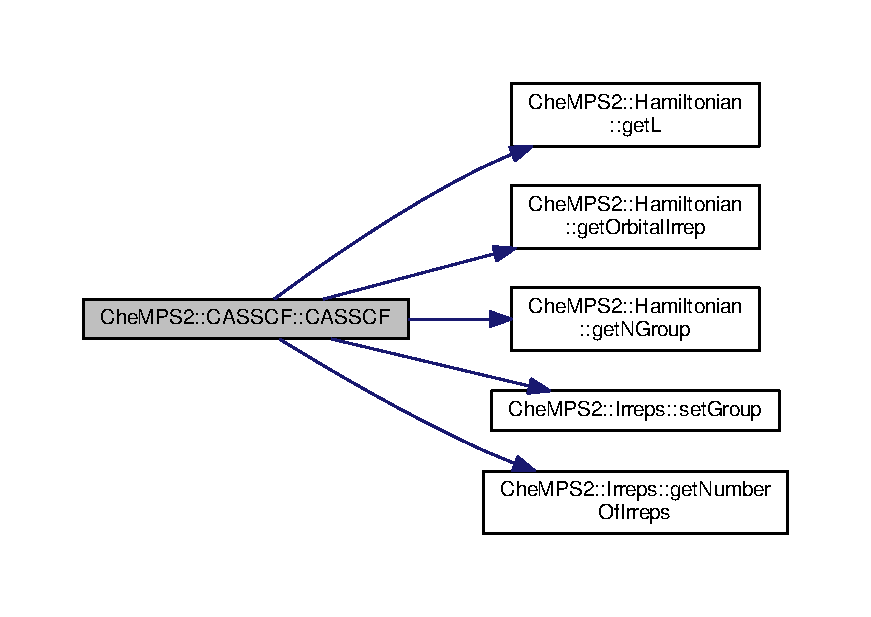
\includegraphics[width=350pt]{classCheMPS2_1_1CASSCF_aee2071ba5914ed3a6e7120e6d1656144_cgraph}
\end{center}
\end{figure}


\hypertarget{classCheMPS2_1_1CASSCF_a9c0aeea016f892a6b4a72cee8a37bd96}{\index{Che\-M\-P\-S2\-::\-C\-A\-S\-S\-C\-F@{Che\-M\-P\-S2\-::\-C\-A\-S\-S\-C\-F}!C\-A\-S\-S\-C\-F@{C\-A\-S\-S\-C\-F}}
\index{C\-A\-S\-S\-C\-F@{C\-A\-S\-S\-C\-F}!CheMPS2::CASSCF@{Che\-M\-P\-S2\-::\-C\-A\-S\-S\-C\-F}}
\paragraph[{C\-A\-S\-S\-C\-F}]{\setlength{\rightskip}{0pt plus 5cm}Che\-M\-P\-S2\-::\-C\-A\-S\-S\-C\-F\-::\-C\-A\-S\-S\-C\-F (
\begin{DoxyParamCaption}
\item[{{\bf Hamiltonian} $\ast$}]{Ham\-In, }
\item[{int $\ast$}]{D\-O\-C\-Cin, }
\item[{int $\ast$}]{S\-O\-C\-Cin}
\end{DoxyParamCaption}
)}}\label{classCheMPS2_1_1CASSCF_a9c0aeea016f892a6b4a72cee8a37bd96}


Constructor. 


\begin{DoxyParams}{Parameters}
{\em Ham\-In} & \hyperlink{classCheMPS2_1_1Hamiltonian}{Hamiltonian} containing the matrix elements of the \hyperlink{classCheMPS2_1_1Hamiltonian}{Hamiltonian} for which a \hyperlink{classCheMPS2_1_1CASSCF}{C\-A\-S\-S\-C\-F} calculation is desired \\
\hline
{\em D\-O\-C\-Cin} & Array containing the number of doubly occupied H\-F orbitals per irrep \\
\hline
{\em S\-O\-C\-Cin} & Array containing the number of singly occupied H\-F orbitals per irrep \\
\hline
\end{DoxyParams}


Definition at line 63 of file C\-A\-S\-S\-C\-F.\-cpp.



Here is the call graph for this function\-:\nopagebreak
\begin{figure}[H]
\begin{center}
\leavevmode
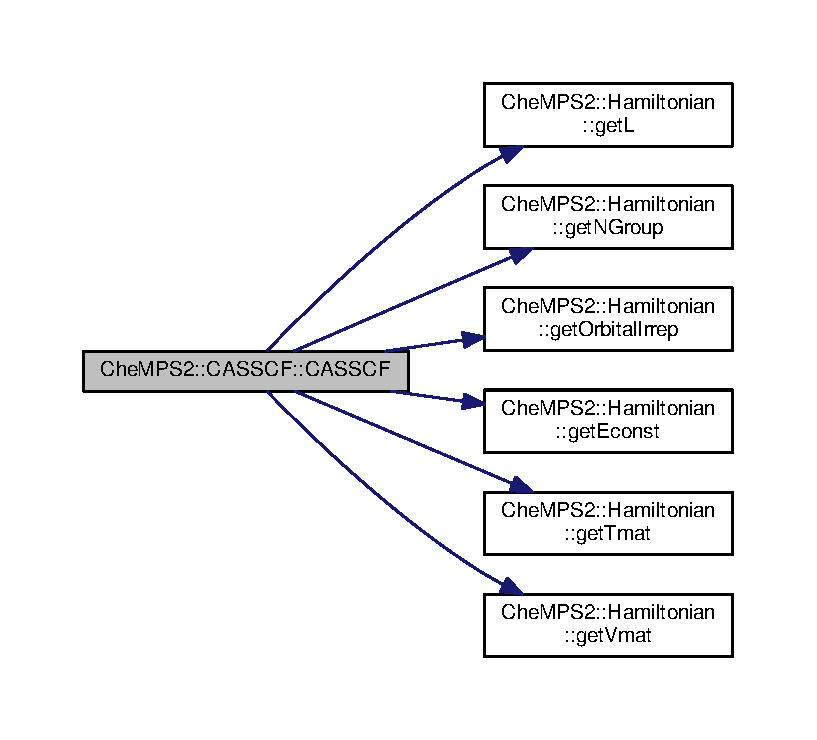
\includegraphics[width=350pt]{classCheMPS2_1_1CASSCF_a9c0aeea016f892a6b4a72cee8a37bd96_cgraph}
\end{center}
\end{figure}




\subsubsection{Member Function Documentation}
\hypertarget{classCheMPS2_1_1CASSCF_aee8753e7169f61e4804ddbc1b7e8409d}{\index{Che\-M\-P\-S2\-::\-C\-A\-S\-S\-C\-F@{Che\-M\-P\-S2\-::\-C\-A\-S\-S\-C\-F}!do\-C\-A\-S\-S\-C\-Fnewtonraphson@{do\-C\-A\-S\-S\-C\-Fnewtonraphson}}
\index{do\-C\-A\-S\-S\-C\-Fnewtonraphson@{do\-C\-A\-S\-S\-C\-Fnewtonraphson}!CheMPS2::CASSCF@{Che\-M\-P\-S2\-::\-C\-A\-S\-S\-C\-F}}
\paragraph[{do\-C\-A\-S\-S\-C\-Fnewtonraphson}]{\setlength{\rightskip}{0pt plus 5cm}double Che\-M\-P\-S2\-::\-C\-A\-S\-S\-C\-F\-::do\-C\-A\-S\-S\-C\-Fnewtonraphson (
\begin{DoxyParamCaption}
\item[{const int}]{Nelectrons, }
\item[{const int}]{Two\-S, }
\item[{const int}]{Irrep, }
\item[{{\bf Convergence\-Scheme} $\ast$}]{Opt\-Scheme, }
\item[{const int}]{root\-Num}
\end{DoxyParamCaption}
)}}\label{classCheMPS2_1_1CASSCF_aee8753e7169f61e4804ddbc1b7e8409d}


Does the state-\/specific \hyperlink{classCheMPS2_1_1CASSCF}{C\-A\-S\-S\-C\-F} cycle with the (augmented hessian) newton raphson method. 


\begin{DoxyParams}{Parameters}
{\em Nelectrons} & Total number of electrons in the system\-: occupied H\-F orbitals + active space \\
\hline
{\em Two\-S} & Twice the targeted spin \\
\hline
{\em Irrep} & Desired wave-\/function irrep \\
\hline
{\em Opt\-Scheme} & The optimization scheme to run the inner \hyperlink{classCheMPS2_1_1DMRG}{D\-M\-R\-G} loop \\
\hline
{\em root\-Num} & Denotes the targeted state in state-\/specific \hyperlink{classCheMPS2_1_1CASSCF}{C\-A\-S\-S\-C\-F}; 1 means ground state, 2 first excited state etc. \\
\hline
\end{DoxyParams}


Definition at line 36 of file C\-A\-S\-S\-C\-Fnewtonraphson.\-cpp.



Here is the call graph for this function\-:\nopagebreak
\begin{figure}[H]
\begin{center}
\leavevmode
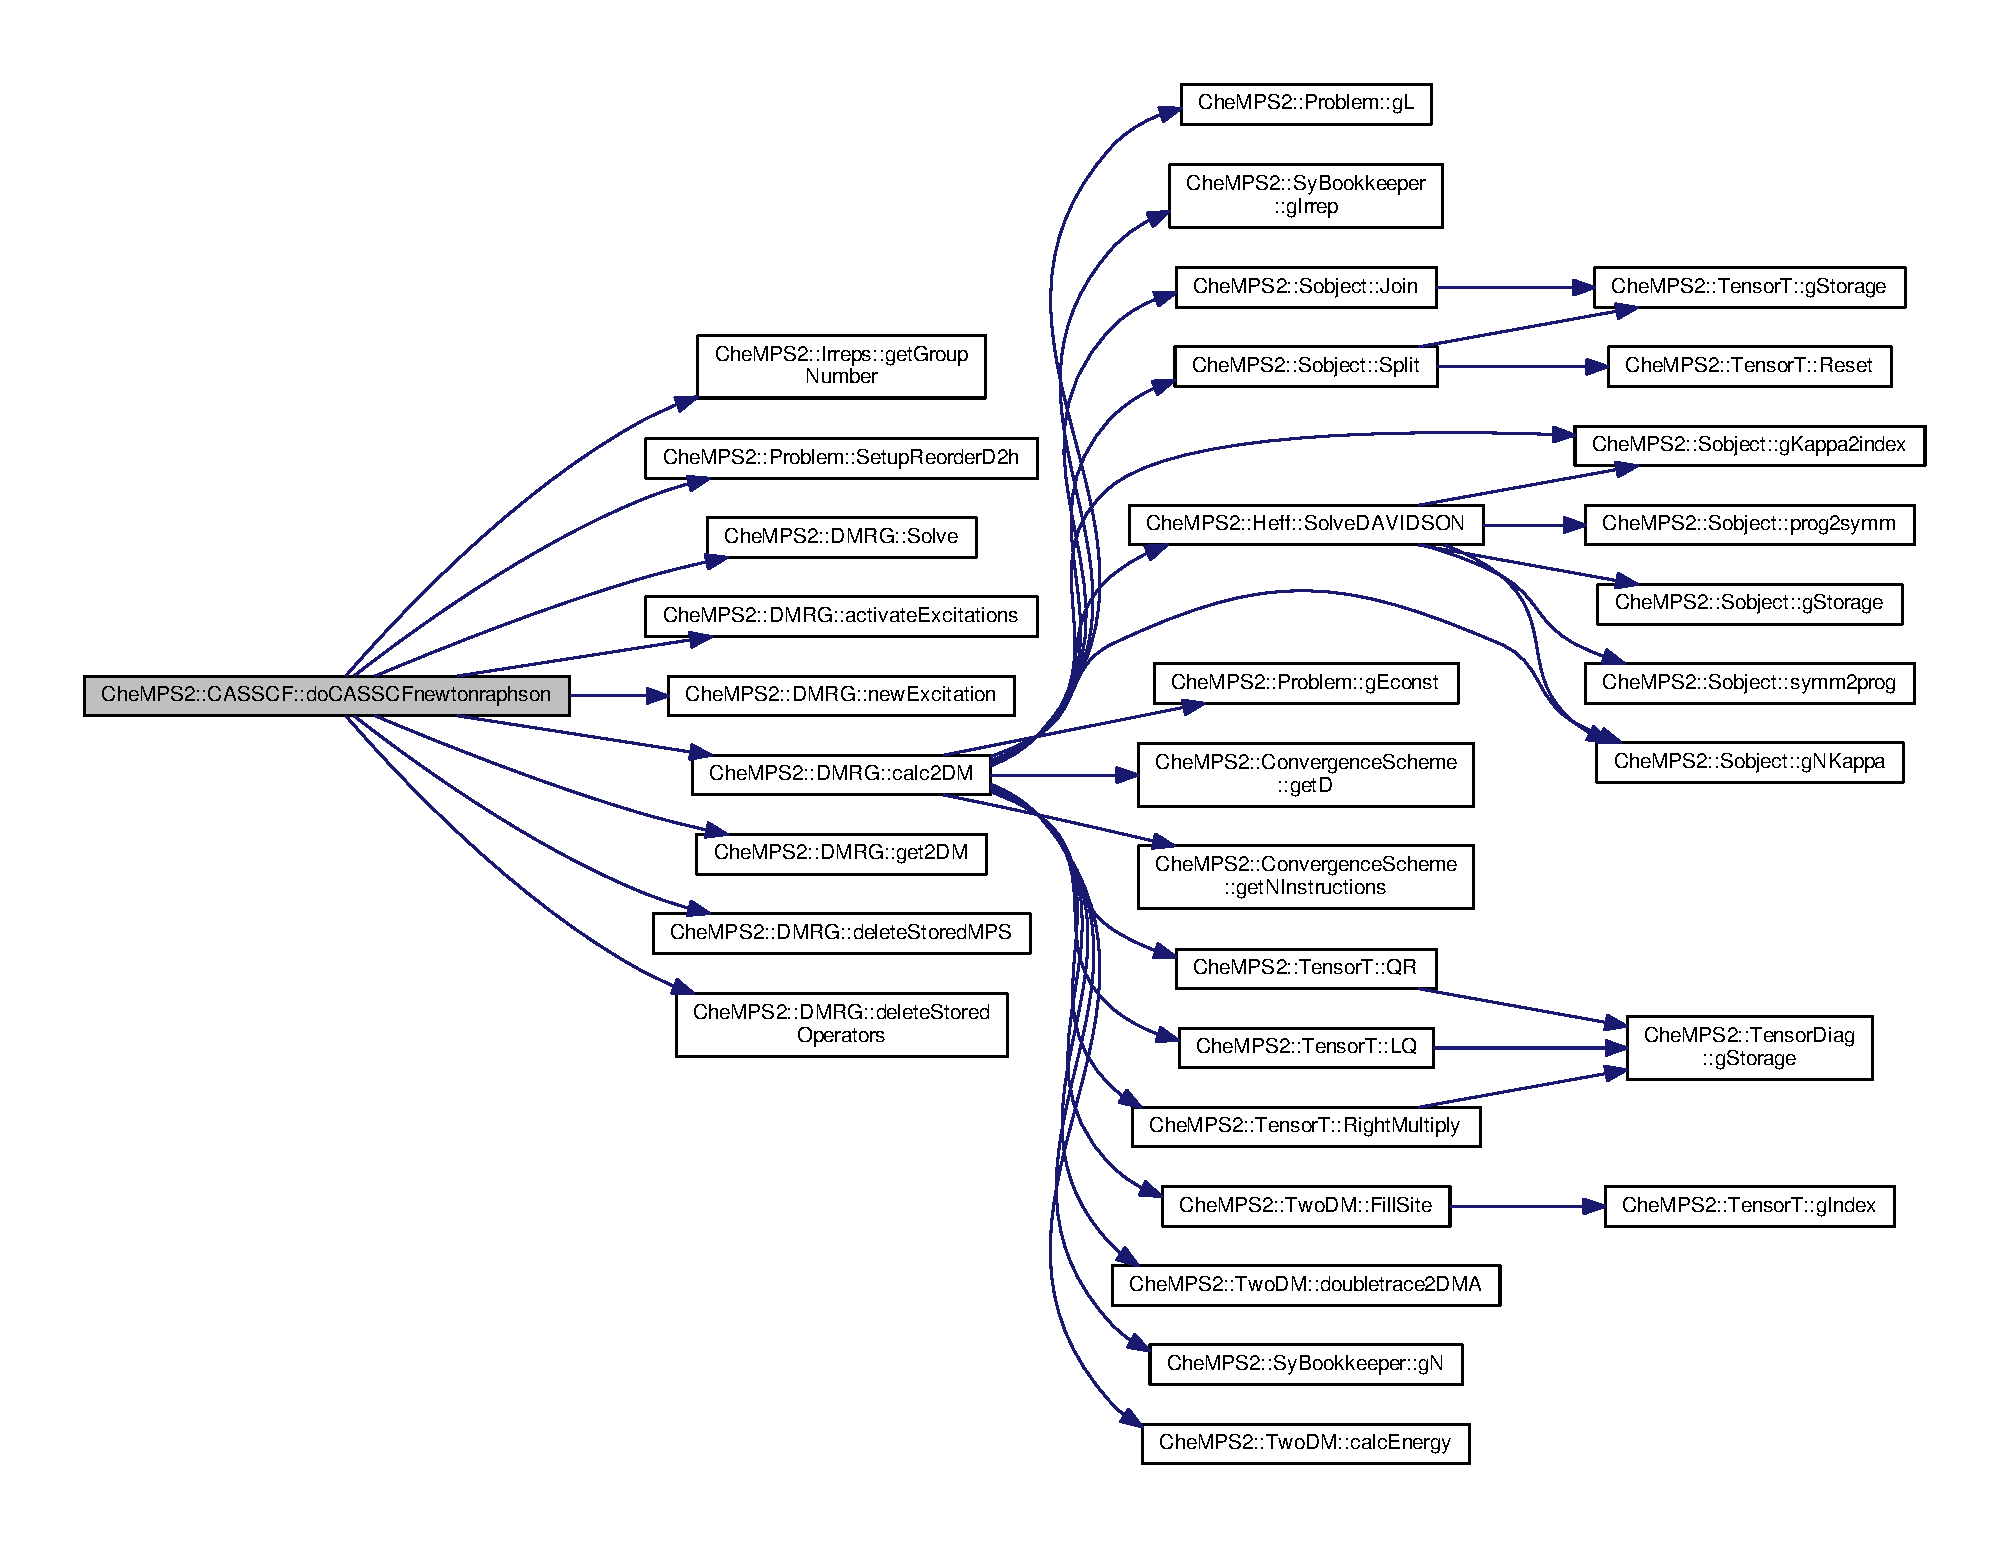
\includegraphics[width=350pt]{classCheMPS2_1_1CASSCF_aee8753e7169f61e4804ddbc1b7e8409d_cgraph}
\end{center}
\end{figure}


\hypertarget{classCheMPS2_1_1CASSCF_afba8add72828a26c426f47a790511bf1}{\index{Che\-M\-P\-S2\-::\-C\-A\-S\-S\-C\-F@{Che\-M\-P\-S2\-::\-C\-A\-S\-S\-C\-F}!get\-Number\-Of\-Irreps@{get\-Number\-Of\-Irreps}}
\index{get\-Number\-Of\-Irreps@{get\-Number\-Of\-Irreps}!CheMPS2::CASSCF@{Che\-M\-P\-S2\-::\-C\-A\-S\-S\-C\-F}}
\paragraph[{get\-Number\-Of\-Irreps}]{\setlength{\rightskip}{0pt plus 5cm}int Che\-M\-P\-S2\-::\-C\-A\-S\-S\-C\-F\-::get\-Number\-Of\-Irreps (
\begin{DoxyParamCaption}
{}
\end{DoxyParamCaption}
)}}\label{classCheMPS2_1_1CASSCF_afba8add72828a26c426f47a790511bf1}


Get the number of irreps. 

\begin{DoxyReturn}{Returns}
The number of irreps 
\end{DoxyReturn}


Definition at line 152 of file C\-A\-S\-S\-C\-F.\-cpp.

\hypertarget{classCheMPS2_1_1CASSCF_a701bdaa40881168d6b386683eaa01cea}{\index{Che\-M\-P\-S2\-::\-C\-A\-S\-S\-C\-F@{Che\-M\-P\-S2\-::\-C\-A\-S\-S\-C\-F}!setup\-Start@{setup\-Start}}
\index{setup\-Start@{setup\-Start}!CheMPS2::CASSCF@{Che\-M\-P\-S2\-::\-C\-A\-S\-S\-C\-F}}
\paragraph[{setup\-Start}]{\setlength{\rightskip}{0pt plus 5cm}void Che\-M\-P\-S2\-::\-C\-A\-S\-S\-C\-F\-::setup\-Start (
\begin{DoxyParamCaption}
\item[{int $\ast$}]{Nocc\-In, }
\item[{int $\ast$}]{N\-D\-M\-R\-G\-In, }
\item[{int $\ast$}]{Nvirt\-In}
\end{DoxyParamCaption}
)}}\label{classCheMPS2_1_1CASSCF_a701bdaa40881168d6b386683eaa01cea}


Set the start of the \hyperlink{classCheMPS2_1_1CASSCF}{C\-A\-S\-S\-C\-F} calculation. 


\begin{DoxyParams}{Parameters}
{\em Nocc\-In} & Array of length number\-Of\-Irreps containing the number of double occupied H\-F orbitals per irrep for the \hyperlink{classCheMPS2_1_1CASSCF}{C\-A\-S\-S\-C\-F} loop. \\
\hline
{\em N\-D\-M\-R\-G\-In} & Array of length number\-Of\-Irreps containing the number of active orbitals per irrep for the \hyperlink{classCheMPS2_1_1CASSCF}{C\-A\-S\-S\-C\-F} loop. \\
\hline
{\em Nvirt\-In} & Array of length number\-Of\-Irreps containing the number of empty orbitals per irrep for the \hyperlink{classCheMPS2_1_1CASSCF}{C\-A\-S\-S\-C\-F} loop. \\
\hline
\end{DoxyParams}


Definition at line 650 of file C\-A\-S\-S\-C\-F.\-cpp.



The documentation for this class was generated from the following files\-:\begin{DoxyCompactItemize}
\item 
C\-A\-S\-S\-C\-F.\-h\item 
C\-A\-S\-S\-C\-F.\-cpp\item 
C\-A\-S\-S\-C\-Fdebug.\-cpp\item 
C\-A\-S\-S\-C\-Fhamiltonianrotation.\-cpp\item 
C\-A\-S\-S\-C\-Fnewtonraphson.\-cpp\end{DoxyCompactItemize}

\hypertarget{classCheMPS2_1_1ConvergenceScheme}{\subsection{Che\-M\-P\-S2\-:\-:Convergence\-Scheme Class Reference}
\label{classCheMPS2_1_1ConvergenceScheme}\index{Che\-M\-P\-S2\-::\-Convergence\-Scheme@{Che\-M\-P\-S2\-::\-Convergence\-Scheme}}
}


{\ttfamily \#include $<$Convergence\-Scheme.\-h$>$}

\subsubsection*{Public Member Functions}
\begin{DoxyCompactItemize}
\item 
\hyperlink{classCheMPS2_1_1ConvergenceScheme_a8aa20cc325aa2c2332bec394bb05823c}{Convergence\-Scheme} (const int n\-Instructions)
\begin{DoxyCompactList}\small\item\em Constructor. \end{DoxyCompactList}\item 
\hypertarget{classCheMPS2_1_1ConvergenceScheme_af2ca92fc4ac3bbe78ae0ee252c58fab1}{\hyperlink{classCheMPS2_1_1ConvergenceScheme_af2ca92fc4ac3bbe78ae0ee252c58fab1}{$\sim$\-Convergence\-Scheme} ()}\label{classCheMPS2_1_1ConvergenceScheme_af2ca92fc4ac3bbe78ae0ee252c58fab1}

\begin{DoxyCompactList}\small\item\em Destructor. \end{DoxyCompactList}\item 
int \hyperlink{classCheMPS2_1_1ConvergenceScheme_ab8c98d5388c415c42115084c5817e1dc}{get\-N\-Instructions} ()
\begin{DoxyCompactList}\small\item\em Get the number of instructions. \end{DoxyCompactList}\item 
void \hyperlink{classCheMPS2_1_1ConvergenceScheme_a454421f377a2be63872d9199b84bad95}{set\-Instruction} (const int instruction, const int D, const double Econv, const int n\-Max, const double noise\-Prefactor)
\begin{DoxyCompactList}\small\item\em Set an instruction. \end{DoxyCompactList}\item 
int \hyperlink{classCheMPS2_1_1ConvergenceScheme_abb766295f71d3c1e3b9edc875504b317}{get\-D} (const int instruction)
\begin{DoxyCompactList}\small\item\em Get the number of renormalized states for a particular instruction. \end{DoxyCompactList}\item 
double \hyperlink{classCheMPS2_1_1ConvergenceScheme_a531e6d2a63b7fb8ad6d09bffd740687f}{get\-Econv} (const int instruction)
\begin{DoxyCompactList}\small\item\em Get the energy convergence threshold for a particular instruction. \end{DoxyCompactList}\item 
int \hyperlink{classCheMPS2_1_1ConvergenceScheme_abab59f923fab04a8def8ec6af9748df5}{get\-Max\-Sweeps} (const int instruction)
\begin{DoxyCompactList}\small\item\em Get the maximum number of sweeps for a particular instruction. \end{DoxyCompactList}\item 
double \hyperlink{classCheMPS2_1_1ConvergenceScheme_a06c60aeec22896b5018541ebcae2aeb8}{get\-Noise\-Prefactor} (const int instruction)
\begin{DoxyCompactList}\small\item\em Get the noise prefactor for a particular instruction. \end{DoxyCompactList}\end{DoxyCompactItemize}


\subsubsection{Detailed Description}
\hyperlink{classCheMPS2_1_1ConvergenceScheme}{Convergence\-Scheme} class. \begin{DoxyAuthor}{Author}
Sebastian Wouters \href{mailto:sebastianwouters@gmail.com}{\tt sebastianwouters@gmail.\-com} 
\end{DoxyAuthor}
\begin{DoxyDate}{Date}
November 7, 2013
\end{DoxyDate}
The \hyperlink{classCheMPS2_1_1ConvergenceScheme}{Convergence\-Scheme} class contains the convergence settings. This is a list of instructions, which are performed in order. Each instruction line contains the information for one particular batch of \hyperlink{classCheMPS2_1_1DMRG}{D\-M\-R\-G} sweeps\-:\par
 (1) the number of renormalized basis states to keep (D)\par
 (2) the energy convergence threshold for energy changes per left-\/ and right-\/sweep\par
 (3) the maximum number of iterations, in case the energy changes do not drop below the threshold\par
 (4) the noise prefactor f\par
 \par
 The noise level which is added to the \hyperlink{classCheMPS2_1_1Sobject}{Sobject} is the product of\par
 (1) f\par
 (2) the maximum discarded weight during the last sweep\par
 (3) a random number in the interval \mbox{[}-\/0.\-5,0.\-5\mbox{]} 

Definition at line 38 of file Convergence\-Scheme.\-h.



\subsubsection{Constructor \& Destructor Documentation}
\hypertarget{classCheMPS2_1_1ConvergenceScheme_a8aa20cc325aa2c2332bec394bb05823c}{\index{Che\-M\-P\-S2\-::\-Convergence\-Scheme@{Che\-M\-P\-S2\-::\-Convergence\-Scheme}!Convergence\-Scheme@{Convergence\-Scheme}}
\index{Convergence\-Scheme@{Convergence\-Scheme}!CheMPS2::ConvergenceScheme@{Che\-M\-P\-S2\-::\-Convergence\-Scheme}}
\paragraph[{Convergence\-Scheme}]{\setlength{\rightskip}{0pt plus 5cm}Che\-M\-P\-S2\-::\-Convergence\-Scheme\-::\-Convergence\-Scheme (
\begin{DoxyParamCaption}
\item[{const int}]{n\-Instructions}
\end{DoxyParamCaption}
)}}\label{classCheMPS2_1_1ConvergenceScheme_a8aa20cc325aa2c2332bec394bb05823c}


Constructor. 


\begin{DoxyParams}{Parameters}
{\em n\-Instructions} & the number of instructions \\
\hline
\end{DoxyParams}


Definition at line 28 of file Convergence\-Scheme.\-cpp.



\subsubsection{Member Function Documentation}
\hypertarget{classCheMPS2_1_1ConvergenceScheme_abb766295f71d3c1e3b9edc875504b317}{\index{Che\-M\-P\-S2\-::\-Convergence\-Scheme@{Che\-M\-P\-S2\-::\-Convergence\-Scheme}!get\-D@{get\-D}}
\index{get\-D@{get\-D}!CheMPS2::ConvergenceScheme@{Che\-M\-P\-S2\-::\-Convergence\-Scheme}}
\paragraph[{get\-D}]{\setlength{\rightskip}{0pt plus 5cm}int Che\-M\-P\-S2\-::\-Convergence\-Scheme\-::get\-D (
\begin{DoxyParamCaption}
\item[{const int}]{instruction}
\end{DoxyParamCaption}
)}}\label{classCheMPS2_1_1ConvergenceScheme_abb766295f71d3c1e3b9edc875504b317}


Get the number of renormalized states for a particular instruction. 


\begin{DoxyParams}{Parameters}
{\em instruction} & the number of the instruction \\
\hline
\end{DoxyParams}
\begin{DoxyReturn}{Returns}
the number of renormalized states for this instruction 
\end{DoxyReturn}


Definition at line 75 of file Convergence\-Scheme.\-cpp.



Here is the caller graph for this function\-:\nopagebreak
\begin{figure}[H]
\begin{center}
\leavevmode
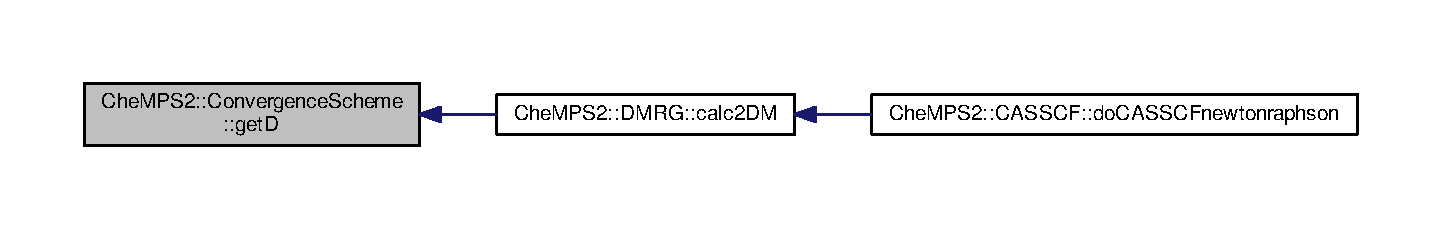
\includegraphics[width=350pt]{classCheMPS2_1_1ConvergenceScheme_abb766295f71d3c1e3b9edc875504b317_icgraph}
\end{center}
\end{figure}


\hypertarget{classCheMPS2_1_1ConvergenceScheme_a531e6d2a63b7fb8ad6d09bffd740687f}{\index{Che\-M\-P\-S2\-::\-Convergence\-Scheme@{Che\-M\-P\-S2\-::\-Convergence\-Scheme}!get\-Econv@{get\-Econv}}
\index{get\-Econv@{get\-Econv}!CheMPS2::ConvergenceScheme@{Che\-M\-P\-S2\-::\-Convergence\-Scheme}}
\paragraph[{get\-Econv}]{\setlength{\rightskip}{0pt plus 5cm}double Che\-M\-P\-S2\-::\-Convergence\-Scheme\-::get\-Econv (
\begin{DoxyParamCaption}
\item[{const int}]{instruction}
\end{DoxyParamCaption}
)}}\label{classCheMPS2_1_1ConvergenceScheme_a531e6d2a63b7fb8ad6d09bffd740687f}


Get the energy convergence threshold for a particular instruction. 


\begin{DoxyParams}{Parameters}
{\em instruction} & the number of the instruction \\
\hline
\end{DoxyParams}
\begin{DoxyReturn}{Returns}
the energy convergence threshold for this instruction 
\end{DoxyReturn}


Definition at line 77 of file Convergence\-Scheme.\-cpp.

\hypertarget{classCheMPS2_1_1ConvergenceScheme_abab59f923fab04a8def8ec6af9748df5}{\index{Che\-M\-P\-S2\-::\-Convergence\-Scheme@{Che\-M\-P\-S2\-::\-Convergence\-Scheme}!get\-Max\-Sweeps@{get\-Max\-Sweeps}}
\index{get\-Max\-Sweeps@{get\-Max\-Sweeps}!CheMPS2::ConvergenceScheme@{Che\-M\-P\-S2\-::\-Convergence\-Scheme}}
\paragraph[{get\-Max\-Sweeps}]{\setlength{\rightskip}{0pt plus 5cm}int Che\-M\-P\-S2\-::\-Convergence\-Scheme\-::get\-Max\-Sweeps (
\begin{DoxyParamCaption}
\item[{const int}]{instruction}
\end{DoxyParamCaption}
)}}\label{classCheMPS2_1_1ConvergenceScheme_abab59f923fab04a8def8ec6af9748df5}


Get the maximum number of sweeps for a particular instruction. 


\begin{DoxyParams}{Parameters}
{\em instruction} & the number of the instruction \\
\hline
\end{DoxyParams}
\begin{DoxyReturn}{Returns}
the maximum number of sweeps for this instruction 
\end{DoxyReturn}


Definition at line 79 of file Convergence\-Scheme.\-cpp.

\hypertarget{classCheMPS2_1_1ConvergenceScheme_ab8c98d5388c415c42115084c5817e1dc}{\index{Che\-M\-P\-S2\-::\-Convergence\-Scheme@{Che\-M\-P\-S2\-::\-Convergence\-Scheme}!get\-N\-Instructions@{get\-N\-Instructions}}
\index{get\-N\-Instructions@{get\-N\-Instructions}!CheMPS2::ConvergenceScheme@{Che\-M\-P\-S2\-::\-Convergence\-Scheme}}
\paragraph[{get\-N\-Instructions}]{\setlength{\rightskip}{0pt plus 5cm}int Che\-M\-P\-S2\-::\-Convergence\-Scheme\-::get\-N\-Instructions (
\begin{DoxyParamCaption}
{}
\end{DoxyParamCaption}
)}}\label{classCheMPS2_1_1ConvergenceScheme_ab8c98d5388c415c42115084c5817e1dc}


Get the number of instructions. 

return the number of instructions to converge the \hyperlink{classCheMPS2_1_1DMRG}{D\-M\-R\-G} calculation 

Definition at line 52 of file Convergence\-Scheme.\-cpp.



Here is the caller graph for this function\-:\nopagebreak
\begin{figure}[H]
\begin{center}
\leavevmode
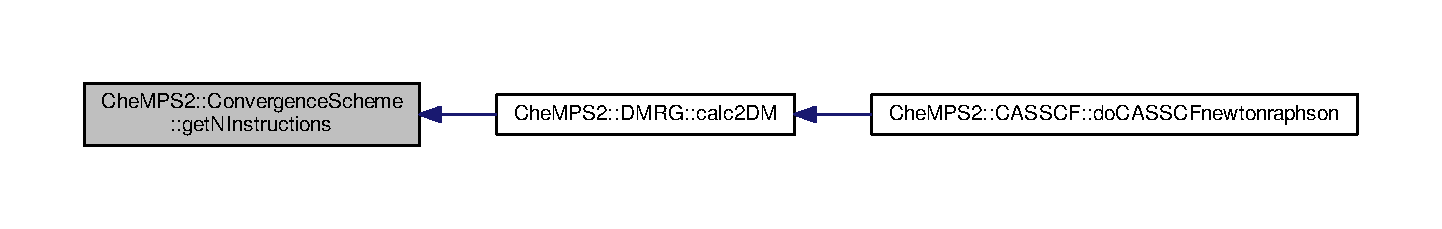
\includegraphics[width=350pt]{classCheMPS2_1_1ConvergenceScheme_ab8c98d5388c415c42115084c5817e1dc_icgraph}
\end{center}
\end{figure}


\hypertarget{classCheMPS2_1_1ConvergenceScheme_a06c60aeec22896b5018541ebcae2aeb8}{\index{Che\-M\-P\-S2\-::\-Convergence\-Scheme@{Che\-M\-P\-S2\-::\-Convergence\-Scheme}!get\-Noise\-Prefactor@{get\-Noise\-Prefactor}}
\index{get\-Noise\-Prefactor@{get\-Noise\-Prefactor}!CheMPS2::ConvergenceScheme@{Che\-M\-P\-S2\-::\-Convergence\-Scheme}}
\paragraph[{get\-Noise\-Prefactor}]{\setlength{\rightskip}{0pt plus 5cm}double Che\-M\-P\-S2\-::\-Convergence\-Scheme\-::get\-Noise\-Prefactor (
\begin{DoxyParamCaption}
\item[{const int}]{instruction}
\end{DoxyParamCaption}
)}}\label{classCheMPS2_1_1ConvergenceScheme_a06c60aeec22896b5018541ebcae2aeb8}


Get the noise prefactor for a particular instruction. 


\begin{DoxyParams}{Parameters}
{\em instruction} & the number of the instruction \\
\hline
\end{DoxyParams}
\begin{DoxyReturn}{Returns}
the noise prefactor for this instruction 
\end{DoxyReturn}


Definition at line 81 of file Convergence\-Scheme.\-cpp.

\hypertarget{classCheMPS2_1_1ConvergenceScheme_a454421f377a2be63872d9199b84bad95}{\index{Che\-M\-P\-S2\-::\-Convergence\-Scheme@{Che\-M\-P\-S2\-::\-Convergence\-Scheme}!set\-Instruction@{set\-Instruction}}
\index{set\-Instruction@{set\-Instruction}!CheMPS2::ConvergenceScheme@{Che\-M\-P\-S2\-::\-Convergence\-Scheme}}
\paragraph[{set\-Instruction}]{\setlength{\rightskip}{0pt plus 5cm}void Che\-M\-P\-S2\-::\-Convergence\-Scheme\-::set\-Instruction (
\begin{DoxyParamCaption}
\item[{const int}]{instruction, }
\item[{const int}]{D, }
\item[{const double}]{Econv, }
\item[{const int}]{n\-Max, }
\item[{const double}]{noise\-Prefactor}
\end{DoxyParamCaption}
)}}\label{classCheMPS2_1_1ConvergenceScheme_a454421f377a2be63872d9199b84bad95}


Set an instruction. 


\begin{DoxyParams}{Parameters}
{\em instruction} & the number of the instruction \\
\hline
{\em D} & the number of renormalized states for that instruction \\
\hline
{\em Econv} & the energy convergence threshold for that instruction \\
\hline
{\em n\-Max} & the max. number of sweeps for that instruction \\
\hline
{\em noise\-Prefactor} & the noise prefactor for that instruction \\
\hline
\end{DoxyParams}


Definition at line 54 of file Convergence\-Scheme.\-cpp.



The documentation for this class was generated from the following files\-:\begin{DoxyCompactItemize}
\item 
Convergence\-Scheme.\-h\item 
Convergence\-Scheme.\-cpp\end{DoxyCompactItemize}

\hypertarget{classCheMPS2_1_1DMRG}{\subsection{Che\-M\-P\-S2\-:\-:D\-M\-R\-G Class Reference}
\label{classCheMPS2_1_1DMRG}\index{Che\-M\-P\-S2\-::\-D\-M\-R\-G@{Che\-M\-P\-S2\-::\-D\-M\-R\-G}}
}


{\ttfamily \#include $<$D\-M\-R\-G.\-h$>$}

\subsubsection*{Public Member Functions}
\begin{DoxyCompactItemize}
\item 
\hyperlink{classCheMPS2_1_1DMRG_af75174435718b0b533712fbeb6568c71}{D\-M\-R\-G} (\hyperlink{classCheMPS2_1_1Problem}{Problem} $\ast$Probin, \hyperlink{classCheMPS2_1_1ConvergenceScheme}{Convergence\-Scheme} $\ast$Opt\-Scheme\-In)
\begin{DoxyCompactList}\small\item\em Constructor. \end{DoxyCompactList}\item 
\hypertarget{classCheMPS2_1_1DMRG_abe701c20aeb97b48c237bed694d185b5}{\hyperlink{classCheMPS2_1_1DMRG_abe701c20aeb97b48c237bed694d185b5}{$\sim$\-D\-M\-R\-G} ()}\label{classCheMPS2_1_1DMRG_abe701c20aeb97b48c237bed694d185b5}

\begin{DoxyCompactList}\small\item\em Destructor. \end{DoxyCompactList}\item 
double \hyperlink{classCheMPS2_1_1DMRG_ab6d80dde8b71171ee969a6b7b86193d2}{Solve} ()
\begin{DoxyCompactList}\small\item\em Solver. \end{DoxyCompactList}\item 
\hypertarget{classCheMPS2_1_1DMRG_a35db8f58be5130548d5998ccbda4d37e}{void \hyperlink{classCheMPS2_1_1DMRG_a35db8f58be5130548d5998ccbda4d37e}{calc2\-D\-M} ()}\label{classCheMPS2_1_1DMRG_a35db8f58be5130548d5998ccbda4d37e}

\begin{DoxyCompactList}\small\item\em Calculate the 2\-D\-M. Note that the \hyperlink{classCheMPS2_1_1DMRG}{D\-M\-R\-G} class cannot be used for further updates anymore !!! \end{DoxyCompactList}\item 
\hypertarget{classCheMPS2_1_1DMRG_aa08c71dab6543ef820d13528fc354bcd}{\hyperlink{classCheMPS2_1_1TwoDM}{Two\-D\-M} $\ast$ \hyperlink{classCheMPS2_1_1DMRG_aa08c71dab6543ef820d13528fc354bcd}{get2\-D\-M} ()}\label{classCheMPS2_1_1DMRG_aa08c71dab6543ef820d13528fc354bcd}

\begin{DoxyCompactList}\small\item\em Get the pointer to the 2\-D\-M. \end{DoxyCompactList}\item 
double \hyperlink{classCheMPS2_1_1DMRG_aadcaff5f067d6625ac69237cee0ee92e}{get\-Specific\-Coefficient} (int $\ast$coeff)
\begin{DoxyCompactList}\small\item\em Get a specific F\-C\-I coefficient. coeff contains the occupation numbers of the L orbitals. It is assumed that the number of unpaired electrons equals twice the total targeted spin. \end{DoxyCompactList}\item 
\hypertarget{classCheMPS2_1_1DMRG_a0f4e487c40f522846288fe1b3d55e66c}{void \hyperlink{classCheMPS2_1_1DMRG_a0f4e487c40f522846288fe1b3d55e66c}{delete\-Stored\-M\-P\-S} ()}\label{classCheMPS2_1_1DMRG_a0f4e487c40f522846288fe1b3d55e66c}

\begin{DoxyCompactList}\small\item\em Call \char`\"{}rm Che\-M\-P\-S2\-\_\-\-M\-P\-S$\ast$.\-h5\char`\"{}. \end{DoxyCompactList}\item 
\hypertarget{classCheMPS2_1_1DMRG_a2254cc31b5d9497694ea2229226b7bd6}{void \hyperlink{classCheMPS2_1_1DMRG_a2254cc31b5d9497694ea2229226b7bd6}{delete\-Stored\-Operators} ()}\label{classCheMPS2_1_1DMRG_a2254cc31b5d9497694ea2229226b7bd6}

\begin{DoxyCompactList}\small\item\em Call \char`\"{}rm + local\-Tmp\-Path + Che\-M\-P\-S2\-\_\- + R\-Nstorage + $\ast$.\-h5\char`\"{}. \end{DoxyCompactList}\item 
void \hyperlink{classCheMPS2_1_1DMRG_ab442cbc43e2e5d877660859578849133}{activate\-Excitations} (const int max\-Exc\-In)
\begin{DoxyCompactList}\small\item\em Activate the necessary storage and machinery to handle excitations. \end{DoxyCompactList}\item 
void \hyperlink{classCheMPS2_1_1DMRG_acfb3123c72e3503f2d6c77dcf9eb141a}{new\-Excitation} (const double Eshift\-In)
\begin{DoxyCompactList}\small\item\em Push back current calculation and set everything up to calculate a (new) excitation. \end{DoxyCompactList}\item 
\hypertarget{classCheMPS2_1_1DMRG_a6c8741ce96ac0e806a8ddc6c3623d904}{void \hyperlink{classCheMPS2_1_1DMRG_a6c8741ce96ac0e806a8ddc6c3623d904}{Print\-License} ()}\label{classCheMPS2_1_1DMRG_a6c8741ce96ac0e806a8ddc6c3623d904}

\begin{DoxyCompactList}\small\item\em Print the license. \end{DoxyCompactList}\end{DoxyCompactItemize}


\subsubsection{Detailed Description}
\hyperlink{classCheMPS2_1_1DMRG}{D\-M\-R\-G} class. \begin{DoxyAuthor}{Author}
Sebastian Wouters \href{mailto:sebastianwouters@gmail.com}{\tt sebastianwouters@gmail.\-com} 
\end{DoxyAuthor}
\begin{DoxyDate}{Date}
July 31, 2013
\end{DoxyDate}
The \hyperlink{classCheMPS2_1_1DMRG}{D\-M\-R\-G} class solves the \hyperlink{classCheMPS2_1_1Problem}{Problem} with its given parameters. A fully S\-U(2) symmetric M\-P\-S wavefunction is variationally optimized in a two-\/site sweep algorithm. When the solution has been reached, the converged energy and spin contracted 2\-D\-Ms can be accessed. 

Definition at line 53 of file D\-M\-R\-G.\-h.



\subsubsection{Constructor \& Destructor Documentation}
\hypertarget{classCheMPS2_1_1DMRG_af75174435718b0b533712fbeb6568c71}{\index{Che\-M\-P\-S2\-::\-D\-M\-R\-G@{Che\-M\-P\-S2\-::\-D\-M\-R\-G}!D\-M\-R\-G@{D\-M\-R\-G}}
\index{D\-M\-R\-G@{D\-M\-R\-G}!CheMPS2::DMRG@{Che\-M\-P\-S2\-::\-D\-M\-R\-G}}
\paragraph[{D\-M\-R\-G}]{\setlength{\rightskip}{0pt plus 5cm}Che\-M\-P\-S2\-::\-D\-M\-R\-G\-::\-D\-M\-R\-G (
\begin{DoxyParamCaption}
\item[{{\bf Problem} $\ast$}]{Probin, }
\item[{{\bf Convergence\-Scheme} $\ast$}]{Opt\-Scheme\-In}
\end{DoxyParamCaption}
)}}\label{classCheMPS2_1_1DMRG_af75174435718b0b533712fbeb6568c71}


Constructor. 


\begin{DoxyParams}{Parameters}
{\em Probin} & The problem to be solved \\
\hline
{\em Opt\-Scheme\-In} & The optimization scheme for the \hyperlink{classCheMPS2_1_1DMRG}{D\-M\-R\-G} sweeps \\
\hline
\end{DoxyParams}


Definition at line 33 of file D\-M\-R\-G.\-cpp.



Here is the call graph for this function\-:\nopagebreak
\begin{figure}[H]
\begin{center}
\leavevmode
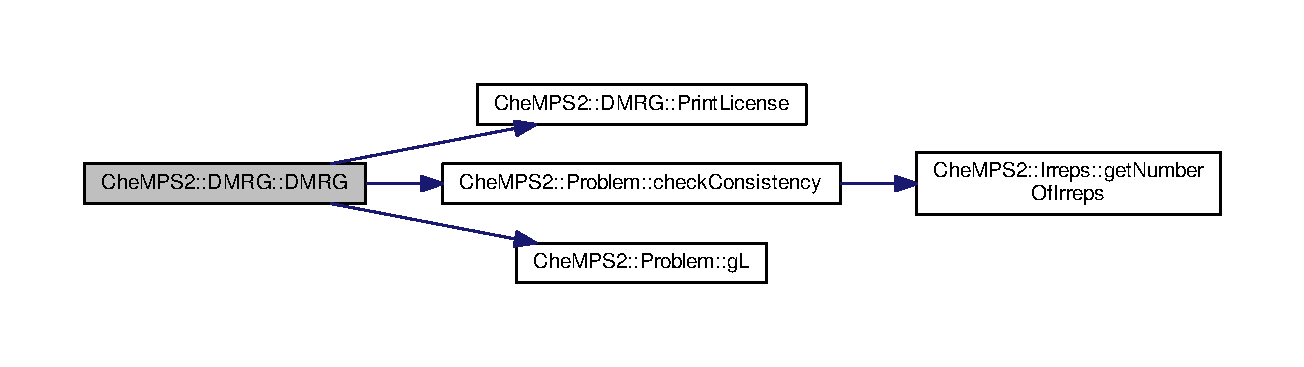
\includegraphics[width=350pt]{classCheMPS2_1_1DMRG_af75174435718b0b533712fbeb6568c71_cgraph}
\end{center}
\end{figure}




\subsubsection{Member Function Documentation}
\hypertarget{classCheMPS2_1_1DMRG_ab442cbc43e2e5d877660859578849133}{\index{Che\-M\-P\-S2\-::\-D\-M\-R\-G@{Che\-M\-P\-S2\-::\-D\-M\-R\-G}!activate\-Excitations@{activate\-Excitations}}
\index{activate\-Excitations@{activate\-Excitations}!CheMPS2::DMRG@{Che\-M\-P\-S2\-::\-D\-M\-R\-G}}
\paragraph[{activate\-Excitations}]{\setlength{\rightskip}{0pt plus 5cm}void Che\-M\-P\-S2\-::\-D\-M\-R\-G\-::activate\-Excitations (
\begin{DoxyParamCaption}
\item[{const int}]{max\-Exc\-In}
\end{DoxyParamCaption}
)}}\label{classCheMPS2_1_1DMRG_ab442cbc43e2e5d877660859578849133}


Activate the necessary storage and machinery to handle excitations. 


\begin{DoxyParams}{Parameters}
{\em max\-Exc\-In} & The max. number of excitations desired \\
\hline
\end{DoxyParams}


Definition at line 298 of file D\-M\-R\-G.\-cpp.



Here is the caller graph for this function\-:\nopagebreak
\begin{figure}[H]
\begin{center}
\leavevmode
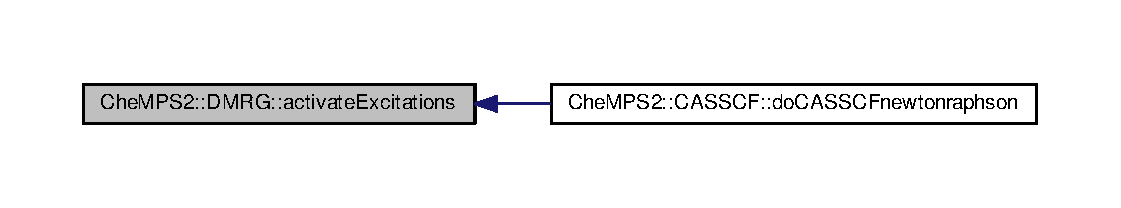
\includegraphics[width=350pt]{classCheMPS2_1_1DMRG_ab442cbc43e2e5d877660859578849133_icgraph}
\end{center}
\end{figure}


\hypertarget{classCheMPS2_1_1DMRG_aadcaff5f067d6625ac69237cee0ee92e}{\index{Che\-M\-P\-S2\-::\-D\-M\-R\-G@{Che\-M\-P\-S2\-::\-D\-M\-R\-G}!get\-Specific\-Coefficient@{get\-Specific\-Coefficient}}
\index{get\-Specific\-Coefficient@{get\-Specific\-Coefficient}!CheMPS2::DMRG@{Che\-M\-P\-S2\-::\-D\-M\-R\-G}}
\paragraph[{get\-Specific\-Coefficient}]{\setlength{\rightskip}{0pt plus 5cm}double Che\-M\-P\-S2\-::\-D\-M\-R\-G\-::get\-Specific\-Coefficient (
\begin{DoxyParamCaption}
\item[{int $\ast$}]{coeff}
\end{DoxyParamCaption}
)}}\label{classCheMPS2_1_1DMRG_aadcaff5f067d6625ac69237cee0ee92e}


Get a specific F\-C\-I coefficient. coeff contains the occupation numbers of the L orbitals. It is assumed that the number of unpaired electrons equals twice the total targeted spin. 


\begin{DoxyParams}{Parameters}
{\em coeff} & Array containing the occupation numbers of the L \hyperlink{classCheMPS2_1_1Hamiltonian}{Hamiltonian} orbitals. \\
\hline
\end{DoxyParams}
\begin{DoxyReturn}{Returns}
the desired F\-C\-I coefficient 
\end{DoxyReturn}


Definition at line 96 of file D\-M\-R\-Gtechnics.\-cpp.

\hypertarget{classCheMPS2_1_1DMRG_acfb3123c72e3503f2d6c77dcf9eb141a}{\index{Che\-M\-P\-S2\-::\-D\-M\-R\-G@{Che\-M\-P\-S2\-::\-D\-M\-R\-G}!new\-Excitation@{new\-Excitation}}
\index{new\-Excitation@{new\-Excitation}!CheMPS2::DMRG@{Che\-M\-P\-S2\-::\-D\-M\-R\-G}}
\paragraph[{new\-Excitation}]{\setlength{\rightskip}{0pt plus 5cm}void Che\-M\-P\-S2\-::\-D\-M\-R\-G\-::new\-Excitation (
\begin{DoxyParamCaption}
\item[{const double}]{Eshift\-In}
\end{DoxyParamCaption}
)}}\label{classCheMPS2_1_1DMRG_acfb3123c72e3503f2d6c77dcf9eb141a}


Push back current calculation and set everything up to calculate a (new) excitation. 


\begin{DoxyParams}{Parameters}
{\em Eshift\-In} & To the \hyperlink{classCheMPS2_1_1Hamiltonian}{Hamiltonian}, a level shift is introduced to exclude the previously calculated M\-P\-S\-: Hnew = Hold + Eshift\-In $\ast$ $|$ prev$>$ $<$prev$|$ \\
\hline
\end{DoxyParams}


Definition at line 309 of file D\-M\-R\-G.\-cpp.



Here is the caller graph for this function\-:\nopagebreak
\begin{figure}[H]
\begin{center}
\leavevmode
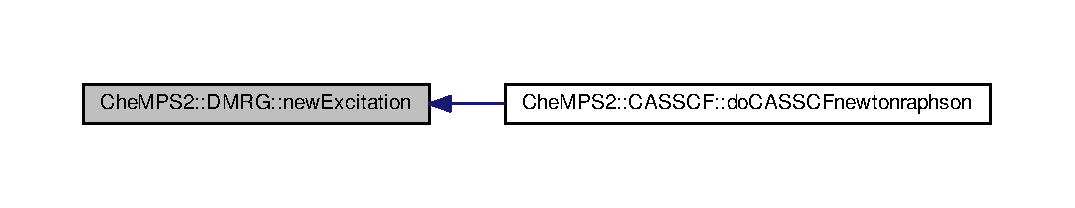
\includegraphics[width=350pt]{classCheMPS2_1_1DMRG_acfb3123c72e3503f2d6c77dcf9eb141a_icgraph}
\end{center}
\end{figure}


\hypertarget{classCheMPS2_1_1DMRG_ab6d80dde8b71171ee969a6b7b86193d2}{\index{Che\-M\-P\-S2\-::\-D\-M\-R\-G@{Che\-M\-P\-S2\-::\-D\-M\-R\-G}!Solve@{Solve}}
\index{Solve@{Solve}!CheMPS2::DMRG@{Che\-M\-P\-S2\-::\-D\-M\-R\-G}}
\paragraph[{Solve}]{\setlength{\rightskip}{0pt plus 5cm}double Che\-M\-P\-S2\-::\-D\-M\-R\-G\-::\-Solve (
\begin{DoxyParamCaption}
{}
\end{DoxyParamCaption}
)}}\label{classCheMPS2_1_1DMRG_ab6d80dde8b71171ee969a6b7b86193d2}


Solver. 

\begin{DoxyReturn}{Returns}
The min. energy encountered so far during the sweeps. 
\end{DoxyReturn}


Definition at line 157 of file D\-M\-R\-G.\-cpp.



Here is the caller graph for this function\-:\nopagebreak
\begin{figure}[H]
\begin{center}
\leavevmode
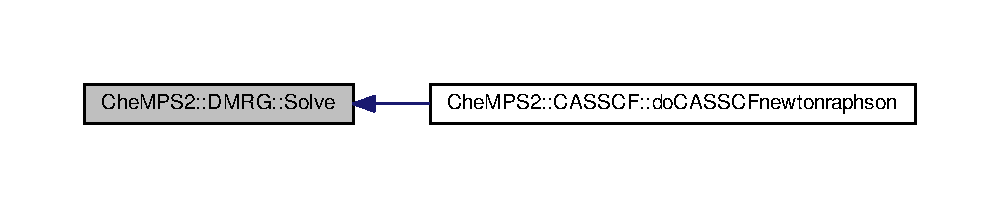
\includegraphics[width=350pt]{classCheMPS2_1_1DMRG_ab6d80dde8b71171ee969a6b7b86193d2_icgraph}
\end{center}
\end{figure}




The documentation for this class was generated from the following files\-:\begin{DoxyCompactItemize}
\item 
D\-M\-R\-G.\-h\item 
D\-M\-R\-G.\-cpp\item 
D\-M\-R\-Gmpsio.\-cpp\item 
D\-M\-R\-Goperators.\-cpp\item 
D\-M\-R\-Gtechnics.\-cpp\item 
Print\-License.\-cpp\end{DoxyCompactItemize}

\hypertarget{classCheMPS2_1_1FourIndex}{\subsection{Che\-M\-P\-S2\-:\-:Four\-Index Class Reference}
\label{classCheMPS2_1_1FourIndex}\index{Che\-M\-P\-S2\-::\-Four\-Index@{Che\-M\-P\-S2\-::\-Four\-Index}}
}


{\ttfamily \#include $<$Four\-Index.\-h$>$}

\subsubsection*{Public Member Functions}
\begin{DoxyCompactItemize}
\item 
\hyperlink{classCheMPS2_1_1FourIndex_a552ebf0c200713acdd4ce8b5222bc6ac}{Four\-Index} (const int n\-Group, const int $\ast$Irrep\-Sizes)
\begin{DoxyCompactList}\small\item\em Constructor. \end{DoxyCompactList}\item 
\hypertarget{classCheMPS2_1_1FourIndex_a4988b7745b0ec4d5f86c4af89ba20430}{virtual \hyperlink{classCheMPS2_1_1FourIndex_a4988b7745b0ec4d5f86c4af89ba20430}{$\sim$\-Four\-Index} ()}\label{classCheMPS2_1_1FourIndex_a4988b7745b0ec4d5f86c4af89ba20430}

\begin{DoxyCompactList}\small\item\em Destructor. \end{DoxyCompactList}\item 
void \hyperlink{classCheMPS2_1_1FourIndex_a8733c4fd0064bcd845786157f7d9b26f}{set} (const int irrep\-\_\-i, const int irrep\-\_\-j, const int irrep\-\_\-k, const int irrep\-\_\-l, const int i, const int j, const int k, const int l, const double val)
\begin{DoxyCompactList}\small\item\em Set an element. \end{DoxyCompactList}\item 
void \hyperlink{classCheMPS2_1_1FourIndex_a48e9e1b0939679da974e35c26281ba87}{add} (const int irrep\-\_\-i, const int irrep\-\_\-j, const int irrep\-\_\-k, const int irrep\-\_\-l, const int i, const int j, const int k, const int l, const double val)
\begin{DoxyCompactList}\small\item\em Add a double to an element. \end{DoxyCompactList}\item 
double \hyperlink{classCheMPS2_1_1FourIndex_ae93c264cbb81e7d39db778a129dc7ca1}{get} (const int irrep\-\_\-i, const int irrep\-\_\-j, const int irrep\-\_\-k, const int irrep\-\_\-l, const int i, const int j, const int k, const int l) const 
\begin{DoxyCompactList}\small\item\em Get an element. \end{DoxyCompactList}\item 
void \hyperlink{classCheMPS2_1_1FourIndex_a7d434479fe129f2c094c59f8a130361d}{save} (const std\-::string name) const 
\begin{DoxyCompactList}\small\item\em Save the \hyperlink{classCheMPS2_1_1FourIndex}{Four\-Index} object. \end{DoxyCompactList}\item 
void \hyperlink{classCheMPS2_1_1FourIndex_a557d6a17fa93c708a94fa5924626c405}{read} (const std\-::string name)
\begin{DoxyCompactList}\small\item\em Load the \hyperlink{classCheMPS2_1_1FourIndex}{Four\-Index} object. \end{DoxyCompactList}\end{DoxyCompactItemize}


\subsubsection{Detailed Description}
\hyperlink{classCheMPS2_1_1FourIndex}{Four\-Index} class. \begin{DoxyAuthor}{Author}
Sebastian Wouters \href{mailto:sebastianwouters@gmail.com}{\tt sebastianwouters@gmail.\-com} 
\end{DoxyAuthor}
\begin{DoxyDate}{Date}
February 8, 2013
\end{DoxyDate}
Container class for four-\/index tensors with Abelian point group symmetry (real character table; see \hyperlink{Irreps_8h_source}{Irreps.\-h})\-: 2\-D\-Ms and 2-\/particle matrix elements. The four-\/index tensor element V\-\_\-ijkl has 8-\/fold permutation symmetry and is only nonzero when I\-\_\-i x I\-\_\-j = I\-\_\-k x I\-\_\-l. To clarify the convention, the potential energy is given\-: \par
 $\frac{1}{2} \sum\limits_{ijkl\sigma\tau} V_{ijkl} \delta_{I_i \otimes I_j \otimes I_k \otimes I_l, I_{trivial}} \hat{a}_{i \sigma}^{\dagger} \hat{a}_{j \tau}^{\dagger} \hat{a}_{l \tau} \hat{a}_{k \sigma} $.\par
 Hence $ V_{ijkl} = ( ij \mid V \mid kl ) $ in physics notation, i.\-e. with i and k the same integration coordinate for the electron repulsion integrals. 

Definition at line 34 of file Four\-Index.\-h.



\subsubsection{Constructor \& Destructor Documentation}
\hypertarget{classCheMPS2_1_1FourIndex_a552ebf0c200713acdd4ce8b5222bc6ac}{\index{Che\-M\-P\-S2\-::\-Four\-Index@{Che\-M\-P\-S2\-::\-Four\-Index}!Four\-Index@{Four\-Index}}
\index{Four\-Index@{Four\-Index}!CheMPS2::FourIndex@{Che\-M\-P\-S2\-::\-Four\-Index}}
\paragraph[{Four\-Index}]{\setlength{\rightskip}{0pt plus 5cm}Che\-M\-P\-S2\-::\-Four\-Index\-::\-Four\-Index (
\begin{DoxyParamCaption}
\item[{const int}]{n\-Group, }
\item[{const int $\ast$}]{Irrep\-Sizes}
\end{DoxyParamCaption}
)}}\label{classCheMPS2_1_1FourIndex_a552ebf0c200713acdd4ce8b5222bc6ac}


Constructor. 


\begin{DoxyParams}{Parameters}
{\em n\-Group} & The symmetry group number (see \hyperlink{Irreps_8h_source}{Irreps.\-h}) \\
\hline
{\em Irrep\-Sizes} & Array with length the number of irreps of the specified group, containing the number of orbitals of that irrep \\
\hline
\end{DoxyParams}


Definition at line 31 of file Four\-Index.\-cpp.



\subsubsection{Member Function Documentation}
\hypertarget{classCheMPS2_1_1FourIndex_a48e9e1b0939679da974e35c26281ba87}{\index{Che\-M\-P\-S2\-::\-Four\-Index@{Che\-M\-P\-S2\-::\-Four\-Index}!add@{add}}
\index{add@{add}!CheMPS2::FourIndex@{Che\-M\-P\-S2\-::\-Four\-Index}}
\paragraph[{add}]{\setlength{\rightskip}{0pt plus 5cm}void Che\-M\-P\-S2\-::\-Four\-Index\-::add (
\begin{DoxyParamCaption}
\item[{const int}]{irrep\-\_\-i, }
\item[{const int}]{irrep\-\_\-j, }
\item[{const int}]{irrep\-\_\-k, }
\item[{const int}]{irrep\-\_\-l, }
\item[{const int}]{i, }
\item[{const int}]{j, }
\item[{const int}]{k, }
\item[{const int}]{l, }
\item[{const double}]{val}
\end{DoxyParamCaption}
)}}\label{classCheMPS2_1_1FourIndex_a48e9e1b0939679da974e35c26281ba87}


Add a double to an element. 


\begin{DoxyParams}{Parameters}
{\em irrep\-\_\-i} & The irrep number of the first orbital (see \hyperlink{Irreps_8h_source}{Irreps.\-h}) \\
\hline
{\em irrep\-\_\-j} & The irrep number of the second orbital \\
\hline
{\em irrep\-\_\-k} & The irrep number of the third orbital \\
\hline
{\em irrep\-\_\-l} & The irrep number of the fourth orbital \\
\hline
{\em i} & The first index (within the symmetry block) \\
\hline
{\em j} & The second index (within the symmetry block) \\
\hline
{\em k} & The third index (within the symmetry block) \\
\hline
{\em l} & The fourth index (within the symmetry block) \\
\hline
{\em val} & The value which should be added to the matrixelement \\
\hline
\end{DoxyParams}


Definition at line 173 of file Four\-Index.\-cpp.

\hypertarget{classCheMPS2_1_1FourIndex_ae93c264cbb81e7d39db778a129dc7ca1}{\index{Che\-M\-P\-S2\-::\-Four\-Index@{Che\-M\-P\-S2\-::\-Four\-Index}!get@{get}}
\index{get@{get}!CheMPS2::FourIndex@{Che\-M\-P\-S2\-::\-Four\-Index}}
\paragraph[{get}]{\setlength{\rightskip}{0pt plus 5cm}double Che\-M\-P\-S2\-::\-Four\-Index\-::get (
\begin{DoxyParamCaption}
\item[{const int}]{irrep\-\_\-i, }
\item[{const int}]{irrep\-\_\-j, }
\item[{const int}]{irrep\-\_\-k, }
\item[{const int}]{irrep\-\_\-l, }
\item[{const int}]{i, }
\item[{const int}]{j, }
\item[{const int}]{k, }
\item[{const int}]{l}
\end{DoxyParamCaption}
) const}}\label{classCheMPS2_1_1FourIndex_ae93c264cbb81e7d39db778a129dc7ca1}


Get an element. 


\begin{DoxyParams}{Parameters}
{\em irrep\-\_\-i} & The irrep number of the first orbital (see \hyperlink{Irreps_8h_source}{Irreps.\-h}) \\
\hline
{\em irrep\-\_\-j} & The irrep number of the second orbital \\
\hline
{\em irrep\-\_\-k} & The irrep number of the third orbital \\
\hline
{\em irrep\-\_\-l} & The irrep number of the fourth orbital \\
\hline
{\em i} & The first index (within the symmetry block) \\
\hline
{\em j} & The second index (within the symmetry block) \\
\hline
{\em k} & The third index (within the symmetry block) \\
\hline
{\em l} & The fourth index (within the symmetry block) \\
\hline
\end{DoxyParams}


Definition at line 179 of file Four\-Index.\-cpp.

\hypertarget{classCheMPS2_1_1FourIndex_a557d6a17fa93c708a94fa5924626c405}{\index{Che\-M\-P\-S2\-::\-Four\-Index@{Che\-M\-P\-S2\-::\-Four\-Index}!read@{read}}
\index{read@{read}!CheMPS2::FourIndex@{Che\-M\-P\-S2\-::\-Four\-Index}}
\paragraph[{read}]{\setlength{\rightskip}{0pt plus 5cm}void Che\-M\-P\-S2\-::\-Four\-Index\-::read (
\begin{DoxyParamCaption}
\item[{const std\-::string}]{name}
\end{DoxyParamCaption}
)}}\label{classCheMPS2_1_1FourIndex_a557d6a17fa93c708a94fa5924626c405}


Load the \hyperlink{classCheMPS2_1_1FourIndex}{Four\-Index} object. 


\begin{DoxyParams}{Parameters}
{\em name} & filename \\
\hline
\end{DoxyParams}


Definition at line 506 of file Four\-Index.\-cpp.

\hypertarget{classCheMPS2_1_1FourIndex_a7d434479fe129f2c094c59f8a130361d}{\index{Che\-M\-P\-S2\-::\-Four\-Index@{Che\-M\-P\-S2\-::\-Four\-Index}!save@{save}}
\index{save@{save}!CheMPS2::FourIndex@{Che\-M\-P\-S2\-::\-Four\-Index}}
\paragraph[{save}]{\setlength{\rightskip}{0pt plus 5cm}void Che\-M\-P\-S2\-::\-Four\-Index\-::save (
\begin{DoxyParamCaption}
\item[{const std\-::string}]{name}
\end{DoxyParamCaption}
) const}}\label{classCheMPS2_1_1FourIndex_a7d434479fe129f2c094c59f8a130361d}


Save the \hyperlink{classCheMPS2_1_1FourIndex}{Four\-Index} object. 


\begin{DoxyParams}{Parameters}
{\em name} & filename \\
\hline
\end{DoxyParams}


Definition at line 321 of file Four\-Index.\-cpp.

\hypertarget{classCheMPS2_1_1FourIndex_a8733c4fd0064bcd845786157f7d9b26f}{\index{Che\-M\-P\-S2\-::\-Four\-Index@{Che\-M\-P\-S2\-::\-Four\-Index}!set@{set}}
\index{set@{set}!CheMPS2::FourIndex@{Che\-M\-P\-S2\-::\-Four\-Index}}
\paragraph[{set}]{\setlength{\rightskip}{0pt plus 5cm}void Che\-M\-P\-S2\-::\-Four\-Index\-::set (
\begin{DoxyParamCaption}
\item[{const int}]{irrep\-\_\-i, }
\item[{const int}]{irrep\-\_\-j, }
\item[{const int}]{irrep\-\_\-k, }
\item[{const int}]{irrep\-\_\-l, }
\item[{const int}]{i, }
\item[{const int}]{j, }
\item[{const int}]{k, }
\item[{const int}]{l, }
\item[{const double}]{val}
\end{DoxyParamCaption}
)}}\label{classCheMPS2_1_1FourIndex_a8733c4fd0064bcd845786157f7d9b26f}


Set an element. 


\begin{DoxyParams}{Parameters}
{\em irrep\-\_\-i} & The irrep number of the first orbital (see \hyperlink{Irreps_8h_source}{Irreps.\-h}) \\
\hline
{\em irrep\-\_\-j} & The irrep number of the second orbital \\
\hline
{\em irrep\-\_\-k} & The irrep number of the third orbital \\
\hline
{\em irrep\-\_\-l} & The irrep number of the fourth orbital \\
\hline
{\em i} & The first index (within the symmetry block) \\
\hline
{\em j} & The second index (within the symmetry block) \\
\hline
{\em k} & The third index (within the symmetry block) \\
\hline
{\em l} & The fourth index (within the symmetry block) \\
\hline
{\em val} & The value to which the element of the matrix should be set \\
\hline
\end{DoxyParams}


Definition at line 167 of file Four\-Index.\-cpp.



The documentation for this class was generated from the following files\-:\begin{DoxyCompactItemize}
\item 
Four\-Index.\-h\item 
Four\-Index.\-cpp\end{DoxyCompactItemize}

\hypertarget{classCheMPS2_1_1Hamiltonian}{\subsection{Che\-M\-P\-S2\-:\-:Hamiltonian Class Reference}
\label{classCheMPS2_1_1Hamiltonian}\index{Che\-M\-P\-S2\-::\-Hamiltonian@{Che\-M\-P\-S2\-::\-Hamiltonian}}
}


{\ttfamily \#include $<$Hamiltonian.\-h$>$}

\subsubsection*{Public Member Functions}
\begin{DoxyCompactItemize}
\item 
\hyperlink{classCheMPS2_1_1Hamiltonian_a4ae3520da1ff8515a313c4357592a3d1}{Hamiltonian} (const int Norbitals, const int n\-Group, const int $\ast$Orb\-Irreps)
\begin{DoxyCompactList}\small\item\em Constructor. \end{DoxyCompactList}\item 
\hyperlink{classCheMPS2_1_1Hamiltonian_a6d20a22b56d996fbd4c9628d4a671a6d}{Hamiltonian} (const string filename)
\begin{DoxyCompactList}\small\item\em Load an output file created by mointegrals/mointegrals.\-cc; which can be used as a plugin in psi4 beta3. \end{DoxyCompactList}\item 
\hypertarget{classCheMPS2_1_1Hamiltonian_a27623ac9db80f85c07761ac3ce554a51}{\hyperlink{classCheMPS2_1_1Hamiltonian_a27623ac9db80f85c07761ac3ce554a51}{$\sim$\-Hamiltonian} ()}\label{classCheMPS2_1_1Hamiltonian_a27623ac9db80f85c07761ac3ce554a51}

\begin{DoxyCompactList}\small\item\em Destructor. \end{DoxyCompactList}\item 
int \hyperlink{classCheMPS2_1_1Hamiltonian_a101963cfa8f06abe798a7ae79faab618}{get\-L} () const 
\begin{DoxyCompactList}\small\item\em Get the number of orbitals. \end{DoxyCompactList}\item 
int \hyperlink{classCheMPS2_1_1Hamiltonian_a8c18f51ded63810e316f1834853dce21}{get\-N\-Group} () const 
\begin{DoxyCompactList}\small\item\em Get the group number. \end{DoxyCompactList}\item 
int \hyperlink{classCheMPS2_1_1Hamiltonian_a02130b2901a5a3c05171d4f7dd5fa4cd}{get\-Orbital\-Irrep} (const int n\-Orb) const 
\begin{DoxyCompactList}\small\item\em Get an orbital irrep number. \end{DoxyCompactList}\item 
void \hyperlink{classCheMPS2_1_1Hamiltonian_af6664242601063dd762c6a430054e4c5}{set\-Econst} (const double val)
\begin{DoxyCompactList}\small\item\em Set the constant energy. \end{DoxyCompactList}\item 
void \hyperlink{classCheMPS2_1_1Hamiltonian_a7a56bcf4365125ec144c21d5a4684c32}{set\-Tmat} (const int index1, const int index2, const double val)
\begin{DoxyCompactList}\small\item\em Set a Tmat element. \end{DoxyCompactList}\item 
void \hyperlink{classCheMPS2_1_1Hamiltonian_a2ddb391c8a20c50bdd2c775cffd8fbb1}{set\-Vmat} (const int index1, const int index2, const int index3, const int index4, const double val)
\begin{DoxyCompactList}\small\item\em Set a Vmat element. \end{DoxyCompactList}\item 
void \hyperlink{classCheMPS2_1_1Hamiltonian_ab6147d890404000374bb96baba0b1f82}{add\-To\-Vmat} (const int index1, const int index2, const int index3, const int index4, const double val)
\begin{DoxyCompactList}\small\item\em Add to Vmat element. \end{DoxyCompactList}\item 
double \hyperlink{classCheMPS2_1_1Hamiltonian_a031fa6987b304e3a7f6114b9f2e1f2ab}{get\-Econst} () const 
\begin{DoxyCompactList}\small\item\em Get the constant energy. \end{DoxyCompactList}\item 
double \hyperlink{classCheMPS2_1_1Hamiltonian_ac0b8314dc6133642997e648d1169d10f}{get\-Tmat} (const int index1, const int index2) const 
\begin{DoxyCompactList}\small\item\em Get a Tmat element. \end{DoxyCompactList}\item 
double \hyperlink{classCheMPS2_1_1Hamiltonian_af2d3836be75d50640cbed9a9234af126}{get\-Vmat} (const int index1, const int index2, const int index3, const int index4) const 
\begin{DoxyCompactList}\small\item\em Get a Vmat element. \end{DoxyCompactList}\item 
\hypertarget{classCheMPS2_1_1Hamiltonian_a7d1e514143996895015413c50770990d}{void \hyperlink{classCheMPS2_1_1Hamiltonian_a7d1e514143996895015413c50770990d}{save} () const }\label{classCheMPS2_1_1Hamiltonian_a7d1e514143996895015413c50770990d}

\begin{DoxyCompactList}\small\item\em Save the \hyperlink{classCheMPS2_1_1Hamiltonian}{Hamiltonian}. \end{DoxyCompactList}\item 
\hypertarget{classCheMPS2_1_1Hamiltonian_a5c1030ac14e2d82ae6e89b8dc65c9ddf}{void \hyperlink{classCheMPS2_1_1Hamiltonian_a5c1030ac14e2d82ae6e89b8dc65c9ddf}{read} ()}\label{classCheMPS2_1_1Hamiltonian_a5c1030ac14e2d82ae6e89b8dc65c9ddf}

\begin{DoxyCompactList}\small\item\em Load the \hyperlink{classCheMPS2_1_1Hamiltonian}{Hamiltonian}. \end{DoxyCompactList}\item 
\hypertarget{classCheMPS2_1_1Hamiltonian_a4f7527a7bf071f46d0f71c47de85c343}{void \hyperlink{classCheMPS2_1_1Hamiltonian_a4f7527a7bf071f46d0f71c47de85c343}{debugcheck} () const }\label{classCheMPS2_1_1Hamiltonian_a4f7527a7bf071f46d0f71c47de85c343}

\begin{DoxyCompactList}\small\item\em Debug check certain elements and sums. \end{DoxyCompactList}\end{DoxyCompactItemize}


\subsubsection{Detailed Description}
\hyperlink{classCheMPS2_1_1Hamiltonian}{Hamiltonian} class. \begin{DoxyAuthor}{Author}
Sebastian Wouters \href{mailto:sebastianwouters@gmail.com}{\tt sebastianwouters@gmail.\-com} 
\end{DoxyAuthor}
\begin{DoxyDate}{Date}
February 8, 2013
\end{DoxyDate}
Container class for the \hyperlink{classCheMPS2_1_1Hamiltonian}{Hamiltonian} matrix elements.\hypertarget{classCheMPS2_1_1Hamiltonian_ham_info}{}\subsubsection{Specific Hamiltonian information}\label{classCheMPS2_1_1Hamiltonian_ham_info}
Class containing all \hyperlink{classCheMPS2_1_1Hamiltonian}{Hamiltonian} information\-:\par

\begin{DoxyItemize}
\item L\-: the number of orbitals
\item group\-Number (in Symm\-Info)\-: the number of the Abelian point group symmetry with real-\/valued character table (see \hyperlink{Irreps_8h_source}{Irreps.\-h})
\item orb2irrep\-: array with the irrep number for each orbital
\item Econst\-: nuclear repulsion energy; or any constant part of the energy not contained in the 1-\/ or 2-\/particle matrix elements
\item Tmat\-: 1-\/particle matrix elements; Tmat $_{a,b}$ = 0 if $I_a$ is different from $I_b$
\item Vmat\-: 2-\/particle matrix elements; Vmat $_{a,b,c,d}$ = 0 if $I_a \otimes I_b$ is not equal to $I_c \otimes I_d$; the matrix elements are not antisymmetrized and are stored with the convention that both (a \& c) and (b \& d) have the same spatial variable for the nuclear repulsion integral (physics notation).
\end{DoxyItemize}

The targeted spin, particle number and point group symmetry are not defined here. For convenience, the second quantized formulation of the \hyperlink{classCheMPS2_1_1Hamiltonian}{Hamiltonian} is given here\-: \par
 $ \hat{H} = E_{const} + \sum\limits_{ij\sigma} T_{ij} \delta_{I_i,I_j} \hat{a}_{i \sigma}^{\dagger} \hat{a}_{j \sigma} + \frac{1}{2} \sum\limits_{ijkl\sigma\tau} V_{ijkl} \delta_{I_i \otimes I_j \otimes I_k \otimes I_l, I_{trivial}} \hat{a}_{i \sigma}^{\dagger} \hat{a}_{j \tau}^{\dagger} \hat{a}_{l \tau} \hat{a}_{k \sigma} $\par
 where the latin letters denote site-\/indices and the greek letters spin projections. This \hyperlink{classCheMPS2_1_1Hamiltonian}{Hamiltonian} preserves spin, spin projection, particle number, and Abelian point group symmetry (if its character table is real at least). 

Definition at line 53 of file Hamiltonian.\-h.



\subsubsection{Constructor \& Destructor Documentation}
\hypertarget{classCheMPS2_1_1Hamiltonian_a4ae3520da1ff8515a313c4357592a3d1}{\index{Che\-M\-P\-S2\-::\-Hamiltonian@{Che\-M\-P\-S2\-::\-Hamiltonian}!Hamiltonian@{Hamiltonian}}
\index{Hamiltonian@{Hamiltonian}!CheMPS2::Hamiltonian@{Che\-M\-P\-S2\-::\-Hamiltonian}}
\paragraph[{Hamiltonian}]{\setlength{\rightskip}{0pt plus 5cm}Che\-M\-P\-S2\-::\-Hamiltonian\-::\-Hamiltonian (
\begin{DoxyParamCaption}
\item[{const int}]{Norbitals, }
\item[{const int}]{n\-Group, }
\item[{const int $\ast$}]{Orb\-Irreps}
\end{DoxyParamCaption}
)}}\label{classCheMPS2_1_1Hamiltonian_a4ae3520da1ff8515a313c4357592a3d1}


Constructor. 


\begin{DoxyParams}{Parameters}
{\em Norbitals} & The number of orbitals (L) \\
\hline
{\em n\-Group} & The group number \\
\hline
{\em Orb\-Irreps} & Pointer to array containing the orbital irreps \\
\hline
\end{DoxyParams}


Definition at line 36 of file Hamiltonian.\-cpp.



Here is the call graph for this function\-:\nopagebreak
\begin{figure}[H]
\begin{center}
\leavevmode
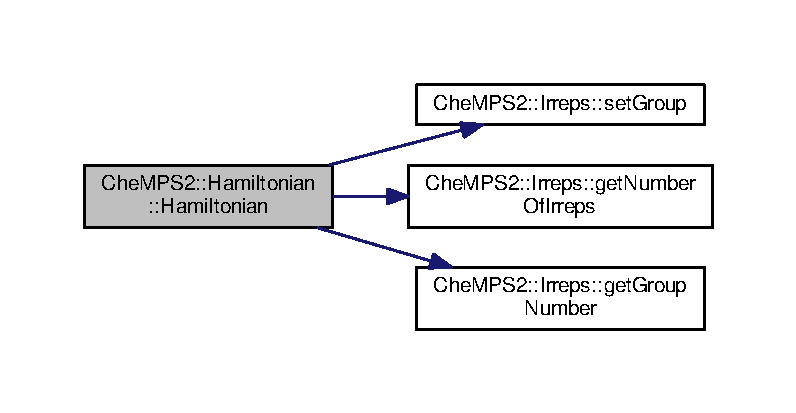
\includegraphics[width=350pt]{classCheMPS2_1_1Hamiltonian_a4ae3520da1ff8515a313c4357592a3d1_cgraph}
\end{center}
\end{figure}


\hypertarget{classCheMPS2_1_1Hamiltonian_a6d20a22b56d996fbd4c9628d4a671a6d}{\index{Che\-M\-P\-S2\-::\-Hamiltonian@{Che\-M\-P\-S2\-::\-Hamiltonian}!Hamiltonian@{Hamiltonian}}
\index{Hamiltonian@{Hamiltonian}!CheMPS2::Hamiltonian@{Che\-M\-P\-S2\-::\-Hamiltonian}}
\paragraph[{Hamiltonian}]{\setlength{\rightskip}{0pt plus 5cm}Che\-M\-P\-S2\-::\-Hamiltonian\-::\-Hamiltonian (
\begin{DoxyParamCaption}
\item[{const string}]{filename}
\end{DoxyParamCaption}
)}}\label{classCheMPS2_1_1Hamiltonian_a6d20a22b56d996fbd4c9628d4a671a6d}


Load an output file created by mointegrals/mointegrals.\-cc; which can be used as a plugin in psi4 beta3. 


\begin{DoxyParams}{Parameters}
{\em filename} & Filename of the psi4 mointegral output file \\
\hline
\end{DoxyParams}


Definition at line 240 of file Hamiltonian.\-cpp.



\subsubsection{Member Function Documentation}
\hypertarget{classCheMPS2_1_1Hamiltonian_ab6147d890404000374bb96baba0b1f82}{\index{Che\-M\-P\-S2\-::\-Hamiltonian@{Che\-M\-P\-S2\-::\-Hamiltonian}!add\-To\-Vmat@{add\-To\-Vmat}}
\index{add\-To\-Vmat@{add\-To\-Vmat}!CheMPS2::Hamiltonian@{Che\-M\-P\-S2\-::\-Hamiltonian}}
\paragraph[{add\-To\-Vmat}]{\setlength{\rightskip}{0pt plus 5cm}void Che\-M\-P\-S2\-::\-Hamiltonian\-::add\-To\-Vmat (
\begin{DoxyParamCaption}
\item[{const int}]{index1, }
\item[{const int}]{index2, }
\item[{const int}]{index3, }
\item[{const int}]{index4, }
\item[{const double}]{val}
\end{DoxyParamCaption}
)}}\label{classCheMPS2_1_1Hamiltonian_ab6147d890404000374bb96baba0b1f82}


Add to Vmat element. 


\begin{DoxyParams}{Parameters}
{\em index1} & The first index \\
\hline
{\em index2} & The second index \\
\hline
{\em index3} & The third index \\
\hline
{\em index4} & The fourth index \\
\hline
{\em val} & The value which should be added \\
\hline
\end{DoxyParams}


Definition at line 117 of file Hamiltonian.\-cpp.

\hypertarget{classCheMPS2_1_1Hamiltonian_a031fa6987b304e3a7f6114b9f2e1f2ab}{\index{Che\-M\-P\-S2\-::\-Hamiltonian@{Che\-M\-P\-S2\-::\-Hamiltonian}!get\-Econst@{get\-Econst}}
\index{get\-Econst@{get\-Econst}!CheMPS2::Hamiltonian@{Che\-M\-P\-S2\-::\-Hamiltonian}}
\paragraph[{get\-Econst}]{\setlength{\rightskip}{0pt plus 5cm}double Che\-M\-P\-S2\-::\-Hamiltonian\-::get\-Econst (
\begin{DoxyParamCaption}
{}
\end{DoxyParamCaption}
) const}}\label{classCheMPS2_1_1Hamiltonian_a031fa6987b304e3a7f6114b9f2e1f2ab}


Get the constant energy. 

\begin{DoxyReturn}{Returns}
The constant part of the \hyperlink{classCheMPS2_1_1Hamiltonian}{Hamiltonian} (nuclear repulsion \& condensed orbitals) 
\end{DoxyReturn}


Definition at line 81 of file Hamiltonian.\-cpp.



Here is the caller graph for this function\-:\nopagebreak
\begin{figure}[H]
\begin{center}
\leavevmode
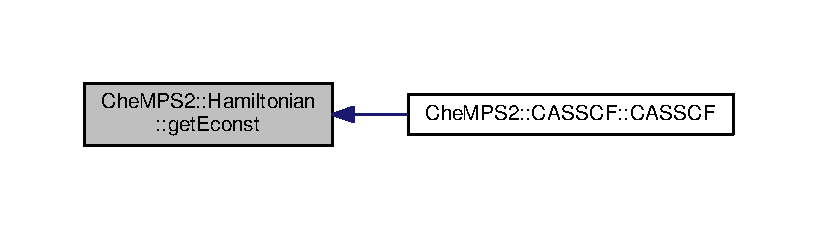
\includegraphics[width=350pt]{classCheMPS2_1_1Hamiltonian_a031fa6987b304e3a7f6114b9f2e1f2ab_icgraph}
\end{center}
\end{figure}


\hypertarget{classCheMPS2_1_1Hamiltonian_a101963cfa8f06abe798a7ae79faab618}{\index{Che\-M\-P\-S2\-::\-Hamiltonian@{Che\-M\-P\-S2\-::\-Hamiltonian}!get\-L@{get\-L}}
\index{get\-L@{get\-L}!CheMPS2::Hamiltonian@{Che\-M\-P\-S2\-::\-Hamiltonian}}
\paragraph[{get\-L}]{\setlength{\rightskip}{0pt plus 5cm}int Che\-M\-P\-S2\-::\-Hamiltonian\-::get\-L (
\begin{DoxyParamCaption}
{}
\end{DoxyParamCaption}
) const}}\label{classCheMPS2_1_1Hamiltonian_a101963cfa8f06abe798a7ae79faab618}


Get the number of orbitals. 

\begin{DoxyReturn}{Returns}
The number of orbitals 
\end{DoxyReturn}


Definition at line 73 of file Hamiltonian.\-cpp.



Here is the caller graph for this function\-:\nopagebreak
\begin{figure}[H]
\begin{center}
\leavevmode
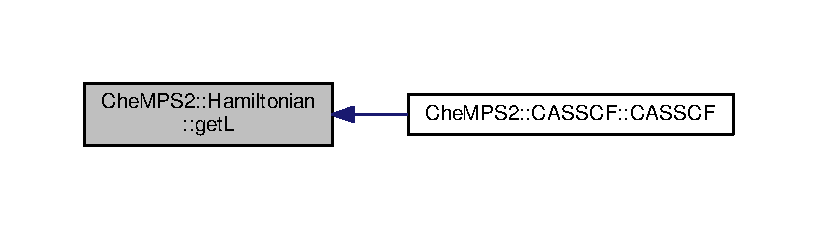
\includegraphics[width=350pt]{classCheMPS2_1_1Hamiltonian_a101963cfa8f06abe798a7ae79faab618_icgraph}
\end{center}
\end{figure}


\hypertarget{classCheMPS2_1_1Hamiltonian_a8c18f51ded63810e316f1834853dce21}{\index{Che\-M\-P\-S2\-::\-Hamiltonian@{Che\-M\-P\-S2\-::\-Hamiltonian}!get\-N\-Group@{get\-N\-Group}}
\index{get\-N\-Group@{get\-N\-Group}!CheMPS2::Hamiltonian@{Che\-M\-P\-S2\-::\-Hamiltonian}}
\paragraph[{get\-N\-Group}]{\setlength{\rightskip}{0pt plus 5cm}int Che\-M\-P\-S2\-::\-Hamiltonian\-::get\-N\-Group (
\begin{DoxyParamCaption}
{}
\end{DoxyParamCaption}
) const}}\label{classCheMPS2_1_1Hamiltonian_a8c18f51ded63810e316f1834853dce21}


Get the group number. 

\begin{DoxyReturn}{Returns}
The group number 
\end{DoxyReturn}


Definition at line 75 of file Hamiltonian.\-cpp.



Here is the caller graph for this function\-:\nopagebreak
\begin{figure}[H]
\begin{center}
\leavevmode
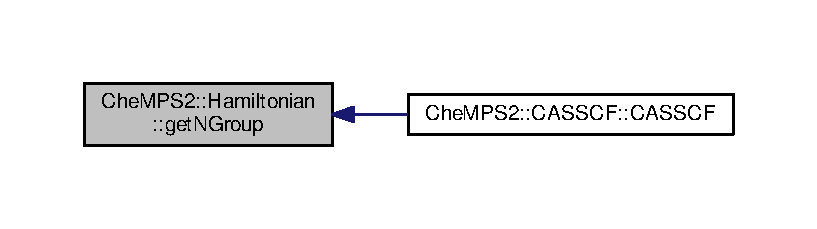
\includegraphics[width=350pt]{classCheMPS2_1_1Hamiltonian_a8c18f51ded63810e316f1834853dce21_icgraph}
\end{center}
\end{figure}


\hypertarget{classCheMPS2_1_1Hamiltonian_a02130b2901a5a3c05171d4f7dd5fa4cd}{\index{Che\-M\-P\-S2\-::\-Hamiltonian@{Che\-M\-P\-S2\-::\-Hamiltonian}!get\-Orbital\-Irrep@{get\-Orbital\-Irrep}}
\index{get\-Orbital\-Irrep@{get\-Orbital\-Irrep}!CheMPS2::Hamiltonian@{Che\-M\-P\-S2\-::\-Hamiltonian}}
\paragraph[{get\-Orbital\-Irrep}]{\setlength{\rightskip}{0pt plus 5cm}int Che\-M\-P\-S2\-::\-Hamiltonian\-::get\-Orbital\-Irrep (
\begin{DoxyParamCaption}
\item[{const int}]{n\-Orb}
\end{DoxyParamCaption}
) const}}\label{classCheMPS2_1_1Hamiltonian_a02130b2901a5a3c05171d4f7dd5fa4cd}


Get an orbital irrep number. 


\begin{DoxyParams}{Parameters}
{\em n\-Orb} & The orbital number \\
\hline
\end{DoxyParams}
\begin{DoxyReturn}{Returns}
The irrep of orbital n\-Orb 
\end{DoxyReturn}


Definition at line 77 of file Hamiltonian.\-cpp.



Here is the caller graph for this function\-:\nopagebreak
\begin{figure}[H]
\begin{center}
\leavevmode
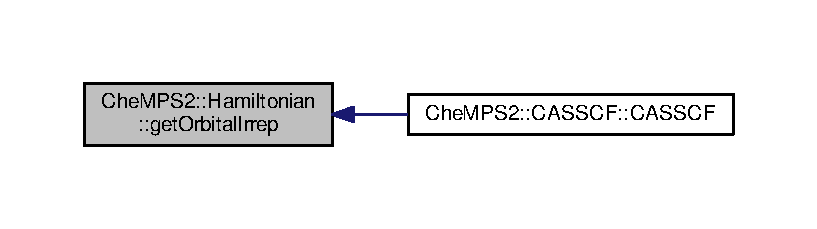
\includegraphics[width=350pt]{classCheMPS2_1_1Hamiltonian_a02130b2901a5a3c05171d4f7dd5fa4cd_icgraph}
\end{center}
\end{figure}


\hypertarget{classCheMPS2_1_1Hamiltonian_ac0b8314dc6133642997e648d1169d10f}{\index{Che\-M\-P\-S2\-::\-Hamiltonian@{Che\-M\-P\-S2\-::\-Hamiltonian}!get\-Tmat@{get\-Tmat}}
\index{get\-Tmat@{get\-Tmat}!CheMPS2::Hamiltonian@{Che\-M\-P\-S2\-::\-Hamiltonian}}
\paragraph[{get\-Tmat}]{\setlength{\rightskip}{0pt plus 5cm}double Che\-M\-P\-S2\-::\-Hamiltonian\-::get\-Tmat (
\begin{DoxyParamCaption}
\item[{const int}]{index1, }
\item[{const int}]{index2}
\end{DoxyParamCaption}
) const}}\label{classCheMPS2_1_1Hamiltonian_ac0b8314dc6133642997e648d1169d10f}


Get a Tmat element. 


\begin{DoxyParams}{Parameters}
{\em index1} & The first index \\
\hline
{\em index2} & The second index \\
\hline
\end{DoxyParams}
\begin{DoxyReturn}{Returns}
$T_{index1,index2}$ 
\end{DoxyReturn}


Definition at line 95 of file Hamiltonian.\-cpp.



Here is the caller graph for this function\-:\nopagebreak
\begin{figure}[H]
\begin{center}
\leavevmode
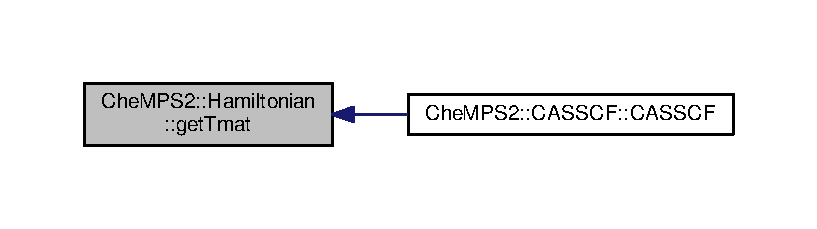
\includegraphics[width=350pt]{classCheMPS2_1_1Hamiltonian_ac0b8314dc6133642997e648d1169d10f_icgraph}
\end{center}
\end{figure}


\hypertarget{classCheMPS2_1_1Hamiltonian_af2d3836be75d50640cbed9a9234af126}{\index{Che\-M\-P\-S2\-::\-Hamiltonian@{Che\-M\-P\-S2\-::\-Hamiltonian}!get\-Vmat@{get\-Vmat}}
\index{get\-Vmat@{get\-Vmat}!CheMPS2::Hamiltonian@{Che\-M\-P\-S2\-::\-Hamiltonian}}
\paragraph[{get\-Vmat}]{\setlength{\rightskip}{0pt plus 5cm}double Che\-M\-P\-S2\-::\-Hamiltonian\-::get\-Vmat (
\begin{DoxyParamCaption}
\item[{const int}]{index1, }
\item[{const int}]{index2, }
\item[{const int}]{index3, }
\item[{const int}]{index4}
\end{DoxyParamCaption}
) const}}\label{classCheMPS2_1_1Hamiltonian_af2d3836be75d50640cbed9a9234af126}


Get a Vmat element. 


\begin{DoxyParams}{Parameters}
{\em index1} & The first index \\
\hline
{\em index2} & The second index \\
\hline
{\em index3} & The third index \\
\hline
{\em index4} & The fourth index \\
\hline
\end{DoxyParams}
\begin{DoxyReturn}{Returns}
$V_{index1,index2,index3,index4}$ 
\end{DoxyReturn}


Definition at line 129 of file Hamiltonian.\-cpp.



Here is the caller graph for this function\-:\nopagebreak
\begin{figure}[H]
\begin{center}
\leavevmode
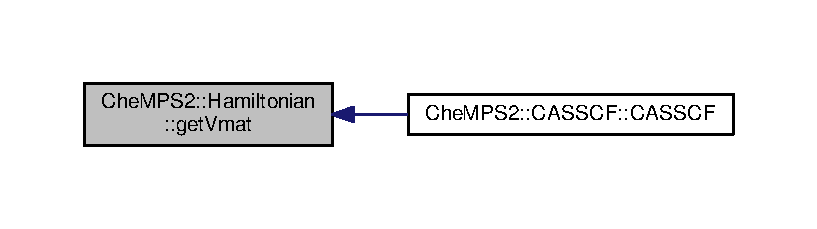
\includegraphics[width=350pt]{classCheMPS2_1_1Hamiltonian_af2d3836be75d50640cbed9a9234af126_icgraph}
\end{center}
\end{figure}


\hypertarget{classCheMPS2_1_1Hamiltonian_af6664242601063dd762c6a430054e4c5}{\index{Che\-M\-P\-S2\-::\-Hamiltonian@{Che\-M\-P\-S2\-::\-Hamiltonian}!set\-Econst@{set\-Econst}}
\index{set\-Econst@{set\-Econst}!CheMPS2::Hamiltonian@{Che\-M\-P\-S2\-::\-Hamiltonian}}
\paragraph[{set\-Econst}]{\setlength{\rightskip}{0pt plus 5cm}void Che\-M\-P\-S2\-::\-Hamiltonian\-::set\-Econst (
\begin{DoxyParamCaption}
\item[{const double}]{val}
\end{DoxyParamCaption}
)}}\label{classCheMPS2_1_1Hamiltonian_af6664242601063dd762c6a430054e4c5}


Set the constant energy. 


\begin{DoxyParams}{Parameters}
{\em val} & The new constant energy \\
\hline
\end{DoxyParams}


Definition at line 79 of file Hamiltonian.\-cpp.

\hypertarget{classCheMPS2_1_1Hamiltonian_a7a56bcf4365125ec144c21d5a4684c32}{\index{Che\-M\-P\-S2\-::\-Hamiltonian@{Che\-M\-P\-S2\-::\-Hamiltonian}!set\-Tmat@{set\-Tmat}}
\index{set\-Tmat@{set\-Tmat}!CheMPS2::Hamiltonian@{Che\-M\-P\-S2\-::\-Hamiltonian}}
\paragraph[{set\-Tmat}]{\setlength{\rightskip}{0pt plus 5cm}void Che\-M\-P\-S2\-::\-Hamiltonian\-::set\-Tmat (
\begin{DoxyParamCaption}
\item[{const int}]{index1, }
\item[{const int}]{index2, }
\item[{const double}]{val}
\end{DoxyParamCaption}
)}}\label{classCheMPS2_1_1Hamiltonian_a7a56bcf4365125ec144c21d5a4684c32}


Set a Tmat element. 


\begin{DoxyParams}{Parameters}
{\em index1} & The first index \\
\hline
{\em index2} & The second index \\
\hline
{\em val} & The new Tmat element \\
\hline
\end{DoxyParams}


Definition at line 83 of file Hamiltonian.\-cpp.

\hypertarget{classCheMPS2_1_1Hamiltonian_a2ddb391c8a20c50bdd2c775cffd8fbb1}{\index{Che\-M\-P\-S2\-::\-Hamiltonian@{Che\-M\-P\-S2\-::\-Hamiltonian}!set\-Vmat@{set\-Vmat}}
\index{set\-Vmat@{set\-Vmat}!CheMPS2::Hamiltonian@{Che\-M\-P\-S2\-::\-Hamiltonian}}
\paragraph[{set\-Vmat}]{\setlength{\rightskip}{0pt plus 5cm}void Che\-M\-P\-S2\-::\-Hamiltonian\-::set\-Vmat (
\begin{DoxyParamCaption}
\item[{const int}]{index1, }
\item[{const int}]{index2, }
\item[{const int}]{index3, }
\item[{const int}]{index4, }
\item[{const double}]{val}
\end{DoxyParamCaption}
)}}\label{classCheMPS2_1_1Hamiltonian_a2ddb391c8a20c50bdd2c775cffd8fbb1}


Set a Vmat element. 


\begin{DoxyParams}{Parameters}
{\em index1} & The first index \\
\hline
{\em index2} & The second index \\
\hline
{\em index3} & The third index \\
\hline
{\em index4} & The fourth index \\
\hline
{\em val} & The new Vmat element \\
\hline
\end{DoxyParams}


Definition at line 105 of file Hamiltonian.\-cpp.



The documentation for this class was generated from the following files\-:\begin{DoxyCompactItemize}
\item 
Hamiltonian.\-h\item 
Hamiltonian.\-cpp\end{DoxyCompactItemize}

\hypertarget{classCheMPS2_1_1Heff}{\subsection{Che\-M\-P\-S2\-:\-:Heff Class Reference}
\label{classCheMPS2_1_1Heff}\index{Che\-M\-P\-S2\-::\-Heff@{Che\-M\-P\-S2\-::\-Heff}}
}


{\ttfamily \#include $<$Heff.\-h$>$}

\subsubsection*{Public Member Functions}
\begin{DoxyCompactItemize}
\item 
\hyperlink{classCheMPS2_1_1Heff_ade178b3ffb362e0b407f50e6393e6f1c}{Heff} (const \hyperlink{classCheMPS2_1_1SyBookkeeper}{Sy\-Bookkeeper} $\ast$den\-B\-K\-In, const \hyperlink{classCheMPS2_1_1Problem}{Problem} $\ast$Prob\-In)
\begin{DoxyCompactList}\small\item\em Constructor. \end{DoxyCompactList}\item 
\hypertarget{classCheMPS2_1_1Heff_aaa1c2a606d65807f669b2a6cbbd9b510}{\hyperlink{classCheMPS2_1_1Heff_aaa1c2a606d65807f669b2a6cbbd9b510}{$\sim$\-Heff} ()}\label{classCheMPS2_1_1Heff_aaa1c2a606d65807f669b2a6cbbd9b510}

\begin{DoxyCompactList}\small\item\em Destructor. \end{DoxyCompactList}\item 
double \hyperlink{classCheMPS2_1_1Heff_ab8ccd23cc035ed40e13705c3f2e581a3}{Solve\-D\-A\-V\-I\-D\-S\-O\-N} (\hyperlink{classCheMPS2_1_1Sobject}{Sobject} $\ast$den\-S, \hyperlink{classCheMPS2_1_1TensorL}{Tensor\-L} $\ast$$\ast$$\ast$Ltensors, \hyperlink{classCheMPS2_1_1TensorA}{Tensor\-A} $\ast$$\ast$$\ast$$\ast$Atensors, \hyperlink{classCheMPS2_1_1TensorB}{Tensor\-B} $\ast$$\ast$$\ast$$\ast$Btensors, \hyperlink{classCheMPS2_1_1TensorC}{Tensor\-C} $\ast$$\ast$$\ast$$\ast$Ctensors, \hyperlink{classCheMPS2_1_1TensorD}{Tensor\-D} $\ast$$\ast$$\ast$$\ast$Dtensors, \hyperlink{classCheMPS2_1_1TensorS0}{Tensor\-S0} $\ast$$\ast$$\ast$$\ast$S0tensors, \hyperlink{classCheMPS2_1_1TensorS1}{Tensor\-S1} $\ast$$\ast$$\ast$$\ast$S1tensors, \hyperlink{classCheMPS2_1_1TensorF0}{Tensor\-F0} $\ast$$\ast$$\ast$$\ast$F0tensors, \hyperlink{classCheMPS2_1_1TensorF1}{Tensor\-F1} $\ast$$\ast$$\ast$$\ast$F1tensors, \hyperlink{classCheMPS2_1_1TensorQ}{Tensor\-Q} $\ast$$\ast$$\ast$Qtensors, \hyperlink{classCheMPS2_1_1TensorX}{Tensor\-X} $\ast$$\ast$Xtensors, int n\-Lower=0, double $\ast$$\ast$Veff\-Tilde=N\-U\-L\-L) const 
\begin{DoxyCompactList}\small\item\em Davidson Solver. \end{DoxyCompactList}\end{DoxyCompactItemize}


\subsubsection{Detailed Description}
\hyperlink{classCheMPS2_1_1Heff}{Heff} class. \begin{DoxyAuthor}{Author}
Sebastian Wouters \href{mailto:sebastianwouters@gmail.com}{\tt sebastianwouters@gmail.\-com} 
\end{DoxyAuthor}
\begin{DoxyDate}{Date}
May 2, 2013
\end{DoxyDate}
The \hyperlink{classCheMPS2_1_1Heff}{Heff} class contains the sparse eigensolver routines and effective \hyperlink{classCheMPS2_1_1Hamiltonian}{Hamiltonian} construction needed for the \hyperlink{classCheMPS2_1_1DMRG}{D\-M\-R\-G} algorithm. 

Definition at line 45 of file Heff.\-h.



\subsubsection{Constructor \& Destructor Documentation}
\hypertarget{classCheMPS2_1_1Heff_ade178b3ffb362e0b407f50e6393e6f1c}{\index{Che\-M\-P\-S2\-::\-Heff@{Che\-M\-P\-S2\-::\-Heff}!Heff@{Heff}}
\index{Heff@{Heff}!CheMPS2::Heff@{Che\-M\-P\-S2\-::\-Heff}}
\paragraph[{Heff}]{\setlength{\rightskip}{0pt plus 5cm}Che\-M\-P\-S2\-::\-Heff\-::\-Heff (
\begin{DoxyParamCaption}
\item[{const {\bf Sy\-Bookkeeper} $\ast$}]{den\-B\-K\-In, }
\item[{const {\bf Problem} $\ast$}]{Prob\-In}
\end{DoxyParamCaption}
)}}\label{classCheMPS2_1_1Heff_ade178b3ffb362e0b407f50e6393e6f1c}


Constructor. 


\begin{DoxyParams}{Parameters}
{\em den\-B\-K\-In} & The \hyperlink{classCheMPS2_1_1SyBookkeeper}{Sy\-Bookkeeper} to get the dimensions \\
\hline
{\em Prob\-In} & The \hyperlink{classCheMPS2_1_1Problem}{Problem} that contains the \hyperlink{classCheMPS2_1_1Hamiltonian}{Hamiltonian} \\
\hline
\end{DoxyParams}


Definition at line 33 of file Heff.\-cpp.



\subsubsection{Member Function Documentation}
\hypertarget{classCheMPS2_1_1Heff_ab8ccd23cc035ed40e13705c3f2e581a3}{\index{Che\-M\-P\-S2\-::\-Heff@{Che\-M\-P\-S2\-::\-Heff}!Solve\-D\-A\-V\-I\-D\-S\-O\-N@{Solve\-D\-A\-V\-I\-D\-S\-O\-N}}
\index{Solve\-D\-A\-V\-I\-D\-S\-O\-N@{Solve\-D\-A\-V\-I\-D\-S\-O\-N}!CheMPS2::Heff@{Che\-M\-P\-S2\-::\-Heff}}
\paragraph[{Solve\-D\-A\-V\-I\-D\-S\-O\-N}]{\setlength{\rightskip}{0pt plus 5cm}double Che\-M\-P\-S2\-::\-Heff\-::\-Solve\-D\-A\-V\-I\-D\-S\-O\-N (
\begin{DoxyParamCaption}
\item[{{\bf Sobject} $\ast$}]{den\-S, }
\item[{{\bf Tensor\-L} $\ast$$\ast$$\ast$}]{Ltensors, }
\item[{{\bf Tensor\-A} $\ast$$\ast$$\ast$$\ast$}]{Atensors, }
\item[{{\bf Tensor\-B} $\ast$$\ast$$\ast$$\ast$}]{Btensors, }
\item[{{\bf Tensor\-C} $\ast$$\ast$$\ast$$\ast$}]{Ctensors, }
\item[{{\bf Tensor\-D} $\ast$$\ast$$\ast$$\ast$}]{Dtensors, }
\item[{{\bf Tensor\-S0} $\ast$$\ast$$\ast$$\ast$}]{S0tensors, }
\item[{{\bf Tensor\-S1} $\ast$$\ast$$\ast$$\ast$}]{S1tensors, }
\item[{{\bf Tensor\-F0} $\ast$$\ast$$\ast$$\ast$}]{F0tensors, }
\item[{{\bf Tensor\-F1} $\ast$$\ast$$\ast$$\ast$}]{F1tensors, }
\item[{{\bf Tensor\-Q} $\ast$$\ast$$\ast$}]{Qtensors, }
\item[{{\bf Tensor\-X} $\ast$$\ast$}]{Xtensors, }
\item[{int}]{n\-Lower = {\ttfamily 0}, }
\item[{double $\ast$$\ast$}]{Veff\-Tilde = {\ttfamily NULL}}
\end{DoxyParamCaption}
) const}}\label{classCheMPS2_1_1Heff_ab8ccd23cc035ed40e13705c3f2e581a3}


Davidson Solver. 


\begin{DoxyParams}{Parameters}
{\em den\-S} & Initial guess S-\/object \\
\hline
{\em Ltensors} & Pointer to the single contracted 2nd quantized operators \\
\hline
{\em Atensors} & Spin-\/0 complementary operators of two creators \\
\hline
{\em Btensors} & Spin-\/1 complementary operators of two creators \\
\hline
{\em Ctensors} & Spin-\/0 complementary operators of a creator and an annihilator \\
\hline
{\em Dtensors} & Spin-\/1 complementary operators of a creator and an annihilator \\
\hline
{\em S0tensors} & Spin-\/0 reduction of two creators \\
\hline
{\em S1tensors} & Spin-\/1 reduction of two creators \\
\hline
{\em F0tensors} & Spin-\/0 reduction of a creator and an annihilator \\
\hline
{\em F1tensors} & Spin-\/1 reduction of a creator and an annihilator \\
\hline
{\em Qtensors} & Complementary operators of three sandwiched 2nd quantized operators \\
\hline
{\em Xtensors} & Pointer to the completely contracted terms \\
\hline
{\em n\-Lower} & Number of lower-\/lying states to project out \\
\hline
{\em Veff\-Tilde} & The projection operators to project the n\-Lower lower-\/lying states out \\
\hline
\end{DoxyParams}


Definition at line 210 of file Heff.\-cpp.



Here is the call graph for this function\-:\nopagebreak
\begin{figure}[H]
\begin{center}
\leavevmode
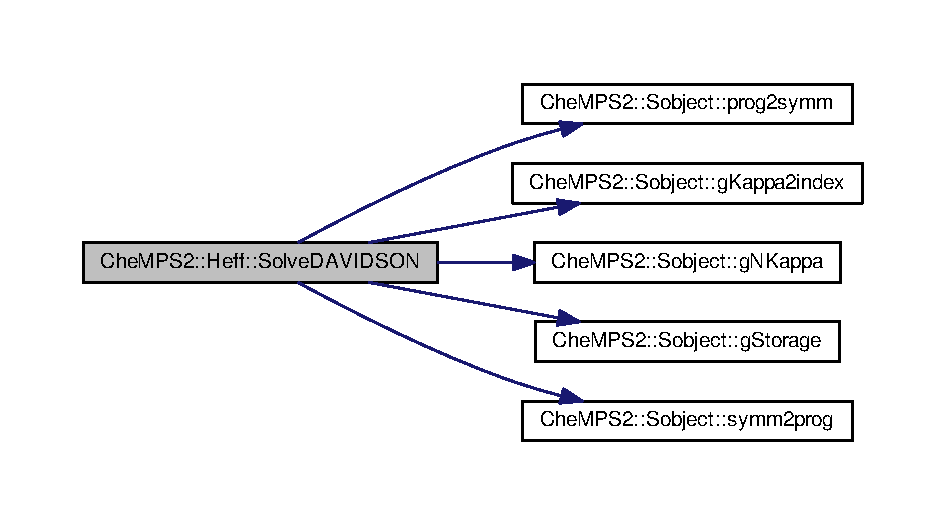
\includegraphics[width=350pt]{classCheMPS2_1_1Heff_ab8ccd23cc035ed40e13705c3f2e581a3_cgraph}
\end{center}
\end{figure}




Here is the caller graph for this function\-:\nopagebreak
\begin{figure}[H]
\begin{center}
\leavevmode
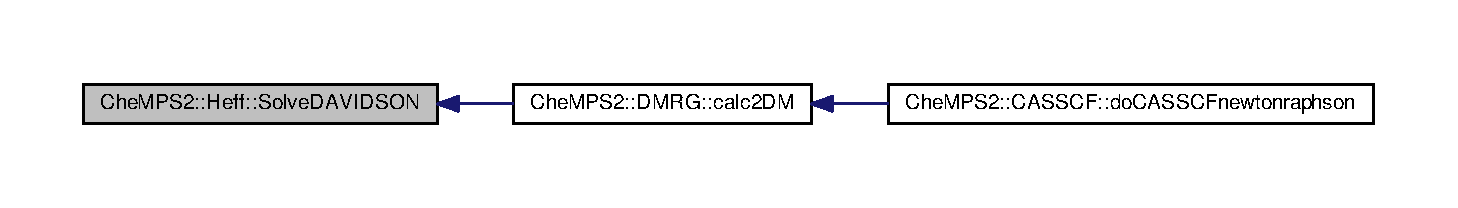
\includegraphics[width=350pt]{classCheMPS2_1_1Heff_ab8ccd23cc035ed40e13705c3f2e581a3_icgraph}
\end{center}
\end{figure}




The documentation for this class was generated from the following files\-:\begin{DoxyCompactItemize}
\item 
Heff.\-h\item 
Heff.\-cpp\item 
Heff\-Diagonal.\-cpp\item 
Heff\-Diagrams1.\-cpp\item 
Heff\-Diagrams2.\-cpp\item 
Heff\-Diagrams3.\-cpp\item 
Heff\-Diagrams4.\-cpp\item 
Heff\-Diagrams5.\-cpp\end{DoxyCompactItemize}

\hypertarget{classCheMPS2_1_1Irreps}{\subsection{Che\-M\-P\-S2\-:\-:Irreps Class Reference}
\label{classCheMPS2_1_1Irreps}\index{Che\-M\-P\-S2\-::\-Irreps@{Che\-M\-P\-S2\-::\-Irreps}}
}


{\ttfamily \#include $<$Irreps.\-h$>$}



Inheritance diagram for Che\-M\-P\-S2\-:\-:Irreps\-:\nopagebreak
\begin{figure}[H]
\begin{center}
\leavevmode
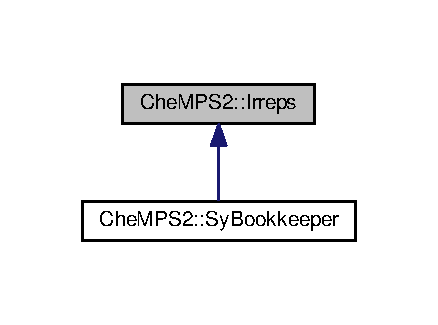
\includegraphics[width=210pt]{classCheMPS2_1_1Irreps__inherit__graph}
\end{center}
\end{figure}
\subsubsection*{Public Member Functions}
\begin{DoxyCompactItemize}
\item 
\hypertarget{classCheMPS2_1_1Irreps_ab84ea352fb5deb5030a9d75809acad40}{\hyperlink{classCheMPS2_1_1Irreps_ab84ea352fb5deb5030a9d75809acad40}{Irreps} ()}\label{classCheMPS2_1_1Irreps_ab84ea352fb5deb5030a9d75809acad40}

\begin{DoxyCompactList}\small\item\em Constructor. \end{DoxyCompactList}\item 
\hyperlink{classCheMPS2_1_1Irreps_a8d33ef5ebd5cf824cf62f3383b455a07}{Irreps} (const int n\-Group)
\begin{DoxyCompactList}\small\item\em Constructor 2. \end{DoxyCompactList}\item 
\hypertarget{classCheMPS2_1_1Irreps_a1bd119362f8477f5d2babe1404ca0826}{virtual \hyperlink{classCheMPS2_1_1Irreps_a1bd119362f8477f5d2babe1404ca0826}{$\sim$\-Irreps} ()}\label{classCheMPS2_1_1Irreps_a1bd119362f8477f5d2babe1404ca0826}

\begin{DoxyCompactList}\small\item\em Destructor. \end{DoxyCompactList}\item 
bool \hyperlink{classCheMPS2_1_1Irreps_aca6fdd79557f9189153258daad5fbe8c}{set\-Group} (const int n\-Group)
\begin{DoxyCompactList}\small\item\em Set the group. \end{DoxyCompactList}\item 
bool \hyperlink{classCheMPS2_1_1Irreps_a4417e98f495d58ac530c73366667e1ae}{get\-Is\-Activated} () const 
\begin{DoxyCompactList}\small\item\em Whether the group number is already activated. \end{DoxyCompactList}\item 
int \hyperlink{classCheMPS2_1_1Irreps_a9813550797b0557cf22d2bca5f3e07b0}{get\-Group\-Number} () const 
\begin{DoxyCompactList}\small\item\em Get the group number. \end{DoxyCompactList}\item 
string \hyperlink{classCheMPS2_1_1Irreps_aa56e8dea52881f0c86c348539b21bb5c}{get\-Group\-Name} () const 
\begin{DoxyCompactList}\small\item\em Get the name of the group. \end{DoxyCompactList}\item 
int \hyperlink{classCheMPS2_1_1Irreps_afd3d1b65e870aad920125c05606c4a7d}{get\-Number\-Of\-Irreps} () const 
\begin{DoxyCompactList}\small\item\em Get the number of irreps for the currently activated group. \end{DoxyCompactList}\item 
string \hyperlink{classCheMPS2_1_1Irreps_acc6050a0690e8e940f9de7cf312bbac4}{get\-Irrep\-Name} (const int irrep\-Number) const 
\begin{DoxyCompactList}\small\item\em Get the name of the irrep with number irrep\-Number of the activated group. The irrep with number 0 is always the trivial irrep. \end{DoxyCompactList}\item 
int \hyperlink{classCheMPS2_1_1Irreps_af639c441270cd0762cb68479ee6a82a6}{direct\-Prod} (const int n1, const int n2) const 
\begin{DoxyCompactList}\small\item\em Get the direct product of the irreps with numbers n1 and n2 for the currently activated group. \end{DoxyCompactList}\end{DoxyCompactItemize}
\subsubsection*{Static Public Member Functions}
\begin{DoxyCompactItemize}
\item 
static string \hyperlink{classCheMPS2_1_1Irreps_a136f15adb9e7f5bcf10af028bb1cec6d}{get\-Group\-Name} (const int n\-Group)
\begin{DoxyCompactList}\small\item\em Get the name of the group corresponding to n\-Group. \end{DoxyCompactList}\item 
static int \hyperlink{classCheMPS2_1_1Irreps_adde5a163d7bc76f80ce73269e9101698}{get\-Trivial\-Irrep} ()
\begin{DoxyCompactList}\small\item\em Get the irrep number of the trivial irrep (always 0) \end{DoxyCompactList}\item 
\hypertarget{classCheMPS2_1_1Irreps_afd70b3b21e33a3f8163db04a768ef848}{static void \hyperlink{classCheMPS2_1_1Irreps_afd70b3b21e33a3f8163db04a768ef848}{print\-All} ()}\label{classCheMPS2_1_1Irreps_afd70b3b21e33a3f8163db04a768ef848}

\begin{DoxyCompactList}\small\item\em Print all info contained in this class. \end{DoxyCompactList}\end{DoxyCompactItemize}


\subsubsection{Detailed Description}
\hyperlink{classCheMPS2_1_1Irreps}{Irreps} class. \begin{DoxyAuthor}{Author}
Sebastian Wouters \href{mailto:sebastianwouters@gmail.com}{\tt sebastianwouters@gmail.\-com} 
\end{DoxyAuthor}
\begin{DoxyDate}{Date}
February 7, 2013
\end{DoxyDate}
Class containing the irrep conventions and multiplication tables. The program requires Abelian point groups with real character tables, with hence $I_{\alpha} \otimes I_{\alpha} = I_{trivial}$.\hypertarget{classCheMPS2_1_1Irreps_irreps_conv}{}\subsubsection{Irrep conventions}\label{classCheMPS2_1_1Irreps_irreps_conv}
The same conventions as in Psi4 (beta3) are used. For convenience, they are listed below\-:\par
 $|$ Group Number \& Name $|$ Irrep Number \& Name $|$ \par
  
\begin{tabular}{|l|cccccccc|}
\hline
         & 0  & 1   & 2   & 3   & 4  & 5   & 6   & 7   \\
\hline
  0: c1  & A  &     &     &     &    &     &     &     \\
  1: ci  & Ag & Au  &     &     &    &     &     &     \\
  2: c2  & A  & B   &     &     &    &     &     &     \\
  3: cs  & A' & A'' &     &     &    &     &     &     \\
  4: d2  & A  & B1  & B2  & B3  &    &     &     &     \\
  5: c2v & A1 & A2  & B1  & B2  &    &     &     &     \\
  6: c2h & Ag & Bg  & Au  & Bu  &    &     &     &     \\
  7: d2h & Ag & B1g & B2g & B3g & Au & B1u & B2u & B3u \\
\hline
\end{tabular}
 

Definition at line 53 of file Irreps.\-h.



\subsubsection{Constructor \& Destructor Documentation}
\hypertarget{classCheMPS2_1_1Irreps_a8d33ef5ebd5cf824cf62f3383b455a07}{\index{Che\-M\-P\-S2\-::\-Irreps@{Che\-M\-P\-S2\-::\-Irreps}!Irreps@{Irreps}}
\index{Irreps@{Irreps}!CheMPS2::Irreps@{Che\-M\-P\-S2\-::\-Irreps}}
\paragraph[{Irreps}]{\setlength{\rightskip}{0pt plus 5cm}Che\-M\-P\-S2\-::\-Irreps\-::\-Irreps (
\begin{DoxyParamCaption}
\item[{const int}]{n\-Group}
\end{DoxyParamCaption}
)}}\label{classCheMPS2_1_1Irreps_a8d33ef5ebd5cf824cf62f3383b455a07}


Constructor 2. 


\begin{DoxyParams}{Parameters}
{\em n\-Group} & The group number (0 $<$= n\-Group $<$= 7; else is\-Activated remains false) \\
\hline
\end{DoxyParams}


Definition at line 36 of file Irreps.\-cpp.



\subsubsection{Member Function Documentation}
\hypertarget{classCheMPS2_1_1Irreps_af639c441270cd0762cb68479ee6a82a6}{\index{Che\-M\-P\-S2\-::\-Irreps@{Che\-M\-P\-S2\-::\-Irreps}!direct\-Prod@{direct\-Prod}}
\index{direct\-Prod@{direct\-Prod}!CheMPS2::Irreps@{Che\-M\-P\-S2\-::\-Irreps}}
\paragraph[{direct\-Prod}]{\setlength{\rightskip}{0pt plus 5cm}int Che\-M\-P\-S2\-::\-Irreps\-::direct\-Prod (
\begin{DoxyParamCaption}
\item[{const int}]{n1, }
\item[{const int}]{n2}
\end{DoxyParamCaption}
) const}}\label{classCheMPS2_1_1Irreps_af639c441270cd0762cb68479ee6a82a6}


Get the direct product of the irreps with numbers n1 and n2 for the currently activated group. 


\begin{DoxyParams}{Parameters}
{\em n1} & The number of the first irrep \\
\hline
{\em n2} & The number of the second irrep \\
\hline
\end{DoxyParams}
\begin{DoxyReturn}{Returns}
The number of the direct product (-\/1 means not activated; -\/2 means n1 or n2 out of bound) 
\end{DoxyReturn}


Definition at line 190 of file Irreps.\-cpp.



Here is the caller graph for this function\-:\nopagebreak
\begin{figure}[H]
\begin{center}
\leavevmode
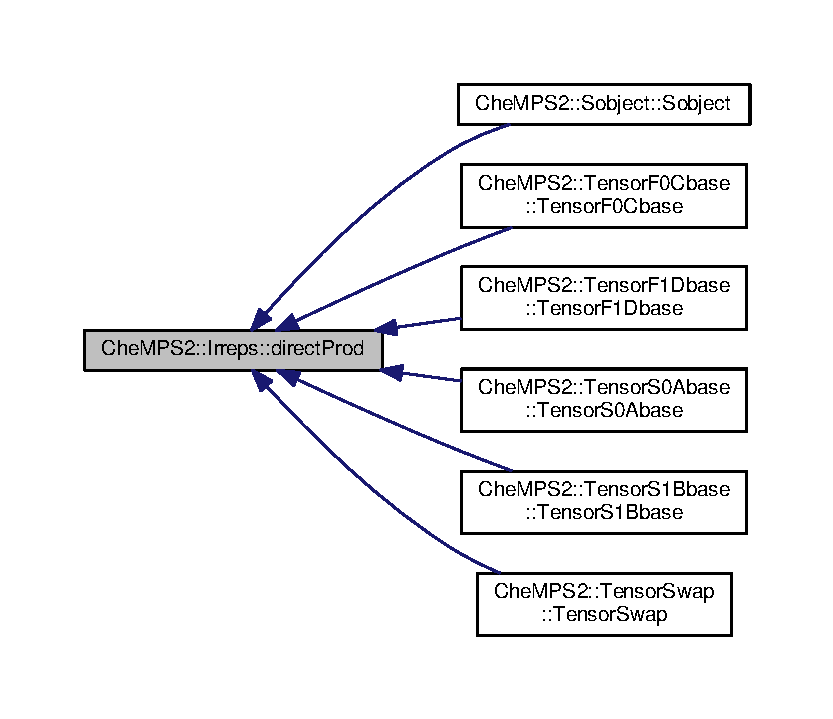
\includegraphics[width=350pt]{classCheMPS2_1_1Irreps_af639c441270cd0762cb68479ee6a82a6_icgraph}
\end{center}
\end{figure}


\hypertarget{classCheMPS2_1_1Irreps_aa56e8dea52881f0c86c348539b21bb5c}{\index{Che\-M\-P\-S2\-::\-Irreps@{Che\-M\-P\-S2\-::\-Irreps}!get\-Group\-Name@{get\-Group\-Name}}
\index{get\-Group\-Name@{get\-Group\-Name}!CheMPS2::Irreps@{Che\-M\-P\-S2\-::\-Irreps}}
\paragraph[{get\-Group\-Name}]{\setlength{\rightskip}{0pt plus 5cm}string Che\-M\-P\-S2\-::\-Irreps\-::get\-Group\-Name (
\begin{DoxyParamCaption}
{}
\end{DoxyParamCaption}
) const}}\label{classCheMPS2_1_1Irreps_aa56e8dea52881f0c86c348539b21bb5c}


Get the name of the group. 

\begin{DoxyReturn}{Returns}
The group name (\char`\"{}error\char`\"{} means not activated) 
\end{DoxyReturn}


Definition at line 76 of file Irreps.\-cpp.

\hypertarget{classCheMPS2_1_1Irreps_a136f15adb9e7f5bcf10af028bb1cec6d}{\index{Che\-M\-P\-S2\-::\-Irreps@{Che\-M\-P\-S2\-::\-Irreps}!get\-Group\-Name@{get\-Group\-Name}}
\index{get\-Group\-Name@{get\-Group\-Name}!CheMPS2::Irreps@{Che\-M\-P\-S2\-::\-Irreps}}
\paragraph[{get\-Group\-Name}]{\setlength{\rightskip}{0pt plus 5cm}string Che\-M\-P\-S2\-::\-Irreps\-::get\-Group\-Name (
\begin{DoxyParamCaption}
\item[{const int}]{n\-Group}
\end{DoxyParamCaption}
)\hspace{0.3cm}{\ttfamily [static]}}}\label{classCheMPS2_1_1Irreps_a136f15adb9e7f5bcf10af028bb1cec6d}


Get the name of the group corresponding to n\-Group. 


\begin{DoxyParams}{Parameters}
{\em n\-Group} & Group number \\
\hline
\end{DoxyParams}
\begin{DoxyReturn}{Returns}
The group name corresponding to n\-Group 
\end{DoxyReturn}


Definition at line 82 of file Irreps.\-cpp.

\hypertarget{classCheMPS2_1_1Irreps_a9813550797b0557cf22d2bca5f3e07b0}{\index{Che\-M\-P\-S2\-::\-Irreps@{Che\-M\-P\-S2\-::\-Irreps}!get\-Group\-Number@{get\-Group\-Number}}
\index{get\-Group\-Number@{get\-Group\-Number}!CheMPS2::Irreps@{Che\-M\-P\-S2\-::\-Irreps}}
\paragraph[{get\-Group\-Number}]{\setlength{\rightskip}{0pt plus 5cm}int Che\-M\-P\-S2\-::\-Irreps\-::get\-Group\-Number (
\begin{DoxyParamCaption}
{}
\end{DoxyParamCaption}
) const}}\label{classCheMPS2_1_1Irreps_a9813550797b0557cf22d2bca5f3e07b0}


Get the group number. 

\begin{DoxyReturn}{Returns}
The group number (-\/1 means not activated) 
\end{DoxyReturn}


Definition at line 70 of file Irreps.\-cpp.



Here is the caller graph for this function\-:\nopagebreak
\begin{figure}[H]
\begin{center}
\leavevmode
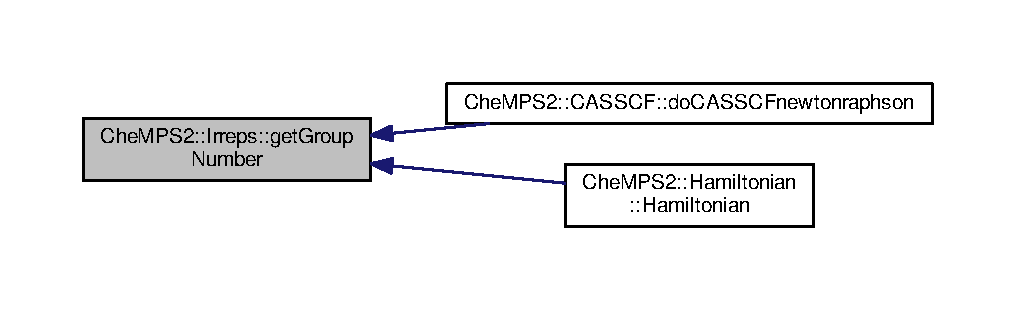
\includegraphics[width=350pt]{classCheMPS2_1_1Irreps_a9813550797b0557cf22d2bca5f3e07b0_icgraph}
\end{center}
\end{figure}


\hypertarget{classCheMPS2_1_1Irreps_acc6050a0690e8e940f9de7cf312bbac4}{\index{Che\-M\-P\-S2\-::\-Irreps@{Che\-M\-P\-S2\-::\-Irreps}!get\-Irrep\-Name@{get\-Irrep\-Name}}
\index{get\-Irrep\-Name@{get\-Irrep\-Name}!CheMPS2::Irreps@{Che\-M\-P\-S2\-::\-Irreps}}
\paragraph[{get\-Irrep\-Name}]{\setlength{\rightskip}{0pt plus 5cm}string Che\-M\-P\-S2\-::\-Irreps\-::get\-Irrep\-Name (
\begin{DoxyParamCaption}
\item[{const int}]{irrep\-Number}
\end{DoxyParamCaption}
) const}}\label{classCheMPS2_1_1Irreps_acc6050a0690e8e940f9de7cf312bbac4}


Get the name of the irrep with number irrep\-Number of the activated group. The irrep with number 0 is always the trivial irrep. 


\begin{DoxyParams}{Parameters}
{\em irrep\-Number} & The irrep number \\
\hline
\end{DoxyParams}
\begin{DoxyReturn}{Returns}
The irrep name (not activated returns \char`\"{}error1\char`\"{}; wrong number returns \char`\"{}error2\char`\"{}) 
\end{DoxyReturn}


Definition at line 117 of file Irreps.\-cpp.

\hypertarget{classCheMPS2_1_1Irreps_a4417e98f495d58ac530c73366667e1ae}{\index{Che\-M\-P\-S2\-::\-Irreps@{Che\-M\-P\-S2\-::\-Irreps}!get\-Is\-Activated@{get\-Is\-Activated}}
\index{get\-Is\-Activated@{get\-Is\-Activated}!CheMPS2::Irreps@{Che\-M\-P\-S2\-::\-Irreps}}
\paragraph[{get\-Is\-Activated}]{\setlength{\rightskip}{0pt plus 5cm}bool Che\-M\-P\-S2\-::\-Irreps\-::get\-Is\-Activated (
\begin{DoxyParamCaption}
{}
\end{DoxyParamCaption}
) const}}\label{classCheMPS2_1_1Irreps_a4417e98f495d58ac530c73366667e1ae}


Whether the group number is already activated. 

\begin{DoxyReturn}{Returns}
Whether the group number is already activated 
\end{DoxyReturn}


Definition at line 64 of file Irreps.\-cpp.

\hypertarget{classCheMPS2_1_1Irreps_afd3d1b65e870aad920125c05606c4a7d}{\index{Che\-M\-P\-S2\-::\-Irreps@{Che\-M\-P\-S2\-::\-Irreps}!get\-Number\-Of\-Irreps@{get\-Number\-Of\-Irreps}}
\index{get\-Number\-Of\-Irreps@{get\-Number\-Of\-Irreps}!CheMPS2::Irreps@{Che\-M\-P\-S2\-::\-Irreps}}
\paragraph[{get\-Number\-Of\-Irreps}]{\setlength{\rightskip}{0pt plus 5cm}int Che\-M\-P\-S2\-::\-Irreps\-::get\-Number\-Of\-Irreps (
\begin{DoxyParamCaption}
{}
\end{DoxyParamCaption}
) const}}\label{classCheMPS2_1_1Irreps_afd3d1b65e870aad920125c05606c4a7d}


Get the number of irreps for the currently activated group. 

\begin{DoxyReturn}{Returns}
The number of irreps for the currently activated group (-\/1 means not activated) 
\end{DoxyReturn}


Definition at line 102 of file Irreps.\-cpp.



Here is the caller graph for this function\-:\nopagebreak
\begin{figure}[H]
\begin{center}
\leavevmode
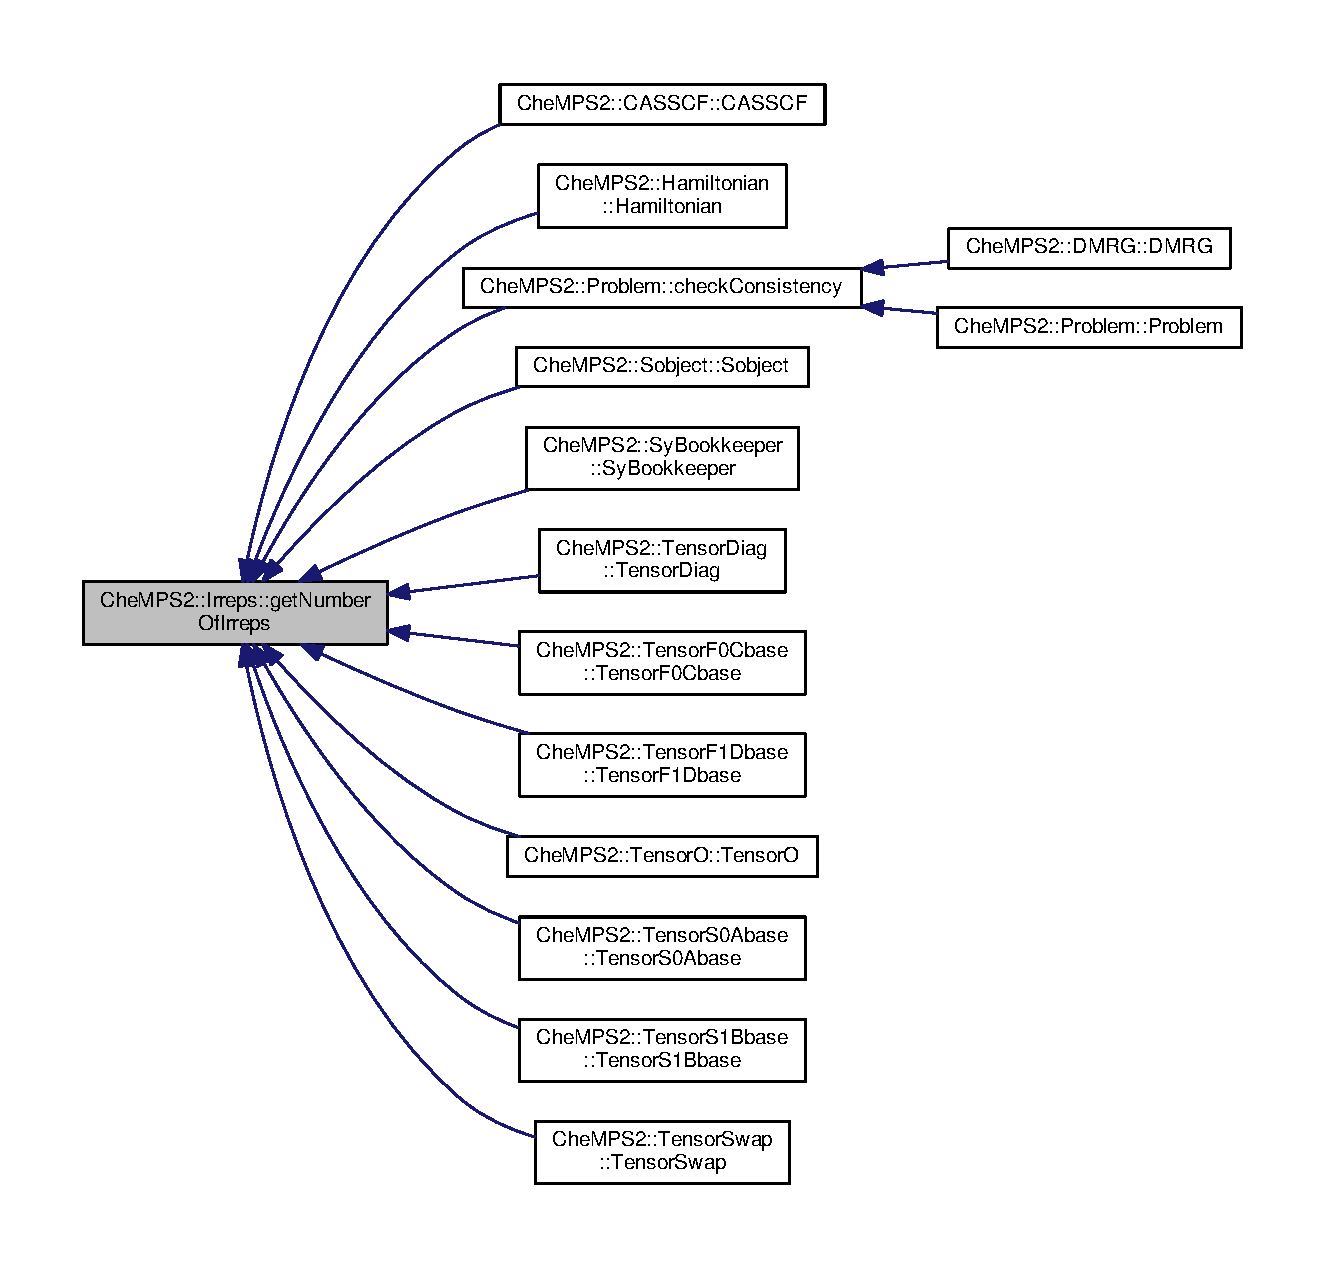
\includegraphics[width=350pt]{classCheMPS2_1_1Irreps_afd3d1b65e870aad920125c05606c4a7d_icgraph}
\end{center}
\end{figure}


\hypertarget{classCheMPS2_1_1Irreps_adde5a163d7bc76f80ce73269e9101698}{\index{Che\-M\-P\-S2\-::\-Irreps@{Che\-M\-P\-S2\-::\-Irreps}!get\-Trivial\-Irrep@{get\-Trivial\-Irrep}}
\index{get\-Trivial\-Irrep@{get\-Trivial\-Irrep}!CheMPS2::Irreps@{Che\-M\-P\-S2\-::\-Irreps}}
\paragraph[{get\-Trivial\-Irrep}]{\setlength{\rightskip}{0pt plus 5cm}int Che\-M\-P\-S2\-::\-Irreps\-::get\-Trivial\-Irrep (
\begin{DoxyParamCaption}
{}
\end{DoxyParamCaption}
)\hspace{0.3cm}{\ttfamily [static]}}}\label{classCheMPS2_1_1Irreps_adde5a163d7bc76f80ce73269e9101698}


Get the irrep number of the trivial irrep (always 0) 

\begin{DoxyReturn}{Returns}
The trivial irrep number 
\end{DoxyReturn}


Definition at line 184 of file Irreps.\-cpp.

\hypertarget{classCheMPS2_1_1Irreps_aca6fdd79557f9189153258daad5fbe8c}{\index{Che\-M\-P\-S2\-::\-Irreps@{Che\-M\-P\-S2\-::\-Irreps}!set\-Group@{set\-Group}}
\index{set\-Group@{set\-Group}!CheMPS2::Irreps@{Che\-M\-P\-S2\-::\-Irreps}}
\paragraph[{set\-Group}]{\setlength{\rightskip}{0pt plus 5cm}bool Che\-M\-P\-S2\-::\-Irreps\-::set\-Group (
\begin{DoxyParamCaption}
\item[{const int}]{n\-Group}
\end{DoxyParamCaption}
)}}\label{classCheMPS2_1_1Irreps_aca6fdd79557f9189153258daad5fbe8c}


Set the group. 


\begin{DoxyParams}{Parameters}
{\em n\-Group} & Number from 0 to 7 (7 included) \\
\hline
\end{DoxyParams}
\begin{DoxyReturn}{Returns}
Validity of the group number (error returns false) 
\end{DoxyReturn}


Definition at line 51 of file Irreps.\-cpp.



Here is the caller graph for this function\-:\nopagebreak
\begin{figure}[H]
\begin{center}
\leavevmode
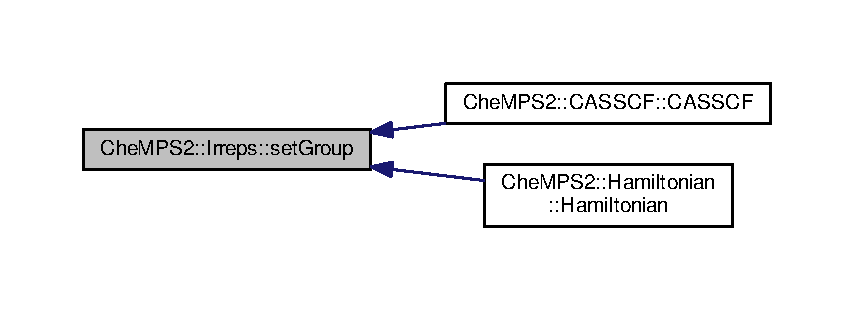
\includegraphics[width=350pt]{classCheMPS2_1_1Irreps_aca6fdd79557f9189153258daad5fbe8c_icgraph}
\end{center}
\end{figure}




The documentation for this class was generated from the following files\-:\begin{DoxyCompactItemize}
\item 
Irreps.\-h\item 
Irreps.\-cpp\end{DoxyCompactItemize}

\hypertarget{classCheMPS2_1_1Problem}{\subsection{Che\-M\-P\-S2\-:\-:Problem Class Reference}
\label{classCheMPS2_1_1Problem}\index{Che\-M\-P\-S2\-::\-Problem@{Che\-M\-P\-S2\-::\-Problem}}
}


{\ttfamily \#include $<$Problem.\-h$>$}

\subsubsection*{Public Member Functions}
\begin{DoxyCompactItemize}
\item 
\hyperlink{classCheMPS2_1_1Problem_aeb177bf0d3fba3520a6fe263a90ee78c}{Problem} (const \hyperlink{classCheMPS2_1_1Hamiltonian}{Hamiltonian} $\ast$Hamin, const int Two\-Sin, const int Nin, const int Irrepin)
\begin{DoxyCompactList}\small\item\em Constructor. \end{DoxyCompactList}\item 
\hypertarget{classCheMPS2_1_1Problem_a9bc13e74cc92e3d697e9cc2ac589afc2}{\hyperlink{classCheMPS2_1_1Problem_a9bc13e74cc92e3d697e9cc2ac589afc2}{$\sim$\-Problem} ()}\label{classCheMPS2_1_1Problem_a9bc13e74cc92e3d697e9cc2ac589afc2}

\begin{DoxyCompactList}\small\item\em Destructor. \end{DoxyCompactList}\item 
int \hyperlink{classCheMPS2_1_1Problem_a3e7be26cd15d22f4e0a65a34616cbcdd}{g\-L} () const 
\begin{DoxyCompactList}\small\item\em Get the number of orbitals. \end{DoxyCompactList}\item 
int \hyperlink{classCheMPS2_1_1Problem_a15485ccb1ac98823b9e8187c16fab03f}{g\-Sy} () const 
\begin{DoxyCompactList}\small\item\em Get the point group symmetry. \end{DoxyCompactList}\item 
int \hyperlink{classCheMPS2_1_1Problem_ac09cc027ab9b41132096e9bd14b549ff}{g\-Irrep} (const int n\-Orb) const 
\begin{DoxyCompactList}\small\item\em Get an orbital irrep. \end{DoxyCompactList}\item 
int \hyperlink{classCheMPS2_1_1Problem_ad472d8f16b1014db3ae67478684b0c49}{g\-Two\-S} () const 
\begin{DoxyCompactList}\small\item\em Get twice the targeted spin. \end{DoxyCompactList}\item 
int \hyperlink{classCheMPS2_1_1Problem_a634bbc2ad8be9f45ecd894f0f222885f}{g\-N} () const 
\begin{DoxyCompactList}\small\item\em Get the targeted particle number. \end{DoxyCompactList}\item 
int \hyperlink{classCheMPS2_1_1Problem_a23de8e37ec94ded22d09328f3d628fad}{g\-Irrep} () const 
\begin{DoxyCompactList}\small\item\em Get the targeted irrep. \end{DoxyCompactList}\item 
double \hyperlink{classCheMPS2_1_1Problem_a6c6f133286114da1666965c8048e47a1}{g\-Econst} () const 
\begin{DoxyCompactList}\small\item\em Get the constant part of the \hyperlink{classCheMPS2_1_1Hamiltonian}{Hamiltonian}. \end{DoxyCompactList}\item 
double \hyperlink{classCheMPS2_1_1Problem_af3ad2a73da9b8af05d145b448cf8bc36}{g\-Mx\-Element} (const int alpha, const int beta, const int gamma, const int delta) const 
\begin{DoxyCompactList}\small\item\em Get a specific interaction matrix element. \end{DoxyCompactList}\item 
bool \hyperlink{classCheMPS2_1_1Problem_a6e26b40eb9bf80eb9979083b58a4e30e}{check\-Consistency} () const 
\begin{DoxyCompactList}\small\item\em Check whether the given parameters L, N, and Two\-S are not inconsistent and whether 0$<$=Irrep$<$n\-Irreps. A more thorough test will be done when the F\-C\-I virtual dimensions are constructed. \end{DoxyCompactList}\item 
bool \hyperlink{classCheMPS2_1_1Problem_ad451eb3fdbd695b938a15515450b6679}{g\-Reorder\-D2h} () const 
\begin{DoxyCompactList}\small\item\em Get whether the \hyperlink{classCheMPS2_1_1Hamiltonian}{Hamiltonian} orbitals are reordered for the \hyperlink{classCheMPS2_1_1DMRG}{D\-M\-R\-G} calculation. \end{DoxyCompactList}\item 
int \hyperlink{classCheMPS2_1_1Problem_af261a2869feffd866b1f7ee5052c9ae9}{gf1} (const int Ham\-Orb) const 
\begin{DoxyCompactList}\small\item\em Get the \hyperlink{classCheMPS2_1_1DMRG}{D\-M\-R\-G} index corresponding to a Ham index. \end{DoxyCompactList}\item 
int \hyperlink{classCheMPS2_1_1Problem_ac5d35cb647b66606e3cf69a21bbcb98a}{gf2} (const int D\-M\-R\-G\-Orb) const 
\begin{DoxyCompactList}\small\item\em Get the Ham index corresponding to a \hyperlink{classCheMPS2_1_1DMRG}{D\-M\-R\-G} index. \end{DoxyCompactList}\item 
\hypertarget{classCheMPS2_1_1Problem_ace8f96e419792f829198e96b897da0a9}{void \hyperlink{classCheMPS2_1_1Problem_ace8f96e419792f829198e96b897da0a9}{Setup\-Reorder\-D2h} ()}\label{classCheMPS2_1_1Problem_ace8f96e419792f829198e96b897da0a9}

\begin{DoxyCompactList}\small\item\em Reorder the orbitals, so that they form irrep blocks, with order of irreps Ag B1u B3u B2g B2u B3g B1g Au. \end{DoxyCompactList}\end{DoxyCompactItemize}


\subsubsection{Detailed Description}
\hyperlink{classCheMPS2_1_1Problem}{Problem} class. \begin{DoxyAuthor}{Author}
Sebastian Wouters \href{mailto:sebastianwouters@gmail.com}{\tt sebastianwouters@gmail.\-com} 
\end{DoxyAuthor}
\begin{DoxyDate}{Date}
February 14, 2013
\end{DoxyDate}
Setup of the problem that is fed to the \hyperlink{classCheMPS2_1_1DMRG}{D\-M\-R\-G} class. It contains
\begin{DoxyItemize}
\item the \hyperlink{classCheMPS2_1_1Hamiltonian}{Hamiltonian}
\item the targeted spin
\item the targeted particle number
\item the targeted wavefunction irrep 
\end{DoxyItemize}

Definition at line 35 of file Problem.\-h.



\subsubsection{Constructor \& Destructor Documentation}
\hypertarget{classCheMPS2_1_1Problem_aeb177bf0d3fba3520a6fe263a90ee78c}{\index{Che\-M\-P\-S2\-::\-Problem@{Che\-M\-P\-S2\-::\-Problem}!Problem@{Problem}}
\index{Problem@{Problem}!CheMPS2::Problem@{Che\-M\-P\-S2\-::\-Problem}}
\paragraph[{Problem}]{\setlength{\rightskip}{0pt plus 5cm}Che\-M\-P\-S2\-::\-Problem\-::\-Problem (
\begin{DoxyParamCaption}
\item[{const {\bf Hamiltonian} $\ast$}]{Hamin, }
\item[{const int}]{Two\-Sin, }
\item[{const int}]{Nin, }
\item[{const int}]{Irrepin}
\end{DoxyParamCaption}
)}}\label{classCheMPS2_1_1Problem_aeb177bf0d3fba3520a6fe263a90ee78c}


Constructor. 


\begin{DoxyParams}{Parameters}
{\em Hamin} & Pointer to the \hyperlink{classCheMPS2_1_1Hamiltonian}{Hamiltonian} \\
\hline
{\em Two\-Sin} & Twice the targeted spin \\
\hline
{\em Nin} & The targeted particle number \\
\hline
{\em Irrepin} & The targeted irrep \\
\hline
\end{DoxyParams}


Definition at line 28 of file Problem.\-cpp.



Here is the call graph for this function\-:\nopagebreak
\begin{figure}[H]
\begin{center}
\leavevmode
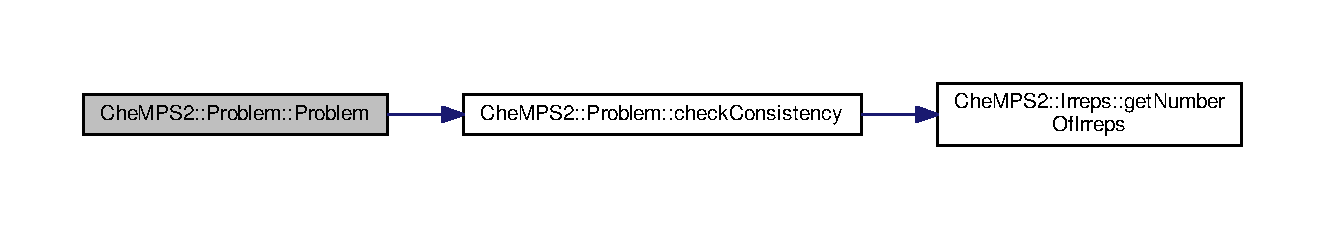
\includegraphics[width=350pt]{classCheMPS2_1_1Problem_aeb177bf0d3fba3520a6fe263a90ee78c_cgraph}
\end{center}
\end{figure}




\subsubsection{Member Function Documentation}
\hypertarget{classCheMPS2_1_1Problem_a6e26b40eb9bf80eb9979083b58a4e30e}{\index{Che\-M\-P\-S2\-::\-Problem@{Che\-M\-P\-S2\-::\-Problem}!check\-Consistency@{check\-Consistency}}
\index{check\-Consistency@{check\-Consistency}!CheMPS2::Problem@{Che\-M\-P\-S2\-::\-Problem}}
\paragraph[{check\-Consistency}]{\setlength{\rightskip}{0pt plus 5cm}bool Che\-M\-P\-S2\-::\-Problem\-::check\-Consistency (
\begin{DoxyParamCaption}
{}
\end{DoxyParamCaption}
) const}}\label{classCheMPS2_1_1Problem_a6e26b40eb9bf80eb9979083b58a4e30e}


Check whether the given parameters L, N, and Two\-S are not inconsistent and whether 0$<$=Irrep$<$n\-Irreps. A more thorough test will be done when the F\-C\-I virtual dimensions are constructed. 

\begin{DoxyReturn}{Returns}
True if consistent, else false 
\end{DoxyReturn}


Definition at line 116 of file Problem.\-cpp.



Here is the call graph for this function\-:\nopagebreak
\begin{figure}[H]
\begin{center}
\leavevmode
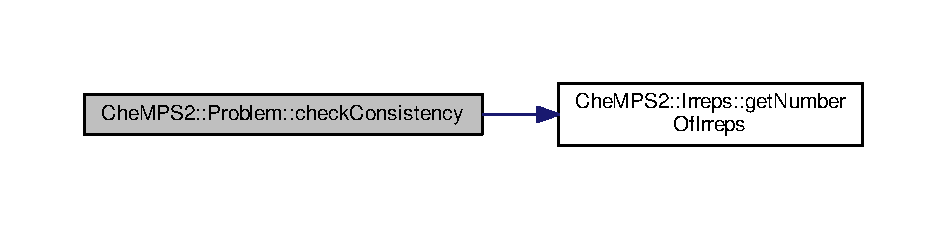
\includegraphics[width=350pt]{classCheMPS2_1_1Problem_a6e26b40eb9bf80eb9979083b58a4e30e_cgraph}
\end{center}
\end{figure}




Here is the caller graph for this function\-:\nopagebreak
\begin{figure}[H]
\begin{center}
\leavevmode
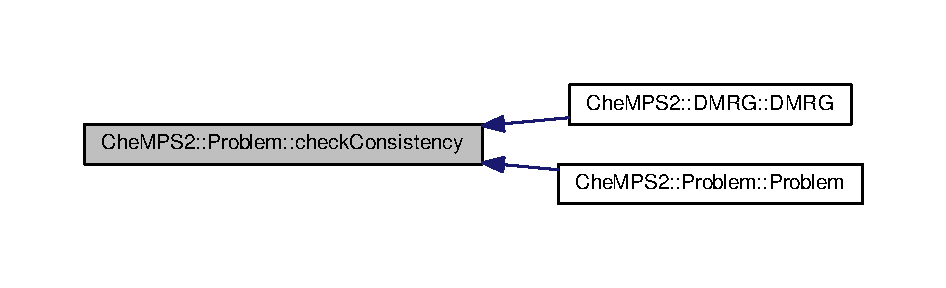
\includegraphics[width=350pt]{classCheMPS2_1_1Problem_a6e26b40eb9bf80eb9979083b58a4e30e_icgraph}
\end{center}
\end{figure}


\hypertarget{classCheMPS2_1_1Problem_a6c6f133286114da1666965c8048e47a1}{\index{Che\-M\-P\-S2\-::\-Problem@{Che\-M\-P\-S2\-::\-Problem}!g\-Econst@{g\-Econst}}
\index{g\-Econst@{g\-Econst}!CheMPS2::Problem@{Che\-M\-P\-S2\-::\-Problem}}
\paragraph[{g\-Econst}]{\setlength{\rightskip}{0pt plus 5cm}double Che\-M\-P\-S2\-::\-Problem\-::g\-Econst (
\begin{DoxyParamCaption}
{}
\end{DoxyParamCaption}
) const}}\label{classCheMPS2_1_1Problem_a6c6f133286114da1666965c8048e47a1}


Get the constant part of the \hyperlink{classCheMPS2_1_1Hamiltonian}{Hamiltonian}. 

\begin{DoxyReturn}{Returns}
The constant part of the \hyperlink{classCheMPS2_1_1Hamiltonian}{Hamiltonian} 
\end{DoxyReturn}


Definition at line 100 of file Problem.\-cpp.



Here is the caller graph for this function\-:\nopagebreak
\begin{figure}[H]
\begin{center}
\leavevmode
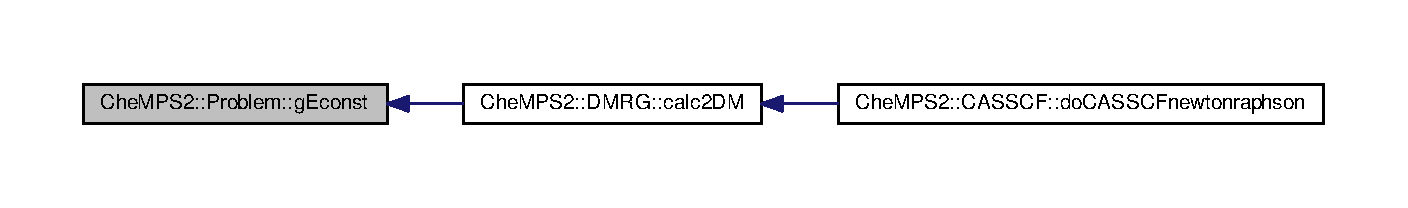
\includegraphics[width=350pt]{classCheMPS2_1_1Problem_a6c6f133286114da1666965c8048e47a1_icgraph}
\end{center}
\end{figure}


\hypertarget{classCheMPS2_1_1Problem_af261a2869feffd866b1f7ee5052c9ae9}{\index{Che\-M\-P\-S2\-::\-Problem@{Che\-M\-P\-S2\-::\-Problem}!gf1@{gf1}}
\index{gf1@{gf1}!CheMPS2::Problem@{Che\-M\-P\-S2\-::\-Problem}}
\paragraph[{gf1}]{\setlength{\rightskip}{0pt plus 5cm}int Che\-M\-P\-S2\-::\-Problem\-::gf1 (
\begin{DoxyParamCaption}
\item[{const int}]{Ham\-Orb}
\end{DoxyParamCaption}
) const}}\label{classCheMPS2_1_1Problem_af261a2869feffd866b1f7ee5052c9ae9}


Get the \hyperlink{classCheMPS2_1_1DMRG}{D\-M\-R\-G} index corresponding to a Ham index. 


\begin{DoxyParams}{Parameters}
{\em Ham\-Orb} & The Ham index \\
\hline
\end{DoxyParams}
\begin{DoxyReturn}{Returns}
The \hyperlink{classCheMPS2_1_1DMRG}{D\-M\-R\-G} index 
\end{DoxyReturn}


Definition at line 103 of file Problem.\-cpp.

\hypertarget{classCheMPS2_1_1Problem_ac5d35cb647b66606e3cf69a21bbcb98a}{\index{Che\-M\-P\-S2\-::\-Problem@{Che\-M\-P\-S2\-::\-Problem}!gf2@{gf2}}
\index{gf2@{gf2}!CheMPS2::Problem@{Che\-M\-P\-S2\-::\-Problem}}
\paragraph[{gf2}]{\setlength{\rightskip}{0pt plus 5cm}int Che\-M\-P\-S2\-::\-Problem\-::gf2 (
\begin{DoxyParamCaption}
\item[{const int}]{D\-M\-R\-G\-Orb}
\end{DoxyParamCaption}
) const}}\label{classCheMPS2_1_1Problem_ac5d35cb647b66606e3cf69a21bbcb98a}


Get the Ham index corresponding to a \hyperlink{classCheMPS2_1_1DMRG}{D\-M\-R\-G} index. 


\begin{DoxyParams}{Parameters}
{\em D\-M\-R\-G\-Orb} & The \hyperlink{classCheMPS2_1_1DMRG}{D\-M\-R\-G} index \\
\hline
\end{DoxyParams}
\begin{DoxyReturn}{Returns}
The Ham index 
\end{DoxyReturn}


Definition at line 104 of file Problem.\-cpp.

\hypertarget{classCheMPS2_1_1Problem_ac09cc027ab9b41132096e9bd14b549ff}{\index{Che\-M\-P\-S2\-::\-Problem@{Che\-M\-P\-S2\-::\-Problem}!g\-Irrep@{g\-Irrep}}
\index{g\-Irrep@{g\-Irrep}!CheMPS2::Problem@{Che\-M\-P\-S2\-::\-Problem}}
\paragraph[{g\-Irrep}]{\setlength{\rightskip}{0pt plus 5cm}int Che\-M\-P\-S2\-::\-Problem\-::g\-Irrep (
\begin{DoxyParamCaption}
\item[{const int}]{n\-Orb}
\end{DoxyParamCaption}
) const}}\label{classCheMPS2_1_1Problem_ac09cc027ab9b41132096e9bd14b549ff}


Get an orbital irrep. 


\begin{DoxyParams}{Parameters}
{\em n\-Orb} & The orbital index \\
\hline
\end{DoxyParams}
\begin{DoxyReturn}{Returns}
The irrep of the orbital with index n\-Orb 
\end{DoxyReturn}


Definition at line 87 of file Problem.\-cpp.

\hypertarget{classCheMPS2_1_1Problem_a23de8e37ec94ded22d09328f3d628fad}{\index{Che\-M\-P\-S2\-::\-Problem@{Che\-M\-P\-S2\-::\-Problem}!g\-Irrep@{g\-Irrep}}
\index{g\-Irrep@{g\-Irrep}!CheMPS2::Problem@{Che\-M\-P\-S2\-::\-Problem}}
\paragraph[{g\-Irrep}]{\setlength{\rightskip}{0pt plus 5cm}int Che\-M\-P\-S2\-::\-Problem\-::g\-Irrep (
\begin{DoxyParamCaption}
{}
\end{DoxyParamCaption}
) const}}\label{classCheMPS2_1_1Problem_a23de8e37ec94ded22d09328f3d628fad}


Get the targeted irrep. 

\begin{DoxyReturn}{Returns}
The targeted irrep 
\end{DoxyReturn}


Definition at line 99 of file Problem.\-cpp.

\hypertarget{classCheMPS2_1_1Problem_a3e7be26cd15d22f4e0a65a34616cbcdd}{\index{Che\-M\-P\-S2\-::\-Problem@{Che\-M\-P\-S2\-::\-Problem}!g\-L@{g\-L}}
\index{g\-L@{g\-L}!CheMPS2::Problem@{Che\-M\-P\-S2\-::\-Problem}}
\paragraph[{g\-L}]{\setlength{\rightskip}{0pt plus 5cm}int Che\-M\-P\-S2\-::\-Problem\-::g\-L (
\begin{DoxyParamCaption}
{}
\end{DoxyParamCaption}
) const}}\label{classCheMPS2_1_1Problem_a3e7be26cd15d22f4e0a65a34616cbcdd}


Get the number of orbitals. 

\begin{DoxyReturn}{Returns}
The number of orbitals 
\end{DoxyReturn}


Definition at line 84 of file Problem.\-cpp.



Here is the caller graph for this function\-:\nopagebreak
\begin{figure}[H]
\begin{center}
\leavevmode
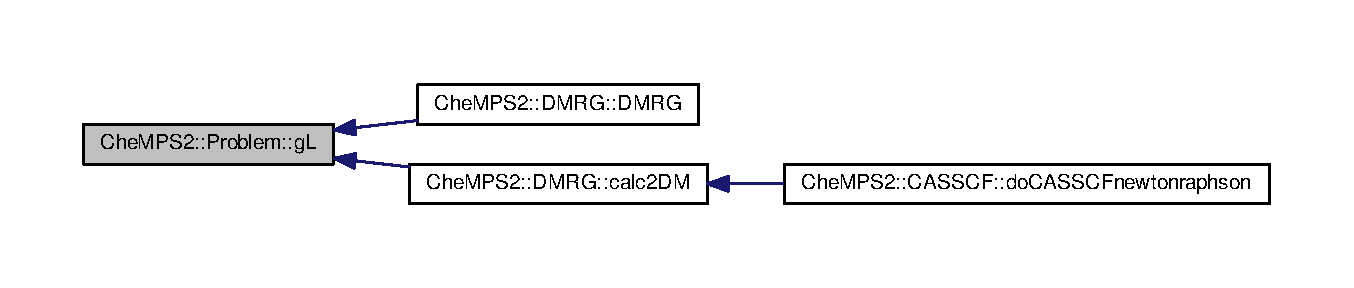
\includegraphics[width=350pt]{classCheMPS2_1_1Problem_a3e7be26cd15d22f4e0a65a34616cbcdd_icgraph}
\end{center}
\end{figure}


\hypertarget{classCheMPS2_1_1Problem_af3ad2a73da9b8af05d145b448cf8bc36}{\index{Che\-M\-P\-S2\-::\-Problem@{Che\-M\-P\-S2\-::\-Problem}!g\-Mx\-Element@{g\-Mx\-Element}}
\index{g\-Mx\-Element@{g\-Mx\-Element}!CheMPS2::Problem@{Che\-M\-P\-S2\-::\-Problem}}
\paragraph[{g\-Mx\-Element}]{\setlength{\rightskip}{0pt plus 5cm}double Che\-M\-P\-S2\-::\-Problem\-::g\-Mx\-Element (
\begin{DoxyParamCaption}
\item[{const int}]{alpha, }
\item[{const int}]{beta, }
\item[{const int}]{gamma, }
\item[{const int}]{delta}
\end{DoxyParamCaption}
) const}}\label{classCheMPS2_1_1Problem_af3ad2a73da9b8af05d145b448cf8bc36}


Get a specific interaction matrix element. 


\begin{DoxyParams}{Parameters}
{\em alpha} & The first index (0 $<$= alpha $<$ L) \\
\hline
{\em beta} & The second index \\
\hline
{\em gamma} & The third index \\
\hline
{\em delta} & The fourth index \\
\hline
\end{DoxyParams}
\begin{DoxyReturn}{Returns}
$ h_{\alpha \beta ; \gamma \delta} = \left(\alpha \beta \mid V \mid \gamma \delta \right) + \frac{1}{N-1} \left( \left( \alpha \mid T \mid \gamma \right) \delta_{\beta \delta} + \delta_{\alpha \gamma} \left( \beta \mid T \mid \delta \right) \right) $ 
\end{DoxyReturn}


Definition at line 106 of file Problem.\-cpp.

\hypertarget{classCheMPS2_1_1Problem_a634bbc2ad8be9f45ecd894f0f222885f}{\index{Che\-M\-P\-S2\-::\-Problem@{Che\-M\-P\-S2\-::\-Problem}!g\-N@{g\-N}}
\index{g\-N@{g\-N}!CheMPS2::Problem@{Che\-M\-P\-S2\-::\-Problem}}
\paragraph[{g\-N}]{\setlength{\rightskip}{0pt plus 5cm}int Che\-M\-P\-S2\-::\-Problem\-::g\-N (
\begin{DoxyParamCaption}
{}
\end{DoxyParamCaption}
) const}}\label{classCheMPS2_1_1Problem_a634bbc2ad8be9f45ecd894f0f222885f}


Get the targeted particle number. 

\begin{DoxyReturn}{Returns}
The targeted particle number 
\end{DoxyReturn}


Definition at line 98 of file Problem.\-cpp.

\hypertarget{classCheMPS2_1_1Problem_ad451eb3fdbd695b938a15515450b6679}{\index{Che\-M\-P\-S2\-::\-Problem@{Che\-M\-P\-S2\-::\-Problem}!g\-Reorder\-D2h@{g\-Reorder\-D2h}}
\index{g\-Reorder\-D2h@{g\-Reorder\-D2h}!CheMPS2::Problem@{Che\-M\-P\-S2\-::\-Problem}}
\paragraph[{g\-Reorder\-D2h}]{\setlength{\rightskip}{0pt plus 5cm}bool Che\-M\-P\-S2\-::\-Problem\-::g\-Reorder\-D2h (
\begin{DoxyParamCaption}
{}
\end{DoxyParamCaption}
) const}}\label{classCheMPS2_1_1Problem_ad451eb3fdbd695b938a15515450b6679}


Get whether the \hyperlink{classCheMPS2_1_1Hamiltonian}{Hamiltonian} orbitals are reordered for the \hyperlink{classCheMPS2_1_1DMRG}{D\-M\-R\-G} calculation. 

\begin{DoxyReturn}{Returns}
Whether the \hyperlink{classCheMPS2_1_1Hamiltonian}{Hamiltonian} orbitals are reordered 
\end{DoxyReturn}


Definition at line 102 of file Problem.\-cpp.

\hypertarget{classCheMPS2_1_1Problem_a15485ccb1ac98823b9e8187c16fab03f}{\index{Che\-M\-P\-S2\-::\-Problem@{Che\-M\-P\-S2\-::\-Problem}!g\-Sy@{g\-Sy}}
\index{g\-Sy@{g\-Sy}!CheMPS2::Problem@{Che\-M\-P\-S2\-::\-Problem}}
\paragraph[{g\-Sy}]{\setlength{\rightskip}{0pt plus 5cm}int Che\-M\-P\-S2\-::\-Problem\-::g\-Sy (
\begin{DoxyParamCaption}
{}
\end{DoxyParamCaption}
) const}}\label{classCheMPS2_1_1Problem_a15485ccb1ac98823b9e8187c16fab03f}


Get the point group symmetry. 

\begin{DoxyReturn}{Returns}
The point group symmetry 
\end{DoxyReturn}


Definition at line 85 of file Problem.\-cpp.

\hypertarget{classCheMPS2_1_1Problem_ad472d8f16b1014db3ae67478684b0c49}{\index{Che\-M\-P\-S2\-::\-Problem@{Che\-M\-P\-S2\-::\-Problem}!g\-Two\-S@{g\-Two\-S}}
\index{g\-Two\-S@{g\-Two\-S}!CheMPS2::Problem@{Che\-M\-P\-S2\-::\-Problem}}
\paragraph[{g\-Two\-S}]{\setlength{\rightskip}{0pt plus 5cm}int Che\-M\-P\-S2\-::\-Problem\-::g\-Two\-S (
\begin{DoxyParamCaption}
{}
\end{DoxyParamCaption}
) const}}\label{classCheMPS2_1_1Problem_ad472d8f16b1014db3ae67478684b0c49}


Get twice the targeted spin. 

\begin{DoxyReturn}{Returns}
Twice the targeted spin 
\end{DoxyReturn}


Definition at line 97 of file Problem.\-cpp.



The documentation for this class was generated from the following files\-:\begin{DoxyCompactItemize}
\item 
Problem.\-h\item 
Problem.\-cpp\end{DoxyCompactItemize}

\hypertarget{classCheMPS2_1_1Sobject}{\subsection{Che\-M\-P\-S2\-:\-:Sobject Class Reference}
\label{classCheMPS2_1_1Sobject}\index{Che\-M\-P\-S2\-::\-Sobject@{Che\-M\-P\-S2\-::\-Sobject}}
}


{\ttfamily \#include $<$Sobject.\-h$>$}

\subsubsection*{Public Member Functions}
\begin{DoxyCompactItemize}
\item 
\hyperlink{classCheMPS2_1_1Sobject_a6fd85753dc9048918065a424c42846d2}{Sobject} (const int index\-In, const int Ilocal\-In1, const int Ilocal\-In2, \hyperlink{classCheMPS2_1_1SyBookkeeper}{Sy\-Bookkeeper} $\ast$den\-B\-K\-In)
\begin{DoxyCompactList}\small\item\em Constructor. \end{DoxyCompactList}\item 
\hypertarget{classCheMPS2_1_1Sobject_a96e39bf1063bb31010cc5c753599f827}{\hyperlink{classCheMPS2_1_1Sobject_a96e39bf1063bb31010cc5c753599f827}{$\sim$\-Sobject} ()}\label{classCheMPS2_1_1Sobject_a96e39bf1063bb31010cc5c753599f827}

\begin{DoxyCompactList}\small\item\em Destructor. \end{DoxyCompactList}\item 
int \hyperlink{classCheMPS2_1_1Sobject_a1dfbe469443fbf7daa49c1d0cb34425e}{g\-N\-Kappa} () const 
\begin{DoxyCompactList}\small\item\em Get the number of symmetry blocks. \end{DoxyCompactList}\item 
double $\ast$ \hyperlink{classCheMPS2_1_1Sobject_a55a31306f564c1d220d36ac9a07623c9}{g\-Storage} ()
\begin{DoxyCompactList}\small\item\em Get the pointer to the storage. \end{DoxyCompactList}\item 
int \hyperlink{classCheMPS2_1_1Sobject_a5626b98bd01a9fb04f4d8e9e739e3034}{g\-Kappa} (const int N\-L, const int Two\-S\-L, const int I\-L, const int N1, const int N2, const int Two\-J, const int N\-R, const int Two\-S\-R, const int I\-R) const 
\begin{DoxyCompactList}\small\item\em Get the index corresponding to a certain symmetry block. \end{DoxyCompactList}\item 
int \hyperlink{classCheMPS2_1_1Sobject_aff81bb404f07da2814b396306fb38588}{g\-Kappa2index} (const int kappa) const 
\begin{DoxyCompactList}\small\item\em Get the storage jump corresponding to a certain symmetry block. \end{DoxyCompactList}\item 
double $\ast$ \hyperlink{classCheMPS2_1_1Sobject_a5a20b20dd98d6ebb67936c525dad5dfc}{g\-Storage} (const int N\-L, const int Two\-S\-L, const int I\-L, const int N1, const int N2, const int Two\-J, const int N\-R, const int Two\-S\-R, const int I\-R)
\begin{DoxyCompactList}\small\item\em Get the pointer to the storage of a certain symmetry block. \end{DoxyCompactList}\item 
int \hyperlink{classCheMPS2_1_1Sobject_a973aa40f2b0e659a55b4c63e768afdf2}{g\-Index} () const 
\begin{DoxyCompactList}\small\item\em Get the location index. \end{DoxyCompactList}\item 
void \hyperlink{classCheMPS2_1_1Sobject_a687a29eab89ef3763af8c630b48e3bf6}{Join} (\hyperlink{classCheMPS2_1_1TensorT}{Tensor\-T} $\ast$Tleft, \hyperlink{classCheMPS2_1_1TensorT}{Tensor\-T} $\ast$Tright)
\begin{DoxyCompactList}\small\item\em Join two sites to form a composite S-\/object. \end{DoxyCompactList}\item 
double \hyperlink{classCheMPS2_1_1Sobject_a34983e86ae9f19de0be6b923479c13df}{Split} (\hyperlink{classCheMPS2_1_1TensorT}{Tensor\-T} $\ast$Tleft, \hyperlink{classCheMPS2_1_1TensorT}{Tensor\-T} $\ast$Tright, const int virtualdimension\-D, const bool movingright, const bool change)
\begin{DoxyCompactList}\small\item\em S\-V\-D an S-\/object into 2 \hyperlink{classCheMPS2_1_1TensorT}{Tensor\-T}'s. \end{DoxyCompactList}\item 
void \hyperlink{classCheMPS2_1_1Sobject_abe676ef06644b5b675c65b123d118f2c}{add\-Noise} (const double Noise\-Level)
\begin{DoxyCompactList}\small\item\em Add noise to the current S-\/object. \end{DoxyCompactList}\item 
\hypertarget{classCheMPS2_1_1Sobject_a01b16408c5439e0eca69b2fde6d0185c}{void \hyperlink{classCheMPS2_1_1Sobject_a01b16408c5439e0eca69b2fde6d0185c}{prog2symm} ()}\label{classCheMPS2_1_1Sobject_a01b16408c5439e0eca69b2fde6d0185c}

\begin{DoxyCompactList}\small\item\em Convert the storage from diagram convention to symmetric \hyperlink{classCheMPS2_1_1Hamiltonian}{Hamiltonian} convention. \end{DoxyCompactList}\item 
\hypertarget{classCheMPS2_1_1Sobject_a2b482f6b45ddd735e42b906843c10e24}{void \hyperlink{classCheMPS2_1_1Sobject_a2b482f6b45ddd735e42b906843c10e24}{symm2prog} ()}\label{classCheMPS2_1_1Sobject_a2b482f6b45ddd735e42b906843c10e24}

\begin{DoxyCompactList}\small\item\em Convert the storage from symmetric \hyperlink{classCheMPS2_1_1Hamiltonian}{Hamiltonian} convention to diagram convention. \end{DoxyCompactList}\item 
int \hyperlink{classCheMPS2_1_1Sobject_a2b8ca2eaecfc448c0f0591462c8edede}{g\-N\-L} (const int ikappa) const 
\begin{DoxyCompactList}\small\item\em Get the left particle number symmetry of block ikappa. \end{DoxyCompactList}\item 
int \hyperlink{classCheMPS2_1_1Sobject_ae33e692d6e5f89d446f62515a85f725f}{g\-Two\-S\-L} (const int ikappa) const 
\begin{DoxyCompactList}\small\item\em Get the left spin symmetry of block ikappa. \end{DoxyCompactList}\item 
int \hyperlink{classCheMPS2_1_1Sobject_a77be4052f1655e2f8fecee8f231bc209}{g\-I\-L} (const int ikappa) const 
\begin{DoxyCompactList}\small\item\em Get the left irrep symmetry of block ikappa. \end{DoxyCompactList}\item 
int \hyperlink{classCheMPS2_1_1Sobject_ae27c30606eb0f3f1eb9a32c559b7b209}{g\-N1} (const int ikappa) const 
\begin{DoxyCompactList}\small\item\em Get the left local particle number symmetry of block ikappa. \end{DoxyCompactList}\item 
int \hyperlink{classCheMPS2_1_1Sobject_a62923e0b950298fe42017dcdeadcfb03}{g\-N2} (const int ikappa) const 
\begin{DoxyCompactList}\small\item\em Get the right local particle number symmetry of block ikappa. \end{DoxyCompactList}\item 
int \hyperlink{classCheMPS2_1_1Sobject_a2bf86bc7861704b1f2ddb655312da82b}{g\-Two\-J} (const int ikappa) const 
\begin{DoxyCompactList}\small\item\em Get the central spin symmetry of block ikappa. \end{DoxyCompactList}\item 
int \hyperlink{classCheMPS2_1_1Sobject_a6dc776c7b9c79a2fb5a5e6e81d190562}{g\-N\-R} (const int ikappa) const 
\begin{DoxyCompactList}\small\item\em Get the right particle number symmetry of block ikappa. \end{DoxyCompactList}\item 
int \hyperlink{classCheMPS2_1_1Sobject_ac3d208dc1bc37fdbcf48aaa9e4cc6ed7}{g\-Two\-S\-R} (const int ikappa) const 
\begin{DoxyCompactList}\small\item\em Get the right spin symmetry of block ikappa. \end{DoxyCompactList}\item 
int \hyperlink{classCheMPS2_1_1Sobject_a1a9a06b257e018439ded8c1bf9c88813}{g\-I\-R} (const int ikappa) const 
\begin{DoxyCompactList}\small\item\em Get the right irrep symmetry of block ikappa. \end{DoxyCompactList}\end{DoxyCompactItemize}


\subsubsection{Detailed Description}
\hyperlink{classCheMPS2_1_1Sobject}{Sobject} class. \begin{DoxyAuthor}{Author}
Sebastian Wouters \href{mailto:sebastianwouters@gmail.com}{\tt sebastianwouters@gmail.\-com} 
\end{DoxyAuthor}
\begin{DoxyDate}{Date}
February 18, 2013
\end{DoxyDate}
Handles the storage of a spin-\/coupled two-\/site object, as is needed for the effective \hyperlink{classCheMPS2_1_1Hamiltonian}{Hamiltonian} \hyperlink{classCheMPS2_1_1DMRG}{D\-M\-R\-G} equations. Extra functionalities are\-:
\begin{DoxyItemize}
\item the formation of an S-\/object out of two neighbouring \hyperlink{classCheMPS2_1_1TensorT}{Tensor\-T}'s
\item the decomposition into two \hyperlink{classCheMPS2_1_1TensorT}{Tensor\-T}'s 
\end{DoxyItemize}

Definition at line 34 of file Sobject.\-h.



\subsubsection{Constructor \& Destructor Documentation}
\hypertarget{classCheMPS2_1_1Sobject_a6fd85753dc9048918065a424c42846d2}{\index{Che\-M\-P\-S2\-::\-Sobject@{Che\-M\-P\-S2\-::\-Sobject}!Sobject@{Sobject}}
\index{Sobject@{Sobject}!CheMPS2::Sobject@{Che\-M\-P\-S2\-::\-Sobject}}
\paragraph[{Sobject}]{\setlength{\rightskip}{0pt plus 5cm}Che\-M\-P\-S2\-::\-Sobject\-::\-Sobject (
\begin{DoxyParamCaption}
\item[{const int}]{index\-In, }
\item[{const int}]{Ilocal\-In1, }
\item[{const int}]{Ilocal\-In2, }
\item[{{\bf Sy\-Bookkeeper} $\ast$}]{den\-B\-K\-In}
\end{DoxyParamCaption}
)}}\label{classCheMPS2_1_1Sobject_a6fd85753dc9048918065a424c42846d2}


Constructor. 


\begin{DoxyParams}{Parameters}
{\em index\-In} & The first index (i ; S spans i \& i+1) \\
\hline
{\em Ilocal\-In1} & The local irrep index of site i \\
\hline
{\em Ilocal\-In2} & The local irrep index of site i+1 \\
\hline
{\em den\-B\-K\-In} & Contains the virtual dimensions. Not const as \hyperlink{classCheMPS2_1_1Sobject}{Sobject} is allowed to set the virtual dimensions of symmetry sectors based on the Schmidt spectrum. \\
\hline
\end{DoxyParams}


Definition at line 33 of file Sobject.\-cpp.



Here is the call graph for this function\-:\nopagebreak
\begin{figure}[H]
\begin{center}
\leavevmode
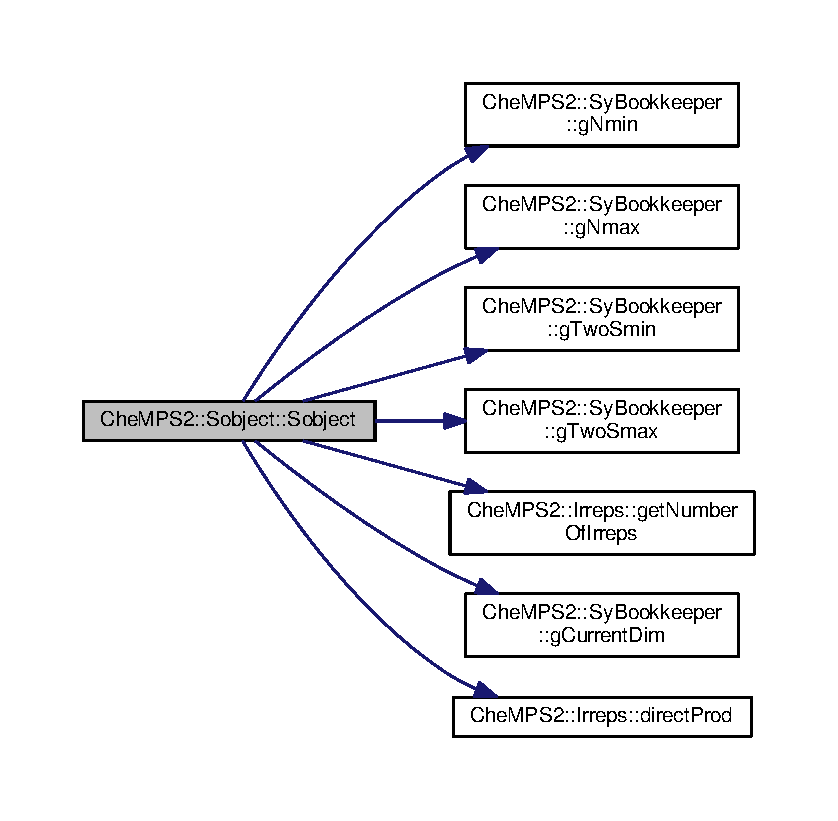
\includegraphics[width=350pt]{classCheMPS2_1_1Sobject_a6fd85753dc9048918065a424c42846d2_cgraph}
\end{center}
\end{figure}




\subsubsection{Member Function Documentation}
\hypertarget{classCheMPS2_1_1Sobject_abe676ef06644b5b675c65b123d118f2c}{\index{Che\-M\-P\-S2\-::\-Sobject@{Che\-M\-P\-S2\-::\-Sobject}!add\-Noise@{add\-Noise}}
\index{add\-Noise@{add\-Noise}!CheMPS2::Sobject@{Che\-M\-P\-S2\-::\-Sobject}}
\paragraph[{add\-Noise}]{\setlength{\rightskip}{0pt plus 5cm}void Che\-M\-P\-S2\-::\-Sobject\-::add\-Noise (
\begin{DoxyParamCaption}
\item[{const double}]{Noise\-Level}
\end{DoxyParamCaption}
)}}\label{classCheMPS2_1_1Sobject_abe676ef06644b5b675c65b123d118f2c}


Add noise to the current S-\/object. 


\begin{DoxyParams}{Parameters}
{\em Noise\-Level} & The noise added to the S-\/object is of size (-\/0.\-5 $<$ random number $<$ 0.\-5) $\ast$ Noise\-Level / infinity-\/norm(\hyperlink{classCheMPS2_1_1Sobject_a55a31306f564c1d220d36ac9a07623c9}{g\-Storage()}) \\
\hline
\end{DoxyParams}


Definition at line 555 of file Sobject.\-cpp.

\hypertarget{classCheMPS2_1_1Sobject_a77be4052f1655e2f8fecee8f231bc209}{\index{Che\-M\-P\-S2\-::\-Sobject@{Che\-M\-P\-S2\-::\-Sobject}!g\-I\-L@{g\-I\-L}}
\index{g\-I\-L@{g\-I\-L}!CheMPS2::Sobject@{Che\-M\-P\-S2\-::\-Sobject}}
\paragraph[{g\-I\-L}]{\setlength{\rightskip}{0pt plus 5cm}int Che\-M\-P\-S2\-::\-Sobject\-::g\-I\-L (
\begin{DoxyParamCaption}
\item[{const int}]{ikappa}
\end{DoxyParamCaption}
) const}}\label{classCheMPS2_1_1Sobject_a77be4052f1655e2f8fecee8f231bc209}


Get the left irrep symmetry of block ikappa. 


\begin{DoxyParams}{Parameters}
{\em ikappa} & The tensor block number \\
\hline
\end{DoxyParams}
\begin{DoxyReturn}{Returns}
the left irrep symmetry of block ikappa 
\end{DoxyReturn}


Definition at line 168 of file Sobject.\-cpp.

\hypertarget{classCheMPS2_1_1Sobject_a973aa40f2b0e659a55b4c63e768afdf2}{\index{Che\-M\-P\-S2\-::\-Sobject@{Che\-M\-P\-S2\-::\-Sobject}!g\-Index@{g\-Index}}
\index{g\-Index@{g\-Index}!CheMPS2::Sobject@{Che\-M\-P\-S2\-::\-Sobject}}
\paragraph[{g\-Index}]{\setlength{\rightskip}{0pt plus 5cm}int Che\-M\-P\-S2\-::\-Sobject\-::g\-Index (
\begin{DoxyParamCaption}
{}
\end{DoxyParamCaption}
) const}}\label{classCheMPS2_1_1Sobject_a973aa40f2b0e659a55b4c63e768afdf2}


Get the location index. 

\begin{DoxyReturn}{Returns}
the index 
\end{DoxyReturn}


Definition at line 164 of file Sobject.\-cpp.

\hypertarget{classCheMPS2_1_1Sobject_a1a9a06b257e018439ded8c1bf9c88813}{\index{Che\-M\-P\-S2\-::\-Sobject@{Che\-M\-P\-S2\-::\-Sobject}!g\-I\-R@{g\-I\-R}}
\index{g\-I\-R@{g\-I\-R}!CheMPS2::Sobject@{Che\-M\-P\-S2\-::\-Sobject}}
\paragraph[{g\-I\-R}]{\setlength{\rightskip}{0pt plus 5cm}int Che\-M\-P\-S2\-::\-Sobject\-::g\-I\-R (
\begin{DoxyParamCaption}
\item[{const int}]{ikappa}
\end{DoxyParamCaption}
) const}}\label{classCheMPS2_1_1Sobject_a1a9a06b257e018439ded8c1bf9c88813}


Get the right irrep symmetry of block ikappa. 


\begin{DoxyParams}{Parameters}
{\em ikappa} & The tensor block number \\
\hline
\end{DoxyParams}
\begin{DoxyReturn}{Returns}
the right irrep symmetry of block ikappa 
\end{DoxyReturn}


Definition at line 174 of file Sobject.\-cpp.

\hypertarget{classCheMPS2_1_1Sobject_a5626b98bd01a9fb04f4d8e9e739e3034}{\index{Che\-M\-P\-S2\-::\-Sobject@{Che\-M\-P\-S2\-::\-Sobject}!g\-Kappa@{g\-Kappa}}
\index{g\-Kappa@{g\-Kappa}!CheMPS2::Sobject@{Che\-M\-P\-S2\-::\-Sobject}}
\paragraph[{g\-Kappa}]{\setlength{\rightskip}{0pt plus 5cm}int Che\-M\-P\-S2\-::\-Sobject\-::g\-Kappa (
\begin{DoxyParamCaption}
\item[{const int}]{N\-L, }
\item[{const int}]{Two\-S\-L, }
\item[{const int}]{I\-L, }
\item[{const int}]{N1, }
\item[{const int}]{N2, }
\item[{const int}]{Two\-J, }
\item[{const int}]{N\-R, }
\item[{const int}]{Two\-S\-R, }
\item[{const int}]{I\-R}
\end{DoxyParamCaption}
) const}}\label{classCheMPS2_1_1Sobject_a5626b98bd01a9fb04f4d8e9e739e3034}


Get the index corresponding to a certain symmetry block. 


\begin{DoxyParams}{Parameters}
{\em N\-L} & The left particle number sector \\
\hline
{\em Two\-S\-L} & The left spin symmetry sector \\
\hline
{\em I\-L} & The left irrep sector \\
\hline
{\em N1} & The first site particle number sector \\
\hline
{\em N2} & The second site particle number sector \\
\hline
{\em Two\-J} & The recoupled two-\/site spin symmetry sector \\
\hline
{\em N\-R} & The right particle number sector \\
\hline
{\em Two\-S\-R} & The right spin symmetry sector \\
\hline
{\em I\-R} & The right irrep sector \\
\hline
\end{DoxyParams}
\begin{DoxyReturn}{Returns}
The kappa corresponding to the input parameters; -\/1 means no such block 
\end{DoxyReturn}


Definition at line 144 of file Sobject.\-cpp.

\hypertarget{classCheMPS2_1_1Sobject_aff81bb404f07da2814b396306fb38588}{\index{Che\-M\-P\-S2\-::\-Sobject@{Che\-M\-P\-S2\-::\-Sobject}!g\-Kappa2index@{g\-Kappa2index}}
\index{g\-Kappa2index@{g\-Kappa2index}!CheMPS2::Sobject@{Che\-M\-P\-S2\-::\-Sobject}}
\paragraph[{g\-Kappa2index}]{\setlength{\rightskip}{0pt plus 5cm}int Che\-M\-P\-S2\-::\-Sobject\-::g\-Kappa2index (
\begin{DoxyParamCaption}
\item[{const int}]{kappa}
\end{DoxyParamCaption}
) const}}\label{classCheMPS2_1_1Sobject_aff81bb404f07da2814b396306fb38588}


Get the storage jump corresponding to a certain symmetry block. 


\begin{DoxyParams}{Parameters}
{\em kappa} & The symmetry block \\
\hline
\end{DoxyParams}
\begin{DoxyReturn}{Returns}
kappa2index\mbox{[}kappa\mbox{]}, the memory jumper to a certain block 
\end{DoxyReturn}


Definition at line 154 of file Sobject.\-cpp.



Here is the caller graph for this function\-:\nopagebreak
\begin{figure}[H]
\begin{center}
\leavevmode
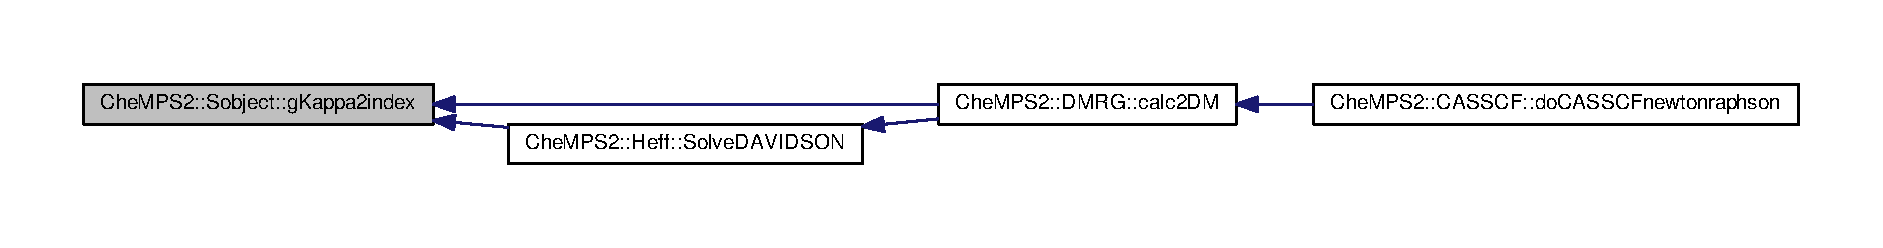
\includegraphics[width=350pt]{classCheMPS2_1_1Sobject_aff81bb404f07da2814b396306fb38588_icgraph}
\end{center}
\end{figure}


\hypertarget{classCheMPS2_1_1Sobject_ae27c30606eb0f3f1eb9a32c559b7b209}{\index{Che\-M\-P\-S2\-::\-Sobject@{Che\-M\-P\-S2\-::\-Sobject}!g\-N1@{g\-N1}}
\index{g\-N1@{g\-N1}!CheMPS2::Sobject@{Che\-M\-P\-S2\-::\-Sobject}}
\paragraph[{g\-N1}]{\setlength{\rightskip}{0pt plus 5cm}int Che\-M\-P\-S2\-::\-Sobject\-::g\-N1 (
\begin{DoxyParamCaption}
\item[{const int}]{ikappa}
\end{DoxyParamCaption}
) const}}\label{classCheMPS2_1_1Sobject_ae27c30606eb0f3f1eb9a32c559b7b209}


Get the left local particle number symmetry of block ikappa. 


\begin{DoxyParams}{Parameters}
{\em ikappa} & The tensor block number \\
\hline
\end{DoxyParams}
\begin{DoxyReturn}{Returns}
the left local particle number symmetry of block ikappa 
\end{DoxyReturn}


Definition at line 169 of file Sobject.\-cpp.

\hypertarget{classCheMPS2_1_1Sobject_a62923e0b950298fe42017dcdeadcfb03}{\index{Che\-M\-P\-S2\-::\-Sobject@{Che\-M\-P\-S2\-::\-Sobject}!g\-N2@{g\-N2}}
\index{g\-N2@{g\-N2}!CheMPS2::Sobject@{Che\-M\-P\-S2\-::\-Sobject}}
\paragraph[{g\-N2}]{\setlength{\rightskip}{0pt plus 5cm}int Che\-M\-P\-S2\-::\-Sobject\-::g\-N2 (
\begin{DoxyParamCaption}
\item[{const int}]{ikappa}
\end{DoxyParamCaption}
) const}}\label{classCheMPS2_1_1Sobject_a62923e0b950298fe42017dcdeadcfb03}


Get the right local particle number symmetry of block ikappa. 


\begin{DoxyParams}{Parameters}
{\em ikappa} & The tensor block number \\
\hline
\end{DoxyParams}
\begin{DoxyReturn}{Returns}
the right local particle number symmetry of block ikappa 
\end{DoxyReturn}


Definition at line 170 of file Sobject.\-cpp.

\hypertarget{classCheMPS2_1_1Sobject_a1dfbe469443fbf7daa49c1d0cb34425e}{\index{Che\-M\-P\-S2\-::\-Sobject@{Che\-M\-P\-S2\-::\-Sobject}!g\-N\-Kappa@{g\-N\-Kappa}}
\index{g\-N\-Kappa@{g\-N\-Kappa}!CheMPS2::Sobject@{Che\-M\-P\-S2\-::\-Sobject}}
\paragraph[{g\-N\-Kappa}]{\setlength{\rightskip}{0pt plus 5cm}int Che\-M\-P\-S2\-::\-Sobject\-::g\-N\-Kappa (
\begin{DoxyParamCaption}
{}
\end{DoxyParamCaption}
) const}}\label{classCheMPS2_1_1Sobject_a1dfbe469443fbf7daa49c1d0cb34425e}


Get the number of symmetry blocks. 

\begin{DoxyReturn}{Returns}
The number of symmetry blocks 
\end{DoxyReturn}


Definition at line 140 of file Sobject.\-cpp.



Here is the caller graph for this function\-:\nopagebreak
\begin{figure}[H]
\begin{center}
\leavevmode
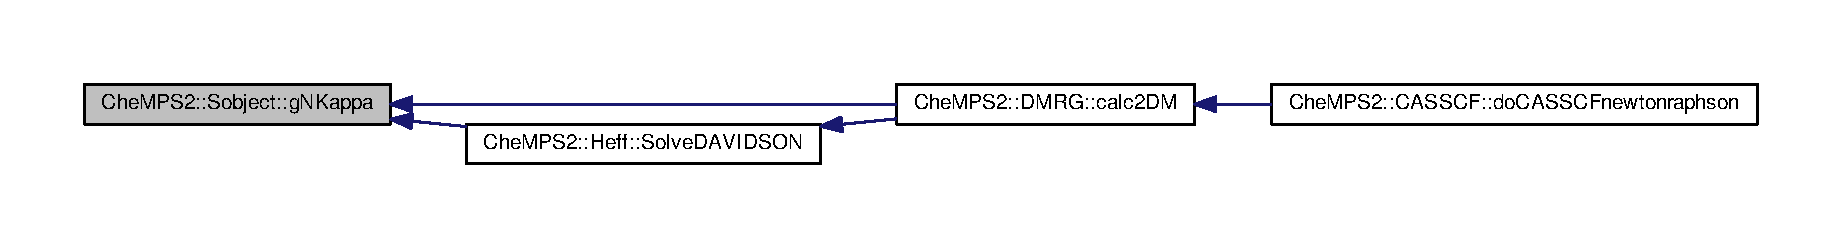
\includegraphics[width=350pt]{classCheMPS2_1_1Sobject_a1dfbe469443fbf7daa49c1d0cb34425e_icgraph}
\end{center}
\end{figure}


\hypertarget{classCheMPS2_1_1Sobject_a2b8ca2eaecfc448c0f0591462c8edede}{\index{Che\-M\-P\-S2\-::\-Sobject@{Che\-M\-P\-S2\-::\-Sobject}!g\-N\-L@{g\-N\-L}}
\index{g\-N\-L@{g\-N\-L}!CheMPS2::Sobject@{Che\-M\-P\-S2\-::\-Sobject}}
\paragraph[{g\-N\-L}]{\setlength{\rightskip}{0pt plus 5cm}int Che\-M\-P\-S2\-::\-Sobject\-::g\-N\-L (
\begin{DoxyParamCaption}
\item[{const int}]{ikappa}
\end{DoxyParamCaption}
) const}}\label{classCheMPS2_1_1Sobject_a2b8ca2eaecfc448c0f0591462c8edede}


Get the left particle number symmetry of block ikappa. 


\begin{DoxyParams}{Parameters}
{\em ikappa} & The tensor block number \\
\hline
\end{DoxyParams}
\begin{DoxyReturn}{Returns}
the left particle number symmetry of block ikappa 
\end{DoxyReturn}


Definition at line 166 of file Sobject.\-cpp.

\hypertarget{classCheMPS2_1_1Sobject_a6dc776c7b9c79a2fb5a5e6e81d190562}{\index{Che\-M\-P\-S2\-::\-Sobject@{Che\-M\-P\-S2\-::\-Sobject}!g\-N\-R@{g\-N\-R}}
\index{g\-N\-R@{g\-N\-R}!CheMPS2::Sobject@{Che\-M\-P\-S2\-::\-Sobject}}
\paragraph[{g\-N\-R}]{\setlength{\rightskip}{0pt plus 5cm}int Che\-M\-P\-S2\-::\-Sobject\-::g\-N\-R (
\begin{DoxyParamCaption}
\item[{const int}]{ikappa}
\end{DoxyParamCaption}
) const}}\label{classCheMPS2_1_1Sobject_a6dc776c7b9c79a2fb5a5e6e81d190562}


Get the right particle number symmetry of block ikappa. 


\begin{DoxyParams}{Parameters}
{\em ikappa} & The tensor block number \\
\hline
\end{DoxyParams}
\begin{DoxyReturn}{Returns}
the right particle number symmetry of block ikappa 
\end{DoxyReturn}


Definition at line 172 of file Sobject.\-cpp.

\hypertarget{classCheMPS2_1_1Sobject_a55a31306f564c1d220d36ac9a07623c9}{\index{Che\-M\-P\-S2\-::\-Sobject@{Che\-M\-P\-S2\-::\-Sobject}!g\-Storage@{g\-Storage}}
\index{g\-Storage@{g\-Storage}!CheMPS2::Sobject@{Che\-M\-P\-S2\-::\-Sobject}}
\paragraph[{g\-Storage}]{\setlength{\rightskip}{0pt plus 5cm}double $\ast$ Che\-M\-P\-S2\-::\-Sobject\-::g\-Storage (
\begin{DoxyParamCaption}
{}
\end{DoxyParamCaption}
)}}\label{classCheMPS2_1_1Sobject_a55a31306f564c1d220d36ac9a07623c9}


Get the pointer to the storage. 

return pointer to the storage 

Definition at line 142 of file Sobject.\-cpp.



Here is the caller graph for this function\-:\nopagebreak
\begin{figure}[H]
\begin{center}
\leavevmode
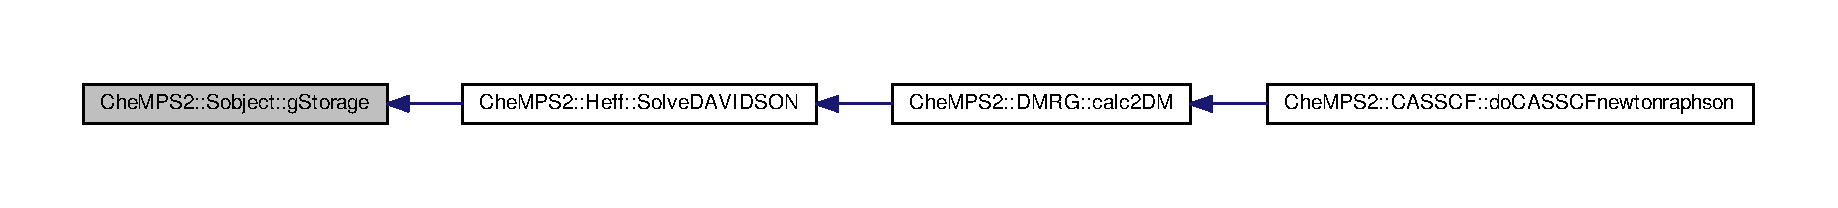
\includegraphics[width=350pt]{classCheMPS2_1_1Sobject_a55a31306f564c1d220d36ac9a07623c9_icgraph}
\end{center}
\end{figure}


\hypertarget{classCheMPS2_1_1Sobject_a5a20b20dd98d6ebb67936c525dad5dfc}{\index{Che\-M\-P\-S2\-::\-Sobject@{Che\-M\-P\-S2\-::\-Sobject}!g\-Storage@{g\-Storage}}
\index{g\-Storage@{g\-Storage}!CheMPS2::Sobject@{Che\-M\-P\-S2\-::\-Sobject}}
\paragraph[{g\-Storage}]{\setlength{\rightskip}{0pt plus 5cm}double $\ast$ Che\-M\-P\-S2\-::\-Sobject\-::g\-Storage (
\begin{DoxyParamCaption}
\item[{const int}]{N\-L, }
\item[{const int}]{Two\-S\-L, }
\item[{const int}]{I\-L, }
\item[{const int}]{N1, }
\item[{const int}]{N2, }
\item[{const int}]{Two\-J, }
\item[{const int}]{N\-R, }
\item[{const int}]{Two\-S\-R, }
\item[{const int}]{I\-R}
\end{DoxyParamCaption}
)}}\label{classCheMPS2_1_1Sobject_a5a20b20dd98d6ebb67936c525dad5dfc}


Get the pointer to the storage of a certain symmetry block. 


\begin{DoxyParams}{Parameters}
{\em N\-L} & The left particle number sector \\
\hline
{\em Two\-S\-L} & The left spin symmetry sector \\
\hline
{\em I\-L} & The left irrep sector \\
\hline
{\em N1} & The first site particle number sector \\
\hline
{\em N2} & The second site particle number sector \\
\hline
{\em Two\-J} & The recoupled two-\/site spin symmetry sector \\
\hline
{\em N\-R} & The right particle number sector \\
\hline
{\em Two\-S\-R} & The right spin symmetry sector \\
\hline
{\em I\-R} & The right irrep sector \\
\hline
\end{DoxyParams}
\begin{DoxyReturn}{Returns}
Pointer to the requested block; N\-U\-L\-L means no such block (kappa == -\/1) 
\end{DoxyReturn}


Definition at line 156 of file Sobject.\-cpp.

\hypertarget{classCheMPS2_1_1Sobject_a2bf86bc7861704b1f2ddb655312da82b}{\index{Che\-M\-P\-S2\-::\-Sobject@{Che\-M\-P\-S2\-::\-Sobject}!g\-Two\-J@{g\-Two\-J}}
\index{g\-Two\-J@{g\-Two\-J}!CheMPS2::Sobject@{Che\-M\-P\-S2\-::\-Sobject}}
\paragraph[{g\-Two\-J}]{\setlength{\rightskip}{0pt plus 5cm}int Che\-M\-P\-S2\-::\-Sobject\-::g\-Two\-J (
\begin{DoxyParamCaption}
\item[{const int}]{ikappa}
\end{DoxyParamCaption}
) const}}\label{classCheMPS2_1_1Sobject_a2bf86bc7861704b1f2ddb655312da82b}


Get the central spin symmetry of block ikappa. 


\begin{DoxyParams}{Parameters}
{\em ikappa} & The tensor block number \\
\hline
\end{DoxyParams}
\begin{DoxyReturn}{Returns}
the central spin symmetry of block ikappa 
\end{DoxyReturn}


Definition at line 171 of file Sobject.\-cpp.

\hypertarget{classCheMPS2_1_1Sobject_ae33e692d6e5f89d446f62515a85f725f}{\index{Che\-M\-P\-S2\-::\-Sobject@{Che\-M\-P\-S2\-::\-Sobject}!g\-Two\-S\-L@{g\-Two\-S\-L}}
\index{g\-Two\-S\-L@{g\-Two\-S\-L}!CheMPS2::Sobject@{Che\-M\-P\-S2\-::\-Sobject}}
\paragraph[{g\-Two\-S\-L}]{\setlength{\rightskip}{0pt plus 5cm}int Che\-M\-P\-S2\-::\-Sobject\-::g\-Two\-S\-L (
\begin{DoxyParamCaption}
\item[{const int}]{ikappa}
\end{DoxyParamCaption}
) const}}\label{classCheMPS2_1_1Sobject_ae33e692d6e5f89d446f62515a85f725f}


Get the left spin symmetry of block ikappa. 


\begin{DoxyParams}{Parameters}
{\em ikappa} & The tensor block number \\
\hline
\end{DoxyParams}
\begin{DoxyReturn}{Returns}
the left spin symmetry of block ikappa 
\end{DoxyReturn}


Definition at line 167 of file Sobject.\-cpp.

\hypertarget{classCheMPS2_1_1Sobject_ac3d208dc1bc37fdbcf48aaa9e4cc6ed7}{\index{Che\-M\-P\-S2\-::\-Sobject@{Che\-M\-P\-S2\-::\-Sobject}!g\-Two\-S\-R@{g\-Two\-S\-R}}
\index{g\-Two\-S\-R@{g\-Two\-S\-R}!CheMPS2::Sobject@{Che\-M\-P\-S2\-::\-Sobject}}
\paragraph[{g\-Two\-S\-R}]{\setlength{\rightskip}{0pt plus 5cm}int Che\-M\-P\-S2\-::\-Sobject\-::g\-Two\-S\-R (
\begin{DoxyParamCaption}
\item[{const int}]{ikappa}
\end{DoxyParamCaption}
) const}}\label{classCheMPS2_1_1Sobject_ac3d208dc1bc37fdbcf48aaa9e4cc6ed7}


Get the right spin symmetry of block ikappa. 


\begin{DoxyParams}{Parameters}
{\em ikappa} & The tensor block number \\
\hline
\end{DoxyParams}
\begin{DoxyReturn}{Returns}
the right spin symmetry of block ikappa 
\end{DoxyReturn}


Definition at line 173 of file Sobject.\-cpp.

\hypertarget{classCheMPS2_1_1Sobject_a687a29eab89ef3763af8c630b48e3bf6}{\index{Che\-M\-P\-S2\-::\-Sobject@{Che\-M\-P\-S2\-::\-Sobject}!Join@{Join}}
\index{Join@{Join}!CheMPS2::Sobject@{Che\-M\-P\-S2\-::\-Sobject}}
\paragraph[{Join}]{\setlength{\rightskip}{0pt plus 5cm}void Che\-M\-P\-S2\-::\-Sobject\-::\-Join (
\begin{DoxyParamCaption}
\item[{{\bf Tensor\-T} $\ast$}]{Tleft, }
\item[{{\bf Tensor\-T} $\ast$}]{Tright}
\end{DoxyParamCaption}
)}}\label{classCheMPS2_1_1Sobject_a687a29eab89ef3763af8c630b48e3bf6}


Join two sites to form a composite S-\/object. 


\begin{DoxyParams}{Parameters}
{\em Tleft} & Left \hyperlink{classCheMPS2_1_1TensorT}{Tensor\-T} to form the composite S-\/object \\
\hline
{\em Tright} & Right \hyperlink{classCheMPS2_1_1TensorT}{Tensor\-T} to form the composite S-\/object \\
\hline
\end{DoxyParams}


Definition at line 176 of file Sobject.\-cpp.



Here is the call graph for this function\-:\nopagebreak
\begin{figure}[H]
\begin{center}
\leavevmode
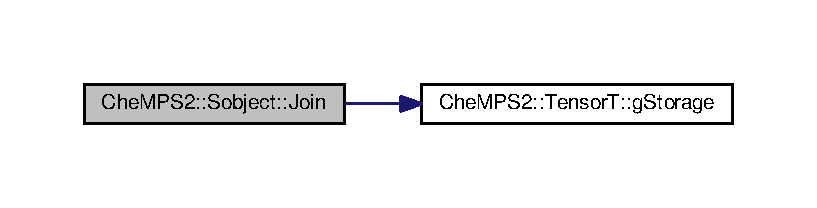
\includegraphics[width=350pt]{classCheMPS2_1_1Sobject_a687a29eab89ef3763af8c630b48e3bf6_cgraph}
\end{center}
\end{figure}




Here is the caller graph for this function\-:\nopagebreak
\begin{figure}[H]
\begin{center}
\leavevmode
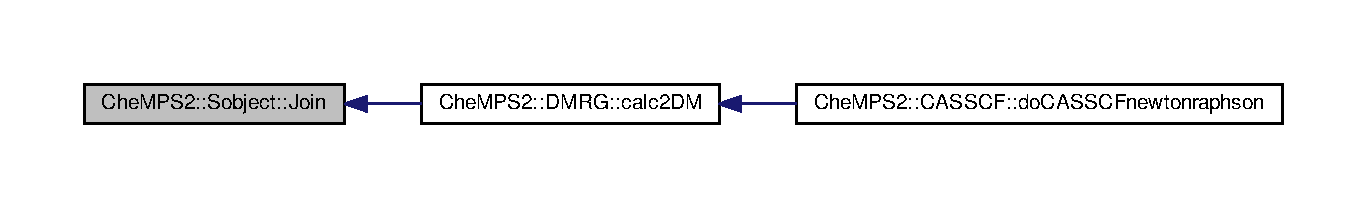
\includegraphics[width=350pt]{classCheMPS2_1_1Sobject_a687a29eab89ef3763af8c630b48e3bf6_icgraph}
\end{center}
\end{figure}


\hypertarget{classCheMPS2_1_1Sobject_a34983e86ae9f19de0be6b923479c13df}{\index{Che\-M\-P\-S2\-::\-Sobject@{Che\-M\-P\-S2\-::\-Sobject}!Split@{Split}}
\index{Split@{Split}!CheMPS2::Sobject@{Che\-M\-P\-S2\-::\-Sobject}}
\paragraph[{Split}]{\setlength{\rightskip}{0pt plus 5cm}double Che\-M\-P\-S2\-::\-Sobject\-::\-Split (
\begin{DoxyParamCaption}
\item[{{\bf Tensor\-T} $\ast$}]{Tleft, }
\item[{{\bf Tensor\-T} $\ast$}]{Tright, }
\item[{const int}]{virtualdimension\-D, }
\item[{const bool}]{movingright, }
\item[{const bool}]{change}
\end{DoxyParamCaption}
)}}\label{classCheMPS2_1_1Sobject_a34983e86ae9f19de0be6b923479c13df}


S\-V\-D an S-\/object into 2 \hyperlink{classCheMPS2_1_1TensorT}{Tensor\-T}'s. 


\begin{DoxyParams}{Parameters}
{\em Tleft} & Left \hyperlink{classCheMPS2_1_1TensorT}{Tensor\-T} storage space. At output left normalized. \\
\hline
{\em Tright} & Right \hyperlink{classCheMPS2_1_1TensorT}{Tensor\-T} storage space. At output right normalized. \\
\hline
{\em virtualdimension\-D} & The virtual dimension which is partitioned over the different symmetry blocks based on the Schmidt spectrum \\
\hline
{\em movingright} & When true, the singular values are multiplied into V$^\wedge$\-T, when false, into U. \\
\hline
{\em change} & Whether or not the symmetry virtual dimensions are allowed to change (when false\-: D doesn't matter) \\
\hline
\end{DoxyParams}
\begin{DoxyReturn}{Returns}
the discarded weight if change==true ; else 0.\-0 
\end{DoxyReturn}


Definition at line 233 of file Sobject.\-cpp.



Here is the call graph for this function\-:\nopagebreak
\begin{figure}[H]
\begin{center}
\leavevmode
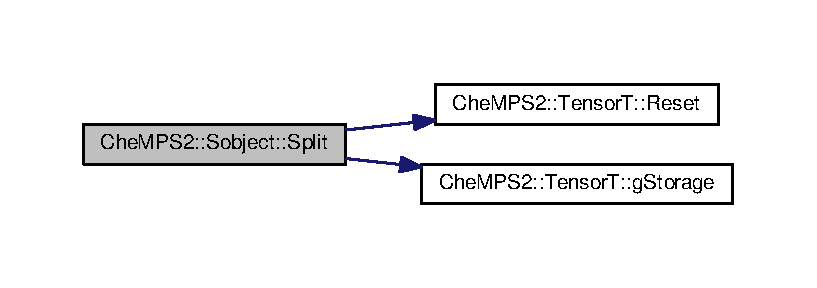
\includegraphics[width=350pt]{classCheMPS2_1_1Sobject_a34983e86ae9f19de0be6b923479c13df_cgraph}
\end{center}
\end{figure}




Here is the caller graph for this function\-:\nopagebreak
\begin{figure}[H]
\begin{center}
\leavevmode
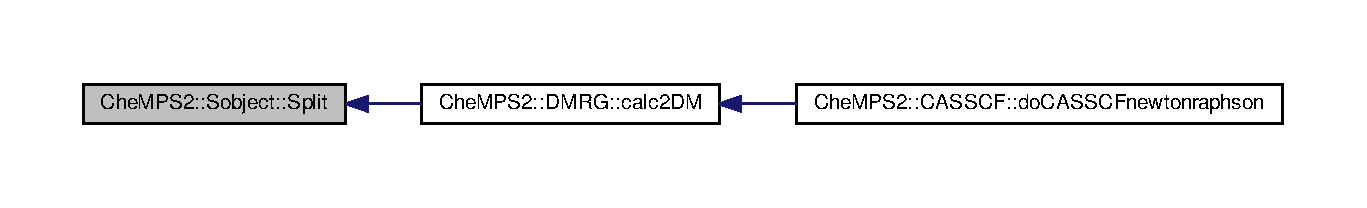
\includegraphics[width=350pt]{classCheMPS2_1_1Sobject_a34983e86ae9f19de0be6b923479c13df_icgraph}
\end{center}
\end{figure}




The documentation for this class was generated from the following files\-:\begin{DoxyCompactItemize}
\item 
Sobject.\-h\item 
Sobject.\-cpp\end{DoxyCompactItemize}

\hypertarget{classCheMPS2_1_1SyBookkeeper}{\subsection{Che\-M\-P\-S2\-:\-:Sy\-Bookkeeper Class Reference}
\label{classCheMPS2_1_1SyBookkeeper}\index{Che\-M\-P\-S2\-::\-Sy\-Bookkeeper@{Che\-M\-P\-S2\-::\-Sy\-Bookkeeper}}
}


{\ttfamily \#include $<$Sy\-Bookkeeper.\-h$>$}



Inheritance diagram for Che\-M\-P\-S2\-:\-:Sy\-Bookkeeper\-:\nopagebreak
\begin{figure}[H]
\begin{center}
\leavevmode
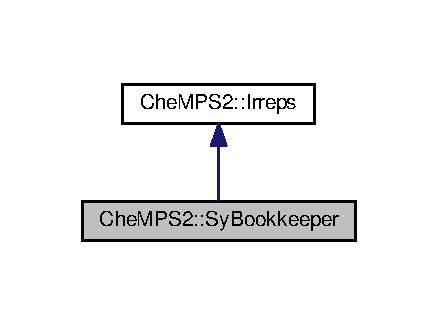
\includegraphics[width=210pt]{classCheMPS2_1_1SyBookkeeper__inherit__graph}
\end{center}
\end{figure}


Collaboration diagram for Che\-M\-P\-S2\-:\-:Sy\-Bookkeeper\-:\nopagebreak
\begin{figure}[H]
\begin{center}
\leavevmode
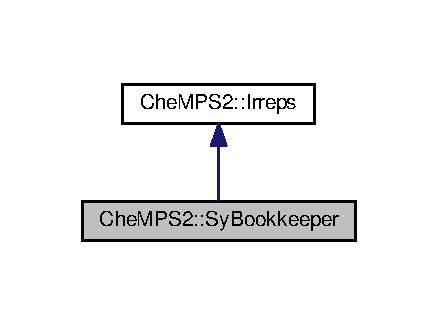
\includegraphics[width=210pt]{classCheMPS2_1_1SyBookkeeper__coll__graph}
\end{center}
\end{figure}
\subsubsection*{Public Member Functions}
\begin{DoxyCompactItemize}
\item 
\hyperlink{classCheMPS2_1_1SyBookkeeper_a755ef2a2c237dcacba3ac4a5a8ea272a}{Sy\-Bookkeeper} (const \hyperlink{classCheMPS2_1_1Problem}{Problem} $\ast$Probin, const int Din)
\begin{DoxyCompactList}\small\item\em Constructor. \end{DoxyCompactList}\item 
\hypertarget{classCheMPS2_1_1SyBookkeeper_a3904b642db40bc33db72612d3c534f8f}{\hyperlink{classCheMPS2_1_1SyBookkeeper_a3904b642db40bc33db72612d3c534f8f}{$\sim$\-Sy\-Bookkeeper} ()}\label{classCheMPS2_1_1SyBookkeeper_a3904b642db40bc33db72612d3c534f8f}

\begin{DoxyCompactList}\small\item\em Destructor. \end{DoxyCompactList}\item 
int \hyperlink{classCheMPS2_1_1SyBookkeeper_aff6ffb8d891d6380a7b2770348a0dcd7}{g\-L} () const 
\begin{DoxyCompactList}\small\item\em Get the number of orbitals. \end{DoxyCompactList}\item 
int \hyperlink{classCheMPS2_1_1SyBookkeeper_ab06fa32f4e352d248ebfe67d850a574a}{g\-Irrep} (const int n\-Orb) const 
\begin{DoxyCompactList}\small\item\em Get an orbital irrep. \end{DoxyCompactList}\item 
int \hyperlink{classCheMPS2_1_1SyBookkeeper_a72189d68fe5a90d9b5e4f11aa752a393}{g\-Two\-S} () const 
\begin{DoxyCompactList}\small\item\em Get twice the targeted spin. \end{DoxyCompactList}\item 
int \hyperlink{classCheMPS2_1_1SyBookkeeper_af39babd5df4cb5eeb84ffc017af841c3}{g\-N} () const 
\begin{DoxyCompactList}\small\item\em Get the targeted particle number. \end{DoxyCompactList}\item 
int \hyperlink{classCheMPS2_1_1SyBookkeeper_a280917b55df99e07e707f7e088b5f58d}{g\-Irrep} () const 
\begin{DoxyCompactList}\small\item\em Get the targeted irrep. \end{DoxyCompactList}\item 
int \hyperlink{classCheMPS2_1_1SyBookkeeper_a00b1b29641aade9ff5f4ce68e46c8320}{g\-Nmin} (const int bound) const 
\begin{DoxyCompactList}\small\item\em Get the min. possible particle number for a certain boundary. \end{DoxyCompactList}\item 
int \hyperlink{classCheMPS2_1_1SyBookkeeper_a39bc51595360d808a224ca6021ead99b}{g\-Nmax} (const int bound) const 
\begin{DoxyCompactList}\small\item\em Get the max. possible particle number for a certain boundary. \end{DoxyCompactList}\item 
int \hyperlink{classCheMPS2_1_1SyBookkeeper_aa1a9f3397c15a44e10035f22161fc825}{g\-Two\-Smin} (const int bound, const int N) const 
\begin{DoxyCompactList}\small\item\em Get the min. possible spin value for a certain boundary and particle number. \end{DoxyCompactList}\item 
int \hyperlink{classCheMPS2_1_1SyBookkeeper_a5203e4ac44a9c369974d9f817f634ddb}{g\-Two\-Smax} (const int bound, const int N) const 
\begin{DoxyCompactList}\small\item\em Get the max. possible spin value for a certain boundary and particle number. \end{DoxyCompactList}\item 
int \hyperlink{classCheMPS2_1_1SyBookkeeper_a6f5e333529c89f6f5f2ce2f11e082c49}{g\-F\-C\-Idim} (const int bound, const int N, const int Two\-S, const int Icnt) const 
\begin{DoxyCompactList}\small\item\em Get the F\-C\-I virtual dimensions (bound by cutoff) \end{DoxyCompactList}\item 
int \hyperlink{classCheMPS2_1_1SyBookkeeper_a44ff8a4f047febaab0674a239c982715}{g\-D} () const 
\begin{DoxyCompactList}\small\item\em Get the total (reduced) virtual dimension. \end{DoxyCompactList}\item 
int \hyperlink{classCheMPS2_1_1SyBookkeeper_ab9e13e1079e56b1ee12d4ed82b8c7d82}{g\-Current\-Dim} (const int bound, const int N, const int Two\-S, const int Icnt) const 
\begin{DoxyCompactList}\small\item\em Get the current virtual dimensions. \end{DoxyCompactList}\item 
bool \hyperlink{classCheMPS2_1_1SyBookkeeper_ae6bcbf2398cda17b45c02af73a02fc65}{Is\-Possible} () const 
\begin{DoxyCompactList}\small\item\em Get whether the desired symmetry sector is possible. \end{DoxyCompactList}\item 
void \hyperlink{classCheMPS2_1_1SyBookkeeper_ab496351a4cbc31f88be340d987d11406}{Set\-Dim} (const int bound, const int N, const int Two\-S, const int Icnt, const int val)
\begin{DoxyCompactList}\small\item\em Get the current virtual dimensions. \end{DoxyCompactList}\item 
int \hyperlink{classCheMPS2_1_1SyBookkeeper_ad52f6f852f6f2f88c286579054c1886f}{g\-Max\-Dim\-At\-Bound} (const int i\-Bound) const 
\begin{DoxyCompactList}\small\item\em Get the max. virtual dimension at a certain boundary. Useful function to preallocate memory when constructing \hyperlink{classCheMPS2_1_1Heff}{Heff}. \end{DoxyCompactList}\end{DoxyCompactItemize}
\subsubsection*{Additional Inherited Members}


\subsubsection{Detailed Description}
\hyperlink{classCheMPS2_1_1SyBookkeeper}{Sy\-Bookkeeper} class. \begin{DoxyAuthor}{Author}
Sebastian Wouters \href{mailto:sebastianwouters@gmail.com}{\tt sebastianwouters@gmail.\-com} 
\end{DoxyAuthor}
\begin{DoxyDate}{Date}
February 14, 2013
\end{DoxyDate}
The \hyperlink{classCheMPS2_1_1SyBookkeeper}{Sy\-Bookkeeper} class keeps track of all the symmetry at the boundaries. This includes\-:
\begin{DoxyItemize}
\item the F\-C\-I virtual dimensions per symmetry sector
\item an extra consistency check (next to the one in \hyperlink{Problem_8cpp_source}{Problem.\-cpp}) to check whether the desired symmetry in the \hyperlink{classCheMPS2_1_1Problem}{Problem} class is possible (non-\/zero F\-C\-I dimensions)
\item the current virtual dimensions per symmetry sector, so everyone can check the current dimensions here. 
\end{DoxyItemize}

Definition at line 36 of file Sy\-Bookkeeper.\-h.



\subsubsection{Constructor \& Destructor Documentation}
\hypertarget{classCheMPS2_1_1SyBookkeeper_a755ef2a2c237dcacba3ac4a5a8ea272a}{\index{Che\-M\-P\-S2\-::\-Sy\-Bookkeeper@{Che\-M\-P\-S2\-::\-Sy\-Bookkeeper}!Sy\-Bookkeeper@{Sy\-Bookkeeper}}
\index{Sy\-Bookkeeper@{Sy\-Bookkeeper}!CheMPS2::SyBookkeeper@{Che\-M\-P\-S2\-::\-Sy\-Bookkeeper}}
\paragraph[{Sy\-Bookkeeper}]{\setlength{\rightskip}{0pt plus 5cm}Che\-M\-P\-S2\-::\-Sy\-Bookkeeper\-::\-Sy\-Bookkeeper (
\begin{DoxyParamCaption}
\item[{const {\bf Problem} $\ast$}]{Probin, }
\item[{const int}]{Din}
\end{DoxyParamCaption}
)}}\label{classCheMPS2_1_1SyBookkeeper_a755ef2a2c237dcacba3ac4a5a8ea272a}


Constructor. 


\begin{DoxyParams}{Parameters}
{\em Probin} & The problem to be solved \\
\hline
{\em Din} & The initial number of reduced renormalized \hyperlink{classCheMPS2_1_1DMRG}{D\-M\-R\-G} basis states \\
\hline
\end{DoxyParams}


Definition at line 32 of file Sy\-Bookkeeper.\-cpp.



Here is the call graph for this function\-:\nopagebreak
\begin{figure}[H]
\begin{center}
\leavevmode
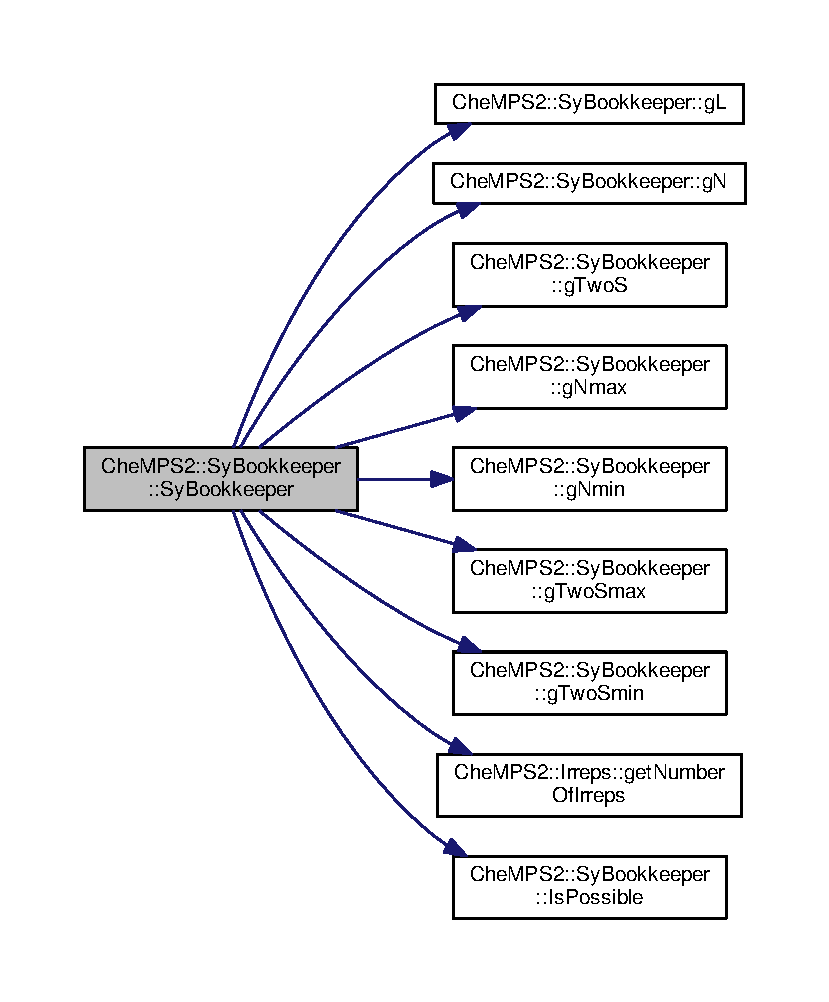
\includegraphics[width=350pt]{classCheMPS2_1_1SyBookkeeper_a755ef2a2c237dcacba3ac4a5a8ea272a_cgraph}
\end{center}
\end{figure}




\subsubsection{Member Function Documentation}
\hypertarget{classCheMPS2_1_1SyBookkeeper_ab9e13e1079e56b1ee12d4ed82b8c7d82}{\index{Che\-M\-P\-S2\-::\-Sy\-Bookkeeper@{Che\-M\-P\-S2\-::\-Sy\-Bookkeeper}!g\-Current\-Dim@{g\-Current\-Dim}}
\index{g\-Current\-Dim@{g\-Current\-Dim}!CheMPS2::SyBookkeeper@{Che\-M\-P\-S2\-::\-Sy\-Bookkeeper}}
\paragraph[{g\-Current\-Dim}]{\setlength{\rightskip}{0pt plus 5cm}int Che\-M\-P\-S2\-::\-Sy\-Bookkeeper\-::g\-Current\-Dim (
\begin{DoxyParamCaption}
\item[{const int}]{bound, }
\item[{const int}]{N, }
\item[{const int}]{Two\-S, }
\item[{const int}]{Icnt}
\end{DoxyParamCaption}
) const}}\label{classCheMPS2_1_1SyBookkeeper_ab9e13e1079e56b1ee12d4ed82b8c7d82}


Get the current virtual dimensions. 


\begin{DoxyParams}{Parameters}
{\em bound} & The boundary index \\
\hline
{\em N} & The particle number \\
\hline
{\em Two\-S} & Twice the spin sector \\
\hline
{\em Icnt} & The irrep \\
\hline
\end{DoxyParams}
\begin{DoxyReturn}{Returns}
Current\-Dim\mbox{[}bound\mbox{]}\mbox{[}N-\/g\-Nmin(bound)\mbox{]}\mbox{[}(Two\-S-\/g\-Two\-Smin(bound,N))/2\mbox{]}\mbox{[}Icnt\mbox{]} 
\end{DoxyReturn}


Definition at line 127 of file Sy\-Bookkeeper.\-cpp.



Here is the caller graph for this function\-:\nopagebreak
\begin{figure}[H]
\begin{center}
\leavevmode
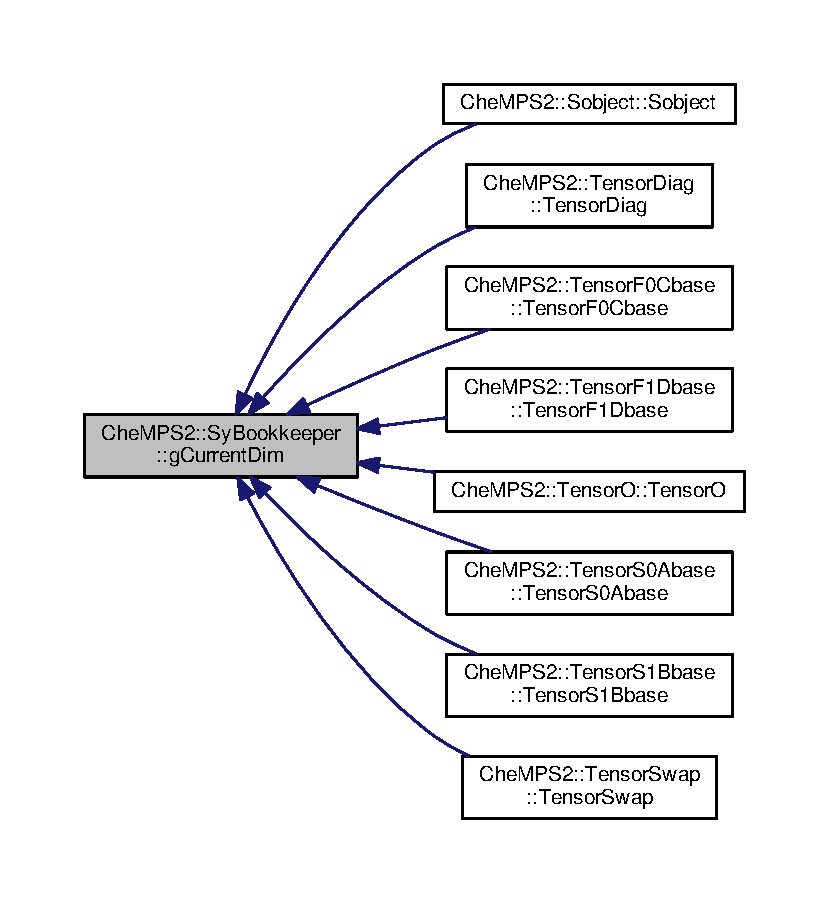
\includegraphics[width=350pt]{classCheMPS2_1_1SyBookkeeper_ab9e13e1079e56b1ee12d4ed82b8c7d82_icgraph}
\end{center}
\end{figure}


\hypertarget{classCheMPS2_1_1SyBookkeeper_a44ff8a4f047febaab0674a239c982715}{\index{Che\-M\-P\-S2\-::\-Sy\-Bookkeeper@{Che\-M\-P\-S2\-::\-Sy\-Bookkeeper}!g\-D@{g\-D}}
\index{g\-D@{g\-D}!CheMPS2::SyBookkeeper@{Che\-M\-P\-S2\-::\-Sy\-Bookkeeper}}
\paragraph[{g\-D}]{\setlength{\rightskip}{0pt plus 5cm}int Che\-M\-P\-S2\-::\-Sy\-Bookkeeper\-::g\-D (
\begin{DoxyParamCaption}
{}
\end{DoxyParamCaption}
) const}}\label{classCheMPS2_1_1SyBookkeeper_a44ff8a4f047febaab0674a239c982715}


Get the total (reduced) virtual dimension. 

\begin{DoxyReturn}{Returns}
The virtual dimension (reduced) 
\end{DoxyReturn}
\hypertarget{classCheMPS2_1_1SyBookkeeper_a6f5e333529c89f6f5f2ce2f11e082c49}{\index{Che\-M\-P\-S2\-::\-Sy\-Bookkeeper@{Che\-M\-P\-S2\-::\-Sy\-Bookkeeper}!g\-F\-C\-Idim@{g\-F\-C\-Idim}}
\index{g\-F\-C\-Idim@{g\-F\-C\-Idim}!CheMPS2::SyBookkeeper@{Che\-M\-P\-S2\-::\-Sy\-Bookkeeper}}
\paragraph[{g\-F\-C\-Idim}]{\setlength{\rightskip}{0pt plus 5cm}int Che\-M\-P\-S2\-::\-Sy\-Bookkeeper\-::g\-F\-C\-Idim (
\begin{DoxyParamCaption}
\item[{const int}]{bound, }
\item[{const int}]{N, }
\item[{const int}]{Two\-S, }
\item[{const int}]{Icnt}
\end{DoxyParamCaption}
) const}}\label{classCheMPS2_1_1SyBookkeeper_a6f5e333529c89f6f5f2ce2f11e082c49}


Get the F\-C\-I virtual dimensions (bound by cutoff) 


\begin{DoxyParams}{Parameters}
{\em bound} & The boundary index \\
\hline
{\em N} & The particle number \\
\hline
{\em Two\-S} & Twice the spin sector \\
\hline
{\em Icnt} & The irrep \\
\hline
\end{DoxyParams}
\begin{DoxyReturn}{Returns}
F\-C\-Idim\mbox{[}bound\mbox{]}\mbox{[}N-\/g\-Nmin(bound)\mbox{]}\mbox{[}(Two\-S-\/g\-Two\-Smin(bound,N))/2\mbox{]}\mbox{[}Icnt\mbox{]} 
\end{DoxyReturn}


Definition at line 125 of file Sy\-Bookkeeper.\-cpp.

\hypertarget{classCheMPS2_1_1SyBookkeeper_ab06fa32f4e352d248ebfe67d850a574a}{\index{Che\-M\-P\-S2\-::\-Sy\-Bookkeeper@{Che\-M\-P\-S2\-::\-Sy\-Bookkeeper}!g\-Irrep@{g\-Irrep}}
\index{g\-Irrep@{g\-Irrep}!CheMPS2::SyBookkeeper@{Che\-M\-P\-S2\-::\-Sy\-Bookkeeper}}
\paragraph[{g\-Irrep}]{\setlength{\rightskip}{0pt plus 5cm}int Che\-M\-P\-S2\-::\-Sy\-Bookkeeper\-::g\-Irrep (
\begin{DoxyParamCaption}
\item[{const int}]{n\-Orb}
\end{DoxyParamCaption}
) const}}\label{classCheMPS2_1_1SyBookkeeper_ab06fa32f4e352d248ebfe67d850a574a}


Get an orbital irrep. 


\begin{DoxyParams}{Parameters}
{\em n\-Orb} & The orbital index \\
\hline
\end{DoxyParams}
\begin{DoxyReturn}{Returns}
The irrep of the orbital with index n\-Orb 
\end{DoxyReturn}


Definition at line 109 of file Sy\-Bookkeeper.\-cpp.



Here is the caller graph for this function\-:\nopagebreak
\begin{figure}[H]
\begin{center}
\leavevmode
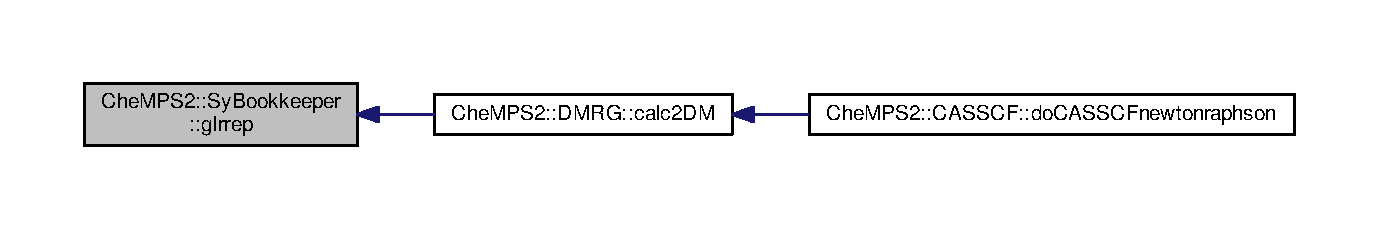
\includegraphics[width=350pt]{classCheMPS2_1_1SyBookkeeper_ab06fa32f4e352d248ebfe67d850a574a_icgraph}
\end{center}
\end{figure}


\hypertarget{classCheMPS2_1_1SyBookkeeper_a280917b55df99e07e707f7e088b5f58d}{\index{Che\-M\-P\-S2\-::\-Sy\-Bookkeeper@{Che\-M\-P\-S2\-::\-Sy\-Bookkeeper}!g\-Irrep@{g\-Irrep}}
\index{g\-Irrep@{g\-Irrep}!CheMPS2::SyBookkeeper@{Che\-M\-P\-S2\-::\-Sy\-Bookkeeper}}
\paragraph[{g\-Irrep}]{\setlength{\rightskip}{0pt plus 5cm}int Che\-M\-P\-S2\-::\-Sy\-Bookkeeper\-::g\-Irrep (
\begin{DoxyParamCaption}
{}
\end{DoxyParamCaption}
) const}}\label{classCheMPS2_1_1SyBookkeeper_a280917b55df99e07e707f7e088b5f58d}


Get the targeted irrep. 

\begin{DoxyReturn}{Returns}
The targeted irrep 
\end{DoxyReturn}


Definition at line 115 of file Sy\-Bookkeeper.\-cpp.

\hypertarget{classCheMPS2_1_1SyBookkeeper_aff6ffb8d891d6380a7b2770348a0dcd7}{\index{Che\-M\-P\-S2\-::\-Sy\-Bookkeeper@{Che\-M\-P\-S2\-::\-Sy\-Bookkeeper}!g\-L@{g\-L}}
\index{g\-L@{g\-L}!CheMPS2::SyBookkeeper@{Che\-M\-P\-S2\-::\-Sy\-Bookkeeper}}
\paragraph[{g\-L}]{\setlength{\rightskip}{0pt plus 5cm}int Che\-M\-P\-S2\-::\-Sy\-Bookkeeper\-::g\-L (
\begin{DoxyParamCaption}
{}
\end{DoxyParamCaption}
) const}}\label{classCheMPS2_1_1SyBookkeeper_aff6ffb8d891d6380a7b2770348a0dcd7}


Get the number of orbitals. 

\begin{DoxyReturn}{Returns}
The number of orbitals 
\end{DoxyReturn}


Definition at line 107 of file Sy\-Bookkeeper.\-cpp.



Here is the caller graph for this function\-:\nopagebreak
\begin{figure}[H]
\begin{center}
\leavevmode
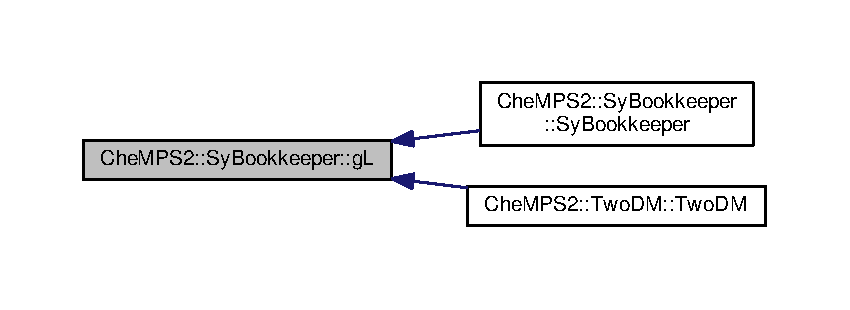
\includegraphics[width=350pt]{classCheMPS2_1_1SyBookkeeper_aff6ffb8d891d6380a7b2770348a0dcd7_icgraph}
\end{center}
\end{figure}


\hypertarget{classCheMPS2_1_1SyBookkeeper_ad52f6f852f6f2f88c286579054c1886f}{\index{Che\-M\-P\-S2\-::\-Sy\-Bookkeeper@{Che\-M\-P\-S2\-::\-Sy\-Bookkeeper}!g\-Max\-Dim\-At\-Bound@{g\-Max\-Dim\-At\-Bound}}
\index{g\-Max\-Dim\-At\-Bound@{g\-Max\-Dim\-At\-Bound}!CheMPS2::SyBookkeeper@{Che\-M\-P\-S2\-::\-Sy\-Bookkeeper}}
\paragraph[{g\-Max\-Dim\-At\-Bound}]{\setlength{\rightskip}{0pt plus 5cm}int Che\-M\-P\-S2\-::\-Sy\-Bookkeeper\-::g\-Max\-Dim\-At\-Bound (
\begin{DoxyParamCaption}
\item[{const int}]{i\-Bound}
\end{DoxyParamCaption}
) const}}\label{classCheMPS2_1_1SyBookkeeper_ad52f6f852f6f2f88c286579054c1886f}


Get the max. virtual dimension at a certain boundary. Useful function to preallocate memory when constructing \hyperlink{classCheMPS2_1_1Heff}{Heff}. 


\begin{DoxyParams}{Parameters}
{\em i\-Bound} & The boundary index \\
\hline
\end{DoxyParams}
\begin{DoxyReturn}{Returns}
The max. virtual dimension at i\-Bound 
\end{DoxyReturn}


Definition at line 272 of file Sy\-Bookkeeper.\-cpp.

\hypertarget{classCheMPS2_1_1SyBookkeeper_af39babd5df4cb5eeb84ffc017af841c3}{\index{Che\-M\-P\-S2\-::\-Sy\-Bookkeeper@{Che\-M\-P\-S2\-::\-Sy\-Bookkeeper}!g\-N@{g\-N}}
\index{g\-N@{g\-N}!CheMPS2::SyBookkeeper@{Che\-M\-P\-S2\-::\-Sy\-Bookkeeper}}
\paragraph[{g\-N}]{\setlength{\rightskip}{0pt plus 5cm}int Che\-M\-P\-S2\-::\-Sy\-Bookkeeper\-::g\-N (
\begin{DoxyParamCaption}
{}
\end{DoxyParamCaption}
) const}}\label{classCheMPS2_1_1SyBookkeeper_af39babd5df4cb5eeb84ffc017af841c3}


Get the targeted particle number. 

\begin{DoxyReturn}{Returns}
The targeted particle number 
\end{DoxyReturn}


Definition at line 113 of file Sy\-Bookkeeper.\-cpp.



Here is the caller graph for this function\-:\nopagebreak
\begin{figure}[H]
\begin{center}
\leavevmode
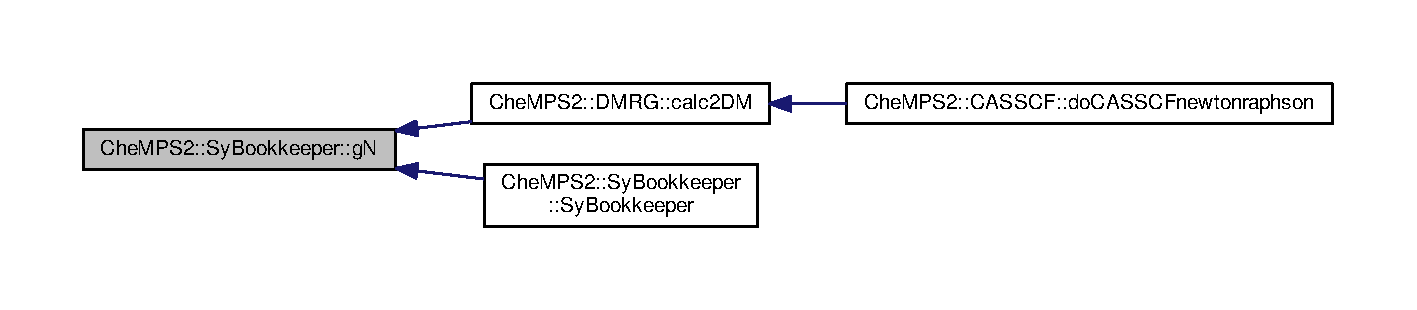
\includegraphics[width=350pt]{classCheMPS2_1_1SyBookkeeper_af39babd5df4cb5eeb84ffc017af841c3_icgraph}
\end{center}
\end{figure}


\hypertarget{classCheMPS2_1_1SyBookkeeper_a39bc51595360d808a224ca6021ead99b}{\index{Che\-M\-P\-S2\-::\-Sy\-Bookkeeper@{Che\-M\-P\-S2\-::\-Sy\-Bookkeeper}!g\-Nmax@{g\-Nmax}}
\index{g\-Nmax@{g\-Nmax}!CheMPS2::SyBookkeeper@{Che\-M\-P\-S2\-::\-Sy\-Bookkeeper}}
\paragraph[{g\-Nmax}]{\setlength{\rightskip}{0pt plus 5cm}int Che\-M\-P\-S2\-::\-Sy\-Bookkeeper\-::g\-Nmax (
\begin{DoxyParamCaption}
\item[{const int}]{bound}
\end{DoxyParamCaption}
) const}}\label{classCheMPS2_1_1SyBookkeeper_a39bc51595360d808a224ca6021ead99b}


Get the max. possible particle number for a certain boundary. 


\begin{DoxyParams}{Parameters}
{\em bound} & The boundary index \\
\hline
\end{DoxyParams}
\begin{DoxyReturn}{Returns}
Nmax\mbox{[}bound\mbox{]} 
\end{DoxyReturn}


Definition at line 119 of file Sy\-Bookkeeper.\-cpp.



Here is the caller graph for this function\-:\nopagebreak
\begin{figure}[H]
\begin{center}
\leavevmode
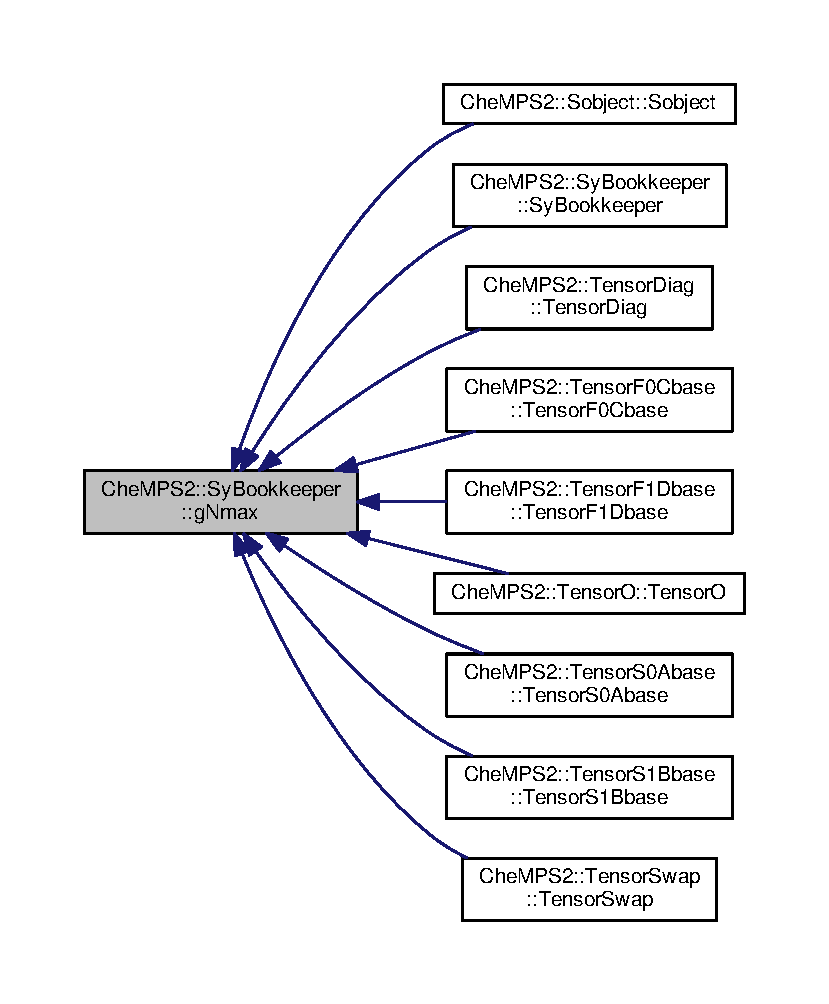
\includegraphics[width=350pt]{classCheMPS2_1_1SyBookkeeper_a39bc51595360d808a224ca6021ead99b_icgraph}
\end{center}
\end{figure}


\hypertarget{classCheMPS2_1_1SyBookkeeper_a00b1b29641aade9ff5f4ce68e46c8320}{\index{Che\-M\-P\-S2\-::\-Sy\-Bookkeeper@{Che\-M\-P\-S2\-::\-Sy\-Bookkeeper}!g\-Nmin@{g\-Nmin}}
\index{g\-Nmin@{g\-Nmin}!CheMPS2::SyBookkeeper@{Che\-M\-P\-S2\-::\-Sy\-Bookkeeper}}
\paragraph[{g\-Nmin}]{\setlength{\rightskip}{0pt plus 5cm}int Che\-M\-P\-S2\-::\-Sy\-Bookkeeper\-::g\-Nmin (
\begin{DoxyParamCaption}
\item[{const int}]{bound}
\end{DoxyParamCaption}
) const}}\label{classCheMPS2_1_1SyBookkeeper_a00b1b29641aade9ff5f4ce68e46c8320}


Get the min. possible particle number for a certain boundary. 


\begin{DoxyParams}{Parameters}
{\em bound} & The boundary index (from 0 to L (included)) \\
\hline
\end{DoxyParams}
\begin{DoxyReturn}{Returns}
Nmin\mbox{[}bound\mbox{]} 
\end{DoxyReturn}


Definition at line 117 of file Sy\-Bookkeeper.\-cpp.



Here is the caller graph for this function\-:\nopagebreak
\begin{figure}[H]
\begin{center}
\leavevmode
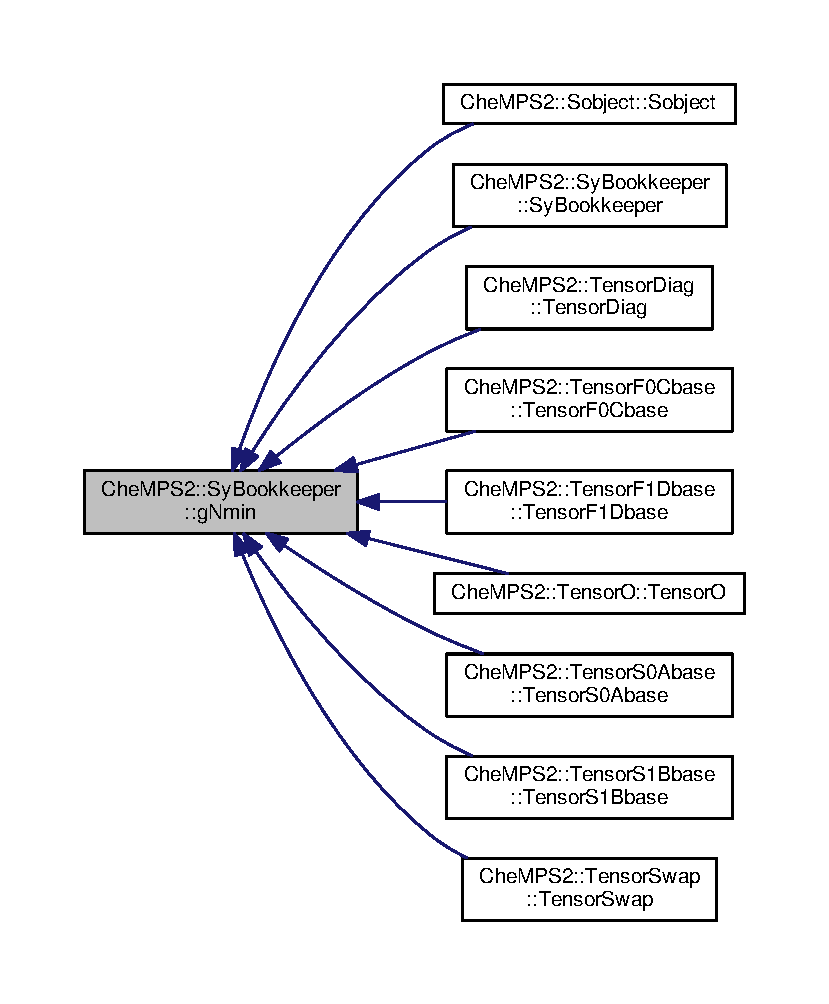
\includegraphics[width=350pt]{classCheMPS2_1_1SyBookkeeper_a00b1b29641aade9ff5f4ce68e46c8320_icgraph}
\end{center}
\end{figure}


\hypertarget{classCheMPS2_1_1SyBookkeeper_a72189d68fe5a90d9b5e4f11aa752a393}{\index{Che\-M\-P\-S2\-::\-Sy\-Bookkeeper@{Che\-M\-P\-S2\-::\-Sy\-Bookkeeper}!g\-Two\-S@{g\-Two\-S}}
\index{g\-Two\-S@{g\-Two\-S}!CheMPS2::SyBookkeeper@{Che\-M\-P\-S2\-::\-Sy\-Bookkeeper}}
\paragraph[{g\-Two\-S}]{\setlength{\rightskip}{0pt plus 5cm}int Che\-M\-P\-S2\-::\-Sy\-Bookkeeper\-::g\-Two\-S (
\begin{DoxyParamCaption}
{}
\end{DoxyParamCaption}
) const}}\label{classCheMPS2_1_1SyBookkeeper_a72189d68fe5a90d9b5e4f11aa752a393}


Get twice the targeted spin. 

\begin{DoxyReturn}{Returns}
Twice the targeted spin 
\end{DoxyReturn}


Definition at line 111 of file Sy\-Bookkeeper.\-cpp.



Here is the caller graph for this function\-:\nopagebreak
\begin{figure}[H]
\begin{center}
\leavevmode
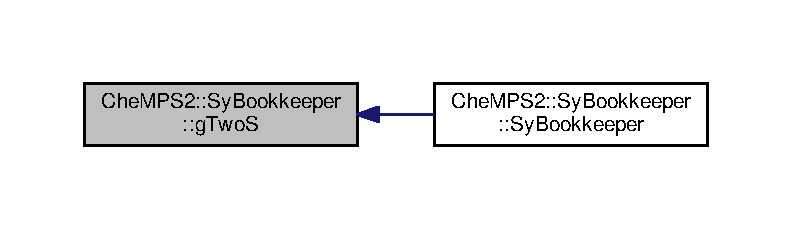
\includegraphics[width=350pt]{classCheMPS2_1_1SyBookkeeper_a72189d68fe5a90d9b5e4f11aa752a393_icgraph}
\end{center}
\end{figure}


\hypertarget{classCheMPS2_1_1SyBookkeeper_a5203e4ac44a9c369974d9f817f634ddb}{\index{Che\-M\-P\-S2\-::\-Sy\-Bookkeeper@{Che\-M\-P\-S2\-::\-Sy\-Bookkeeper}!g\-Two\-Smax@{g\-Two\-Smax}}
\index{g\-Two\-Smax@{g\-Two\-Smax}!CheMPS2::SyBookkeeper@{Che\-M\-P\-S2\-::\-Sy\-Bookkeeper}}
\paragraph[{g\-Two\-Smax}]{\setlength{\rightskip}{0pt plus 5cm}int Che\-M\-P\-S2\-::\-Sy\-Bookkeeper\-::g\-Two\-Smax (
\begin{DoxyParamCaption}
\item[{const int}]{bound, }
\item[{const int}]{N}
\end{DoxyParamCaption}
) const}}\label{classCheMPS2_1_1SyBookkeeper_a5203e4ac44a9c369974d9f817f634ddb}


Get the max. possible spin value for a certain boundary and particle number. 


\begin{DoxyParams}{Parameters}
{\em bound} & The boundary index \\
\hline
{\em N} & The particle number \\
\hline
\end{DoxyParams}
\begin{DoxyReturn}{Returns}
Two\-Smax\mbox{[}bound\mbox{]}\mbox{[}N-\/\-Nmin\mbox{[}bound\mbox{]}\mbox{]} 
\end{DoxyReturn}


Definition at line 123 of file Sy\-Bookkeeper.\-cpp.



Here is the caller graph for this function\-:\nopagebreak
\begin{figure}[H]
\begin{center}
\leavevmode
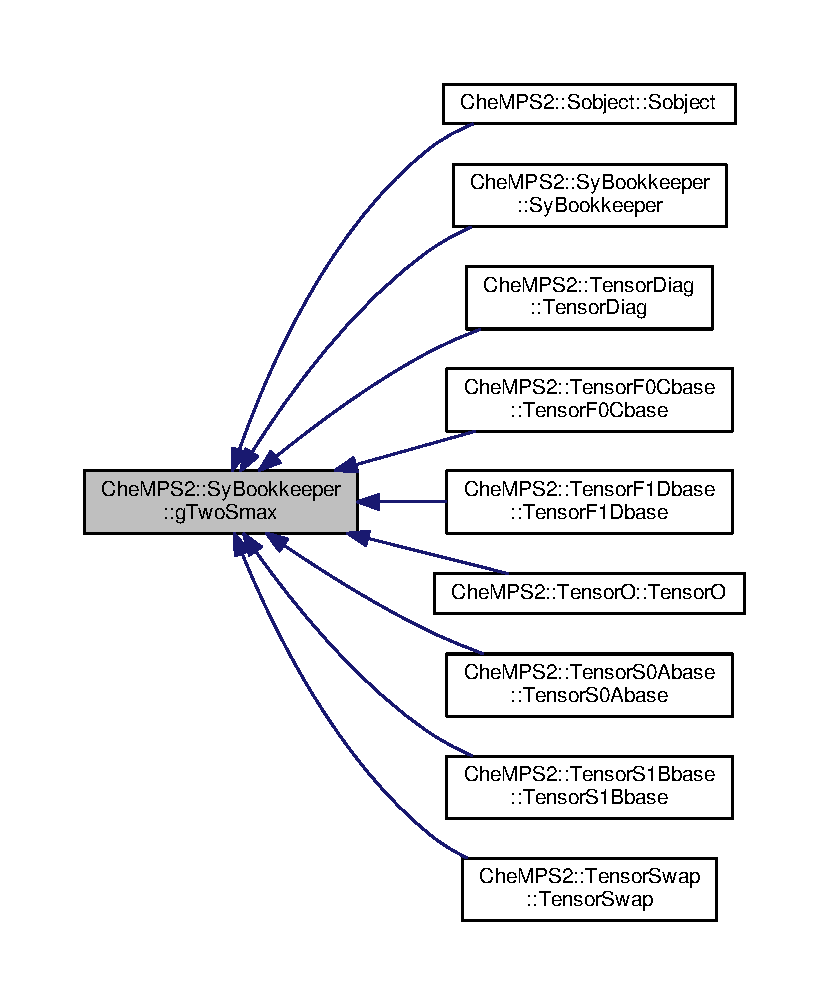
\includegraphics[width=350pt]{classCheMPS2_1_1SyBookkeeper_a5203e4ac44a9c369974d9f817f634ddb_icgraph}
\end{center}
\end{figure}


\hypertarget{classCheMPS2_1_1SyBookkeeper_aa1a9f3397c15a44e10035f22161fc825}{\index{Che\-M\-P\-S2\-::\-Sy\-Bookkeeper@{Che\-M\-P\-S2\-::\-Sy\-Bookkeeper}!g\-Two\-Smin@{g\-Two\-Smin}}
\index{g\-Two\-Smin@{g\-Two\-Smin}!CheMPS2::SyBookkeeper@{Che\-M\-P\-S2\-::\-Sy\-Bookkeeper}}
\paragraph[{g\-Two\-Smin}]{\setlength{\rightskip}{0pt plus 5cm}int Che\-M\-P\-S2\-::\-Sy\-Bookkeeper\-::g\-Two\-Smin (
\begin{DoxyParamCaption}
\item[{const int}]{bound, }
\item[{const int}]{N}
\end{DoxyParamCaption}
) const}}\label{classCheMPS2_1_1SyBookkeeper_aa1a9f3397c15a44e10035f22161fc825}


Get the min. possible spin value for a certain boundary and particle number. 


\begin{DoxyParams}{Parameters}
{\em bound} & The boundary index \\
\hline
{\em N} & The particle number \\
\hline
\end{DoxyParams}
\begin{DoxyReturn}{Returns}
Two\-Smin\mbox{[}bound\mbox{]}\mbox{[}N-\/\-Nmin\mbox{[}bound\mbox{]}\mbox{]} 
\end{DoxyReturn}


Definition at line 121 of file Sy\-Bookkeeper.\-cpp.



Here is the caller graph for this function\-:\nopagebreak
\begin{figure}[H]
\begin{center}
\leavevmode
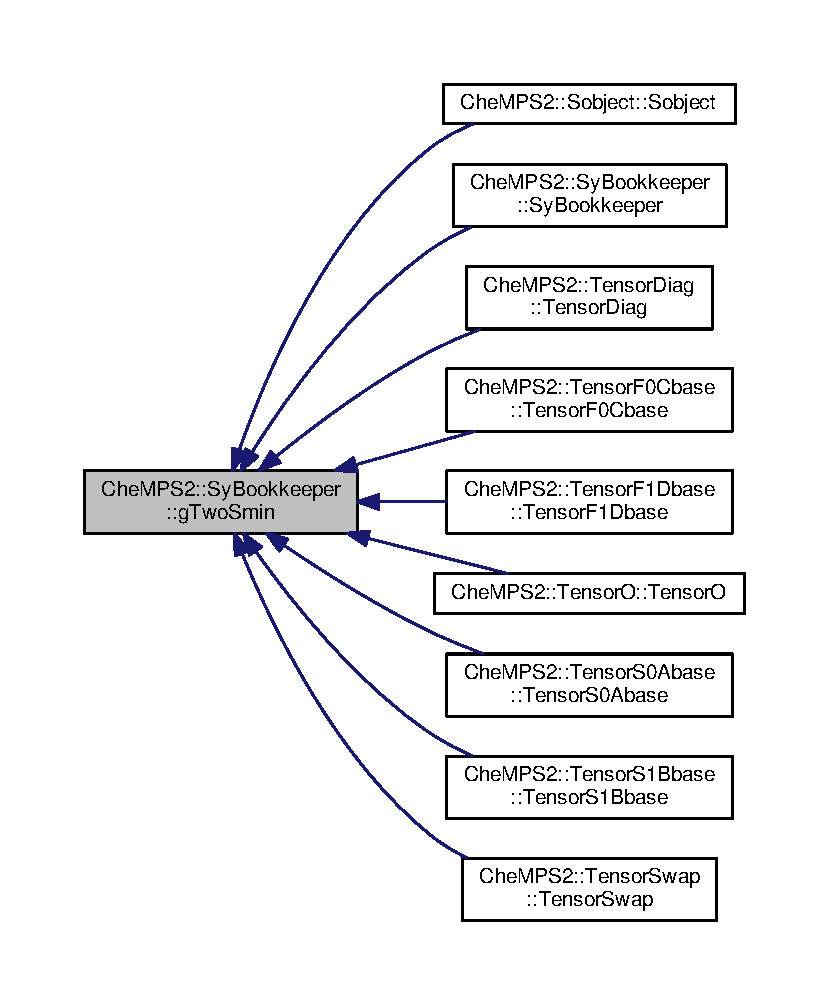
\includegraphics[width=350pt]{classCheMPS2_1_1SyBookkeeper_aa1a9f3397c15a44e10035f22161fc825_icgraph}
\end{center}
\end{figure}


\hypertarget{classCheMPS2_1_1SyBookkeeper_ae6bcbf2398cda17b45c02af73a02fc65}{\index{Che\-M\-P\-S2\-::\-Sy\-Bookkeeper@{Che\-M\-P\-S2\-::\-Sy\-Bookkeeper}!Is\-Possible@{Is\-Possible}}
\index{Is\-Possible@{Is\-Possible}!CheMPS2::SyBookkeeper@{Che\-M\-P\-S2\-::\-Sy\-Bookkeeper}}
\paragraph[{Is\-Possible}]{\setlength{\rightskip}{0pt plus 5cm}bool Che\-M\-P\-S2\-::\-Sy\-Bookkeeper\-::\-Is\-Possible (
\begin{DoxyParamCaption}
{}
\end{DoxyParamCaption}
) const}}\label{classCheMPS2_1_1SyBookkeeper_ae6bcbf2398cda17b45c02af73a02fc65}


Get whether the desired symmetry sector is possible. 

\begin{DoxyReturn}{Returns}
The virtual dimension (reduced) 
\end{DoxyReturn}


Definition at line 313 of file Sy\-Bookkeeper.\-cpp.



Here is the caller graph for this function\-:\nopagebreak
\begin{figure}[H]
\begin{center}
\leavevmode
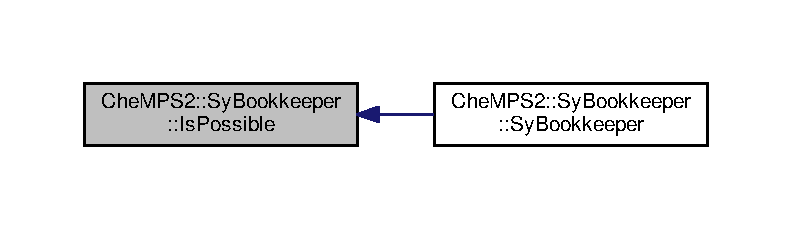
\includegraphics[width=350pt]{classCheMPS2_1_1SyBookkeeper_ae6bcbf2398cda17b45c02af73a02fc65_icgraph}
\end{center}
\end{figure}


\hypertarget{classCheMPS2_1_1SyBookkeeper_ab496351a4cbc31f88be340d987d11406}{\index{Che\-M\-P\-S2\-::\-Sy\-Bookkeeper@{Che\-M\-P\-S2\-::\-Sy\-Bookkeeper}!Set\-Dim@{Set\-Dim}}
\index{Set\-Dim@{Set\-Dim}!CheMPS2::SyBookkeeper@{Che\-M\-P\-S2\-::\-Sy\-Bookkeeper}}
\paragraph[{Set\-Dim}]{\setlength{\rightskip}{0pt plus 5cm}void Che\-M\-P\-S2\-::\-Sy\-Bookkeeper\-::\-Set\-Dim (
\begin{DoxyParamCaption}
\item[{const int}]{bound, }
\item[{const int}]{N, }
\item[{const int}]{Two\-S, }
\item[{const int}]{Icnt, }
\item[{const int}]{val}
\end{DoxyParamCaption}
)}}\label{classCheMPS2_1_1SyBookkeeper_ab496351a4cbc31f88be340d987d11406}


Get the current virtual dimensions. 


\begin{DoxyParams}{Parameters}
{\em bound} & The boundary index \\
\hline
{\em N} & The particle number \\
\hline
{\em Two\-S} & Twice the spin sector \\
\hline
{\em Icnt} & The irrep \\
\hline
{\em val} & The new dimension size \\
\hline
\end{DoxyParams}


Definition at line 129 of file Sy\-Bookkeeper.\-cpp.



The documentation for this class was generated from the following files\-:\begin{DoxyCompactItemize}
\item 
Sy\-Bookkeeper.\-h\item 
Sy\-Bookkeeper.\-cpp\end{DoxyCompactItemize}

\hypertarget{classCheMPS2_1_1Tensor}{\subsection{Che\-M\-P\-S2\-:\-:Tensor Class Reference}
\label{classCheMPS2_1_1Tensor}\index{Che\-M\-P\-S2\-::\-Tensor@{Che\-M\-P\-S2\-::\-Tensor}}
}


{\ttfamily \#include $<$Tensor.\-h$>$}



Inheritance diagram for Che\-M\-P\-S2\-:\-:Tensor\-:\nopagebreak
\begin{figure}[H]
\begin{center}
\leavevmode
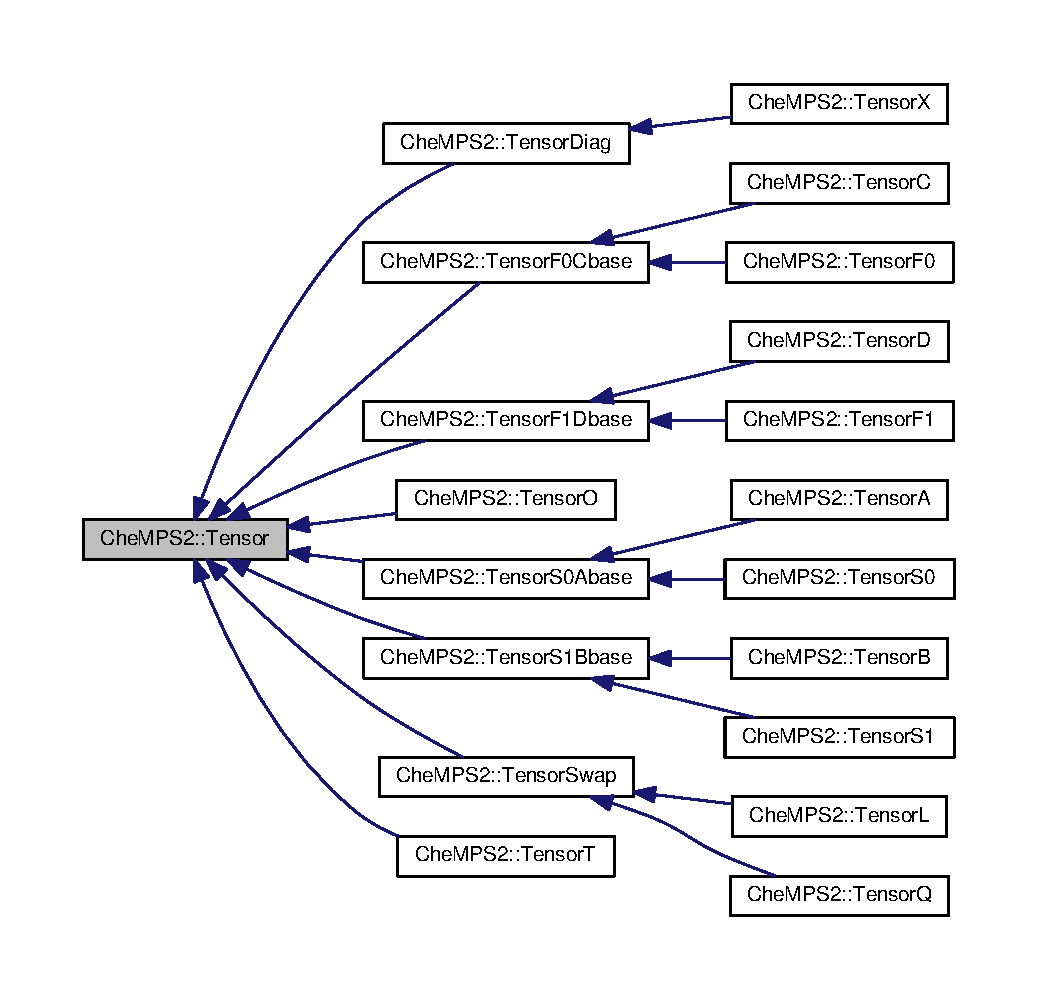
\includegraphics[width=350pt]{classCheMPS2_1_1Tensor__inherit__graph}
\end{center}
\end{figure}


Collaboration diagram for Che\-M\-P\-S2\-:\-:Tensor\-:\nopagebreak
\begin{figure}[H]
\begin{center}
\leavevmode
\includegraphics[width=210pt]{classCheMPS2_1_1Tensor__coll__graph}
\end{center}
\end{figure}
\subsubsection*{Public Member Functions}
\begin{DoxyCompactItemize}
\item 
virtual int \hyperlink{classCheMPS2_1_1Tensor_ad68f65759e764c6cb55e2b8db18f8874}{g\-N\-Kappa} () const =0
\begin{DoxyCompactList}\small\item\em Get the number of tensor blocks. \end{DoxyCompactList}\item 
virtual double $\ast$ \hyperlink{classCheMPS2_1_1Tensor_a2f17a5413447e77ad3f128d49b3ca676}{g\-Storage} ()=0
\begin{DoxyCompactList}\small\item\em Get the pointer to the storage. \end{DoxyCompactList}\item 
virtual int \hyperlink{classCheMPS2_1_1Tensor_a3d8493380e00a9548267a79dae7e5567}{g\-Kappa} (const int N1, const int Two\-S1, const int I1, const int N2, const int Two\-S2, const int I2) const =0
\begin{DoxyCompactList}\small\item\em Get the index corresponding to a certain tensor block. \end{DoxyCompactList}\item 
virtual int \hyperlink{classCheMPS2_1_1Tensor_adc93c318803791bef7286dfea3b135c0}{g\-Kappa2index} (const int kappa) const =0
\begin{DoxyCompactList}\small\item\em Get the storage jump corresponding to a certain tensor block. \end{DoxyCompactList}\item 
virtual double $\ast$ \hyperlink{classCheMPS2_1_1Tensor_a4335fc5fb5892a7386820c72b769f157}{g\-Storage} (const int N1, const int Two\-S1, const int I1, const int N2, const int Two\-S2, const int I2)=0
\begin{DoxyCompactList}\small\item\em Get the pointer to the storage of a certain tensor block. \end{DoxyCompactList}\item 
virtual int \hyperlink{classCheMPS2_1_1Tensor_a5af7779b53e54e506a1d569a723fdd11}{g\-Index} () const =0
\begin{DoxyCompactList}\small\item\em Get the location index. \end{DoxyCompactList}\end{DoxyCompactItemize}
\subsubsection*{Protected Attributes}
\begin{DoxyCompactItemize}
\item 
\hypertarget{classCheMPS2_1_1Tensor_abecca6b02b8793a6dcc7b121e0e2a60c}{const \hyperlink{classCheMPS2_1_1SyBookkeeper}{Sy\-Bookkeeper} $\ast$ \hyperlink{classCheMPS2_1_1Tensor_abecca6b02b8793a6dcc7b121e0e2a60c}{den\-B\-K}}\label{classCheMPS2_1_1Tensor_abecca6b02b8793a6dcc7b121e0e2a60c}

\begin{DoxyCompactList}\small\item\em Pointer to an externally allocated and destroyed \hyperlink{classCheMPS2_1_1SyBookkeeper}{Sy\-Bookkeeper}. \end{DoxyCompactList}\item 
\hypertarget{classCheMPS2_1_1Tensor_aba3ee18f13eee357ed13789809082120}{int \hyperlink{classCheMPS2_1_1Tensor_aba3ee18f13eee357ed13789809082120}{index}}\label{classCheMPS2_1_1Tensor_aba3ee18f13eee357ed13789809082120}

\begin{DoxyCompactList}\small\item\em Index of the \hyperlink{classCheMPS2_1_1Tensor}{Tensor} object. For \hyperlink{classCheMPS2_1_1TensorT}{Tensor\-T}\-: a site index; for other tensors\-: a boundary index. \end{DoxyCompactList}\item 
\hypertarget{classCheMPS2_1_1Tensor_ae38c4be492a8bf729d472e5a0c1d6d12}{double $\ast$ \hyperlink{classCheMPS2_1_1Tensor_ae38c4be492a8bf729d472e5a0c1d6d12}{storage}}\label{classCheMPS2_1_1Tensor_ae38c4be492a8bf729d472e5a0c1d6d12}

\begin{DoxyCompactList}\small\item\em The actual variables. \hyperlink{classCheMPS2_1_1Tensor}{Tensor} block kappa begins at storage+kappa2index\mbox{[}kappa\mbox{]} and ends at storage+kappa2index\mbox{[}kappa+1\mbox{]}. \end{DoxyCompactList}\item 
\hypertarget{classCheMPS2_1_1Tensor_a7ee0f7d7b174ece70b2c1b22ba73baac}{int \hyperlink{classCheMPS2_1_1Tensor_a7ee0f7d7b174ece70b2c1b22ba73baac}{n\-Kappa}}\label{classCheMPS2_1_1Tensor_a7ee0f7d7b174ece70b2c1b22ba73baac}

\begin{DoxyCompactList}\small\item\em Number of \hyperlink{classCheMPS2_1_1Tensor}{Tensor} blocks. \end{DoxyCompactList}\item 
\hypertarget{classCheMPS2_1_1Tensor_a37187693907718ad690871a8f0c60a0a}{int $\ast$ \hyperlink{classCheMPS2_1_1Tensor_a37187693907718ad690871a8f0c60a0a}{sector\-N1}}\label{classCheMPS2_1_1Tensor_a37187693907718ad690871a8f0c60a0a}

\begin{DoxyCompactList}\small\item\em First particle number sector (left or up); length n\-Kappa. \end{DoxyCompactList}\item 
\hypertarget{classCheMPS2_1_1Tensor_aeddc738e8c4c4cf74f34cafb1cc5e572}{int $\ast$ \hyperlink{classCheMPS2_1_1Tensor_aeddc738e8c4c4cf74f34cafb1cc5e572}{sector\-Two\-S1}}\label{classCheMPS2_1_1Tensor_aeddc738e8c4c4cf74f34cafb1cc5e572}

\begin{DoxyCompactList}\small\item\em First spin sector (left or up); length n\-Kappa. \end{DoxyCompactList}\item 
\hypertarget{classCheMPS2_1_1Tensor_abef0c01a91878bf9b821fc2cd8a57875}{int $\ast$ \hyperlink{classCheMPS2_1_1Tensor_abef0c01a91878bf9b821fc2cd8a57875}{sector\-I1}}\label{classCheMPS2_1_1Tensor_abef0c01a91878bf9b821fc2cd8a57875}

\begin{DoxyCompactList}\small\item\em First point group sector (left or up); length n\-Kappa. \end{DoxyCompactList}\item 
\hypertarget{classCheMPS2_1_1Tensor_ab0c53b7a9fd798d2160d611f83c48133}{int $\ast$ \hyperlink{classCheMPS2_1_1Tensor_ab0c53b7a9fd798d2160d611f83c48133}{kappa2index}}\label{classCheMPS2_1_1Tensor_ab0c53b7a9fd798d2160d611f83c48133}

\begin{DoxyCompactList}\small\item\em kappa2index\mbox{[}kappa\mbox{]} indicates the start of tensor block kappa in storage. kappa2index\mbox{[}n\-Kappa\mbox{]} gives the size of storage. \end{DoxyCompactList}\end{DoxyCompactItemize}


\subsubsection{Detailed Description}
Pure virtual \hyperlink{classCheMPS2_1_1Tensor}{Tensor} class. \begin{DoxyAuthor}{Author}
Sebastian Wouters \href{mailto:sebastianwouters@gmail.com}{\tt sebastianwouters@gmail.\-com} 
\end{DoxyAuthor}
\begin{DoxyDate}{Date}
February 15, 2013
\end{DoxyDate}
The \hyperlink{classCheMPS2_1_1Tensor}{Tensor} class defines parameters and functions which all Tensors must have. 

Definition at line 31 of file Tensor.\-h.



\subsubsection{Member Function Documentation}
\hypertarget{classCheMPS2_1_1Tensor_a5af7779b53e54e506a1d569a723fdd11}{\index{Che\-M\-P\-S2\-::\-Tensor@{Che\-M\-P\-S2\-::\-Tensor}!g\-Index@{g\-Index}}
\index{g\-Index@{g\-Index}!CheMPS2::Tensor@{Che\-M\-P\-S2\-::\-Tensor}}
\paragraph[{g\-Index}]{\setlength{\rightskip}{0pt plus 5cm}virtual int Che\-M\-P\-S2\-::\-Tensor\-::g\-Index (
\begin{DoxyParamCaption}
{}
\end{DoxyParamCaption}
) const\hspace{0.3cm}{\ttfamily [pure virtual]}}}\label{classCheMPS2_1_1Tensor_a5af7779b53e54e506a1d569a723fdd11}


Get the location index. 

\begin{DoxyReturn}{Returns}
the index 
\end{DoxyReturn}


Implemented in \hyperlink{classCheMPS2_1_1TensorO_aae7c5ea2b1ef7e9925dfa060b8e93fd6}{Che\-M\-P\-S2\-::\-Tensor\-O}, \hyperlink{classCheMPS2_1_1TensorT_a279b51f0616ab58f2a2893681b4cab71}{Che\-M\-P\-S2\-::\-Tensor\-T}, \hyperlink{classCheMPS2_1_1TensorF0Cbase_a0d1bf6b733025ac7b0eb056b1638b090}{Che\-M\-P\-S2\-::\-Tensor\-F0\-Cbase}, \hyperlink{classCheMPS2_1_1TensorF1Dbase_a53d86353e74396fa0b0e2688c5075c80}{Che\-M\-P\-S2\-::\-Tensor\-F1\-Dbase}, \hyperlink{classCheMPS2_1_1TensorS0Abase_ae7128c323dde642fcf373c1bd8f91994}{Che\-M\-P\-S2\-::\-Tensor\-S0\-Abase}, \hyperlink{classCheMPS2_1_1TensorS1Bbase_a8b7036354783990bbd2f79da55a5ce33}{Che\-M\-P\-S2\-::\-Tensor\-S1\-Bbase}, \hyperlink{classCheMPS2_1_1TensorSwap_a7a80b2b8d43587d7457c62a453a94eb8}{Che\-M\-P\-S2\-::\-Tensor\-Swap}, and \hyperlink{classCheMPS2_1_1TensorDiag_a1902295ffebe5ce6d10291756a784d27}{Che\-M\-P\-S2\-::\-Tensor\-Diag}.

\hypertarget{classCheMPS2_1_1Tensor_a3d8493380e00a9548267a79dae7e5567}{\index{Che\-M\-P\-S2\-::\-Tensor@{Che\-M\-P\-S2\-::\-Tensor}!g\-Kappa@{g\-Kappa}}
\index{g\-Kappa@{g\-Kappa}!CheMPS2::Tensor@{Che\-M\-P\-S2\-::\-Tensor}}
\paragraph[{g\-Kappa}]{\setlength{\rightskip}{0pt plus 5cm}virtual int Che\-M\-P\-S2\-::\-Tensor\-::g\-Kappa (
\begin{DoxyParamCaption}
\item[{const int}]{N1, }
\item[{const int}]{Two\-S1, }
\item[{const int}]{I1, }
\item[{const int}]{N2, }
\item[{const int}]{Two\-S2, }
\item[{const int}]{I2}
\end{DoxyParamCaption}
) const\hspace{0.3cm}{\ttfamily [pure virtual]}}}\label{classCheMPS2_1_1Tensor_a3d8493380e00a9548267a79dae7e5567}


Get the index corresponding to a certain tensor block. 


\begin{DoxyParams}{Parameters}
{\em N1} & The left or up particle number sector \\
\hline
{\em Two\-S1} & The left or up spin symmetry sector \\
\hline
{\em I1} & The left or up irrep sector \\
\hline
{\em N2} & The right or down particle number sector \\
\hline
{\em Two\-S2} & The right or down spin symmetry sector \\
\hline
{\em I2} & The right or down irrep sector \\
\hline
\end{DoxyParams}
\begin{DoxyReturn}{Returns}
The kappa corresponding to the input parameters; -\/1 means no such block 
\end{DoxyReturn}


Implemented in \hyperlink{classCheMPS2_1_1TensorO_a70e145a634ea6f4f11bda963d5ec921e}{Che\-M\-P\-S2\-::\-Tensor\-O}, \hyperlink{classCheMPS2_1_1TensorT_a4a3fef6e66cc3210eb674c2d0409ad04}{Che\-M\-P\-S2\-::\-Tensor\-T}, \hyperlink{classCheMPS2_1_1TensorF0Cbase_aff3911b518f66ab29d4d6536c76051ca}{Che\-M\-P\-S2\-::\-Tensor\-F0\-Cbase}, \hyperlink{classCheMPS2_1_1TensorF1Dbase_aa354a6f9fc9a03bd754fa066f70cb02c}{Che\-M\-P\-S2\-::\-Tensor\-F1\-Dbase}, \hyperlink{classCheMPS2_1_1TensorS0Abase_ac96592dcca60ea876eae16a952b4cca5}{Che\-M\-P\-S2\-::\-Tensor\-S0\-Abase}, \hyperlink{classCheMPS2_1_1TensorS1Bbase_ab6868047388fd20e91ed101f0ea9cc7f}{Che\-M\-P\-S2\-::\-Tensor\-S1\-Bbase}, \hyperlink{classCheMPS2_1_1TensorSwap_afdf7c93dc6084338ddb8c4ccbab85217}{Che\-M\-P\-S2\-::\-Tensor\-Swap}, and \hyperlink{classCheMPS2_1_1TensorDiag_afe58c4ad11406778d2db5ae9605f9953}{Che\-M\-P\-S2\-::\-Tensor\-Diag}.

\hypertarget{classCheMPS2_1_1Tensor_adc93c318803791bef7286dfea3b135c0}{\index{Che\-M\-P\-S2\-::\-Tensor@{Che\-M\-P\-S2\-::\-Tensor}!g\-Kappa2index@{g\-Kappa2index}}
\index{g\-Kappa2index@{g\-Kappa2index}!CheMPS2::Tensor@{Che\-M\-P\-S2\-::\-Tensor}}
\paragraph[{g\-Kappa2index}]{\setlength{\rightskip}{0pt plus 5cm}virtual int Che\-M\-P\-S2\-::\-Tensor\-::g\-Kappa2index (
\begin{DoxyParamCaption}
\item[{const int}]{kappa}
\end{DoxyParamCaption}
) const\hspace{0.3cm}{\ttfamily [pure virtual]}}}\label{classCheMPS2_1_1Tensor_adc93c318803791bef7286dfea3b135c0}


Get the storage jump corresponding to a certain tensor block. 


\begin{DoxyParams}{Parameters}
{\em kappa} & The symmetry block \\
\hline
\end{DoxyParams}
\begin{DoxyReturn}{Returns}
kappa2index\mbox{[}kappa\mbox{]}, the memory jumper to a certain block 
\end{DoxyReturn}


Implemented in \hyperlink{classCheMPS2_1_1TensorO_a029f1d4ac89aa3388abe506a39a40e13}{Che\-M\-P\-S2\-::\-Tensor\-O}, \hyperlink{classCheMPS2_1_1TensorT_a55f79851b7dc42a4c288ab82d54d8f1a}{Che\-M\-P\-S2\-::\-Tensor\-T}, \hyperlink{classCheMPS2_1_1TensorF0Cbase_a545565eca33ff36cbbd10235b128041a}{Che\-M\-P\-S2\-::\-Tensor\-F0\-Cbase}, \hyperlink{classCheMPS2_1_1TensorF1Dbase_a64d1ddde60b54b77ea1248e6e3be1595}{Che\-M\-P\-S2\-::\-Tensor\-F1\-Dbase}, \hyperlink{classCheMPS2_1_1TensorS0Abase_a6aa52e0b717724ae76fd86259db0cff3}{Che\-M\-P\-S2\-::\-Tensor\-S0\-Abase}, \hyperlink{classCheMPS2_1_1TensorS1Bbase_a5d4fea841f78f56bb13f23b9d9e9ded4}{Che\-M\-P\-S2\-::\-Tensor\-S1\-Bbase}, \hyperlink{classCheMPS2_1_1TensorSwap_a47ca2ff3b76399833c3aa19efc836601}{Che\-M\-P\-S2\-::\-Tensor\-Swap}, and \hyperlink{classCheMPS2_1_1TensorDiag_a294cca82527b6893a80e47336edf1952}{Che\-M\-P\-S2\-::\-Tensor\-Diag}.

\hypertarget{classCheMPS2_1_1Tensor_ad68f65759e764c6cb55e2b8db18f8874}{\index{Che\-M\-P\-S2\-::\-Tensor@{Che\-M\-P\-S2\-::\-Tensor}!g\-N\-Kappa@{g\-N\-Kappa}}
\index{g\-N\-Kappa@{g\-N\-Kappa}!CheMPS2::Tensor@{Che\-M\-P\-S2\-::\-Tensor}}
\paragraph[{g\-N\-Kappa}]{\setlength{\rightskip}{0pt plus 5cm}virtual int Che\-M\-P\-S2\-::\-Tensor\-::g\-N\-Kappa (
\begin{DoxyParamCaption}
{}
\end{DoxyParamCaption}
) const\hspace{0.3cm}{\ttfamily [pure virtual]}}}\label{classCheMPS2_1_1Tensor_ad68f65759e764c6cb55e2b8db18f8874}


Get the number of tensor blocks. 

return The number of tensor blocks 

Implemented in \hyperlink{classCheMPS2_1_1TensorO_af7627c14abf78df122a247be0433548a}{Che\-M\-P\-S2\-::\-Tensor\-O}, \hyperlink{classCheMPS2_1_1TensorT_aa842eea97db91466ce8ef14bda6d18ea}{Che\-M\-P\-S2\-::\-Tensor\-T}, \hyperlink{classCheMPS2_1_1TensorF0Cbase_afdcece076154659f1e78092829718159}{Che\-M\-P\-S2\-::\-Tensor\-F0\-Cbase}, \hyperlink{classCheMPS2_1_1TensorF1Dbase_a4de096e1138af00b30112159eba6383e}{Che\-M\-P\-S2\-::\-Tensor\-F1\-Dbase}, \hyperlink{classCheMPS2_1_1TensorS0Abase_a3f13601cd9e8556901b8f935299939c1}{Che\-M\-P\-S2\-::\-Tensor\-S0\-Abase}, \hyperlink{classCheMPS2_1_1TensorS1Bbase_a303971537dced8c2e0395b0994a689ac}{Che\-M\-P\-S2\-::\-Tensor\-S1\-Bbase}, \hyperlink{classCheMPS2_1_1TensorSwap_a7564efa24ec2cbaf9729eb547f1f6b6a}{Che\-M\-P\-S2\-::\-Tensor\-Swap}, and \hyperlink{classCheMPS2_1_1TensorDiag_a8a92bb9cd8a81fbb0231a6dbfdd92a99}{Che\-M\-P\-S2\-::\-Tensor\-Diag}.

\hypertarget{classCheMPS2_1_1Tensor_a2f17a5413447e77ad3f128d49b3ca676}{\index{Che\-M\-P\-S2\-::\-Tensor@{Che\-M\-P\-S2\-::\-Tensor}!g\-Storage@{g\-Storage}}
\index{g\-Storage@{g\-Storage}!CheMPS2::Tensor@{Che\-M\-P\-S2\-::\-Tensor}}
\paragraph[{g\-Storage}]{\setlength{\rightskip}{0pt plus 5cm}virtual double$\ast$ Che\-M\-P\-S2\-::\-Tensor\-::g\-Storage (
\begin{DoxyParamCaption}
{}
\end{DoxyParamCaption}
)\hspace{0.3cm}{\ttfamily [pure virtual]}}}\label{classCheMPS2_1_1Tensor_a2f17a5413447e77ad3f128d49b3ca676}


Get the pointer to the storage. 

return pointer to the storage 

Implemented in \hyperlink{classCheMPS2_1_1TensorO_a49ebfadf7c59cba53ed94d3550680b32}{Che\-M\-P\-S2\-::\-Tensor\-O}, \hyperlink{classCheMPS2_1_1TensorT_aafb4d43ad6178437b47a32a24c375fa3}{Che\-M\-P\-S2\-::\-Tensor\-T}, \hyperlink{classCheMPS2_1_1TensorF0Cbase_a9fb49430c0d0808a89354526c88f97b1}{Che\-M\-P\-S2\-::\-Tensor\-F0\-Cbase}, \hyperlink{classCheMPS2_1_1TensorF1Dbase_a582ce4d560b296a38029dbff7766345d}{Che\-M\-P\-S2\-::\-Tensor\-F1\-Dbase}, \hyperlink{classCheMPS2_1_1TensorS0Abase_a7f771eac5ca75ca558c564bf088be583}{Che\-M\-P\-S2\-::\-Tensor\-S0\-Abase}, \hyperlink{classCheMPS2_1_1TensorS1Bbase_af75156824e2468dd9f968a3da2b63e27}{Che\-M\-P\-S2\-::\-Tensor\-S1\-Bbase}, \hyperlink{classCheMPS2_1_1TensorSwap_aec2821e3014652b3498a35a30b410d18}{Che\-M\-P\-S2\-::\-Tensor\-Swap}, and \hyperlink{classCheMPS2_1_1TensorDiag_a7fb7bbec47e601be89ffba3ad3736ca7}{Che\-M\-P\-S2\-::\-Tensor\-Diag}.

\hypertarget{classCheMPS2_1_1Tensor_a4335fc5fb5892a7386820c72b769f157}{\index{Che\-M\-P\-S2\-::\-Tensor@{Che\-M\-P\-S2\-::\-Tensor}!g\-Storage@{g\-Storage}}
\index{g\-Storage@{g\-Storage}!CheMPS2::Tensor@{Che\-M\-P\-S2\-::\-Tensor}}
\paragraph[{g\-Storage}]{\setlength{\rightskip}{0pt plus 5cm}virtual double$\ast$ Che\-M\-P\-S2\-::\-Tensor\-::g\-Storage (
\begin{DoxyParamCaption}
\item[{const int}]{N1, }
\item[{const int}]{Two\-S1, }
\item[{const int}]{I1, }
\item[{const int}]{N2, }
\item[{const int}]{Two\-S2, }
\item[{const int}]{I2}
\end{DoxyParamCaption}
)\hspace{0.3cm}{\ttfamily [pure virtual]}}}\label{classCheMPS2_1_1Tensor_a4335fc5fb5892a7386820c72b769f157}


Get the pointer to the storage of a certain tensor block. 


\begin{DoxyParams}{Parameters}
{\em N1} & The left or up particle number sector \\
\hline
{\em Two\-S1} & The left or up spin symmetry sector \\
\hline
{\em I1} & The left or up irrep sector \\
\hline
{\em N2} & The right or down particle number sector \\
\hline
{\em Two\-S2} & The right or down spin symmetry sector \\
\hline
{\em I2} & The right or down irrep sector \\
\hline
\end{DoxyParams}
\begin{DoxyReturn}{Returns}
Pointer to the storage of the specified tensor block; N\-U\-L\-L means no such block 
\end{DoxyReturn}


Implemented in \hyperlink{classCheMPS2_1_1TensorO_a0497f1564460187328d761c6c03fa79f}{Che\-M\-P\-S2\-::\-Tensor\-O}, \hyperlink{classCheMPS2_1_1TensorT_aedead7609c9c66d336d14cdb0fbb5fec}{Che\-M\-P\-S2\-::\-Tensor\-T}, \hyperlink{classCheMPS2_1_1TensorF0Cbase_a36773fbcff8d83594613f11f6aff7bc0}{Che\-M\-P\-S2\-::\-Tensor\-F0\-Cbase}, \hyperlink{classCheMPS2_1_1TensorF1Dbase_a54bf8a045b3b2592e566ac34da211f7d}{Che\-M\-P\-S2\-::\-Tensor\-F1\-Dbase}, \hyperlink{classCheMPS2_1_1TensorS0Abase_a392183e727ab33605f7bc681bef9da2f}{Che\-M\-P\-S2\-::\-Tensor\-S0\-Abase}, \hyperlink{classCheMPS2_1_1TensorS1Bbase_ab4958d7ba7c966f7a92a86b33e62c25f}{Che\-M\-P\-S2\-::\-Tensor\-S1\-Bbase}, \hyperlink{classCheMPS2_1_1TensorSwap_a9eded0abd8b5727da828804839748617}{Che\-M\-P\-S2\-::\-Tensor\-Swap}, and \hyperlink{classCheMPS2_1_1TensorDiag_af06189fc46ecd5836b53dbd265ba75fd}{Che\-M\-P\-S2\-::\-Tensor\-Diag}.



The documentation for this class was generated from the following file\-:\begin{DoxyCompactItemize}
\item 
Tensor.\-h\end{DoxyCompactItemize}

\hypertarget{classCheMPS2_1_1TensorA}{\subsection{Che\-M\-P\-S2\-:\-:Tensor\-A Class Reference}
\label{classCheMPS2_1_1TensorA}\index{Che\-M\-P\-S2\-::\-Tensor\-A@{Che\-M\-P\-S2\-::\-Tensor\-A}}
}


{\ttfamily \#include $<$Tensor\-A.\-h$>$}



Inheritance diagram for Che\-M\-P\-S2\-:\-:Tensor\-A\-:\nopagebreak
\begin{figure}[H]
\begin{center}
\leavevmode
\includegraphics[width=216pt]{classCheMPS2_1_1TensorA__inherit__graph}
\end{center}
\end{figure}


Collaboration diagram for Che\-M\-P\-S2\-:\-:Tensor\-A\-:\nopagebreak
\begin{figure}[H]
\begin{center}
\leavevmode
\includegraphics[width=216pt]{classCheMPS2_1_1TensorA__coll__graph}
\end{center}
\end{figure}
\subsubsection*{Public Member Functions}
\begin{DoxyCompactItemize}
\item 
\hyperlink{classCheMPS2_1_1TensorA_a73e2f09fe1b1f4c4dbaae4053011d13b}{Tensor\-A} (const int index\-In, const int Idiff\-In, const bool moving\-Right\-In, const \hyperlink{classCheMPS2_1_1SyBookkeeper}{Sy\-Bookkeeper} $\ast$den\-B\-K\-In)
\begin{DoxyCompactList}\small\item\em Constructor. \end{DoxyCompactList}\item 
\hypertarget{classCheMPS2_1_1TensorA_a2b04b904fb5a059a6109818c0eccdbfb}{\hyperlink{classCheMPS2_1_1TensorA_a2b04b904fb5a059a6109818c0eccdbfb}{$\sim$\-Tensor\-A} ()}\label{classCheMPS2_1_1TensorA_a2b04b904fb5a059a6109818c0eccdbfb}

\begin{DoxyCompactList}\small\item\em Destructor. \end{DoxyCompactList}\item 
\hypertarget{classCheMPS2_1_1TensorA_ae7eb489c981ac455279a53e187953880}{void \hyperlink{classCheMPS2_1_1TensorA_ae7eb489c981ac455279a53e187953880}{Clear\-Storage} ()}\label{classCheMPS2_1_1TensorA_ae7eb489c981ac455279a53e187953880}

\begin{DoxyCompactList}\small\item\em Clear the tensor when update is not yet possible. \end{DoxyCompactList}\item 
void \hyperlink{classCheMPS2_1_1TensorA_aa007e07e253c3dc8ceaf5b9592cd7371}{Add\-A\-Term} (double alpha, \hyperlink{classCheMPS2_1_1TensorS0Abase}{Tensor\-S0\-Abase} $\ast$Term\-To\-Add)
\begin{DoxyCompactList}\small\item\em Add a term. \end{DoxyCompactList}\end{DoxyCompactItemize}
\subsubsection*{Additional Inherited Members}


\subsubsection{Detailed Description}
\hyperlink{classCheMPS2_1_1TensorA}{Tensor\-A} class. \begin{DoxyAuthor}{Author}
Sebastian Wouters \href{mailto:sebastianwouters@gmail.com}{\tt sebastianwouters@gmail.\-com} 
\end{DoxyAuthor}
\begin{DoxyDate}{Date}
March 4, 2013
\end{DoxyDate}
The \hyperlink{classCheMPS2_1_1TensorA}{Tensor\-A} class is a storage class for the complementary operator of the spin-\/0 component of two contracted creators or two contracted annihilators. 

Definition at line 32 of file Tensor\-A.\-h.



\subsubsection{Constructor \& Destructor Documentation}
\hypertarget{classCheMPS2_1_1TensorA_a73e2f09fe1b1f4c4dbaae4053011d13b}{\index{Che\-M\-P\-S2\-::\-Tensor\-A@{Che\-M\-P\-S2\-::\-Tensor\-A}!Tensor\-A@{Tensor\-A}}
\index{Tensor\-A@{Tensor\-A}!CheMPS2::TensorA@{Che\-M\-P\-S2\-::\-Tensor\-A}}
\paragraph[{Tensor\-A}]{\setlength{\rightskip}{0pt plus 5cm}Che\-M\-P\-S2\-::\-Tensor\-A\-::\-Tensor\-A (
\begin{DoxyParamCaption}
\item[{const int}]{index\-In, }
\item[{const int}]{Idiff\-In, }
\item[{const bool}]{moving\-Right\-In, }
\item[{const {\bf Sy\-Bookkeeper} $\ast$}]{den\-B\-K\-In}
\end{DoxyParamCaption}
)}}\label{classCheMPS2_1_1TensorA_a73e2f09fe1b1f4c4dbaae4053011d13b}


Constructor. 


\begin{DoxyParams}{Parameters}
{\em index\-In} & The boundary index \\
\hline
{\em Idiff\-In} & Direct product of irreps of the two 2nd quantized operators; both sandwiched \& to sandwich \\
\hline
{\em moving\-Right\-In} & If true\-: sweep from left to right. If false\-: sweep from right to left \\
\hline
{\em den\-B\-K\-In} & The problem to be solved \\
\hline
\end{DoxyParams}


Definition at line 25 of file Tensor\-A.\-cpp.



\subsubsection{Member Function Documentation}
\hypertarget{classCheMPS2_1_1TensorA_aa007e07e253c3dc8ceaf5b9592cd7371}{\index{Che\-M\-P\-S2\-::\-Tensor\-A@{Che\-M\-P\-S2\-::\-Tensor\-A}!Add\-A\-Term@{Add\-A\-Term}}
\index{Add\-A\-Term@{Add\-A\-Term}!CheMPS2::TensorA@{Che\-M\-P\-S2\-::\-Tensor\-A}}
\paragraph[{Add\-A\-Term}]{\setlength{\rightskip}{0pt plus 5cm}void Che\-M\-P\-S2\-::\-Tensor\-A\-::\-Add\-A\-Term (
\begin{DoxyParamCaption}
\item[{double}]{alpha, }
\item[{{\bf Tensor\-S0\-Abase} $\ast$}]{Term\-To\-Add}
\end{DoxyParamCaption}
)}}\label{classCheMPS2_1_1TensorA_aa007e07e253c3dc8ceaf5b9592cd7371}


Add a term. 


\begin{DoxyParams}{Parameters}
{\em alpha} & prefactor \\
\hline
{\em Term\-To\-Add} & The \hyperlink{classCheMPS2_1_1TensorS0Abase}{Tensor\-S0\-Abase} to add \\
\hline
\end{DoxyParams}


Definition at line 35 of file Tensor\-A.\-cpp.



Here is the call graph for this function\-:\nopagebreak
\begin{figure}[H]
\begin{center}
\leavevmode
\includegraphics[width=350pt]{classCheMPS2_1_1TensorA_aa007e07e253c3dc8ceaf5b9592cd7371_cgraph}
\end{center}
\end{figure}




The documentation for this class was generated from the following files\-:\begin{DoxyCompactItemize}
\item 
Tensor\-A.\-h\item 
Tensor\-A.\-cpp\end{DoxyCompactItemize}

\hypertarget{classCheMPS2_1_1TensorB}{\subsection{Che\-M\-P\-S2\-:\-:Tensor\-B Class Reference}
\label{classCheMPS2_1_1TensorB}\index{Che\-M\-P\-S2\-::\-Tensor\-B@{Che\-M\-P\-S2\-::\-Tensor\-B}}
}


{\ttfamily \#include $<$Tensor\-B.\-h$>$}



Inheritance diagram for Che\-M\-P\-S2\-:\-:Tensor\-B\-:\nopagebreak
\begin{figure}[H]
\begin{center}
\leavevmode
\includegraphics[width=216pt]{classCheMPS2_1_1TensorB__inherit__graph}
\end{center}
\end{figure}


Collaboration diagram for Che\-M\-P\-S2\-:\-:Tensor\-B\-:\nopagebreak
\begin{figure}[H]
\begin{center}
\leavevmode
\includegraphics[width=216pt]{classCheMPS2_1_1TensorB__coll__graph}
\end{center}
\end{figure}
\subsubsection*{Public Member Functions}
\begin{DoxyCompactItemize}
\item 
\hyperlink{classCheMPS2_1_1TensorB_adc60f029099158ba66e29873fa628703}{Tensor\-B} (const int index\-In, const int Idiff\-In, const bool moving\-Right\-In, const \hyperlink{classCheMPS2_1_1SyBookkeeper}{Sy\-Bookkeeper} $\ast$den\-B\-K\-In)
\begin{DoxyCompactList}\small\item\em Constructor. \end{DoxyCompactList}\item 
\hypertarget{classCheMPS2_1_1TensorB_ae9206cefeccaf3984b6ea86bf9a81301}{\hyperlink{classCheMPS2_1_1TensorB_ae9206cefeccaf3984b6ea86bf9a81301}{$\sim$\-Tensor\-B} ()}\label{classCheMPS2_1_1TensorB_ae9206cefeccaf3984b6ea86bf9a81301}

\begin{DoxyCompactList}\small\item\em Destructor. \end{DoxyCompactList}\item 
\hypertarget{classCheMPS2_1_1TensorB_a28ab08500c8aa76cba2f155f284274ee}{void \hyperlink{classCheMPS2_1_1TensorB_a28ab08500c8aa76cba2f155f284274ee}{Clear\-Storage} ()}\label{classCheMPS2_1_1TensorB_a28ab08500c8aa76cba2f155f284274ee}

\begin{DoxyCompactList}\small\item\em Clear the storage. \end{DoxyCompactList}\item 
void \hyperlink{classCheMPS2_1_1TensorB_a5d55f80f8053d96b413542db4a3d9b9a}{Add\-A\-Term} (double alpha, \hyperlink{classCheMPS2_1_1TensorS1Bbase}{Tensor\-S1\-Bbase} $\ast$Term\-To\-Add)
\begin{DoxyCompactList}\small\item\em Add a term. \end{DoxyCompactList}\end{DoxyCompactItemize}
\subsubsection*{Additional Inherited Members}


\subsubsection{Detailed Description}
\hyperlink{classCheMPS2_1_1TensorB}{Tensor\-B} class. \begin{DoxyAuthor}{Author}
Sebastian Wouters \href{mailto:sebastianwouters@gmail.com}{\tt sebastianwouters@gmail.\-com} 
\end{DoxyAuthor}
\begin{DoxyDate}{Date}
March 4, 2013
\end{DoxyDate}
The \hyperlink{classCheMPS2_1_1TensorB}{Tensor\-B} class is a storage class for the complementary operator of the spin-\/1 component of two contracted creators or two contracted annihilators. 

Definition at line 32 of file Tensor\-B.\-h.



\subsubsection{Constructor \& Destructor Documentation}
\hypertarget{classCheMPS2_1_1TensorB_adc60f029099158ba66e29873fa628703}{\index{Che\-M\-P\-S2\-::\-Tensor\-B@{Che\-M\-P\-S2\-::\-Tensor\-B}!Tensor\-B@{Tensor\-B}}
\index{Tensor\-B@{Tensor\-B}!CheMPS2::TensorB@{Che\-M\-P\-S2\-::\-Tensor\-B}}
\paragraph[{Tensor\-B}]{\setlength{\rightskip}{0pt plus 5cm}Che\-M\-P\-S2\-::\-Tensor\-B\-::\-Tensor\-B (
\begin{DoxyParamCaption}
\item[{const int}]{index\-In, }
\item[{const int}]{Idiff\-In, }
\item[{const bool}]{moving\-Right\-In, }
\item[{const {\bf Sy\-Bookkeeper} $\ast$}]{den\-B\-K\-In}
\end{DoxyParamCaption}
)}}\label{classCheMPS2_1_1TensorB_adc60f029099158ba66e29873fa628703}


Constructor. 


\begin{DoxyParams}{Parameters}
{\em index\-In} & The boundary index \\
\hline
{\em Idiff\-In} & Direct product of irreps of the two 2nd quantized operators; both sandwiched \& to sandwich \\
\hline
{\em moving\-Right\-In} & If true\-: sweep from left to right. If false\-: sweep from right to left \\
\hline
{\em den\-B\-K\-In} & The problem to be solved \\
\hline
\end{DoxyParams}


Definition at line 25 of file Tensor\-B.\-cpp.



\subsubsection{Member Function Documentation}
\hypertarget{classCheMPS2_1_1TensorB_a5d55f80f8053d96b413542db4a3d9b9a}{\index{Che\-M\-P\-S2\-::\-Tensor\-B@{Che\-M\-P\-S2\-::\-Tensor\-B}!Add\-A\-Term@{Add\-A\-Term}}
\index{Add\-A\-Term@{Add\-A\-Term}!CheMPS2::TensorB@{Che\-M\-P\-S2\-::\-Tensor\-B}}
\paragraph[{Add\-A\-Term}]{\setlength{\rightskip}{0pt plus 5cm}void Che\-M\-P\-S2\-::\-Tensor\-B\-::\-Add\-A\-Term (
\begin{DoxyParamCaption}
\item[{double}]{alpha, }
\item[{{\bf Tensor\-S1\-Bbase} $\ast$}]{Term\-To\-Add}
\end{DoxyParamCaption}
)}}\label{classCheMPS2_1_1TensorB_a5d55f80f8053d96b413542db4a3d9b9a}


Add a term. 


\begin{DoxyParams}{Parameters}
{\em alpha} & prefactor \\
\hline
{\em Term\-To\-Add} & The \hyperlink{classCheMPS2_1_1TensorS1Bbase}{Tensor\-S1\-Bbase} to add \\
\hline
\end{DoxyParams}


Definition at line 35 of file Tensor\-B.\-cpp.



Here is the call graph for this function\-:\nopagebreak
\begin{figure}[H]
\begin{center}
\leavevmode
\includegraphics[width=350pt]{classCheMPS2_1_1TensorB_a5d55f80f8053d96b413542db4a3d9b9a_cgraph}
\end{center}
\end{figure}




The documentation for this class was generated from the following files\-:\begin{DoxyCompactItemize}
\item 
Tensor\-B.\-h\item 
Tensor\-B.\-cpp\end{DoxyCompactItemize}

\hypertarget{classCheMPS2_1_1TensorC}{\subsection{Che\-M\-P\-S2\-:\-:Tensor\-C Class Reference}
\label{classCheMPS2_1_1TensorC}\index{Che\-M\-P\-S2\-::\-Tensor\-C@{Che\-M\-P\-S2\-::\-Tensor\-C}}
}


{\ttfamily \#include $<$Tensor\-C.\-h$>$}



Inheritance diagram for Che\-M\-P\-S2\-:\-:Tensor\-C\-:\nopagebreak
\begin{figure}[H]
\begin{center}
\leavevmode
\includegraphics[width=216pt]{classCheMPS2_1_1TensorC__inherit__graph}
\end{center}
\end{figure}


Collaboration diagram for Che\-M\-P\-S2\-:\-:Tensor\-C\-:\nopagebreak
\begin{figure}[H]
\begin{center}
\leavevmode
\includegraphics[width=216pt]{classCheMPS2_1_1TensorC__coll__graph}
\end{center}
\end{figure}
\subsubsection*{Public Member Functions}
\begin{DoxyCompactItemize}
\item 
\hyperlink{classCheMPS2_1_1TensorC_ab1a8edcfe39fdae435608c9c4d85d5da}{Tensor\-C} (const int index\-In, const int Idiff\-In, const bool moving\-Right\-In, const \hyperlink{classCheMPS2_1_1SyBookkeeper}{Sy\-Bookkeeper} $\ast$den\-B\-K\-In)
\begin{DoxyCompactList}\small\item\em Constructor. \end{DoxyCompactList}\item 
\hypertarget{classCheMPS2_1_1TensorC_a49eac966c06522f40849712b6cdcde60}{\hyperlink{classCheMPS2_1_1TensorC_a49eac966c06522f40849712b6cdcde60}{$\sim$\-Tensor\-C} ()}\label{classCheMPS2_1_1TensorC_a49eac966c06522f40849712b6cdcde60}

\begin{DoxyCompactList}\small\item\em Destructor. \end{DoxyCompactList}\item 
\hypertarget{classCheMPS2_1_1TensorC_ab91ebced267050ea37b3bacbcf08ac6e}{void \hyperlink{classCheMPS2_1_1TensorC_ab91ebced267050ea37b3bacbcf08ac6e}{Clear\-Storage} ()}\label{classCheMPS2_1_1TensorC_ab91ebced267050ea37b3bacbcf08ac6e}

\begin{DoxyCompactList}\small\item\em Clear the storage. \end{DoxyCompactList}\item 
void \hyperlink{classCheMPS2_1_1TensorC_a1482dc7ffa3a50ee3e550b764424ce03}{Add\-A\-Term} (double alpha, \hyperlink{classCheMPS2_1_1TensorF0Cbase}{Tensor\-F0\-Cbase} $\ast$Term\-To\-Add)
\begin{DoxyCompactList}\small\item\em Add a term. \end{DoxyCompactList}\item 
void \hyperlink{classCheMPS2_1_1TensorC_a59ecea30bb4eb5c3ff634999931bcb5c}{Add\-A\-Term\-Transpose} (const double alpha, \hyperlink{classCheMPS2_1_1TensorF0Cbase}{Tensor\-F0\-Cbase} $\ast$Term\-To\-Add)
\begin{DoxyCompactList}\small\item\em Add a term in transpose. \end{DoxyCompactList}\end{DoxyCompactItemize}
\subsubsection*{Additional Inherited Members}


\subsubsection{Detailed Description}
\hyperlink{classCheMPS2_1_1TensorC}{Tensor\-C} class. \begin{DoxyAuthor}{Author}
Sebastian Wouters \href{mailto:sebastianwouters@gmail.com}{\tt sebastianwouters@gmail.\-com} 
\end{DoxyAuthor}
\begin{DoxyDate}{Date}
March 4, 2013
\end{DoxyDate}
The \hyperlink{classCheMPS2_1_1TensorC}{Tensor\-C} class is a storage class for the complementary operator of the spin-\/0 component of a contracted creator \& annihilator. 

Definition at line 32 of file Tensor\-C.\-h.



\subsubsection{Constructor \& Destructor Documentation}
\hypertarget{classCheMPS2_1_1TensorC_ab1a8edcfe39fdae435608c9c4d85d5da}{\index{Che\-M\-P\-S2\-::\-Tensor\-C@{Che\-M\-P\-S2\-::\-Tensor\-C}!Tensor\-C@{Tensor\-C}}
\index{Tensor\-C@{Tensor\-C}!CheMPS2::TensorC@{Che\-M\-P\-S2\-::\-Tensor\-C}}
\paragraph[{Tensor\-C}]{\setlength{\rightskip}{0pt plus 5cm}Che\-M\-P\-S2\-::\-Tensor\-C\-::\-Tensor\-C (
\begin{DoxyParamCaption}
\item[{const int}]{index\-In, }
\item[{const int}]{Idiff\-In, }
\item[{const bool}]{moving\-Right\-In, }
\item[{const {\bf Sy\-Bookkeeper} $\ast$}]{den\-B\-K\-In}
\end{DoxyParamCaption}
)}}\label{classCheMPS2_1_1TensorC_ab1a8edcfe39fdae435608c9c4d85d5da}


Constructor. 


\begin{DoxyParams}{Parameters}
{\em index\-In} & The boundary index \\
\hline
{\em Idiff\-In} & Direct product of irreps of the two 2nd quantized operators; both sandwiched \& to sandwich \\
\hline
{\em moving\-Right\-In} & If true\-: sweep from left to right. If false\-: sweep from right to left \\
\hline
{\em den\-B\-K\-In} & The problem to be solved \\
\hline
\end{DoxyParams}


Definition at line 25 of file Tensor\-C.\-cpp.



\subsubsection{Member Function Documentation}
\hypertarget{classCheMPS2_1_1TensorC_a1482dc7ffa3a50ee3e550b764424ce03}{\index{Che\-M\-P\-S2\-::\-Tensor\-C@{Che\-M\-P\-S2\-::\-Tensor\-C}!Add\-A\-Term@{Add\-A\-Term}}
\index{Add\-A\-Term@{Add\-A\-Term}!CheMPS2::TensorC@{Che\-M\-P\-S2\-::\-Tensor\-C}}
\paragraph[{Add\-A\-Term}]{\setlength{\rightskip}{0pt plus 5cm}void Che\-M\-P\-S2\-::\-Tensor\-C\-::\-Add\-A\-Term (
\begin{DoxyParamCaption}
\item[{double}]{alpha, }
\item[{{\bf Tensor\-F0\-Cbase} $\ast$}]{Term\-To\-Add}
\end{DoxyParamCaption}
)}}\label{classCheMPS2_1_1TensorC_a1482dc7ffa3a50ee3e550b764424ce03}


Add a term. 


\begin{DoxyParams}{Parameters}
{\em alpha} & prefactor \\
\hline
{\em Term\-To\-Add} & The \hyperlink{classCheMPS2_1_1TensorF0Cbase}{Tensor\-F0\-Cbase} to add \\
\hline
\end{DoxyParams}


Definition at line 35 of file Tensor\-C.\-cpp.



Here is the call graph for this function\-:\nopagebreak
\begin{figure}[H]
\begin{center}
\leavevmode
\includegraphics[width=350pt]{classCheMPS2_1_1TensorC_a1482dc7ffa3a50ee3e550b764424ce03_cgraph}
\end{center}
\end{figure}


\hypertarget{classCheMPS2_1_1TensorC_a59ecea30bb4eb5c3ff634999931bcb5c}{\index{Che\-M\-P\-S2\-::\-Tensor\-C@{Che\-M\-P\-S2\-::\-Tensor\-C}!Add\-A\-Term\-Transpose@{Add\-A\-Term\-Transpose}}
\index{Add\-A\-Term\-Transpose@{Add\-A\-Term\-Transpose}!CheMPS2::TensorC@{Che\-M\-P\-S2\-::\-Tensor\-C}}
\paragraph[{Add\-A\-Term\-Transpose}]{\setlength{\rightskip}{0pt plus 5cm}void Che\-M\-P\-S2\-::\-Tensor\-C\-::\-Add\-A\-Term\-Transpose (
\begin{DoxyParamCaption}
\item[{const double}]{alpha, }
\item[{{\bf Tensor\-F0\-Cbase} $\ast$}]{Term\-To\-Add}
\end{DoxyParamCaption}
)}}\label{classCheMPS2_1_1TensorC_a59ecea30bb4eb5c3ff634999931bcb5c}


Add a term in transpose. 


\begin{DoxyParams}{Parameters}
{\em alpha} & prefactor \\
\hline
{\em Term\-To\-Add} & The \hyperlink{classCheMPS2_1_1TensorF0Cbase}{Tensor\-F0\-Cbase} to add \\
\hline
\end{DoxyParams}


Definition at line 42 of file Tensor\-C.\-cpp.



Here is the call graph for this function\-:\nopagebreak
\begin{figure}[H]
\begin{center}
\leavevmode
\includegraphics[width=350pt]{classCheMPS2_1_1TensorC_a59ecea30bb4eb5c3ff634999931bcb5c_cgraph}
\end{center}
\end{figure}




The documentation for this class was generated from the following files\-:\begin{DoxyCompactItemize}
\item 
Tensor\-C.\-h\item 
Tensor\-C.\-cpp\end{DoxyCompactItemize}

\hypertarget{classCheMPS2_1_1TensorD}{\subsection{Che\-M\-P\-S2\-:\-:Tensor\-D Class Reference}
\label{classCheMPS2_1_1TensorD}\index{Che\-M\-P\-S2\-::\-Tensor\-D@{Che\-M\-P\-S2\-::\-Tensor\-D}}
}


{\ttfamily \#include $<$Tensor\-D.\-h$>$}



Inheritance diagram for Che\-M\-P\-S2\-:\-:Tensor\-D\-:\nopagebreak
\begin{figure}[H]
\begin{center}
\leavevmode
\includegraphics[width=216pt]{classCheMPS2_1_1TensorD__inherit__graph}
\end{center}
\end{figure}


Collaboration diagram for Che\-M\-P\-S2\-:\-:Tensor\-D\-:\nopagebreak
\begin{figure}[H]
\begin{center}
\leavevmode
\includegraphics[width=216pt]{classCheMPS2_1_1TensorD__coll__graph}
\end{center}
\end{figure}
\subsubsection*{Public Member Functions}
\begin{DoxyCompactItemize}
\item 
\hyperlink{classCheMPS2_1_1TensorD_ad9bfedc79e5bcd731b7bab893b88fa88}{Tensor\-D} (const int index\-In, const int Idiff\-In, const bool moving\-Right\-In, const \hyperlink{classCheMPS2_1_1SyBookkeeper}{Sy\-Bookkeeper} $\ast$den\-B\-K\-In)
\begin{DoxyCompactList}\small\item\em Constructor. \end{DoxyCompactList}\item 
\hypertarget{classCheMPS2_1_1TensorD_aa9cc270346429692e580a3b7cc5890f2}{\hyperlink{classCheMPS2_1_1TensorD_aa9cc270346429692e580a3b7cc5890f2}{$\sim$\-Tensor\-D} ()}\label{classCheMPS2_1_1TensorD_aa9cc270346429692e580a3b7cc5890f2}

\begin{DoxyCompactList}\small\item\em Destructor. \end{DoxyCompactList}\item 
\hypertarget{classCheMPS2_1_1TensorD_aa50056f6f5e242f8933c3ed0177faade}{void \hyperlink{classCheMPS2_1_1TensorD_aa50056f6f5e242f8933c3ed0177faade}{Clear\-Storage} ()}\label{classCheMPS2_1_1TensorD_aa50056f6f5e242f8933c3ed0177faade}

\begin{DoxyCompactList}\small\item\em Clear the storage. \end{DoxyCompactList}\item 
void \hyperlink{classCheMPS2_1_1TensorD_a62fdb77e0a88f0ae6a21078b433b01db}{Add\-A\-Term} (double alpha, \hyperlink{classCheMPS2_1_1TensorF1Dbase}{Tensor\-F1\-Dbase} $\ast$Term\-To\-Add)
\begin{DoxyCompactList}\small\item\em Add a term. \end{DoxyCompactList}\item 
void \hyperlink{classCheMPS2_1_1TensorD_a18e3f1730c2f05d7334ca0331c279088}{Add\-A\-Term\-Transpose} (const double alpha, \hyperlink{classCheMPS2_1_1TensorF1Dbase}{Tensor\-F1\-Dbase} $\ast$Term\-To\-Add)
\begin{DoxyCompactList}\small\item\em Add a term. \end{DoxyCompactList}\end{DoxyCompactItemize}
\subsubsection*{Additional Inherited Members}


\subsubsection{Detailed Description}
\hyperlink{classCheMPS2_1_1TensorD}{Tensor\-D} class. \begin{DoxyAuthor}{Author}
Sebastian Wouters \href{mailto:sebastianwouters@gmail.com}{\tt sebastianwouters@gmail.\-com} 
\end{DoxyAuthor}
\begin{DoxyDate}{Date}
March 4, 2013
\end{DoxyDate}
The \hyperlink{classCheMPS2_1_1TensorD}{Tensor\-D} class is a storageclass for the complementary operator of the spin-\/1 component of a contracted creator \& annihilator. 

Definition at line 32 of file Tensor\-D.\-h.



\subsubsection{Constructor \& Destructor Documentation}
\hypertarget{classCheMPS2_1_1TensorD_ad9bfedc79e5bcd731b7bab893b88fa88}{\index{Che\-M\-P\-S2\-::\-Tensor\-D@{Che\-M\-P\-S2\-::\-Tensor\-D}!Tensor\-D@{Tensor\-D}}
\index{Tensor\-D@{Tensor\-D}!CheMPS2::TensorD@{Che\-M\-P\-S2\-::\-Tensor\-D}}
\paragraph[{Tensor\-D}]{\setlength{\rightskip}{0pt plus 5cm}Che\-M\-P\-S2\-::\-Tensor\-D\-::\-Tensor\-D (
\begin{DoxyParamCaption}
\item[{const int}]{index\-In, }
\item[{const int}]{Idiff\-In, }
\item[{const bool}]{moving\-Right\-In, }
\item[{const {\bf Sy\-Bookkeeper} $\ast$}]{den\-B\-K\-In}
\end{DoxyParamCaption}
)}}\label{classCheMPS2_1_1TensorD_ad9bfedc79e5bcd731b7bab893b88fa88}


Constructor. 


\begin{DoxyParams}{Parameters}
{\em index\-In} & The boundary index \\
\hline
{\em Idiff\-In} & Direct product of irreps of the two 2nd quantized operators; both sandwiched \& to sandwich \\
\hline
{\em moving\-Right\-In} & If true\-: sweep from left to right. If false\-: sweep from right to left \\
\hline
{\em den\-B\-K\-In} & The problem to be solved \\
\hline
\end{DoxyParams}


Definition at line 26 of file Tensor\-D.\-cpp.



\subsubsection{Member Function Documentation}
\hypertarget{classCheMPS2_1_1TensorD_a62fdb77e0a88f0ae6a21078b433b01db}{\index{Che\-M\-P\-S2\-::\-Tensor\-D@{Che\-M\-P\-S2\-::\-Tensor\-D}!Add\-A\-Term@{Add\-A\-Term}}
\index{Add\-A\-Term@{Add\-A\-Term}!CheMPS2::TensorD@{Che\-M\-P\-S2\-::\-Tensor\-D}}
\paragraph[{Add\-A\-Term}]{\setlength{\rightskip}{0pt plus 5cm}void Che\-M\-P\-S2\-::\-Tensor\-D\-::\-Add\-A\-Term (
\begin{DoxyParamCaption}
\item[{double}]{alpha, }
\item[{{\bf Tensor\-F1\-Dbase} $\ast$}]{Term\-To\-Add}
\end{DoxyParamCaption}
)}}\label{classCheMPS2_1_1TensorD_a62fdb77e0a88f0ae6a21078b433b01db}


Add a term. 


\begin{DoxyParams}{Parameters}
{\em alpha} & prefactor \\
\hline
{\em Term\-To\-Add} & \hyperlink{classCheMPS2_1_1TensorF1Dbase}{Tensor\-F1\-Dbase} to add \\
\hline
\end{DoxyParams}


Definition at line 36 of file Tensor\-D.\-cpp.



Here is the call graph for this function\-:\nopagebreak
\begin{figure}[H]
\begin{center}
\leavevmode
\includegraphics[width=350pt]{classCheMPS2_1_1TensorD_a62fdb77e0a88f0ae6a21078b433b01db_cgraph}
\end{center}
\end{figure}


\hypertarget{classCheMPS2_1_1TensorD_a18e3f1730c2f05d7334ca0331c279088}{\index{Che\-M\-P\-S2\-::\-Tensor\-D@{Che\-M\-P\-S2\-::\-Tensor\-D}!Add\-A\-Term\-Transpose@{Add\-A\-Term\-Transpose}}
\index{Add\-A\-Term\-Transpose@{Add\-A\-Term\-Transpose}!CheMPS2::TensorD@{Che\-M\-P\-S2\-::\-Tensor\-D}}
\paragraph[{Add\-A\-Term\-Transpose}]{\setlength{\rightskip}{0pt plus 5cm}void Che\-M\-P\-S2\-::\-Tensor\-D\-::\-Add\-A\-Term\-Transpose (
\begin{DoxyParamCaption}
\item[{const double}]{alpha, }
\item[{{\bf Tensor\-F1\-Dbase} $\ast$}]{Term\-To\-Add}
\end{DoxyParamCaption}
)}}\label{classCheMPS2_1_1TensorD_a18e3f1730c2f05d7334ca0331c279088}


Add a term. 


\begin{DoxyParams}{Parameters}
{\em alpha} & prefactor \\
\hline
{\em Term\-To\-Add} & \hyperlink{classCheMPS2_1_1TensorF1Dbase}{Tensor\-F1\-Dbase} to add \\
\hline
\end{DoxyParams}


Definition at line 43 of file Tensor\-D.\-cpp.



Here is the call graph for this function\-:\nopagebreak
\begin{figure}[H]
\begin{center}
\leavevmode
\includegraphics[width=350pt]{classCheMPS2_1_1TensorD_a18e3f1730c2f05d7334ca0331c279088_cgraph}
\end{center}
\end{figure}




The documentation for this class was generated from the following files\-:\begin{DoxyCompactItemize}
\item 
Tensor\-D.\-h\item 
Tensor\-D.\-cpp\end{DoxyCompactItemize}

\hypertarget{classCheMPS2_1_1TensorDiag}{\subsection{Che\-M\-P\-S2\-:\-:Tensor\-Diag Class Reference}
\label{classCheMPS2_1_1TensorDiag}\index{Che\-M\-P\-S2\-::\-Tensor\-Diag@{Che\-M\-P\-S2\-::\-Tensor\-Diag}}
}


{\ttfamily \#include $<$Tensor\-Diag.\-h$>$}



Inheritance diagram for Che\-M\-P\-S2\-:\-:Tensor\-Diag\-:\nopagebreak
\begin{figure}[H]
\begin{center}
\leavevmode
\includegraphics[width=198pt]{classCheMPS2_1_1TensorDiag__inherit__graph}
\end{center}
\end{figure}


Collaboration diagram for Che\-M\-P\-S2\-:\-:Tensor\-Diag\-:\nopagebreak
\begin{figure}[H]
\begin{center}
\leavevmode
\includegraphics[width=210pt]{classCheMPS2_1_1TensorDiag__coll__graph}
\end{center}
\end{figure}
\subsubsection*{Public Member Functions}
\begin{DoxyCompactItemize}
\item 
\hyperlink{classCheMPS2_1_1TensorDiag_ab9473592e2028e2bd126e4c957f78de0}{Tensor\-Diag} (const int index\-In, const \hyperlink{classCheMPS2_1_1SyBookkeeper}{Sy\-Bookkeeper} $\ast$den\-B\-K\-In)
\begin{DoxyCompactList}\small\item\em Constructor. \end{DoxyCompactList}\item 
\hypertarget{classCheMPS2_1_1TensorDiag_a1f5af4c0e7231a3b902d21f398f9d063}{\hyperlink{classCheMPS2_1_1TensorDiag_a1f5af4c0e7231a3b902d21f398f9d063}{$\sim$\-Tensor\-Diag} ()}\label{classCheMPS2_1_1TensorDiag_a1f5af4c0e7231a3b902d21f398f9d063}

\begin{DoxyCompactList}\small\item\em Destructor. \end{DoxyCompactList}\item 
int \hyperlink{classCheMPS2_1_1TensorDiag_a8a92bb9cd8a81fbb0231a6dbfdd92a99}{g\-N\-Kappa} () const 
\begin{DoxyCompactList}\small\item\em Get the number of symmetry blocks. \end{DoxyCompactList}\item 
double $\ast$ \hyperlink{classCheMPS2_1_1TensorDiag_a7fb7bbec47e601be89ffba3ad3736ca7}{g\-Storage} ()
\begin{DoxyCompactList}\small\item\em Get the pointer to the storage. \end{DoxyCompactList}\item 
int \hyperlink{classCheMPS2_1_1TensorDiag_afe58c4ad11406778d2db5ae9605f9953}{g\-Kappa} (const int N1, const int Two\-S1, const int I1, const int N2, const int Two\-S2, const int I2) const 
\begin{DoxyCompactList}\small\item\em Get the index corresponding to a certain tensor block. \end{DoxyCompactList}\item 
int \hyperlink{classCheMPS2_1_1TensorDiag_a294cca82527b6893a80e47336edf1952}{g\-Kappa2index} (const int kappa) const 
\begin{DoxyCompactList}\small\item\em Get the storage jump corresponding to a certain tensor block. \end{DoxyCompactList}\item 
double $\ast$ \hyperlink{classCheMPS2_1_1TensorDiag_af06189fc46ecd5836b53dbd265ba75fd}{g\-Storage} (const int N1, const int Two\-S1, const int I1, const int N2, const int Two\-S2, const int I2)
\begin{DoxyCompactList}\small\item\em Get the pointer to the storage of a certain tensor block. \end{DoxyCompactList}\item 
int \hyperlink{classCheMPS2_1_1TensorDiag_a1902295ffebe5ce6d10291756a784d27}{g\-Index} () const 
\begin{DoxyCompactList}\small\item\em Get the location index. \end{DoxyCompactList}\end{DoxyCompactItemize}
\subsubsection*{Additional Inherited Members}


\subsubsection{Detailed Description}
\hyperlink{classCheMPS2_1_1TensorDiag}{Tensor\-Diag} class. \begin{DoxyAuthor}{Author}
Sebastian Wouters \href{mailto:sebastianwouters@gmail.com}{\tt sebastianwouters@gmail.\-com} 
\end{DoxyAuthor}
\begin{DoxyDate}{Date}
February 15, 2013
\end{DoxyDate}
The \hyperlink{classCheMPS2_1_1TensorDiag}{Tensor\-Diag} class is a storage class for boundary tensors that are entirely block-\/diagonal\-:
\begin{DoxyItemize}
\item the L and R parts of the L\-Q and Q\-R decompositions of \hyperlink{classCheMPS2_1_1TensorT}{Tensor\-T}
\item the storage part of \hyperlink{classCheMPS2_1_1TensorX}{Tensor\-X} 
\end{DoxyItemize}

Definition at line 34 of file Tensor\-Diag.\-h.



\subsubsection{Constructor \& Destructor Documentation}
\hypertarget{classCheMPS2_1_1TensorDiag_ab9473592e2028e2bd126e4c957f78de0}{\index{Che\-M\-P\-S2\-::\-Tensor\-Diag@{Che\-M\-P\-S2\-::\-Tensor\-Diag}!Tensor\-Diag@{Tensor\-Diag}}
\index{Tensor\-Diag@{Tensor\-Diag}!CheMPS2::TensorDiag@{Che\-M\-P\-S2\-::\-Tensor\-Diag}}
\paragraph[{Tensor\-Diag}]{\setlength{\rightskip}{0pt plus 5cm}Che\-M\-P\-S2\-::\-Tensor\-Diag\-::\-Tensor\-Diag (
\begin{DoxyParamCaption}
\item[{const int}]{index\-In, }
\item[{const {\bf Sy\-Bookkeeper} $\ast$}]{den\-B\-K\-In}
\end{DoxyParamCaption}
)}}\label{classCheMPS2_1_1TensorDiag_ab9473592e2028e2bd126e4c957f78de0}


Constructor. 


\begin{DoxyParams}{Parameters}
{\em index\-In} & The boundary index \\
\hline
{\em den\-B\-K\-In} & The problem to be solved \\
\hline
\end{DoxyParams}


Definition at line 22 of file Tensor\-Diag.\-cpp.



Here is the call graph for this function\-:\nopagebreak
\begin{figure}[H]
\begin{center}
\leavevmode
\includegraphics[width=350pt]{classCheMPS2_1_1TensorDiag_ab9473592e2028e2bd126e4c957f78de0_cgraph}
\end{center}
\end{figure}




\subsubsection{Member Function Documentation}
\hypertarget{classCheMPS2_1_1TensorDiag_a1902295ffebe5ce6d10291756a784d27}{\index{Che\-M\-P\-S2\-::\-Tensor\-Diag@{Che\-M\-P\-S2\-::\-Tensor\-Diag}!g\-Index@{g\-Index}}
\index{g\-Index@{g\-Index}!CheMPS2::TensorDiag@{Che\-M\-P\-S2\-::\-Tensor\-Diag}}
\paragraph[{g\-Index}]{\setlength{\rightskip}{0pt plus 5cm}int Che\-M\-P\-S2\-::\-Tensor\-Diag\-::g\-Index (
\begin{DoxyParamCaption}
{}
\end{DoxyParamCaption}
) const\hspace{0.3cm}{\ttfamily [virtual]}}}\label{classCheMPS2_1_1TensorDiag_a1902295ffebe5ce6d10291756a784d27}


Get the location index. 

\begin{DoxyReturn}{Returns}
the index 
\end{DoxyReturn}


Implements \hyperlink{classCheMPS2_1_1Tensor_a5af7779b53e54e506a1d569a723fdd11}{Che\-M\-P\-S2\-::\-Tensor}.



Definition at line 99 of file Tensor\-Diag.\-cpp.

\hypertarget{classCheMPS2_1_1TensorDiag_afe58c4ad11406778d2db5ae9605f9953}{\index{Che\-M\-P\-S2\-::\-Tensor\-Diag@{Che\-M\-P\-S2\-::\-Tensor\-Diag}!g\-Kappa@{g\-Kappa}}
\index{g\-Kappa@{g\-Kappa}!CheMPS2::TensorDiag@{Che\-M\-P\-S2\-::\-Tensor\-Diag}}
\paragraph[{g\-Kappa}]{\setlength{\rightskip}{0pt plus 5cm}int Che\-M\-P\-S2\-::\-Tensor\-Diag\-::g\-Kappa (
\begin{DoxyParamCaption}
\item[{const int}]{N1, }
\item[{const int}]{Two\-S1, }
\item[{const int}]{I1, }
\item[{const int}]{N2, }
\item[{const int}]{Two\-S2, }
\item[{const int}]{I2}
\end{DoxyParamCaption}
) const\hspace{0.3cm}{\ttfamily [virtual]}}}\label{classCheMPS2_1_1TensorDiag_afe58c4ad11406778d2db5ae9605f9953}


Get the index corresponding to a certain tensor block. 


\begin{DoxyParams}{Parameters}
{\em N1} & The left or up particle number sector \\
\hline
{\em Two\-S1} & The left or up spin symmetry sector \\
\hline
{\em I1} & The left or up irrep sector \\
\hline
{\em N2} & The right or down particle number sector \\
\hline
{\em Two\-S2} & The right or down spin symmetry sector \\
\hline
{\em I2} & The right or down irrep sector \\
\hline
\end{DoxyParams}
\begin{DoxyReturn}{Returns}
The kappa corresponding to the input parameters; -\/1 means no such block 
\end{DoxyReturn}


Implements \hyperlink{classCheMPS2_1_1Tensor_a3d8493380e00a9548267a79dae7e5567}{Che\-M\-P\-S2\-::\-Tensor}.



Definition at line 77 of file Tensor\-Diag.\-cpp.

\hypertarget{classCheMPS2_1_1TensorDiag_a294cca82527b6893a80e47336edf1952}{\index{Che\-M\-P\-S2\-::\-Tensor\-Diag@{Che\-M\-P\-S2\-::\-Tensor\-Diag}!g\-Kappa2index@{g\-Kappa2index}}
\index{g\-Kappa2index@{g\-Kappa2index}!CheMPS2::TensorDiag@{Che\-M\-P\-S2\-::\-Tensor\-Diag}}
\paragraph[{g\-Kappa2index}]{\setlength{\rightskip}{0pt plus 5cm}int Che\-M\-P\-S2\-::\-Tensor\-Diag\-::g\-Kappa2index (
\begin{DoxyParamCaption}
\item[{const int}]{kappa}
\end{DoxyParamCaption}
) const\hspace{0.3cm}{\ttfamily [virtual]}}}\label{classCheMPS2_1_1TensorDiag_a294cca82527b6893a80e47336edf1952}


Get the storage jump corresponding to a certain tensor block. 


\begin{DoxyParams}{Parameters}
{\em kappa} & The symmetry block \\
\hline
\end{DoxyParams}
\begin{DoxyReturn}{Returns}
kappa2index\mbox{[}kappa\mbox{]}, the memory jumper to a certain block 
\end{DoxyReturn}


Implements \hyperlink{classCheMPS2_1_1Tensor_adc93c318803791bef7286dfea3b135c0}{Che\-M\-P\-S2\-::\-Tensor}.



Definition at line 89 of file Tensor\-Diag.\-cpp.

\hypertarget{classCheMPS2_1_1TensorDiag_a8a92bb9cd8a81fbb0231a6dbfdd92a99}{\index{Che\-M\-P\-S2\-::\-Tensor\-Diag@{Che\-M\-P\-S2\-::\-Tensor\-Diag}!g\-N\-Kappa@{g\-N\-Kappa}}
\index{g\-N\-Kappa@{g\-N\-Kappa}!CheMPS2::TensorDiag@{Che\-M\-P\-S2\-::\-Tensor\-Diag}}
\paragraph[{g\-N\-Kappa}]{\setlength{\rightskip}{0pt plus 5cm}int Che\-M\-P\-S2\-::\-Tensor\-Diag\-::g\-N\-Kappa (
\begin{DoxyParamCaption}
{}
\end{DoxyParamCaption}
) const\hspace{0.3cm}{\ttfamily [virtual]}}}\label{classCheMPS2_1_1TensorDiag_a8a92bb9cd8a81fbb0231a6dbfdd92a99}


Get the number of symmetry blocks. 

\begin{DoxyReturn}{Returns}
The number of symmetry blocks 
\end{DoxyReturn}


Implements \hyperlink{classCheMPS2_1_1Tensor_ad68f65759e764c6cb55e2b8db18f8874}{Che\-M\-P\-S2\-::\-Tensor}.



Definition at line 73 of file Tensor\-Diag.\-cpp.

\hypertarget{classCheMPS2_1_1TensorDiag_a7fb7bbec47e601be89ffba3ad3736ca7}{\index{Che\-M\-P\-S2\-::\-Tensor\-Diag@{Che\-M\-P\-S2\-::\-Tensor\-Diag}!g\-Storage@{g\-Storage}}
\index{g\-Storage@{g\-Storage}!CheMPS2::TensorDiag@{Che\-M\-P\-S2\-::\-Tensor\-Diag}}
\paragraph[{g\-Storage}]{\setlength{\rightskip}{0pt plus 5cm}double $\ast$ Che\-M\-P\-S2\-::\-Tensor\-Diag\-::g\-Storage (
\begin{DoxyParamCaption}
{}
\end{DoxyParamCaption}
)\hspace{0.3cm}{\ttfamily [virtual]}}}\label{classCheMPS2_1_1TensorDiag_a7fb7bbec47e601be89ffba3ad3736ca7}


Get the pointer to the storage. 

return pointer to the storage 

Implements \hyperlink{classCheMPS2_1_1Tensor_a2f17a5413447e77ad3f128d49b3ca676}{Che\-M\-P\-S2\-::\-Tensor}.



Definition at line 75 of file Tensor\-Diag.\-cpp.



Here is the caller graph for this function\-:\nopagebreak
\begin{figure}[H]
\begin{center}
\leavevmode
\includegraphics[width=350pt]{classCheMPS2_1_1TensorDiag_a7fb7bbec47e601be89ffba3ad3736ca7_icgraph}
\end{center}
\end{figure}


\hypertarget{classCheMPS2_1_1TensorDiag_af06189fc46ecd5836b53dbd265ba75fd}{\index{Che\-M\-P\-S2\-::\-Tensor\-Diag@{Che\-M\-P\-S2\-::\-Tensor\-Diag}!g\-Storage@{g\-Storage}}
\index{g\-Storage@{g\-Storage}!CheMPS2::TensorDiag@{Che\-M\-P\-S2\-::\-Tensor\-Diag}}
\paragraph[{g\-Storage}]{\setlength{\rightskip}{0pt plus 5cm}double $\ast$ Che\-M\-P\-S2\-::\-Tensor\-Diag\-::g\-Storage (
\begin{DoxyParamCaption}
\item[{const int}]{N1, }
\item[{const int}]{Two\-S1, }
\item[{const int}]{I1, }
\item[{const int}]{N2, }
\item[{const int}]{Two\-S2, }
\item[{const int}]{I2}
\end{DoxyParamCaption}
)\hspace{0.3cm}{\ttfamily [virtual]}}}\label{classCheMPS2_1_1TensorDiag_af06189fc46ecd5836b53dbd265ba75fd}


Get the pointer to the storage of a certain tensor block. 


\begin{DoxyParams}{Parameters}
{\em N1} & The left or up particle number sector \\
\hline
{\em Two\-S1} & The left or up spin symmetry sector \\
\hline
{\em I1} & The left or up irrep sector \\
\hline
{\em N2} & The right or down particle number sector \\
\hline
{\em Two\-S2} & The right or down spin symmetry sector \\
\hline
{\em I2} & The right or down irrep sector \\
\hline
\end{DoxyParams}
\begin{DoxyReturn}{Returns}
Pointer to the storage of the specified tensor block; N\-U\-L\-L means no such block 
\end{DoxyReturn}


Implements \hyperlink{classCheMPS2_1_1Tensor_a4335fc5fb5892a7386820c72b769f157}{Che\-M\-P\-S2\-::\-Tensor}.



Definition at line 91 of file Tensor\-Diag.\-cpp.



The documentation for this class was generated from the following files\-:\begin{DoxyCompactItemize}
\item 
Tensor\-Diag.\-h\item 
Tensor\-Diag.\-cpp\end{DoxyCompactItemize}

\hypertarget{classCheMPS2_1_1TensorF0}{\subsection{Che\-M\-P\-S2\-:\-:Tensor\-F0 Class Reference}
\label{classCheMPS2_1_1TensorF0}\index{Che\-M\-P\-S2\-::\-Tensor\-F0@{Che\-M\-P\-S2\-::\-Tensor\-F0}}
}


{\ttfamily \#include $<$Tensor\-F0.\-h$>$}



Inheritance diagram for Che\-M\-P\-S2\-:\-:Tensor\-F0\-:\nopagebreak
\begin{figure}[H]
\begin{center}
\leavevmode
\includegraphics[width=216pt]{classCheMPS2_1_1TensorF0__inherit__graph}
\end{center}
\end{figure}


Collaboration diagram for Che\-M\-P\-S2\-:\-:Tensor\-F0\-:\nopagebreak
\begin{figure}[H]
\begin{center}
\leavevmode
\includegraphics[width=216pt]{classCheMPS2_1_1TensorF0__coll__graph}
\end{center}
\end{figure}
\subsubsection*{Public Member Functions}
\begin{DoxyCompactItemize}
\item 
\hyperlink{classCheMPS2_1_1TensorF0_a12eee07bfc3fc0166a59e362155b95cc}{Tensor\-F0} (const int index\-In, const int Idiff\-In, const bool moving\-Right\-In, const \hyperlink{classCheMPS2_1_1SyBookkeeper}{Sy\-Bookkeeper} $\ast$den\-B\-K\-In)
\begin{DoxyCompactList}\small\item\em Constructor. \end{DoxyCompactList}\item 
\hypertarget{classCheMPS2_1_1TensorF0_a316a5ffaf0bae0259d2744cc7c0f62f0}{\hyperlink{classCheMPS2_1_1TensorF0_a316a5ffaf0bae0259d2744cc7c0f62f0}{$\sim$\-Tensor\-F0} ()}\label{classCheMPS2_1_1TensorF0_a316a5ffaf0bae0259d2744cc7c0f62f0}

\begin{DoxyCompactList}\small\item\em Destructor. \end{DoxyCompactList}\item 
void \hyperlink{classCheMPS2_1_1TensorF0_acc2300553af349f29b630950f33e3bec}{makenew} (\hyperlink{classCheMPS2_1_1TensorT}{Tensor\-T} $\ast$den\-T)
\item 
void \hyperlink{classCheMPS2_1_1TensorF0_a5a5bbdc1da1934e6ce77849f54c79c7e}{makenew} (\hyperlink{classCheMPS2_1_1TensorL}{Tensor\-L} $\ast$den\-L, \hyperlink{classCheMPS2_1_1TensorT}{Tensor\-T} $\ast$den\-T, double $\ast$workmem)
\end{DoxyCompactItemize}
\subsubsection*{Additional Inherited Members}


\subsubsection{Detailed Description}
\hyperlink{classCheMPS2_1_1TensorF0}{Tensor\-F0} class. \begin{DoxyAuthor}{Author}
Sebastian Wouters \href{mailto:sebastianwouters@gmail.com}{\tt sebastianwouters@gmail.\-com} 
\end{DoxyAuthor}
\begin{DoxyDate}{Date}
March 1, 2013
\end{DoxyDate}
The \hyperlink{classCheMPS2_1_1TensorF0}{Tensor\-F0} class is a storage and manipulation class for the spin-\/0 component of a contracted creator \& annihilator. 

Definition at line 35 of file Tensor\-F0.\-h.



\subsubsection{Constructor \& Destructor Documentation}
\hypertarget{classCheMPS2_1_1TensorF0_a12eee07bfc3fc0166a59e362155b95cc}{\index{Che\-M\-P\-S2\-::\-Tensor\-F0@{Che\-M\-P\-S2\-::\-Tensor\-F0}!Tensor\-F0@{Tensor\-F0}}
\index{Tensor\-F0@{Tensor\-F0}!CheMPS2::TensorF0@{Che\-M\-P\-S2\-::\-Tensor\-F0}}
\paragraph[{Tensor\-F0}]{\setlength{\rightskip}{0pt plus 5cm}Che\-M\-P\-S2\-::\-Tensor\-F0\-::\-Tensor\-F0 (
\begin{DoxyParamCaption}
\item[{const int}]{index\-In, }
\item[{const int}]{Idiff\-In, }
\item[{const bool}]{moving\-Right\-In, }
\item[{const {\bf Sy\-Bookkeeper} $\ast$}]{den\-B\-K\-In}
\end{DoxyParamCaption}
)}}\label{classCheMPS2_1_1TensorF0_a12eee07bfc3fc0166a59e362155b95cc}


Constructor. 


\begin{DoxyParams}{Parameters}
{\em index\-In} & The boundary index \\
\hline
{\em Idiff\-In} & Direct product of irreps of the two 2nd quantized operators; both sandwiched \& to sandwich \\
\hline
{\em moving\-Right\-In} & If true\-: sweep from left to right. If false\-: sweep from right to left \\
\hline
{\em den\-B\-K\-In} & The problem to be solved \\
\hline
\end{DoxyParams}


Definition at line 26 of file Tensor\-F0.\-cpp.



\subsubsection{Member Function Documentation}
\hypertarget{classCheMPS2_1_1TensorF0_acc2300553af349f29b630950f33e3bec}{\index{Che\-M\-P\-S2\-::\-Tensor\-F0@{Che\-M\-P\-S2\-::\-Tensor\-F0}!makenew@{makenew}}
\index{makenew@{makenew}!CheMPS2::TensorF0@{Che\-M\-P\-S2\-::\-Tensor\-F0}}
\paragraph[{makenew}]{\setlength{\rightskip}{0pt plus 5cm}void Che\-M\-P\-S2\-::\-Tensor\-F0\-::makenew (
\begin{DoxyParamCaption}
\item[{{\bf Tensor\-T} $\ast$}]{den\-T}
\end{DoxyParamCaption}
)}}\label{classCheMPS2_1_1TensorF0_acc2300553af349f29b630950f33e3bec}

\begin{DoxyParams}{Parameters}
{\em den\-T} & \hyperlink{classCheMPS2_1_1TensorT}{Tensor\-T} from which the new \hyperlink{classCheMPS2_1_1TensorF0}{Tensor\-F0} should be made. \\
\hline
\end{DoxyParams}


Definition at line 34 of file Tensor\-F0.\-cpp.

\hypertarget{classCheMPS2_1_1TensorF0_a5a5bbdc1da1934e6ce77849f54c79c7e}{\index{Che\-M\-P\-S2\-::\-Tensor\-F0@{Che\-M\-P\-S2\-::\-Tensor\-F0}!makenew@{makenew}}
\index{makenew@{makenew}!CheMPS2::TensorF0@{Che\-M\-P\-S2\-::\-Tensor\-F0}}
\paragraph[{makenew}]{\setlength{\rightskip}{0pt plus 5cm}void Che\-M\-P\-S2\-::\-Tensor\-F0\-::makenew (
\begin{DoxyParamCaption}
\item[{{\bf Tensor\-L} $\ast$}]{den\-L, }
\item[{{\bf Tensor\-T} $\ast$}]{den\-T, }
\item[{double $\ast$}]{workmem}
\end{DoxyParamCaption}
)}}\label{classCheMPS2_1_1TensorF0_a5a5bbdc1da1934e6ce77849f54c79c7e}

\begin{DoxyParams}{Parameters}
{\em den\-L} & \hyperlink{classCheMPS2_1_1TensorL}{Tensor\-L} from which the new \hyperlink{classCheMPS2_1_1TensorF0}{Tensor\-F0} should be made. \\
\hline
{\em den\-T} & \hyperlink{classCheMPS2_1_1TensorT}{Tensor\-T} from which the new \hyperlink{classCheMPS2_1_1TensorF0}{Tensor\-F0} should be made. \\
\hline
{\em workmem} & Work memory \\
\hline
\end{DoxyParams}


Definition at line 41 of file Tensor\-F0.\-cpp.



The documentation for this class was generated from the following files\-:\begin{DoxyCompactItemize}
\item 
Tensor\-F0.\-h\item 
Tensor\-F0.\-cpp\end{DoxyCompactItemize}

\hypertarget{classCheMPS2_1_1TensorF0Cbase}{\subsection{Che\-M\-P\-S2\-:\-:Tensor\-F0\-Cbase Class Reference}
\label{classCheMPS2_1_1TensorF0Cbase}\index{Che\-M\-P\-S2\-::\-Tensor\-F0\-Cbase@{Che\-M\-P\-S2\-::\-Tensor\-F0\-Cbase}}
}


{\ttfamily \#include $<$Tensor\-F0\-Cbase.\-h$>$}



Inheritance diagram for Che\-M\-P\-S2\-:\-:Tensor\-F0\-Cbase\-:\nopagebreak
\begin{figure}[H]
\begin{center}
\leavevmode
\includegraphics[width=311pt]{classCheMPS2_1_1TensorF0Cbase__inherit__graph}
\end{center}
\end{figure}


Collaboration diagram for Che\-M\-P\-S2\-:\-:Tensor\-F0\-Cbase\-:\nopagebreak
\begin{figure}[H]
\begin{center}
\leavevmode
\includegraphics[width=216pt]{classCheMPS2_1_1TensorF0Cbase__coll__graph}
\end{center}
\end{figure}
\subsubsection*{Public Member Functions}
\begin{DoxyCompactItemize}
\item 
\hyperlink{classCheMPS2_1_1TensorF0Cbase_a4768747102a6722f85df6f4a4e67b43e}{Tensor\-F0\-Cbase} (const int index\-In, const int Idiff\-In, const bool moving\-Right\-In, const \hyperlink{classCheMPS2_1_1SyBookkeeper}{Sy\-Bookkeeper} $\ast$den\-B\-K\-In)
\begin{DoxyCompactList}\small\item\em Constructor. \end{DoxyCompactList}\item 
\hypertarget{classCheMPS2_1_1TensorF0Cbase_a7259ac956e0595fa35f741332286f49d}{\hyperlink{classCheMPS2_1_1TensorF0Cbase_a7259ac956e0595fa35f741332286f49d}{$\sim$\-Tensor\-F0\-Cbase} ()}\label{classCheMPS2_1_1TensorF0Cbase_a7259ac956e0595fa35f741332286f49d}

\begin{DoxyCompactList}\small\item\em Destructor. \end{DoxyCompactList}\item 
int \hyperlink{classCheMPS2_1_1TensorF0Cbase_afdcece076154659f1e78092829718159}{g\-N\-Kappa} () const 
\begin{DoxyCompactList}\small\item\em Get the number of symmetry blocks. \end{DoxyCompactList}\item 
double $\ast$ \hyperlink{classCheMPS2_1_1TensorF0Cbase_a9fb49430c0d0808a89354526c88f97b1}{g\-Storage} ()
\begin{DoxyCompactList}\small\item\em Get the pointer to the storage. \end{DoxyCompactList}\item 
int \hyperlink{classCheMPS2_1_1TensorF0Cbase_aff3911b518f66ab29d4d6536c76051ca}{g\-Kappa} (const int N1, const int Two\-S1, const int I1, const int N2, const int Two\-S2, const int I2) const 
\begin{DoxyCompactList}\small\item\em Get the index corresponding to a certain tensor block. \end{DoxyCompactList}\item 
int \hyperlink{classCheMPS2_1_1TensorF0Cbase_a545565eca33ff36cbbd10235b128041a}{g\-Kappa2index} (const int kappa) const 
\begin{DoxyCompactList}\small\item\em Get the storage jump corresponding to a certain tensor block. \end{DoxyCompactList}\item 
double $\ast$ \hyperlink{classCheMPS2_1_1TensorF0Cbase_a36773fbcff8d83594613f11f6aff7bc0}{g\-Storage} (const int N1, const int Two\-S1, const int I1, const int N2, const int Two\-S2, const int I2)
\begin{DoxyCompactList}\small\item\em Get the pointer to the storage of a certain tensor block. \end{DoxyCompactList}\item 
int \hyperlink{classCheMPS2_1_1TensorF0Cbase_a0d1bf6b733025ac7b0eb056b1638b090}{g\-Index} () const 
\begin{DoxyCompactList}\small\item\em Get the boundary index. \end{DoxyCompactList}\item 
int \hyperlink{classCheMPS2_1_1TensorF0Cbase_a9a2faf3c815b86c05dbbe77e06ed50a4}{g\-Idiff} () const 
\begin{DoxyCompactList}\small\item\em Get Idiff. \end{DoxyCompactList}\item 
void \hyperlink{classCheMPS2_1_1TensorF0Cbase_a901bfd9cee6af125f30ee89902b9ccd3}{update} (\hyperlink{classCheMPS2_1_1TensorF0Cbase}{Tensor\-F0\-Cbase} $\ast$F0\-Cbase\-Previous, \hyperlink{classCheMPS2_1_1TensorT}{Tensor\-T} $\ast$den\-T, double $\ast$workmem)
\begin{DoxyCompactList}\small\item\em Clear and update. \end{DoxyCompactList}\end{DoxyCompactItemize}
\subsubsection*{Protected Member Functions}
\begin{DoxyCompactItemize}
\item 
\hypertarget{classCheMPS2_1_1TensorF0Cbase_a91c0fd968855fe1df516828aa265680c}{void \hyperlink{classCheMPS2_1_1TensorF0Cbase_a91c0fd968855fe1df516828aa265680c}{Clear} ()}\label{classCheMPS2_1_1TensorF0Cbase_a91c0fd968855fe1df516828aa265680c}

\begin{DoxyCompactList}\small\item\em Set all storage variables to 0.\-0. \end{DoxyCompactList}\end{DoxyCompactItemize}
\subsubsection*{Protected Attributes}
\begin{DoxyCompactItemize}
\item 
\hypertarget{classCheMPS2_1_1TensorF0Cbase_a932e8e90a71abde492abcfd2ac10e2bc}{int \hyperlink{classCheMPS2_1_1TensorF0Cbase_a932e8e90a71abde492abcfd2ac10e2bc}{Idiff}}\label{classCheMPS2_1_1TensorF0Cbase_a932e8e90a71abde492abcfd2ac10e2bc}

\begin{DoxyCompactList}\small\item\em The irrep difference (direct product of the two 2nd quantized operators; both sandwiched \& to sandwich) \end{DoxyCompactList}\item 
\hypertarget{classCheMPS2_1_1TensorF0Cbase_a95880e54483e1f1be5c637d51a89f929}{bool \hyperlink{classCheMPS2_1_1TensorF0Cbase_a95880e54483e1f1be5c637d51a89f929}{moving\-Right}}\label{classCheMPS2_1_1TensorF0Cbase_a95880e54483e1f1be5c637d51a89f929}

\begin{DoxyCompactList}\small\item\em Whether or not moving right. \end{DoxyCompactList}\end{DoxyCompactItemize}


\subsubsection{Detailed Description}
\hyperlink{classCheMPS2_1_1TensorF0Cbase}{Tensor\-F0\-Cbase} class. \begin{DoxyAuthor}{Author}
Sebastian Wouters \href{mailto:sebastianwouters@gmail.com}{\tt sebastianwouters@gmail.\-com} 
\end{DoxyAuthor}
\begin{DoxyDate}{Date}
March 1, 2013
\end{DoxyDate}
The \hyperlink{classCheMPS2_1_1TensorF0Cbase}{Tensor\-F0\-Cbase} class is a storage class for \hyperlink{classCheMPS2_1_1TensorF0}{Tensor\-F0} and \hyperlink{classCheMPS2_1_1TensorC}{Tensor\-C}. It also performs the update of a previous \hyperlink{classCheMPS2_1_1TensorF0Cbase}{Tensor\-F0\-Cbase} based on moving\-Right. 

Definition at line 33 of file Tensor\-F0\-Cbase.\-h.



\subsubsection{Constructor \& Destructor Documentation}
\hypertarget{classCheMPS2_1_1TensorF0Cbase_a4768747102a6722f85df6f4a4e67b43e}{\index{Che\-M\-P\-S2\-::\-Tensor\-F0\-Cbase@{Che\-M\-P\-S2\-::\-Tensor\-F0\-Cbase}!Tensor\-F0\-Cbase@{Tensor\-F0\-Cbase}}
\index{Tensor\-F0\-Cbase@{Tensor\-F0\-Cbase}!CheMPS2::TensorF0Cbase@{Che\-M\-P\-S2\-::\-Tensor\-F0\-Cbase}}
\paragraph[{Tensor\-F0\-Cbase}]{\setlength{\rightskip}{0pt plus 5cm}Che\-M\-P\-S2\-::\-Tensor\-F0\-Cbase\-::\-Tensor\-F0\-Cbase (
\begin{DoxyParamCaption}
\item[{const int}]{index\-In, }
\item[{const int}]{Idiff\-In, }
\item[{const bool}]{moving\-Right\-In, }
\item[{const {\bf Sy\-Bookkeeper} $\ast$}]{den\-B\-K\-In}
\end{DoxyParamCaption}
)}}\label{classCheMPS2_1_1TensorF0Cbase_a4768747102a6722f85df6f4a4e67b43e}


Constructor. 


\begin{DoxyParams}{Parameters}
{\em index\-In} & The boundary index \\
\hline
{\em Idiff\-In} & Direct product of irreps of the two 2nd quantized operators; both sandwiched \& to sandwich \\
\hline
{\em moving\-Right\-In} & If true\-: sweep from left to right. If false\-: sweep from right to left \\
\hline
{\em den\-B\-K\-In} & The problem to be solved \\
\hline
\end{DoxyParams}


Definition at line 26 of file Tensor\-F0\-Cbase.\-cpp.



Here is the call graph for this function\-:\nopagebreak
\begin{figure}[H]
\begin{center}
\leavevmode
\includegraphics[width=350pt]{classCheMPS2_1_1TensorF0Cbase_a4768747102a6722f85df6f4a4e67b43e_cgraph}
\end{center}
\end{figure}




\subsubsection{Member Function Documentation}
\hypertarget{classCheMPS2_1_1TensorF0Cbase_a9a2faf3c815b86c05dbbe77e06ed50a4}{\index{Che\-M\-P\-S2\-::\-Tensor\-F0\-Cbase@{Che\-M\-P\-S2\-::\-Tensor\-F0\-Cbase}!g\-Idiff@{g\-Idiff}}
\index{g\-Idiff@{g\-Idiff}!CheMPS2::TensorF0Cbase@{Che\-M\-P\-S2\-::\-Tensor\-F0\-Cbase}}
\paragraph[{g\-Idiff}]{\setlength{\rightskip}{0pt plus 5cm}int Che\-M\-P\-S2\-::\-Tensor\-F0\-Cbase\-::g\-Idiff (
\begin{DoxyParamCaption}
{}
\end{DoxyParamCaption}
) const}}\label{classCheMPS2_1_1TensorF0Cbase_a9a2faf3c815b86c05dbbe77e06ed50a4}


Get Idiff. 

\begin{DoxyReturn}{Returns}
Idiff 
\end{DoxyReturn}


Definition at line 119 of file Tensor\-F0\-Cbase.\-cpp.

\hypertarget{classCheMPS2_1_1TensorF0Cbase_a0d1bf6b733025ac7b0eb056b1638b090}{\index{Che\-M\-P\-S2\-::\-Tensor\-F0\-Cbase@{Che\-M\-P\-S2\-::\-Tensor\-F0\-Cbase}!g\-Index@{g\-Index}}
\index{g\-Index@{g\-Index}!CheMPS2::TensorF0Cbase@{Che\-M\-P\-S2\-::\-Tensor\-F0\-Cbase}}
\paragraph[{g\-Index}]{\setlength{\rightskip}{0pt plus 5cm}int Che\-M\-P\-S2\-::\-Tensor\-F0\-Cbase\-::g\-Index (
\begin{DoxyParamCaption}
{}
\end{DoxyParamCaption}
) const\hspace{0.3cm}{\ttfamily [virtual]}}}\label{classCheMPS2_1_1TensorF0Cbase_a0d1bf6b733025ac7b0eb056b1638b090}


Get the boundary index. 

\begin{DoxyReturn}{Returns}
the index 
\end{DoxyReturn}


Implements \hyperlink{classCheMPS2_1_1Tensor_a5af7779b53e54e506a1d569a723fdd11}{Che\-M\-P\-S2\-::\-Tensor}.



Definition at line 117 of file Tensor\-F0\-Cbase.\-cpp.

\hypertarget{classCheMPS2_1_1TensorF0Cbase_aff3911b518f66ab29d4d6536c76051ca}{\index{Che\-M\-P\-S2\-::\-Tensor\-F0\-Cbase@{Che\-M\-P\-S2\-::\-Tensor\-F0\-Cbase}!g\-Kappa@{g\-Kappa}}
\index{g\-Kappa@{g\-Kappa}!CheMPS2::TensorF0Cbase@{Che\-M\-P\-S2\-::\-Tensor\-F0\-Cbase}}
\paragraph[{g\-Kappa}]{\setlength{\rightskip}{0pt plus 5cm}int Che\-M\-P\-S2\-::\-Tensor\-F0\-Cbase\-::g\-Kappa (
\begin{DoxyParamCaption}
\item[{const int}]{N1, }
\item[{const int}]{Two\-S1, }
\item[{const int}]{I1, }
\item[{const int}]{N2, }
\item[{const int}]{Two\-S2, }
\item[{const int}]{I2}
\end{DoxyParamCaption}
) const\hspace{0.3cm}{\ttfamily [virtual]}}}\label{classCheMPS2_1_1TensorF0Cbase_aff3911b518f66ab29d4d6536c76051ca}


Get the index corresponding to a certain tensor block. 


\begin{DoxyParams}{Parameters}
{\em N1} & The up particle number sector \\
\hline
{\em Two\-S1} & The up spin symmetry sector \\
\hline
{\em I1} & The up irrep sector \\
\hline
{\em N2} & The down particle number sector \\
\hline
{\em Two\-S2} & The down spin symmetry sector \\
\hline
{\em I2} & The down irrep sector \\
\hline
\end{DoxyParams}
\begin{DoxyReturn}{Returns}
The kappa corresponding to the input parameters; -\/1 means no such block 
\end{DoxyReturn}


Implements \hyperlink{classCheMPS2_1_1Tensor_a3d8493380e00a9548267a79dae7e5567}{Che\-M\-P\-S2\-::\-Tensor}.



Definition at line 93 of file Tensor\-F0\-Cbase.\-cpp.

\hypertarget{classCheMPS2_1_1TensorF0Cbase_a545565eca33ff36cbbd10235b128041a}{\index{Che\-M\-P\-S2\-::\-Tensor\-F0\-Cbase@{Che\-M\-P\-S2\-::\-Tensor\-F0\-Cbase}!g\-Kappa2index@{g\-Kappa2index}}
\index{g\-Kappa2index@{g\-Kappa2index}!CheMPS2::TensorF0Cbase@{Che\-M\-P\-S2\-::\-Tensor\-F0\-Cbase}}
\paragraph[{g\-Kappa2index}]{\setlength{\rightskip}{0pt plus 5cm}int Che\-M\-P\-S2\-::\-Tensor\-F0\-Cbase\-::g\-Kappa2index (
\begin{DoxyParamCaption}
\item[{const int}]{kappa}
\end{DoxyParamCaption}
) const\hspace{0.3cm}{\ttfamily [virtual]}}}\label{classCheMPS2_1_1TensorF0Cbase_a545565eca33ff36cbbd10235b128041a}


Get the storage jump corresponding to a certain tensor block. 


\begin{DoxyParams}{Parameters}
{\em kappa} & The symmetry block \\
\hline
\end{DoxyParams}
\begin{DoxyReturn}{Returns}
kappa2index\mbox{[}kappa\mbox{]}, the memory jumper to a certain block 
\end{DoxyReturn}


Implements \hyperlink{classCheMPS2_1_1Tensor_adc93c318803791bef7286dfea3b135c0}{Che\-M\-P\-S2\-::\-Tensor}.



Definition at line 107 of file Tensor\-F0\-Cbase.\-cpp.

\hypertarget{classCheMPS2_1_1TensorF0Cbase_afdcece076154659f1e78092829718159}{\index{Che\-M\-P\-S2\-::\-Tensor\-F0\-Cbase@{Che\-M\-P\-S2\-::\-Tensor\-F0\-Cbase}!g\-N\-Kappa@{g\-N\-Kappa}}
\index{g\-N\-Kappa@{g\-N\-Kappa}!CheMPS2::TensorF0Cbase@{Che\-M\-P\-S2\-::\-Tensor\-F0\-Cbase}}
\paragraph[{g\-N\-Kappa}]{\setlength{\rightskip}{0pt plus 5cm}int Che\-M\-P\-S2\-::\-Tensor\-F0\-Cbase\-::g\-N\-Kappa (
\begin{DoxyParamCaption}
{}
\end{DoxyParamCaption}
) const\hspace{0.3cm}{\ttfamily [virtual]}}}\label{classCheMPS2_1_1TensorF0Cbase_afdcece076154659f1e78092829718159}


Get the number of symmetry blocks. 

\begin{DoxyReturn}{Returns}
The number of symmetry blocks 
\end{DoxyReturn}


Implements \hyperlink{classCheMPS2_1_1Tensor_ad68f65759e764c6cb55e2b8db18f8874}{Che\-M\-P\-S2\-::\-Tensor}.



Definition at line 89 of file Tensor\-F0\-Cbase.\-cpp.

\hypertarget{classCheMPS2_1_1TensorF0Cbase_a9fb49430c0d0808a89354526c88f97b1}{\index{Che\-M\-P\-S2\-::\-Tensor\-F0\-Cbase@{Che\-M\-P\-S2\-::\-Tensor\-F0\-Cbase}!g\-Storage@{g\-Storage}}
\index{g\-Storage@{g\-Storage}!CheMPS2::TensorF0Cbase@{Che\-M\-P\-S2\-::\-Tensor\-F0\-Cbase}}
\paragraph[{g\-Storage}]{\setlength{\rightskip}{0pt plus 5cm}double $\ast$ Che\-M\-P\-S2\-::\-Tensor\-F0\-Cbase\-::g\-Storage (
\begin{DoxyParamCaption}
{}
\end{DoxyParamCaption}
)\hspace{0.3cm}{\ttfamily [virtual]}}}\label{classCheMPS2_1_1TensorF0Cbase_a9fb49430c0d0808a89354526c88f97b1}


Get the pointer to the storage. 

return pointer to the storage 

Implements \hyperlink{classCheMPS2_1_1Tensor_a2f17a5413447e77ad3f128d49b3ca676}{Che\-M\-P\-S2\-::\-Tensor}.



Definition at line 91 of file Tensor\-F0\-Cbase.\-cpp.



Here is the caller graph for this function\-:\nopagebreak
\begin{figure}[H]
\begin{center}
\leavevmode
\includegraphics[width=350pt]{classCheMPS2_1_1TensorF0Cbase_a9fb49430c0d0808a89354526c88f97b1_icgraph}
\end{center}
\end{figure}


\hypertarget{classCheMPS2_1_1TensorF0Cbase_a36773fbcff8d83594613f11f6aff7bc0}{\index{Che\-M\-P\-S2\-::\-Tensor\-F0\-Cbase@{Che\-M\-P\-S2\-::\-Tensor\-F0\-Cbase}!g\-Storage@{g\-Storage}}
\index{g\-Storage@{g\-Storage}!CheMPS2::TensorF0Cbase@{Che\-M\-P\-S2\-::\-Tensor\-F0\-Cbase}}
\paragraph[{g\-Storage}]{\setlength{\rightskip}{0pt plus 5cm}double $\ast$ Che\-M\-P\-S2\-::\-Tensor\-F0\-Cbase\-::g\-Storage (
\begin{DoxyParamCaption}
\item[{const int}]{N1, }
\item[{const int}]{Two\-S1, }
\item[{const int}]{I1, }
\item[{const int}]{N2, }
\item[{const int}]{Two\-S2, }
\item[{const int}]{I2}
\end{DoxyParamCaption}
)\hspace{0.3cm}{\ttfamily [virtual]}}}\label{classCheMPS2_1_1TensorF0Cbase_a36773fbcff8d83594613f11f6aff7bc0}


Get the pointer to the storage of a certain tensor block. 


\begin{DoxyParams}{Parameters}
{\em N1} & The up particle number sector \\
\hline
{\em Two\-S1} & The up spin symmetry sector \\
\hline
{\em I1} & The up irrep sector \\
\hline
{\em N2} & The down particle number sector \\
\hline
{\em Two\-S2} & The down spin symmetry sector \\
\hline
{\em I2} & The down irrep sector \\
\hline
\end{DoxyParams}
\begin{DoxyReturn}{Returns}
Pointer to the storage of the specified tensor block; N\-U\-L\-L means no such block 
\end{DoxyReturn}


Implements \hyperlink{classCheMPS2_1_1Tensor_a4335fc5fb5892a7386820c72b769f157}{Che\-M\-P\-S2\-::\-Tensor}.



Definition at line 109 of file Tensor\-F0\-Cbase.\-cpp.

\hypertarget{classCheMPS2_1_1TensorF0Cbase_a901bfd9cee6af125f30ee89902b9ccd3}{\index{Che\-M\-P\-S2\-::\-Tensor\-F0\-Cbase@{Che\-M\-P\-S2\-::\-Tensor\-F0\-Cbase}!update@{update}}
\index{update@{update}!CheMPS2::TensorF0Cbase@{Che\-M\-P\-S2\-::\-Tensor\-F0\-Cbase}}
\paragraph[{update}]{\setlength{\rightskip}{0pt plus 5cm}void Che\-M\-P\-S2\-::\-Tensor\-F0\-Cbase\-::update (
\begin{DoxyParamCaption}
\item[{{\bf Tensor\-F0\-Cbase} $\ast$}]{F0\-Cbase\-Previous, }
\item[{{\bf Tensor\-T} $\ast$}]{den\-T, }
\item[{double $\ast$}]{workmem}
\end{DoxyParamCaption}
)}}\label{classCheMPS2_1_1TensorF0Cbase_a901bfd9cee6af125f30ee89902b9ccd3}


Clear and update. 


\begin{DoxyParams}{Parameters}
{\em F0\-Cbase\-Previous} & \hyperlink{classCheMPS2_1_1TensorF0Cbase}{Tensor\-F0\-Cbase} needed for the update \\
\hline
{\em den\-T} & \hyperlink{classCheMPS2_1_1TensorT}{Tensor\-T} needed for the update. \\
\hline
{\em workmem} & Work memory \\
\hline
\end{DoxyParams}


Definition at line 127 of file Tensor\-F0\-Cbase.\-cpp.



The documentation for this class was generated from the following files\-:\begin{DoxyCompactItemize}
\item 
Tensor\-F0\-Cbase.\-h\item 
Tensor\-F0\-Cbase.\-cpp\end{DoxyCompactItemize}

\hypertarget{classCheMPS2_1_1TensorF1}{\subsection{Che\-M\-P\-S2\-:\-:Tensor\-F1 Class Reference}
\label{classCheMPS2_1_1TensorF1}\index{Che\-M\-P\-S2\-::\-Tensor\-F1@{Che\-M\-P\-S2\-::\-Tensor\-F1}}
}


{\ttfamily \#include $<$Tensor\-F1.\-h$>$}



Inheritance diagram for Che\-M\-P\-S2\-:\-:Tensor\-F1\-:\nopagebreak
\begin{figure}[H]
\begin{center}
\leavevmode
\includegraphics[width=216pt]{classCheMPS2_1_1TensorF1__inherit__graph}
\end{center}
\end{figure}


Collaboration diagram for Che\-M\-P\-S2\-:\-:Tensor\-F1\-:\nopagebreak
\begin{figure}[H]
\begin{center}
\leavevmode
\includegraphics[width=216pt]{classCheMPS2_1_1TensorF1__coll__graph}
\end{center}
\end{figure}
\subsubsection*{Public Member Functions}
\begin{DoxyCompactItemize}
\item 
\hyperlink{classCheMPS2_1_1TensorF1_adfde222e4c39d48f7dbd549eee300d12}{Tensor\-F1} (const int index\-In, const int Idiff\-In, const bool moving\-Right\-In, const \hyperlink{classCheMPS2_1_1SyBookkeeper}{Sy\-Bookkeeper} $\ast$den\-B\-K\-In)
\begin{DoxyCompactList}\small\item\em Constructor. \end{DoxyCompactList}\item 
\hypertarget{classCheMPS2_1_1TensorF1_a291d1188b6283eab3ded27547b02b29b}{\hyperlink{classCheMPS2_1_1TensorF1_a291d1188b6283eab3ded27547b02b29b}{$\sim$\-Tensor\-F1} ()}\label{classCheMPS2_1_1TensorF1_a291d1188b6283eab3ded27547b02b29b}

\begin{DoxyCompactList}\small\item\em Destructor. \end{DoxyCompactList}\item 
void \hyperlink{classCheMPS2_1_1TensorF1_af877d99d7863f3dd6764c85bc2704bc9}{makenew} (\hyperlink{classCheMPS2_1_1TensorT}{Tensor\-T} $\ast$den\-T)
\item 
void \hyperlink{classCheMPS2_1_1TensorF1_a68be6d1fe69d7bdeba915f621832ed91}{makenew} (\hyperlink{classCheMPS2_1_1TensorL}{Tensor\-L} $\ast$den\-L, \hyperlink{classCheMPS2_1_1TensorT}{Tensor\-T} $\ast$den\-T, double $\ast$workmem)
\end{DoxyCompactItemize}
\subsubsection*{Additional Inherited Members}


\subsubsection{Detailed Description}
\hyperlink{classCheMPS2_1_1TensorF1}{Tensor\-F1} class. \begin{DoxyAuthor}{Author}
Sebastian Wouters \href{mailto:sebastianwouters@gmail.com}{\tt sebastianwouters@gmail.\-com} 
\end{DoxyAuthor}
\begin{DoxyDate}{Date}
March 1, 2013
\end{DoxyDate}
The \hyperlink{classCheMPS2_1_1TensorF1}{Tensor\-F1} class is a storage and manipulation class for the spin-\/1 component of a contracted creator \& annihilator. 

Definition at line 35 of file Tensor\-F1.\-h.



\subsubsection{Constructor \& Destructor Documentation}
\hypertarget{classCheMPS2_1_1TensorF1_adfde222e4c39d48f7dbd549eee300d12}{\index{Che\-M\-P\-S2\-::\-Tensor\-F1@{Che\-M\-P\-S2\-::\-Tensor\-F1}!Tensor\-F1@{Tensor\-F1}}
\index{Tensor\-F1@{Tensor\-F1}!CheMPS2::TensorF1@{Che\-M\-P\-S2\-::\-Tensor\-F1}}
\paragraph[{Tensor\-F1}]{\setlength{\rightskip}{0pt plus 5cm}Che\-M\-P\-S2\-::\-Tensor\-F1\-::\-Tensor\-F1 (
\begin{DoxyParamCaption}
\item[{const int}]{index\-In, }
\item[{const int}]{Idiff\-In, }
\item[{const bool}]{moving\-Right\-In, }
\item[{const {\bf Sy\-Bookkeeper} $\ast$}]{den\-B\-K\-In}
\end{DoxyParamCaption}
)}}\label{classCheMPS2_1_1TensorF1_adfde222e4c39d48f7dbd549eee300d12}


Constructor. 


\begin{DoxyParams}{Parameters}
{\em index\-In} & The boundary index \\
\hline
{\em Idiff\-In} & Direct product of irreps of the two 2nd quantized operators; both sandwiched \& to sandwich \\
\hline
{\em moving\-Right\-In} & If true\-: sweep from left to right. If false\-: sweep from right to left \\
\hline
{\em den\-B\-K\-In} & The problem to be solved \\
\hline
\end{DoxyParams}


Definition at line 27 of file Tensor\-F1.\-cpp.



\subsubsection{Member Function Documentation}
\hypertarget{classCheMPS2_1_1TensorF1_af877d99d7863f3dd6764c85bc2704bc9}{\index{Che\-M\-P\-S2\-::\-Tensor\-F1@{Che\-M\-P\-S2\-::\-Tensor\-F1}!makenew@{makenew}}
\index{makenew@{makenew}!CheMPS2::TensorF1@{Che\-M\-P\-S2\-::\-Tensor\-F1}}
\paragraph[{makenew}]{\setlength{\rightskip}{0pt plus 5cm}void Che\-M\-P\-S2\-::\-Tensor\-F1\-::makenew (
\begin{DoxyParamCaption}
\item[{{\bf Tensor\-T} $\ast$}]{den\-T}
\end{DoxyParamCaption}
)}}\label{classCheMPS2_1_1TensorF1_af877d99d7863f3dd6764c85bc2704bc9}

\begin{DoxyParams}{Parameters}
{\em den\-T} & \hyperlink{classCheMPS2_1_1TensorT}{Tensor\-T} from which the new \hyperlink{classCheMPS2_1_1TensorF1}{Tensor\-F1} should be made. \\
\hline
\end{DoxyParams}


Definition at line 35 of file Tensor\-F1.\-cpp.

\hypertarget{classCheMPS2_1_1TensorF1_a68be6d1fe69d7bdeba915f621832ed91}{\index{Che\-M\-P\-S2\-::\-Tensor\-F1@{Che\-M\-P\-S2\-::\-Tensor\-F1}!makenew@{makenew}}
\index{makenew@{makenew}!CheMPS2::TensorF1@{Che\-M\-P\-S2\-::\-Tensor\-F1}}
\paragraph[{makenew}]{\setlength{\rightskip}{0pt plus 5cm}void Che\-M\-P\-S2\-::\-Tensor\-F1\-::makenew (
\begin{DoxyParamCaption}
\item[{{\bf Tensor\-L} $\ast$}]{den\-L, }
\item[{{\bf Tensor\-T} $\ast$}]{den\-T, }
\item[{double $\ast$}]{workmem}
\end{DoxyParamCaption}
)}}\label{classCheMPS2_1_1TensorF1_a68be6d1fe69d7bdeba915f621832ed91}

\begin{DoxyParams}{Parameters}
{\em den\-L} & \hyperlink{classCheMPS2_1_1TensorL}{Tensor\-L} from which the new \hyperlink{classCheMPS2_1_1TensorF1}{Tensor\-F1} should be made. \\
\hline
{\em den\-T} & \hyperlink{classCheMPS2_1_1TensorT}{Tensor\-T} from which the new \hyperlink{classCheMPS2_1_1TensorF1}{Tensor\-F1} should be made. \\
\hline
{\em workmem} & Work memory \\
\hline
\end{DoxyParams}


Definition at line 42 of file Tensor\-F1.\-cpp.



The documentation for this class was generated from the following files\-:\begin{DoxyCompactItemize}
\item 
Tensor\-F1.\-h\item 
Tensor\-F1.\-cpp\end{DoxyCompactItemize}

\hypertarget{classCheMPS2_1_1TensorF1Dbase}{\subsection{Che\-M\-P\-S2\-:\-:Tensor\-F1\-Dbase Class Reference}
\label{classCheMPS2_1_1TensorF1Dbase}\index{Che\-M\-P\-S2\-::\-Tensor\-F1\-Dbase@{Che\-M\-P\-S2\-::\-Tensor\-F1\-Dbase}}
}


{\ttfamily \#include $<$Tensor\-F1\-Dbase.\-h$>$}



Inheritance diagram for Che\-M\-P\-S2\-:\-:Tensor\-F1\-Dbase\-:\nopagebreak
\begin{figure}[H]
\begin{center}
\leavevmode
\includegraphics[width=311pt]{classCheMPS2_1_1TensorF1Dbase__inherit__graph}
\end{center}
\end{figure}


Collaboration diagram for Che\-M\-P\-S2\-:\-:Tensor\-F1\-Dbase\-:\nopagebreak
\begin{figure}[H]
\begin{center}
\leavevmode
\includegraphics[width=216pt]{classCheMPS2_1_1TensorF1Dbase__coll__graph}
\end{center}
\end{figure}
\subsubsection*{Public Member Functions}
\begin{DoxyCompactItemize}
\item 
\hyperlink{classCheMPS2_1_1TensorF1Dbase_a47f965d099706fd38c82ed571cdf03c6}{Tensor\-F1\-Dbase} (const int index\-In, const int Idiff\-In, const bool moving\-Right\-In, const \hyperlink{classCheMPS2_1_1SyBookkeeper}{Sy\-Bookkeeper} $\ast$den\-B\-K\-In)
\begin{DoxyCompactList}\small\item\em Constructor. \end{DoxyCompactList}\item 
\hypertarget{classCheMPS2_1_1TensorF1Dbase_a918d22d256f3427711529d51ea3da30e}{\hyperlink{classCheMPS2_1_1TensorF1Dbase_a918d22d256f3427711529d51ea3da30e}{$\sim$\-Tensor\-F1\-Dbase} ()}\label{classCheMPS2_1_1TensorF1Dbase_a918d22d256f3427711529d51ea3da30e}

\begin{DoxyCompactList}\small\item\em Destructor. \end{DoxyCompactList}\item 
int \hyperlink{classCheMPS2_1_1TensorF1Dbase_a4de096e1138af00b30112159eba6383e}{g\-N\-Kappa} () const 
\begin{DoxyCompactList}\small\item\em Get the number of symmetry blocks. \end{DoxyCompactList}\item 
double $\ast$ \hyperlink{classCheMPS2_1_1TensorF1Dbase_a582ce4d560b296a38029dbff7766345d}{g\-Storage} ()
\begin{DoxyCompactList}\small\item\em Get the pointer to the storage. \end{DoxyCompactList}\item 
int \hyperlink{classCheMPS2_1_1TensorF1Dbase_aa354a6f9fc9a03bd754fa066f70cb02c}{g\-Kappa} (const int N1, const int Two\-S1, const int I1, const int N2, const int Two\-S2, const int I2) const 
\begin{DoxyCompactList}\small\item\em Get the index corresponding to a certain tensor block. \end{DoxyCompactList}\item 
int \hyperlink{classCheMPS2_1_1TensorF1Dbase_a64d1ddde60b54b77ea1248e6e3be1595}{g\-Kappa2index} (const int kappa) const 
\begin{DoxyCompactList}\small\item\em Get the storage jump corresponding to a certain tensor block. \end{DoxyCompactList}\item 
double $\ast$ \hyperlink{classCheMPS2_1_1TensorF1Dbase_a54bf8a045b3b2592e566ac34da211f7d}{g\-Storage} (const int N1, const int Two\-S1, const int I1, const int N2, const int Two\-S2, const int I2)
\begin{DoxyCompactList}\small\item\em Get the pointer to the storage of a certain tensor block. \end{DoxyCompactList}\item 
int \hyperlink{classCheMPS2_1_1TensorF1Dbase_a53d86353e74396fa0b0e2688c5075c80}{g\-Index} () const 
\begin{DoxyCompactList}\small\item\em Get the boundary index. \end{DoxyCompactList}\item 
int \hyperlink{classCheMPS2_1_1TensorF1Dbase_a63b57d3e2fbc063714df5f6fc83d9e82}{g\-Idiff} () const 
\begin{DoxyCompactList}\small\item\em Get Idiff. \end{DoxyCompactList}\item 
void \hyperlink{classCheMPS2_1_1TensorF1Dbase_a2076a13eaccfa554f666331811216bc6}{update} (\hyperlink{classCheMPS2_1_1TensorF1Dbase}{Tensor\-F1\-Dbase} $\ast$F1\-Dbase\-Previous, \hyperlink{classCheMPS2_1_1TensorT}{Tensor\-T} $\ast$den\-T, double $\ast$workmem)
\begin{DoxyCompactList}\small\item\em Clear and update. \end{DoxyCompactList}\end{DoxyCompactItemize}
\subsubsection*{Protected Member Functions}
\begin{DoxyCompactItemize}
\item 
\hypertarget{classCheMPS2_1_1TensorF1Dbase_a4d761af9f1fef9a9187a5947c8510693}{void \hyperlink{classCheMPS2_1_1TensorF1Dbase_a4d761af9f1fef9a9187a5947c8510693}{Clear} ()}\label{classCheMPS2_1_1TensorF1Dbase_a4d761af9f1fef9a9187a5947c8510693}

\begin{DoxyCompactList}\small\item\em Set all storage variables to 0.\-0. \end{DoxyCompactList}\end{DoxyCompactItemize}
\subsubsection*{Protected Attributes}
\begin{DoxyCompactItemize}
\item 
\hypertarget{classCheMPS2_1_1TensorF1Dbase_a430364e4d4ea139632b6da244745bac6}{int \hyperlink{classCheMPS2_1_1TensorF1Dbase_a430364e4d4ea139632b6da244745bac6}{Idiff}}\label{classCheMPS2_1_1TensorF1Dbase_a430364e4d4ea139632b6da244745bac6}

\begin{DoxyCompactList}\small\item\em The irrep difference (direct product of the two 2nd quantized operators; both sandwiched \& to sandwich) \end{DoxyCompactList}\item 
\hypertarget{classCheMPS2_1_1TensorF1Dbase_a9999ca33b85ec3b26feac2b16e020d65}{bool \hyperlink{classCheMPS2_1_1TensorF1Dbase_a9999ca33b85ec3b26feac2b16e020d65}{moving\-Right}}\label{classCheMPS2_1_1TensorF1Dbase_a9999ca33b85ec3b26feac2b16e020d65}

\begin{DoxyCompactList}\small\item\em Whether or not moving right. \end{DoxyCompactList}\item 
\hypertarget{classCheMPS2_1_1TensorF1Dbase_abdf75089cbe8bf9ef27bb36a4aa70b0c}{int $\ast$ \hyperlink{classCheMPS2_1_1TensorF1Dbase_abdf75089cbe8bf9ef27bb36a4aa70b0c}{sector\-Two\-S\-D}}\label{classCheMPS2_1_1TensorF1Dbase_abdf75089cbe8bf9ef27bb36a4aa70b0c}

\begin{DoxyCompactList}\small\item\em The down spin symmetry sector. \end{DoxyCompactList}\end{DoxyCompactItemize}


\subsubsection{Detailed Description}
\hyperlink{classCheMPS2_1_1TensorF1Dbase}{Tensor\-F1\-Dbase} class. \begin{DoxyAuthor}{Author}
Sebastian Wouters \href{mailto:sebastianwouters@gmail.com}{\tt sebastianwouters@gmail.\-com} 
\end{DoxyAuthor}
\begin{DoxyDate}{Date}
March 1, 2013
\end{DoxyDate}
The \hyperlink{classCheMPS2_1_1TensorF1Dbase}{Tensor\-F1\-Dbase} class is a storage class for \hyperlink{classCheMPS2_1_1TensorF1}{Tensor\-F1} and \hyperlink{classCheMPS2_1_1TensorD}{Tensor\-D}. It also performs the update of a previous \hyperlink{classCheMPS2_1_1TensorF1Dbase}{Tensor\-F1\-Dbase} based on moving\-Right. 

Definition at line 33 of file Tensor\-F1\-Dbase.\-h.



\subsubsection{Constructor \& Destructor Documentation}
\hypertarget{classCheMPS2_1_1TensorF1Dbase_a47f965d099706fd38c82ed571cdf03c6}{\index{Che\-M\-P\-S2\-::\-Tensor\-F1\-Dbase@{Che\-M\-P\-S2\-::\-Tensor\-F1\-Dbase}!Tensor\-F1\-Dbase@{Tensor\-F1\-Dbase}}
\index{Tensor\-F1\-Dbase@{Tensor\-F1\-Dbase}!CheMPS2::TensorF1Dbase@{Che\-M\-P\-S2\-::\-Tensor\-F1\-Dbase}}
\paragraph[{Tensor\-F1\-Dbase}]{\setlength{\rightskip}{0pt plus 5cm}Che\-M\-P\-S2\-::\-Tensor\-F1\-Dbase\-::\-Tensor\-F1\-Dbase (
\begin{DoxyParamCaption}
\item[{const int}]{index\-In, }
\item[{const int}]{Idiff\-In, }
\item[{const bool}]{moving\-Right\-In, }
\item[{const {\bf Sy\-Bookkeeper} $\ast$}]{den\-B\-K\-In}
\end{DoxyParamCaption}
)}}\label{classCheMPS2_1_1TensorF1Dbase_a47f965d099706fd38c82ed571cdf03c6}


Constructor. 


\begin{DoxyParams}{Parameters}
{\em index\-In} & The boundary index \\
\hline
{\em Idiff\-In} & Direct product of irreps of the two 2nd quantized operators; both sandwiched \& to sandwich \\
\hline
{\em moving\-Right\-In} & If true\-: sweep from left to right. If false\-: sweep from right to left \\
\hline
{\em den\-B\-K\-In} & The problem to be solved \\
\hline
\end{DoxyParams}


Definition at line 27 of file Tensor\-F1\-Dbase.\-cpp.



Here is the call graph for this function\-:\nopagebreak
\begin{figure}[H]
\begin{center}
\leavevmode
\includegraphics[width=350pt]{classCheMPS2_1_1TensorF1Dbase_a47f965d099706fd38c82ed571cdf03c6_cgraph}
\end{center}
\end{figure}




\subsubsection{Member Function Documentation}
\hypertarget{classCheMPS2_1_1TensorF1Dbase_a63b57d3e2fbc063714df5f6fc83d9e82}{\index{Che\-M\-P\-S2\-::\-Tensor\-F1\-Dbase@{Che\-M\-P\-S2\-::\-Tensor\-F1\-Dbase}!g\-Idiff@{g\-Idiff}}
\index{g\-Idiff@{g\-Idiff}!CheMPS2::TensorF1Dbase@{Che\-M\-P\-S2\-::\-Tensor\-F1\-Dbase}}
\paragraph[{g\-Idiff}]{\setlength{\rightskip}{0pt plus 5cm}int Che\-M\-P\-S2\-::\-Tensor\-F1\-Dbase\-::g\-Idiff (
\begin{DoxyParamCaption}
{}
\end{DoxyParamCaption}
) const}}\label{classCheMPS2_1_1TensorF1Dbase_a63b57d3e2fbc063714df5f6fc83d9e82}


Get Idiff. 

\begin{DoxyReturn}{Returns}
Idiff 
\end{DoxyReturn}


Definition at line 130 of file Tensor\-F1\-Dbase.\-cpp.

\hypertarget{classCheMPS2_1_1TensorF1Dbase_a53d86353e74396fa0b0e2688c5075c80}{\index{Che\-M\-P\-S2\-::\-Tensor\-F1\-Dbase@{Che\-M\-P\-S2\-::\-Tensor\-F1\-Dbase}!g\-Index@{g\-Index}}
\index{g\-Index@{g\-Index}!CheMPS2::TensorF1Dbase@{Che\-M\-P\-S2\-::\-Tensor\-F1\-Dbase}}
\paragraph[{g\-Index}]{\setlength{\rightskip}{0pt plus 5cm}int Che\-M\-P\-S2\-::\-Tensor\-F1\-Dbase\-::g\-Index (
\begin{DoxyParamCaption}
{}
\end{DoxyParamCaption}
) const\hspace{0.3cm}{\ttfamily [virtual]}}}\label{classCheMPS2_1_1TensorF1Dbase_a53d86353e74396fa0b0e2688c5075c80}


Get the boundary index. 

\begin{DoxyReturn}{Returns}
the index 
\end{DoxyReturn}


Implements \hyperlink{classCheMPS2_1_1Tensor_a5af7779b53e54e506a1d569a723fdd11}{Che\-M\-P\-S2\-::\-Tensor}.



Definition at line 128 of file Tensor\-F1\-Dbase.\-cpp.

\hypertarget{classCheMPS2_1_1TensorF1Dbase_aa354a6f9fc9a03bd754fa066f70cb02c}{\index{Che\-M\-P\-S2\-::\-Tensor\-F1\-Dbase@{Che\-M\-P\-S2\-::\-Tensor\-F1\-Dbase}!g\-Kappa@{g\-Kappa}}
\index{g\-Kappa@{g\-Kappa}!CheMPS2::TensorF1Dbase@{Che\-M\-P\-S2\-::\-Tensor\-F1\-Dbase}}
\paragraph[{g\-Kappa}]{\setlength{\rightskip}{0pt plus 5cm}int Che\-M\-P\-S2\-::\-Tensor\-F1\-Dbase\-::g\-Kappa (
\begin{DoxyParamCaption}
\item[{const int}]{N1, }
\item[{const int}]{Two\-S1, }
\item[{const int}]{I1, }
\item[{const int}]{N2, }
\item[{const int}]{Two\-S2, }
\item[{const int}]{I2}
\end{DoxyParamCaption}
) const\hspace{0.3cm}{\ttfamily [virtual]}}}\label{classCheMPS2_1_1TensorF1Dbase_aa354a6f9fc9a03bd754fa066f70cb02c}


Get the index corresponding to a certain tensor block. 


\begin{DoxyParams}{Parameters}
{\em N1} & The up particle number sector \\
\hline
{\em Two\-S1} & The up spin symmetry sector \\
\hline
{\em I1} & The up irrep sector \\
\hline
{\em N2} & The down particle number sector \\
\hline
{\em Two\-S2} & The down spin symmetry sector \\
\hline
{\em I2} & The down irrep sector \\
\hline
\end{DoxyParams}
\begin{DoxyReturn}{Returns}
The kappa corresponding to the input parameters; -\/1 means no such block 
\end{DoxyReturn}


Implements \hyperlink{classCheMPS2_1_1Tensor_a3d8493380e00a9548267a79dae7e5567}{Che\-M\-P\-S2\-::\-Tensor}.



Definition at line 105 of file Tensor\-F1\-Dbase.\-cpp.

\hypertarget{classCheMPS2_1_1TensorF1Dbase_a64d1ddde60b54b77ea1248e6e3be1595}{\index{Che\-M\-P\-S2\-::\-Tensor\-F1\-Dbase@{Che\-M\-P\-S2\-::\-Tensor\-F1\-Dbase}!g\-Kappa2index@{g\-Kappa2index}}
\index{g\-Kappa2index@{g\-Kappa2index}!CheMPS2::TensorF1Dbase@{Che\-M\-P\-S2\-::\-Tensor\-F1\-Dbase}}
\paragraph[{g\-Kappa2index}]{\setlength{\rightskip}{0pt plus 5cm}int Che\-M\-P\-S2\-::\-Tensor\-F1\-Dbase\-::g\-Kappa2index (
\begin{DoxyParamCaption}
\item[{const int}]{kappa}
\end{DoxyParamCaption}
) const\hspace{0.3cm}{\ttfamily [virtual]}}}\label{classCheMPS2_1_1TensorF1Dbase_a64d1ddde60b54b77ea1248e6e3be1595}


Get the storage jump corresponding to a certain tensor block. 


\begin{DoxyParams}{Parameters}
{\em kappa} & The symmetry block \\
\hline
\end{DoxyParams}
\begin{DoxyReturn}{Returns}
kappa2index\mbox{[}kappa\mbox{]}, the memory jumper to a certain block 
\end{DoxyReturn}


Implements \hyperlink{classCheMPS2_1_1Tensor_adc93c318803791bef7286dfea3b135c0}{Che\-M\-P\-S2\-::\-Tensor}.



Definition at line 118 of file Tensor\-F1\-Dbase.\-cpp.

\hypertarget{classCheMPS2_1_1TensorF1Dbase_a4de096e1138af00b30112159eba6383e}{\index{Che\-M\-P\-S2\-::\-Tensor\-F1\-Dbase@{Che\-M\-P\-S2\-::\-Tensor\-F1\-Dbase}!g\-N\-Kappa@{g\-N\-Kappa}}
\index{g\-N\-Kappa@{g\-N\-Kappa}!CheMPS2::TensorF1Dbase@{Che\-M\-P\-S2\-::\-Tensor\-F1\-Dbase}}
\paragraph[{g\-N\-Kappa}]{\setlength{\rightskip}{0pt plus 5cm}int Che\-M\-P\-S2\-::\-Tensor\-F1\-Dbase\-::g\-N\-Kappa (
\begin{DoxyParamCaption}
{}
\end{DoxyParamCaption}
) const\hspace{0.3cm}{\ttfamily [virtual]}}}\label{classCheMPS2_1_1TensorF1Dbase_a4de096e1138af00b30112159eba6383e}


Get the number of symmetry blocks. 

\begin{DoxyReturn}{Returns}
The number of symmetry blocks 
\end{DoxyReturn}


Implements \hyperlink{classCheMPS2_1_1Tensor_ad68f65759e764c6cb55e2b8db18f8874}{Che\-M\-P\-S2\-::\-Tensor}.



Definition at line 101 of file Tensor\-F1\-Dbase.\-cpp.

\hypertarget{classCheMPS2_1_1TensorF1Dbase_a582ce4d560b296a38029dbff7766345d}{\index{Che\-M\-P\-S2\-::\-Tensor\-F1\-Dbase@{Che\-M\-P\-S2\-::\-Tensor\-F1\-Dbase}!g\-Storage@{g\-Storage}}
\index{g\-Storage@{g\-Storage}!CheMPS2::TensorF1Dbase@{Che\-M\-P\-S2\-::\-Tensor\-F1\-Dbase}}
\paragraph[{g\-Storage}]{\setlength{\rightskip}{0pt plus 5cm}double $\ast$ Che\-M\-P\-S2\-::\-Tensor\-F1\-Dbase\-::g\-Storage (
\begin{DoxyParamCaption}
{}
\end{DoxyParamCaption}
)\hspace{0.3cm}{\ttfamily [virtual]}}}\label{classCheMPS2_1_1TensorF1Dbase_a582ce4d560b296a38029dbff7766345d}


Get the pointer to the storage. 

return pointer to the storage 

Implements \hyperlink{classCheMPS2_1_1Tensor_a2f17a5413447e77ad3f128d49b3ca676}{Che\-M\-P\-S2\-::\-Tensor}.



Definition at line 103 of file Tensor\-F1\-Dbase.\-cpp.



Here is the caller graph for this function\-:\nopagebreak
\begin{figure}[H]
\begin{center}
\leavevmode
\includegraphics[width=350pt]{classCheMPS2_1_1TensorF1Dbase_a582ce4d560b296a38029dbff7766345d_icgraph}
\end{center}
\end{figure}


\hypertarget{classCheMPS2_1_1TensorF1Dbase_a54bf8a045b3b2592e566ac34da211f7d}{\index{Che\-M\-P\-S2\-::\-Tensor\-F1\-Dbase@{Che\-M\-P\-S2\-::\-Tensor\-F1\-Dbase}!g\-Storage@{g\-Storage}}
\index{g\-Storage@{g\-Storage}!CheMPS2::TensorF1Dbase@{Che\-M\-P\-S2\-::\-Tensor\-F1\-Dbase}}
\paragraph[{g\-Storage}]{\setlength{\rightskip}{0pt plus 5cm}double $\ast$ Che\-M\-P\-S2\-::\-Tensor\-F1\-Dbase\-::g\-Storage (
\begin{DoxyParamCaption}
\item[{const int}]{N1, }
\item[{const int}]{Two\-S1, }
\item[{const int}]{I1, }
\item[{const int}]{N2, }
\item[{const int}]{Two\-S2, }
\item[{const int}]{I2}
\end{DoxyParamCaption}
)\hspace{0.3cm}{\ttfamily [virtual]}}}\label{classCheMPS2_1_1TensorF1Dbase_a54bf8a045b3b2592e566ac34da211f7d}


Get the pointer to the storage of a certain tensor block. 


\begin{DoxyParams}{Parameters}
{\em N1} & The up particle number sector \\
\hline
{\em Two\-S1} & The up spin symmetry sector \\
\hline
{\em I1} & The up irrep sector \\
\hline
{\em N2} & The down particle number sector \\
\hline
{\em Two\-S2} & The down spin symmetry sector \\
\hline
{\em I2} & The down irrep sector \\
\hline
\end{DoxyParams}
\begin{DoxyReturn}{Returns}
Pointer to the storage of the specified tensor block; N\-U\-L\-L means no such block 
\end{DoxyReturn}


Implements \hyperlink{classCheMPS2_1_1Tensor_a4335fc5fb5892a7386820c72b769f157}{Che\-M\-P\-S2\-::\-Tensor}.



Definition at line 120 of file Tensor\-F1\-Dbase.\-cpp.

\hypertarget{classCheMPS2_1_1TensorF1Dbase_a2076a13eaccfa554f666331811216bc6}{\index{Che\-M\-P\-S2\-::\-Tensor\-F1\-Dbase@{Che\-M\-P\-S2\-::\-Tensor\-F1\-Dbase}!update@{update}}
\index{update@{update}!CheMPS2::TensorF1Dbase@{Che\-M\-P\-S2\-::\-Tensor\-F1\-Dbase}}
\paragraph[{update}]{\setlength{\rightskip}{0pt plus 5cm}void Che\-M\-P\-S2\-::\-Tensor\-F1\-Dbase\-::update (
\begin{DoxyParamCaption}
\item[{{\bf Tensor\-F1\-Dbase} $\ast$}]{F1\-Dbase\-Previous, }
\item[{{\bf Tensor\-T} $\ast$}]{den\-T, }
\item[{double $\ast$}]{workmem}
\end{DoxyParamCaption}
)}}\label{classCheMPS2_1_1TensorF1Dbase_a2076a13eaccfa554f666331811216bc6}


Clear and update. 


\begin{DoxyParams}{Parameters}
{\em F1\-Dbase\-Previous} & \hyperlink{classCheMPS2_1_1TensorF1Dbase}{Tensor\-F1\-Dbase} needed for the update \\
\hline
{\em den\-T} & \hyperlink{classCheMPS2_1_1TensorT}{Tensor\-T} needed for the update. \\
\hline
{\em workmem} & Work memory \\
\hline
\end{DoxyParams}


Definition at line 138 of file Tensor\-F1\-Dbase.\-cpp.



The documentation for this class was generated from the following files\-:\begin{DoxyCompactItemize}
\item 
Tensor\-F1\-Dbase.\-h\item 
Tensor\-F1\-Dbase.\-cpp\end{DoxyCompactItemize}

\hypertarget{classCheMPS2_1_1TensorL}{\subsection{Che\-M\-P\-S2\-:\-:Tensor\-L Class Reference}
\label{classCheMPS2_1_1TensorL}\index{Che\-M\-P\-S2\-::\-Tensor\-L@{Che\-M\-P\-S2\-::\-Tensor\-L}}
}


{\ttfamily \#include $<$Tensor\-L.\-h$>$}



Inheritance diagram for Che\-M\-P\-S2\-:\-:Tensor\-L\-:\nopagebreak
\begin{figure}[H]
\begin{center}
\leavevmode
\includegraphics[width=202pt]{classCheMPS2_1_1TensorL__inherit__graph}
\end{center}
\end{figure}


Collaboration diagram for Che\-M\-P\-S2\-:\-:Tensor\-L\-:\nopagebreak
\begin{figure}[H]
\begin{center}
\leavevmode
\includegraphics[width=210pt]{classCheMPS2_1_1TensorL__coll__graph}
\end{center}
\end{figure}
\subsubsection*{Public Member Functions}
\begin{DoxyCompactItemize}
\item 
\hyperlink{classCheMPS2_1_1TensorL_afa66a63fa8cd26f49de8b93bed3d4bda}{Tensor\-L} (const int index\-In, const int Idiff\-In, const bool moving\-Right\-In, const \hyperlink{classCheMPS2_1_1SyBookkeeper}{Sy\-Bookkeeper} $\ast$den\-B\-K\-In)
\begin{DoxyCompactList}\small\item\em Constructor. \end{DoxyCompactList}\item 
\hypertarget{classCheMPS2_1_1TensorL_a1e9e16eafa80c1268be6adff9fcbe63b}{\hyperlink{classCheMPS2_1_1TensorL_a1e9e16eafa80c1268be6adff9fcbe63b}{$\sim$\-Tensor\-L} ()}\label{classCheMPS2_1_1TensorL_a1e9e16eafa80c1268be6adff9fcbe63b}

\begin{DoxyCompactList}\small\item\em Destructor. \end{DoxyCompactList}\item 
void \hyperlink{classCheMPS2_1_1TensorL_a5896b5010d9d8c96b02f0d06aa1ea727}{makenew} (\hyperlink{classCheMPS2_1_1TensorT}{Tensor\-T} $\ast$den\-T)
\end{DoxyCompactItemize}
\subsubsection*{Additional Inherited Members}


\subsubsection{Detailed Description}
\hyperlink{classCheMPS2_1_1TensorL}{Tensor\-L} class. \begin{DoxyAuthor}{Author}
Sebastian Wouters \href{mailto:sebastianwouters@gmail.com}{\tt sebastianwouters@gmail.\-com} 
\end{DoxyAuthor}
\begin{DoxyDate}{Date}
February 20, 2013
\end{DoxyDate}
The \hyperlink{classCheMPS2_1_1TensorL}{Tensor\-L} class is a storage and manipulation class for a single contracted creator/annihilitor. 

Definition at line 34 of file Tensor\-L.\-h.



\subsubsection{Constructor \& Destructor Documentation}
\hypertarget{classCheMPS2_1_1TensorL_afa66a63fa8cd26f49de8b93bed3d4bda}{\index{Che\-M\-P\-S2\-::\-Tensor\-L@{Che\-M\-P\-S2\-::\-Tensor\-L}!Tensor\-L@{Tensor\-L}}
\index{Tensor\-L@{Tensor\-L}!CheMPS2::TensorL@{Che\-M\-P\-S2\-::\-Tensor\-L}}
\paragraph[{Tensor\-L}]{\setlength{\rightskip}{0pt plus 5cm}Che\-M\-P\-S2\-::\-Tensor\-L\-::\-Tensor\-L (
\begin{DoxyParamCaption}
\item[{const int}]{index\-In, }
\item[{const int}]{Idiff\-In, }
\item[{const bool}]{moving\-Right\-In, }
\item[{const {\bf Sy\-Bookkeeper} $\ast$}]{den\-B\-K\-In}
\end{DoxyParamCaption}
)}}\label{classCheMPS2_1_1TensorL_afa66a63fa8cd26f49de8b93bed3d4bda}


Constructor. 


\begin{DoxyParams}{Parameters}
{\em index\-In} & The boundary index \\
\hline
{\em Idiff\-In} & The irrep of the one creator ( sandwiched if \hyperlink{classCheMPS2_1_1TensorL}{Tensor\-L} ; to sandwich if \hyperlink{classCheMPS2_1_1TensorQ}{Tensor\-Q} ) \\
\hline
{\em moving\-Right\-In} & If true\-: sweep from left to right. If false\-: sweep from right to left \\
\hline
{\em den\-B\-K\-In} & The problem to be solved \\
\hline
\end{DoxyParams}


Definition at line 27 of file Tensor\-L.\-cpp.



\subsubsection{Member Function Documentation}
\hypertarget{classCheMPS2_1_1TensorL_a5896b5010d9d8c96b02f0d06aa1ea727}{\index{Che\-M\-P\-S2\-::\-Tensor\-L@{Che\-M\-P\-S2\-::\-Tensor\-L}!makenew@{makenew}}
\index{makenew@{makenew}!CheMPS2::TensorL@{Che\-M\-P\-S2\-::\-Tensor\-L}}
\paragraph[{makenew}]{\setlength{\rightskip}{0pt plus 5cm}void Che\-M\-P\-S2\-::\-Tensor\-L\-::makenew (
\begin{DoxyParamCaption}
\item[{{\bf Tensor\-T} $\ast$}]{den\-T}
\end{DoxyParamCaption}
)}}\label{classCheMPS2_1_1TensorL_a5896b5010d9d8c96b02f0d06aa1ea727}

\begin{DoxyParams}{Parameters}
{\em den\-T} & \hyperlink{classCheMPS2_1_1TensorT}{Tensor\-T} from which the new \hyperlink{classCheMPS2_1_1TensorL}{Tensor\-L} should be made. \\
\hline
\end{DoxyParams}


Definition at line 35 of file Tensor\-L.\-cpp.



The documentation for this class was generated from the following files\-:\begin{DoxyCompactItemize}
\item 
Tensor\-L.\-h\item 
Tensor\-L.\-cpp\end{DoxyCompactItemize}

\hypertarget{classCheMPS2_1_1TensorO}{\subsection{Che\-M\-P\-S2\-:\-:Tensor\-O Class Reference}
\label{classCheMPS2_1_1TensorO}\index{Che\-M\-P\-S2\-::\-Tensor\-O@{Che\-M\-P\-S2\-::\-Tensor\-O}}
}


{\ttfamily \#include $<$Tensor\-O.\-h$>$}



Inheritance diagram for Che\-M\-P\-S2\-:\-:Tensor\-O\-:\nopagebreak
\begin{figure}[H]
\begin{center}
\leavevmode
\includegraphics[width=184pt]{classCheMPS2_1_1TensorO__inherit__graph}
\end{center}
\end{figure}


Collaboration diagram for Che\-M\-P\-S2\-:\-:Tensor\-O\-:\nopagebreak
\begin{figure}[H]
\begin{center}
\leavevmode
\includegraphics[width=210pt]{classCheMPS2_1_1TensorO__coll__graph}
\end{center}
\end{figure}
\subsubsection*{Public Member Functions}
\begin{DoxyCompactItemize}
\item 
\hyperlink{classCheMPS2_1_1TensorO_aeaeec50f3d3884825930dc72e8be4af8}{Tensor\-O} (const int index\-In, const bool moving\-Right\-In, const \hyperlink{classCheMPS2_1_1SyBookkeeper}{Sy\-Bookkeeper} $\ast$den\-B\-Kup\-In, const \hyperlink{classCheMPS2_1_1SyBookkeeper}{Sy\-Bookkeeper} $\ast$den\-B\-Kdown\-In, const \hyperlink{classCheMPS2_1_1Problem}{Problem} $\ast$Prob\-In)
\begin{DoxyCompactList}\small\item\em Constructor. \end{DoxyCompactList}\item 
\hypertarget{classCheMPS2_1_1TensorO_afec8d0c1a768497508d9298bd4cc036a}{\hyperlink{classCheMPS2_1_1TensorO_afec8d0c1a768497508d9298bd4cc036a}{$\sim$\-Tensor\-O} ()}\label{classCheMPS2_1_1TensorO_afec8d0c1a768497508d9298bd4cc036a}

\begin{DoxyCompactList}\small\item\em Destructor. \end{DoxyCompactList}\item 
int \hyperlink{classCheMPS2_1_1TensorO_af7627c14abf78df122a247be0433548a}{g\-N\-Kappa} () const 
\begin{DoxyCompactList}\small\item\em Get the number of symmetry blocks. \end{DoxyCompactList}\item 
double $\ast$ \hyperlink{classCheMPS2_1_1TensorO_a49ebfadf7c59cba53ed94d3550680b32}{g\-Storage} ()
\begin{DoxyCompactList}\small\item\em Get the pointer to the storage. \end{DoxyCompactList}\item 
int \hyperlink{classCheMPS2_1_1TensorO_a70e145a634ea6f4f11bda963d5ec921e}{g\-Kappa} (const int N1, const int Two\-S1, const int I1, const int N2, const int Two\-S2, const int I2) const 
\begin{DoxyCompactList}\small\item\em Get the index corresponding to a certain tensor block. \end{DoxyCompactList}\item 
int \hyperlink{classCheMPS2_1_1TensorO_a029f1d4ac89aa3388abe506a39a40e13}{g\-Kappa2index} (const int kappa) const 
\begin{DoxyCompactList}\small\item\em Get the storage jump corresponding to a certain tensor block. \end{DoxyCompactList}\item 
double $\ast$ \hyperlink{classCheMPS2_1_1TensorO_a0497f1564460187328d761c6c03fa79f}{g\-Storage} (const int N1, const int Two\-S1, const int I1, const int N2, const int Two\-S2, const int I2)
\begin{DoxyCompactList}\small\item\em Get the pointer to the storage of a certain tensor block. \end{DoxyCompactList}\item 
int \hyperlink{classCheMPS2_1_1TensorO_aae7c5ea2b1ef7e9925dfa060b8e93fd6}{g\-Index} () const 
\begin{DoxyCompactList}\small\item\em Get the location index. \end{DoxyCompactList}\item 
void \hyperlink{classCheMPS2_1_1TensorO_ae18de2e237ca7555dd9c4deffd2c139b}{update} (\hyperlink{classCheMPS2_1_1TensorT}{Tensor\-T} $\ast$den\-Tup, \hyperlink{classCheMPS2_1_1TensorT}{Tensor\-T} $\ast$den\-Tdown, \hyperlink{classCheMPS2_1_1TensorO}{Tensor\-O} $\ast$den\-O)
\begin{DoxyCompactList}\small\item\em Clear and add the relevant terms to the \hyperlink{classCheMPS2_1_1TensorO}{Tensor\-O}. \end{DoxyCompactList}\item 
void \hyperlink{classCheMPS2_1_1TensorO_a93103fc63c21bd77d068ea20aed3d4a0}{update} (\hyperlink{classCheMPS2_1_1TensorT}{Tensor\-T} $\ast$den\-Tup, \hyperlink{classCheMPS2_1_1TensorT}{Tensor\-T} $\ast$den\-Tdown)
\begin{DoxyCompactList}\small\item\em Clear and add the relevant terms to the \hyperlink{classCheMPS2_1_1TensorO}{Tensor\-O}. \end{DoxyCompactList}\end{DoxyCompactItemize}
\subsubsection*{Additional Inherited Members}


\subsubsection{Detailed Description}
\hyperlink{classCheMPS2_1_1TensorO}{Tensor\-O} class. \begin{DoxyAuthor}{Author}
Sebastian Wouters \href{mailto:sebastianwouters@gmail.com}{\tt sebastianwouters@gmail.\-com} 
\end{DoxyAuthor}
\begin{DoxyDate}{Date}
July 31, 2013
\end{DoxyDate}
The \hyperlink{classCheMPS2_1_1TensorO}{Tensor\-O} class is a storage class for overlaps between different M\-P\-Ss. 

Definition at line 34 of file Tensor\-O.\-h.



\subsubsection{Constructor \& Destructor Documentation}
\hypertarget{classCheMPS2_1_1TensorO_aeaeec50f3d3884825930dc72e8be4af8}{\index{Che\-M\-P\-S2\-::\-Tensor\-O@{Che\-M\-P\-S2\-::\-Tensor\-O}!Tensor\-O@{Tensor\-O}}
\index{Tensor\-O@{Tensor\-O}!CheMPS2::TensorO@{Che\-M\-P\-S2\-::\-Tensor\-O}}
\paragraph[{Tensor\-O}]{\setlength{\rightskip}{0pt plus 5cm}Che\-M\-P\-S2\-::\-Tensor\-O\-::\-Tensor\-O (
\begin{DoxyParamCaption}
\item[{const int}]{index\-In, }
\item[{const bool}]{moving\-Right\-In, }
\item[{const {\bf Sy\-Bookkeeper} $\ast$}]{den\-B\-Kup\-In, }
\item[{const {\bf Sy\-Bookkeeper} $\ast$}]{den\-B\-Kdown\-In, }
\item[{const {\bf Problem} $\ast$}]{Prob\-In}
\end{DoxyParamCaption}
)}}\label{classCheMPS2_1_1TensorO_aeaeec50f3d3884825930dc72e8be4af8}


Constructor. 


\begin{DoxyParams}{Parameters}
{\em index\-In} & The boundary index \\
\hline
{\em moving\-Right\-In} & If true\-: sweep from left to right. If false\-: sweep from right to left \\
\hline
{\em den\-B\-Kup\-In} & The symmetry bookkeeper with the upper symmetry sector virtual dimensions (old M\-P\-S) \\
\hline
{\em den\-B\-Kdown\-In} & The symmetry bookkeeper with the lower symmetry sector virtual dimensions (current M\-P\-S) \\
\hline
{\em Prob\-In} & The \hyperlink{classCheMPS2_1_1Problem}{Problem} containing the \hyperlink{classCheMPS2_1_1Hamiltonian}{Hamiltonian} matrix elements \\
\hline
\end{DoxyParams}


Definition at line 27 of file Tensor\-O.\-cpp.



Here is the call graph for this function\-:\nopagebreak
\begin{figure}[H]
\begin{center}
\leavevmode
\includegraphics[width=350pt]{classCheMPS2_1_1TensorO_aeaeec50f3d3884825930dc72e8be4af8_cgraph}
\end{center}
\end{figure}




\subsubsection{Member Function Documentation}
\hypertarget{classCheMPS2_1_1TensorO_aae7c5ea2b1ef7e9925dfa060b8e93fd6}{\index{Che\-M\-P\-S2\-::\-Tensor\-O@{Che\-M\-P\-S2\-::\-Tensor\-O}!g\-Index@{g\-Index}}
\index{g\-Index@{g\-Index}!CheMPS2::TensorO@{Che\-M\-P\-S2\-::\-Tensor\-O}}
\paragraph[{g\-Index}]{\setlength{\rightskip}{0pt plus 5cm}int Che\-M\-P\-S2\-::\-Tensor\-O\-::g\-Index (
\begin{DoxyParamCaption}
{}
\end{DoxyParamCaption}
) const\hspace{0.3cm}{\ttfamily [virtual]}}}\label{classCheMPS2_1_1TensorO_aae7c5ea2b1ef7e9925dfa060b8e93fd6}


Get the location index. 

\begin{DoxyReturn}{Returns}
the index 
\end{DoxyReturn}


Implements \hyperlink{classCheMPS2_1_1Tensor_a5af7779b53e54e506a1d569a723fdd11}{Che\-M\-P\-S2\-::\-Tensor}.



Definition at line 109 of file Tensor\-O.\-cpp.

\hypertarget{classCheMPS2_1_1TensorO_a70e145a634ea6f4f11bda963d5ec921e}{\index{Che\-M\-P\-S2\-::\-Tensor\-O@{Che\-M\-P\-S2\-::\-Tensor\-O}!g\-Kappa@{g\-Kappa}}
\index{g\-Kappa@{g\-Kappa}!CheMPS2::TensorO@{Che\-M\-P\-S2\-::\-Tensor\-O}}
\paragraph[{g\-Kappa}]{\setlength{\rightskip}{0pt plus 5cm}int Che\-M\-P\-S2\-::\-Tensor\-O\-::g\-Kappa (
\begin{DoxyParamCaption}
\item[{const int}]{N1, }
\item[{const int}]{Two\-S1, }
\item[{const int}]{I1, }
\item[{const int}]{N2, }
\item[{const int}]{Two\-S2, }
\item[{const int}]{I2}
\end{DoxyParamCaption}
) const\hspace{0.3cm}{\ttfamily [virtual]}}}\label{classCheMPS2_1_1TensorO_a70e145a634ea6f4f11bda963d5ec921e}


Get the index corresponding to a certain tensor block. 


\begin{DoxyParams}{Parameters}
{\em N1} & The left or up particle number sector \\
\hline
{\em Two\-S1} & The left or up spin symmetry sector \\
\hline
{\em I1} & The left or up irrep sector \\
\hline
{\em N2} & The right or down particle number sector \\
\hline
{\em Two\-S2} & The right or down spin symmetry sector \\
\hline
{\em I2} & The right or down irrep sector \\
\hline
\end{DoxyParams}
\begin{DoxyReturn}{Returns}
The kappa corresponding to the input parameters; -\/1 means no such block 
\end{DoxyReturn}


Implements \hyperlink{classCheMPS2_1_1Tensor_a3d8493380e00a9548267a79dae7e5567}{Che\-M\-P\-S2\-::\-Tensor}.



Definition at line 87 of file Tensor\-O.\-cpp.

\hypertarget{classCheMPS2_1_1TensorO_a029f1d4ac89aa3388abe506a39a40e13}{\index{Che\-M\-P\-S2\-::\-Tensor\-O@{Che\-M\-P\-S2\-::\-Tensor\-O}!g\-Kappa2index@{g\-Kappa2index}}
\index{g\-Kappa2index@{g\-Kappa2index}!CheMPS2::TensorO@{Che\-M\-P\-S2\-::\-Tensor\-O}}
\paragraph[{g\-Kappa2index}]{\setlength{\rightskip}{0pt plus 5cm}int Che\-M\-P\-S2\-::\-Tensor\-O\-::g\-Kappa2index (
\begin{DoxyParamCaption}
\item[{const int}]{kappa}
\end{DoxyParamCaption}
) const\hspace{0.3cm}{\ttfamily [virtual]}}}\label{classCheMPS2_1_1TensorO_a029f1d4ac89aa3388abe506a39a40e13}


Get the storage jump corresponding to a certain tensor block. 


\begin{DoxyParams}{Parameters}
{\em kappa} & The symmetry block \\
\hline
\end{DoxyParams}
\begin{DoxyReturn}{Returns}
kappa2index\mbox{[}kappa\mbox{]}, the memory jumper to a certain block 
\end{DoxyReturn}


Implements \hyperlink{classCheMPS2_1_1Tensor_adc93c318803791bef7286dfea3b135c0}{Che\-M\-P\-S2\-::\-Tensor}.



Definition at line 99 of file Tensor\-O.\-cpp.

\hypertarget{classCheMPS2_1_1TensorO_af7627c14abf78df122a247be0433548a}{\index{Che\-M\-P\-S2\-::\-Tensor\-O@{Che\-M\-P\-S2\-::\-Tensor\-O}!g\-N\-Kappa@{g\-N\-Kappa}}
\index{g\-N\-Kappa@{g\-N\-Kappa}!CheMPS2::TensorO@{Che\-M\-P\-S2\-::\-Tensor\-O}}
\paragraph[{g\-N\-Kappa}]{\setlength{\rightskip}{0pt plus 5cm}int Che\-M\-P\-S2\-::\-Tensor\-O\-::g\-N\-Kappa (
\begin{DoxyParamCaption}
{}
\end{DoxyParamCaption}
) const\hspace{0.3cm}{\ttfamily [virtual]}}}\label{classCheMPS2_1_1TensorO_af7627c14abf78df122a247be0433548a}


Get the number of symmetry blocks. 

\begin{DoxyReturn}{Returns}
The number of symmetry blocks 
\end{DoxyReturn}


Implements \hyperlink{classCheMPS2_1_1Tensor_ad68f65759e764c6cb55e2b8db18f8874}{Che\-M\-P\-S2\-::\-Tensor}.



Definition at line 83 of file Tensor\-O.\-cpp.

\hypertarget{classCheMPS2_1_1TensorO_a49ebfadf7c59cba53ed94d3550680b32}{\index{Che\-M\-P\-S2\-::\-Tensor\-O@{Che\-M\-P\-S2\-::\-Tensor\-O}!g\-Storage@{g\-Storage}}
\index{g\-Storage@{g\-Storage}!CheMPS2::TensorO@{Che\-M\-P\-S2\-::\-Tensor\-O}}
\paragraph[{g\-Storage}]{\setlength{\rightskip}{0pt plus 5cm}double $\ast$ Che\-M\-P\-S2\-::\-Tensor\-O\-::g\-Storage (
\begin{DoxyParamCaption}
{}
\end{DoxyParamCaption}
)\hspace{0.3cm}{\ttfamily [virtual]}}}\label{classCheMPS2_1_1TensorO_a49ebfadf7c59cba53ed94d3550680b32}


Get the pointer to the storage. 

return pointer to the storage 

Implements \hyperlink{classCheMPS2_1_1Tensor_a2f17a5413447e77ad3f128d49b3ca676}{Che\-M\-P\-S2\-::\-Tensor}.



Definition at line 85 of file Tensor\-O.\-cpp.

\hypertarget{classCheMPS2_1_1TensorO_a0497f1564460187328d761c6c03fa79f}{\index{Che\-M\-P\-S2\-::\-Tensor\-O@{Che\-M\-P\-S2\-::\-Tensor\-O}!g\-Storage@{g\-Storage}}
\index{g\-Storage@{g\-Storage}!CheMPS2::TensorO@{Che\-M\-P\-S2\-::\-Tensor\-O}}
\paragraph[{g\-Storage}]{\setlength{\rightskip}{0pt plus 5cm}double $\ast$ Che\-M\-P\-S2\-::\-Tensor\-O\-::g\-Storage (
\begin{DoxyParamCaption}
\item[{const int}]{N1, }
\item[{const int}]{Two\-S1, }
\item[{const int}]{I1, }
\item[{const int}]{N2, }
\item[{const int}]{Two\-S2, }
\item[{const int}]{I2}
\end{DoxyParamCaption}
)\hspace{0.3cm}{\ttfamily [virtual]}}}\label{classCheMPS2_1_1TensorO_a0497f1564460187328d761c6c03fa79f}


Get the pointer to the storage of a certain tensor block. 


\begin{DoxyParams}{Parameters}
{\em N1} & The left or up particle number sector \\
\hline
{\em Two\-S1} & The left or up spin symmetry sector \\
\hline
{\em I1} & The left or up irrep sector \\
\hline
{\em N2} & The right or down particle number sector \\
\hline
{\em Two\-S2} & The right or down spin symmetry sector \\
\hline
{\em I2} & The right or down irrep sector \\
\hline
\end{DoxyParams}
\begin{DoxyReturn}{Returns}
Pointer to the storage of the specified tensor block; N\-U\-L\-L means no such block 
\end{DoxyReturn}


Implements \hyperlink{classCheMPS2_1_1Tensor_a4335fc5fb5892a7386820c72b769f157}{Che\-M\-P\-S2\-::\-Tensor}.



Definition at line 101 of file Tensor\-O.\-cpp.

\hypertarget{classCheMPS2_1_1TensorO_ae18de2e237ca7555dd9c4deffd2c139b}{\index{Che\-M\-P\-S2\-::\-Tensor\-O@{Che\-M\-P\-S2\-::\-Tensor\-O}!update@{update}}
\index{update@{update}!CheMPS2::TensorO@{Che\-M\-P\-S2\-::\-Tensor\-O}}
\paragraph[{update}]{\setlength{\rightskip}{0pt plus 5cm}void Che\-M\-P\-S2\-::\-Tensor\-O\-::update (
\begin{DoxyParamCaption}
\item[{{\bf Tensor\-T} $\ast$}]{den\-Tup, }
\item[{{\bf Tensor\-T} $\ast$}]{den\-Tdown, }
\item[{{\bf Tensor\-O} $\ast$}]{den\-O}
\end{DoxyParamCaption}
)}}\label{classCheMPS2_1_1TensorO_ae18de2e237ca7555dd9c4deffd2c139b}


Clear and add the relevant terms to the \hyperlink{classCheMPS2_1_1TensorO}{Tensor\-O}. 


\begin{DoxyParams}{Parameters}
{\em den\-Tup} & Upper \hyperlink{classCheMPS2_1_1TensorT}{Tensor\-T} from which the new \hyperlink{classCheMPS2_1_1TensorO}{Tensor\-O} should be made (old M\-P\-S) \\
\hline
{\em den\-Tdown} & Lower \hyperlink{classCheMPS2_1_1TensorT}{Tensor\-T} from which the new \hyperlink{classCheMPS2_1_1TensorO}{Tensor\-O} should be made (current M\-P\-S) \\
\hline
{\em den\-O} & The previous \hyperlink{classCheMPS2_1_1TensorO}{Tensor\-O} \\
\hline
\end{DoxyParams}


Definition at line 129 of file Tensor\-O.\-cpp.

\hypertarget{classCheMPS2_1_1TensorO_a93103fc63c21bd77d068ea20aed3d4a0}{\index{Che\-M\-P\-S2\-::\-Tensor\-O@{Che\-M\-P\-S2\-::\-Tensor\-O}!update@{update}}
\index{update@{update}!CheMPS2::TensorO@{Che\-M\-P\-S2\-::\-Tensor\-O}}
\paragraph[{update}]{\setlength{\rightskip}{0pt plus 5cm}void Che\-M\-P\-S2\-::\-Tensor\-O\-::update (
\begin{DoxyParamCaption}
\item[{{\bf Tensor\-T} $\ast$}]{den\-Tup, }
\item[{{\bf Tensor\-T} $\ast$}]{den\-Tdown}
\end{DoxyParamCaption}
)}}\label{classCheMPS2_1_1TensorO_a93103fc63c21bd77d068ea20aed3d4a0}


Clear and add the relevant terms to the \hyperlink{classCheMPS2_1_1TensorO}{Tensor\-O}. 


\begin{DoxyParams}{Parameters}
{\em den\-Tup} & Upper \hyperlink{classCheMPS2_1_1TensorT}{Tensor\-T} from which the new \hyperlink{classCheMPS2_1_1TensorO}{Tensor\-O} should be made (old M\-P\-S) \\
\hline
{\em den\-Tdown} & Lower \hyperlink{classCheMPS2_1_1TensorT}{Tensor\-T} from which the new \hyperlink{classCheMPS2_1_1TensorO}{Tensor\-O} should be made (current M\-P\-S) \\
\hline
\end{DoxyParams}


Definition at line 113 of file Tensor\-O.\-cpp.



The documentation for this class was generated from the following files\-:\begin{DoxyCompactItemize}
\item 
Tensor\-O.\-h\item 
Tensor\-O.\-cpp\end{DoxyCompactItemize}

\hypertarget{classCheMPS2_1_1TensorQ}{\subsection{Che\-M\-P\-S2\-:\-:Tensor\-Q Class Reference}
\label{classCheMPS2_1_1TensorQ}\index{Che\-M\-P\-S2\-::\-Tensor\-Q@{Che\-M\-P\-S2\-::\-Tensor\-Q}}
}


{\ttfamily \#include $<$Tensor\-Q.\-h$>$}



Inheritance diagram for Che\-M\-P\-S2\-:\-:Tensor\-Q\-:\nopagebreak
\begin{figure}[H]
\begin{center}
\leavevmode
\includegraphics[width=202pt]{classCheMPS2_1_1TensorQ__inherit__graph}
\end{center}
\end{figure}


Collaboration diagram for Che\-M\-P\-S2\-:\-:Tensor\-Q\-:\nopagebreak
\begin{figure}[H]
\begin{center}
\leavevmode
\includegraphics[width=210pt]{classCheMPS2_1_1TensorQ__coll__graph}
\end{center}
\end{figure}
\subsubsection*{Public Member Functions}
\begin{DoxyCompactItemize}
\item 
\hyperlink{classCheMPS2_1_1TensorQ_a29123b1ef23fbbdcf7d29d5c60b11b9f}{Tensor\-Q} (const int index\-In, const int Idiff\-In, const bool moving\-Right\-In, const \hyperlink{classCheMPS2_1_1SyBookkeeper}{Sy\-Bookkeeper} $\ast$den\-B\-K\-In, const \hyperlink{classCheMPS2_1_1Problem}{Problem} $\ast$Prob\-In, const int site\-In)
\begin{DoxyCompactList}\small\item\em Constructor. \end{DoxyCompactList}\item 
\hypertarget{classCheMPS2_1_1TensorQ_ab61a16cadc17ff60870be54d27216f9f}{\hyperlink{classCheMPS2_1_1TensorQ_ab61a16cadc17ff60870be54d27216f9f}{$\sim$\-Tensor\-Q} ()}\label{classCheMPS2_1_1TensorQ_ab61a16cadc17ff60870be54d27216f9f}

\begin{DoxyCompactList}\small\item\em Destructor. \end{DoxyCompactList}\item 
\hypertarget{classCheMPS2_1_1TensorQ_aa8b8725cc9529f5954b7c16398fa7b00}{void \hyperlink{classCheMPS2_1_1TensorQ_aa8b8725cc9529f5954b7c16398fa7b00}{Clear\-Storage} ()}\label{classCheMPS2_1_1TensorQ_aa8b8725cc9529f5954b7c16398fa7b00}

\begin{DoxyCompactList}\small\item\em Clear storage in case an update is not possible. \end{DoxyCompactList}\item 
void \hyperlink{classCheMPS2_1_1TensorQ_a2713d322bf2d702d276cac8619196b0f}{Add\-Term\-Simple} (\hyperlink{classCheMPS2_1_1TensorT}{Tensor\-T} $\ast$den\-T)
\begin{DoxyCompactList}\small\item\em Add terms after update/clear without previous tensors. \end{DoxyCompactList}\item 
void \hyperlink{classCheMPS2_1_1TensorQ_a1aabed806e81453ed29f84626985bc65}{Add\-Terms\-L} (\hyperlink{classCheMPS2_1_1TensorL}{Tensor\-L} $\ast$$\ast$Ltensors, \hyperlink{classCheMPS2_1_1TensorT}{Tensor\-T} $\ast$den\-T, double $\ast$workmem, double $\ast$workmem2)
\begin{DoxyCompactList}\small\item\em Add terms after update/clear with previous \hyperlink{classCheMPS2_1_1TensorL}{Tensor\-L}'s. \end{DoxyCompactList}\item 
void \hyperlink{classCheMPS2_1_1TensorQ_acf51806ae9d447da34bcd0fb1d4ec814}{Add\-Terms\-A\-B} (\hyperlink{classCheMPS2_1_1TensorA}{Tensor\-A} $\ast$den\-A, \hyperlink{classCheMPS2_1_1TensorB}{Tensor\-B} $\ast$den\-B, \hyperlink{classCheMPS2_1_1TensorT}{Tensor\-T} $\ast$den\-T, double $\ast$workmem, double $\ast$workmem2)
\begin{DoxyCompactList}\small\item\em Add terms after update/clear with previous \hyperlink{classCheMPS2_1_1TensorA}{Tensor\-A}'s and \hyperlink{classCheMPS2_1_1TensorB}{Tensor\-B}'s. \end{DoxyCompactList}\item 
void \hyperlink{classCheMPS2_1_1TensorQ_a330b217d44dc4d318c8d7e01bb6789cc}{Add\-Terms\-C\-F0\-D\-F1} (\hyperlink{classCheMPS2_1_1TensorC}{Tensor\-C} $\ast$den\-C, \hyperlink{classCheMPS2_1_1TensorF0}{Tensor\-F0} $\ast$$\ast$de\-F0s, \hyperlink{classCheMPS2_1_1TensorD}{Tensor\-D} $\ast$den\-D, \hyperlink{classCheMPS2_1_1TensorF1}{Tensor\-F1} $\ast$$\ast$de\-F1s, \hyperlink{classCheMPS2_1_1TensorT}{Tensor\-T} $\ast$den\-T, double $\ast$workmem, double $\ast$workmem2)
\begin{DoxyCompactList}\small\item\em Add terms after update/clear with previous \hyperlink{classCheMPS2_1_1TensorC}{Tensor\-C}'s, \hyperlink{classCheMPS2_1_1TensorD}{Tensor\-D}'s, \hyperlink{classCheMPS2_1_1TensorF0}{Tensor\-F0}'s, \hyperlink{classCheMPS2_1_1TensorF1}{Tensor\-F1}'s. \end{DoxyCompactList}\end{DoxyCompactItemize}
\subsubsection*{Additional Inherited Members}


\subsubsection{Detailed Description}
\hyperlink{classCheMPS2_1_1TensorQ}{Tensor\-Q} class. \begin{DoxyAuthor}{Author}
Sebastian Wouters \href{mailto:sebastianwouters@gmail.com}{\tt sebastianwouters@gmail.\-com} 
\end{DoxyAuthor}
\begin{DoxyDate}{Date}
March 5, 2013
\end{DoxyDate}
The \hyperlink{classCheMPS2_1_1TensorQ}{Tensor\-Q} class is a storage and manipulation class for the complementary operator of three contracted creators/annihilitors. 

Definition at line 41 of file Tensor\-Q.\-h.



\subsubsection{Constructor \& Destructor Documentation}
\hypertarget{classCheMPS2_1_1TensorQ_a29123b1ef23fbbdcf7d29d5c60b11b9f}{\index{Che\-M\-P\-S2\-::\-Tensor\-Q@{Che\-M\-P\-S2\-::\-Tensor\-Q}!Tensor\-Q@{Tensor\-Q}}
\index{Tensor\-Q@{Tensor\-Q}!CheMPS2::TensorQ@{Che\-M\-P\-S2\-::\-Tensor\-Q}}
\paragraph[{Tensor\-Q}]{\setlength{\rightskip}{0pt plus 5cm}Che\-M\-P\-S2\-::\-Tensor\-Q\-::\-Tensor\-Q (
\begin{DoxyParamCaption}
\item[{const int}]{index\-In, }
\item[{const int}]{Idiff\-In, }
\item[{const bool}]{moving\-Right\-In, }
\item[{const {\bf Sy\-Bookkeeper} $\ast$}]{den\-B\-K\-In, }
\item[{const {\bf Problem} $\ast$}]{Prob\-In, }
\item[{const int}]{site\-In}
\end{DoxyParamCaption}
)}}\label{classCheMPS2_1_1TensorQ_a29123b1ef23fbbdcf7d29d5c60b11b9f}


Constructor. 


\begin{DoxyParams}{Parameters}
{\em index\-In} & The boundary index \\
\hline
{\em Idiff\-In} & The irrep of the one creator ( sandwiched if \hyperlink{classCheMPS2_1_1TensorL}{Tensor\-L} ; to sandwich if \hyperlink{classCheMPS2_1_1TensorQ}{Tensor\-Q} ) \\
\hline
{\em moving\-Right\-In} & If true\-: sweep from left to right. If false\-: sweep from right to left \\
\hline
{\em den\-B\-K\-In} & Symmetry bookkeeper of the problem at hand \\
\hline
{\em Prob\-In} & \hyperlink{classCheMPS2_1_1Problem}{Problem} containing the matrix elements \\
\hline
{\em site\-In} & The site on which the last crea/annih should work \\
\hline
\end{DoxyParams}


Definition at line 27 of file Tensor\-Q.\-cpp.



\subsubsection{Member Function Documentation}
\hypertarget{classCheMPS2_1_1TensorQ_acf51806ae9d447da34bcd0fb1d4ec814}{\index{Che\-M\-P\-S2\-::\-Tensor\-Q@{Che\-M\-P\-S2\-::\-Tensor\-Q}!Add\-Terms\-A\-B@{Add\-Terms\-A\-B}}
\index{Add\-Terms\-A\-B@{Add\-Terms\-A\-B}!CheMPS2::TensorQ@{Che\-M\-P\-S2\-::\-Tensor\-Q}}
\paragraph[{Add\-Terms\-A\-B}]{\setlength{\rightskip}{0pt plus 5cm}void Che\-M\-P\-S2\-::\-Tensor\-Q\-::\-Add\-Terms\-A\-B (
\begin{DoxyParamCaption}
\item[{{\bf Tensor\-A} $\ast$}]{den\-A, }
\item[{{\bf Tensor\-B} $\ast$}]{den\-B, }
\item[{{\bf Tensor\-T} $\ast$}]{den\-T, }
\item[{double $\ast$}]{workmem, }
\item[{double $\ast$}]{workmem2}
\end{DoxyParamCaption}
)}}\label{classCheMPS2_1_1TensorQ_acf51806ae9d447da34bcd0fb1d4ec814}


Add terms after update/clear with previous \hyperlink{classCheMPS2_1_1TensorA}{Tensor\-A}'s and \hyperlink{classCheMPS2_1_1TensorB}{Tensor\-B}'s. 


\begin{DoxyParams}{Parameters}
{\em den\-A} & The \hyperlink{classCheMPS2_1_1TensorA}{Tensor\-A} to construct the Q-\/term \\
\hline
{\em den\-B} & The \hyperlink{classCheMPS2_1_1TensorB}{Tensor\-B} to construct the Q-\/term \\
\hline
{\em den\-T} & \hyperlink{classCheMPS2_1_1TensorT}{Tensor\-T} to construct the Q-\/term with previous \hyperlink{classCheMPS2_1_1TensorL}{Tensor\-L}'s \\
\hline
{\em workmem} & Work memory \\
\hline
{\em workmem2} & Work memory \\
\hline
\end{DoxyParams}


Definition at line 379 of file Tensor\-Q.\-cpp.

\hypertarget{classCheMPS2_1_1TensorQ_a330b217d44dc4d318c8d7e01bb6789cc}{\index{Che\-M\-P\-S2\-::\-Tensor\-Q@{Che\-M\-P\-S2\-::\-Tensor\-Q}!Add\-Terms\-C\-F0\-D\-F1@{Add\-Terms\-C\-F0\-D\-F1}}
\index{Add\-Terms\-C\-F0\-D\-F1@{Add\-Terms\-C\-F0\-D\-F1}!CheMPS2::TensorQ@{Che\-M\-P\-S2\-::\-Tensor\-Q}}
\paragraph[{Add\-Terms\-C\-F0\-D\-F1}]{\setlength{\rightskip}{0pt plus 5cm}void Che\-M\-P\-S2\-::\-Tensor\-Q\-::\-Add\-Terms\-C\-F0\-D\-F1 (
\begin{DoxyParamCaption}
\item[{{\bf Tensor\-C} $\ast$}]{den\-C, }
\item[{{\bf Tensor\-F0} $\ast$$\ast$}]{de\-F0s, }
\item[{{\bf Tensor\-D} $\ast$}]{den\-D, }
\item[{{\bf Tensor\-F1} $\ast$$\ast$}]{de\-F1s, }
\item[{{\bf Tensor\-T} $\ast$}]{den\-T, }
\item[{double $\ast$}]{workmem, }
\item[{double $\ast$}]{workmem2}
\end{DoxyParamCaption}
)}}\label{classCheMPS2_1_1TensorQ_a330b217d44dc4d318c8d7e01bb6789cc}


Add terms after update/clear with previous \hyperlink{classCheMPS2_1_1TensorC}{Tensor\-C}'s, \hyperlink{classCheMPS2_1_1TensorD}{Tensor\-D}'s, \hyperlink{classCheMPS2_1_1TensorF0}{Tensor\-F0}'s, \hyperlink{classCheMPS2_1_1TensorF1}{Tensor\-F1}'s. 


\begin{DoxyParams}{Parameters}
{\em den\-C} & The \hyperlink{classCheMPS2_1_1TensorC}{Tensor\-C} to construct the Q-\/term \\
\hline
{\em de\-F0s} & The \hyperlink{classCheMPS2_1_1TensorF0}{Tensor\-F0}'s to construct this Q-\/term \\
\hline
{\em den\-D} & The \hyperlink{classCheMPS2_1_1TensorD}{Tensor\-D} to construct the Q-\/term \\
\hline
{\em de\-F1s} & The \hyperlink{classCheMPS2_1_1TensorF1}{Tensor\-F1}'s to construct this Q-\/term \\
\hline
{\em den\-T} & \hyperlink{classCheMPS2_1_1TensorT}{Tensor\-T} to construct the Q-\/term with previous \hyperlink{classCheMPS2_1_1TensorL}{Tensor\-L}'s \\
\hline
{\em workmem} & Work memory \\
\hline
{\em workmem2} & Work memory \\
\hline
\end{DoxyParams}


Definition at line 592 of file Tensor\-Q.\-cpp.

\hypertarget{classCheMPS2_1_1TensorQ_a2713d322bf2d702d276cac8619196b0f}{\index{Che\-M\-P\-S2\-::\-Tensor\-Q@{Che\-M\-P\-S2\-::\-Tensor\-Q}!Add\-Term\-Simple@{Add\-Term\-Simple}}
\index{Add\-Term\-Simple@{Add\-Term\-Simple}!CheMPS2::TensorQ@{Che\-M\-P\-S2\-::\-Tensor\-Q}}
\paragraph[{Add\-Term\-Simple}]{\setlength{\rightskip}{0pt plus 5cm}void Che\-M\-P\-S2\-::\-Tensor\-Q\-::\-Add\-Term\-Simple (
\begin{DoxyParamCaption}
\item[{{\bf Tensor\-T} $\ast$}]{den\-T}
\end{DoxyParamCaption}
)}}\label{classCheMPS2_1_1TensorQ_a2713d322bf2d702d276cac8619196b0f}


Add terms after update/clear without previous tensors. 


\begin{DoxyParams}{Parameters}
{\em den\-T} & \hyperlink{classCheMPS2_1_1TensorT}{Tensor\-T} to construct the Q-\/term without previous tensors \\
\hline
\end{DoxyParams}


Definition at line 40 of file Tensor\-Q.\-cpp.



Here is the call graph for this function\-:\nopagebreak
\begin{figure}[H]
\begin{center}
\leavevmode
\includegraphics[width=350pt]{classCheMPS2_1_1TensorQ_a2713d322bf2d702d276cac8619196b0f_cgraph}
\end{center}
\end{figure}


\hypertarget{classCheMPS2_1_1TensorQ_a1aabed806e81453ed29f84626985bc65}{\index{Che\-M\-P\-S2\-::\-Tensor\-Q@{Che\-M\-P\-S2\-::\-Tensor\-Q}!Add\-Terms\-L@{Add\-Terms\-L}}
\index{Add\-Terms\-L@{Add\-Terms\-L}!CheMPS2::TensorQ@{Che\-M\-P\-S2\-::\-Tensor\-Q}}
\paragraph[{Add\-Terms\-L}]{\setlength{\rightskip}{0pt plus 5cm}void Che\-M\-P\-S2\-::\-Tensor\-Q\-::\-Add\-Terms\-L (
\begin{DoxyParamCaption}
\item[{{\bf Tensor\-L} $\ast$$\ast$}]{Ltensors, }
\item[{{\bf Tensor\-T} $\ast$}]{den\-T, }
\item[{double $\ast$}]{workmem, }
\item[{double $\ast$}]{workmem2}
\end{DoxyParamCaption}
)}}\label{classCheMPS2_1_1TensorQ_a1aabed806e81453ed29f84626985bc65}


Add terms after update/clear with previous \hyperlink{classCheMPS2_1_1TensorL}{Tensor\-L}'s. 


\begin{DoxyParams}{Parameters}
{\em Ltensors} & The \hyperlink{classCheMPS2_1_1TensorL}{Tensor\-L}'s to construct the Q-\/term \\
\hline
{\em den\-T} & \hyperlink{classCheMPS2_1_1TensorT}{Tensor\-T} to construct the Q-\/term with previous \hyperlink{classCheMPS2_1_1TensorL}{Tensor\-L}'s \\
\hline
{\em workmem} & Work memory \\
\hline
{\em workmem2} & Work memory \\
\hline
\end{DoxyParams}


Definition at line 101 of file Tensor\-Q.\-cpp.



The documentation for this class was generated from the following files\-:\begin{DoxyCompactItemize}
\item 
Tensor\-Q.\-h\item 
Tensor\-Q.\-cpp\end{DoxyCompactItemize}

\hypertarget{classCheMPS2_1_1TensorS0}{\subsection{Che\-M\-P\-S2\-:\-:Tensor\-S0 Class Reference}
\label{classCheMPS2_1_1TensorS0}\index{Che\-M\-P\-S2\-::\-Tensor\-S0@{Che\-M\-P\-S2\-::\-Tensor\-S0}}
}


{\ttfamily \#include $<$Tensor\-S0.\-h$>$}



Inheritance diagram for Che\-M\-P\-S2\-:\-:Tensor\-S0\-:\nopagebreak
\begin{figure}[H]
\begin{center}
\leavevmode
\includegraphics[width=216pt]{classCheMPS2_1_1TensorS0__inherit__graph}
\end{center}
\end{figure}


Collaboration diagram for Che\-M\-P\-S2\-:\-:Tensor\-S0\-:\nopagebreak
\begin{figure}[H]
\begin{center}
\leavevmode
\includegraphics[width=216pt]{classCheMPS2_1_1TensorS0__coll__graph}
\end{center}
\end{figure}
\subsubsection*{Public Member Functions}
\begin{DoxyCompactItemize}
\item 
\hyperlink{classCheMPS2_1_1TensorS0_a862df3a3f5650891950e20ee80729cda}{Tensor\-S0} (const int index\-In, const int Idiff\-In, const bool moving\-Right\-In, const \hyperlink{classCheMPS2_1_1SyBookkeeper}{Sy\-Bookkeeper} $\ast$den\-B\-K\-In)
\begin{DoxyCompactList}\small\item\em Constructor. \end{DoxyCompactList}\item 
\hypertarget{classCheMPS2_1_1TensorS0_ace3bc035b03bcbf1b0a8f94b96977465}{\hyperlink{classCheMPS2_1_1TensorS0_ace3bc035b03bcbf1b0a8f94b96977465}{$\sim$\-Tensor\-S0} ()}\label{classCheMPS2_1_1TensorS0_ace3bc035b03bcbf1b0a8f94b96977465}

\begin{DoxyCompactList}\small\item\em Destructor. \end{DoxyCompactList}\item 
void \hyperlink{classCheMPS2_1_1TensorS0_a09b9ad3cb125b902abbb3a658e3a60b7}{makenew} (\hyperlink{classCheMPS2_1_1TensorT}{Tensor\-T} $\ast$den\-T)
\item 
void \hyperlink{classCheMPS2_1_1TensorS0_ad4e092203dac9cedc8e5d6ecc7e60dce}{makenew} (\hyperlink{classCheMPS2_1_1TensorL}{Tensor\-L} $\ast$den\-L, \hyperlink{classCheMPS2_1_1TensorT}{Tensor\-T} $\ast$den\-T, double $\ast$workmem)
\end{DoxyCompactItemize}
\subsubsection*{Additional Inherited Members}


\subsubsection{Detailed Description}
\hyperlink{classCheMPS2_1_1TensorS0}{Tensor\-S0} class. \begin{DoxyAuthor}{Author}
Sebastian Wouters \href{mailto:sebastianwouters@gmail.com}{\tt sebastianwouters@gmail.\-com} 
\end{DoxyAuthor}
\begin{DoxyDate}{Date}
March 1, 2013
\end{DoxyDate}
The \hyperlink{classCheMPS2_1_1TensorS0}{Tensor\-S0} class is a storage and manipulation class for the spin-\/0 component of two contracted creators or two contracted annihilators. 

Definition at line 35 of file Tensor\-S0.\-h.



\subsubsection{Constructor \& Destructor Documentation}
\hypertarget{classCheMPS2_1_1TensorS0_a862df3a3f5650891950e20ee80729cda}{\index{Che\-M\-P\-S2\-::\-Tensor\-S0@{Che\-M\-P\-S2\-::\-Tensor\-S0}!Tensor\-S0@{Tensor\-S0}}
\index{Tensor\-S0@{Tensor\-S0}!CheMPS2::TensorS0@{Che\-M\-P\-S2\-::\-Tensor\-S0}}
\paragraph[{Tensor\-S0}]{\setlength{\rightskip}{0pt plus 5cm}Che\-M\-P\-S2\-::\-Tensor\-S0\-::\-Tensor\-S0 (
\begin{DoxyParamCaption}
\item[{const int}]{index\-In, }
\item[{const int}]{Idiff\-In, }
\item[{const bool}]{moving\-Right\-In, }
\item[{const {\bf Sy\-Bookkeeper} $\ast$}]{den\-B\-K\-In}
\end{DoxyParamCaption}
)}}\label{classCheMPS2_1_1TensorS0_a862df3a3f5650891950e20ee80729cda}


Constructor. 


\begin{DoxyParams}{Parameters}
{\em index\-In} & The boundary index \\
\hline
{\em Idiff\-In} & Direct product of irreps of the two 2nd quantized operators; both sandwiched \& to sandwich \\
\hline
{\em moving\-Right\-In} & If true\-: sweep from left to right. If false\-: sweep from right to left \\
\hline
{\em den\-B\-K\-In} & The problem to be solved \\
\hline
\end{DoxyParams}


Definition at line 26 of file Tensor\-S0.\-cpp.



\subsubsection{Member Function Documentation}
\hypertarget{classCheMPS2_1_1TensorS0_a09b9ad3cb125b902abbb3a658e3a60b7}{\index{Che\-M\-P\-S2\-::\-Tensor\-S0@{Che\-M\-P\-S2\-::\-Tensor\-S0}!makenew@{makenew}}
\index{makenew@{makenew}!CheMPS2::TensorS0@{Che\-M\-P\-S2\-::\-Tensor\-S0}}
\paragraph[{makenew}]{\setlength{\rightskip}{0pt plus 5cm}void Che\-M\-P\-S2\-::\-Tensor\-S0\-::makenew (
\begin{DoxyParamCaption}
\item[{{\bf Tensor\-T} $\ast$}]{den\-T}
\end{DoxyParamCaption}
)}}\label{classCheMPS2_1_1TensorS0_a09b9ad3cb125b902abbb3a658e3a60b7}

\begin{DoxyParams}{Parameters}
{\em den\-T} & \hyperlink{classCheMPS2_1_1TensorT}{Tensor\-T} from which the new \hyperlink{classCheMPS2_1_1TensorS0}{Tensor\-S0} should be made. \\
\hline
\end{DoxyParams}


Definition at line 34 of file Tensor\-S0.\-cpp.

\hypertarget{classCheMPS2_1_1TensorS0_ad4e092203dac9cedc8e5d6ecc7e60dce}{\index{Che\-M\-P\-S2\-::\-Tensor\-S0@{Che\-M\-P\-S2\-::\-Tensor\-S0}!makenew@{makenew}}
\index{makenew@{makenew}!CheMPS2::TensorS0@{Che\-M\-P\-S2\-::\-Tensor\-S0}}
\paragraph[{makenew}]{\setlength{\rightskip}{0pt plus 5cm}void Che\-M\-P\-S2\-::\-Tensor\-S0\-::makenew (
\begin{DoxyParamCaption}
\item[{{\bf Tensor\-L} $\ast$}]{den\-L, }
\item[{{\bf Tensor\-T} $\ast$}]{den\-T, }
\item[{double $\ast$}]{workmem}
\end{DoxyParamCaption}
)}}\label{classCheMPS2_1_1TensorS0_ad4e092203dac9cedc8e5d6ecc7e60dce}

\begin{DoxyParams}{Parameters}
{\em den\-L} & \hyperlink{classCheMPS2_1_1TensorL}{Tensor\-L} from which the new \hyperlink{classCheMPS2_1_1TensorS0}{Tensor\-S0} should be made. \\
\hline
{\em den\-T} & \hyperlink{classCheMPS2_1_1TensorT}{Tensor\-T} from which the new \hyperlink{classCheMPS2_1_1TensorS0}{Tensor\-S0} should be made. \\
\hline
{\em workmem} & Work memory \\
\hline
\end{DoxyParams}


Definition at line 41 of file Tensor\-S0.\-cpp.



The documentation for this class was generated from the following files\-:\begin{DoxyCompactItemize}
\item 
Tensor\-S0.\-h\item 
Tensor\-S0.\-cpp\end{DoxyCompactItemize}

\hypertarget{classCheMPS2_1_1TensorS0Abase}{\subsection{Che\-M\-P\-S2\-:\-:Tensor\-S0\-Abase Class Reference}
\label{classCheMPS2_1_1TensorS0Abase}\index{Che\-M\-P\-S2\-::\-Tensor\-S0\-Abase@{Che\-M\-P\-S2\-::\-Tensor\-S0\-Abase}}
}


{\ttfamily \#include $<$Tensor\-S0\-Abase.\-h$>$}



Inheritance diagram for Che\-M\-P\-S2\-:\-:Tensor\-S0\-Abase\-:\nopagebreak
\begin{figure}[H]
\begin{center}
\leavevmode
\includegraphics[width=312pt]{classCheMPS2_1_1TensorS0Abase__inherit__graph}
\end{center}
\end{figure}


Collaboration diagram for Che\-M\-P\-S2\-:\-:Tensor\-S0\-Abase\-:\nopagebreak
\begin{figure}[H]
\begin{center}
\leavevmode
\includegraphics[width=216pt]{classCheMPS2_1_1TensorS0Abase__coll__graph}
\end{center}
\end{figure}
\subsubsection*{Public Member Functions}
\begin{DoxyCompactItemize}
\item 
\hyperlink{classCheMPS2_1_1TensorS0Abase_a173d2d9371a7a902a213c44fd7ae9d2a}{Tensor\-S0\-Abase} (const int index\-In, const int Idiff\-In, const bool moving\-Right\-In, const \hyperlink{classCheMPS2_1_1SyBookkeeper}{Sy\-Bookkeeper} $\ast$den\-B\-K\-In)
\begin{DoxyCompactList}\small\item\em Constructor. \end{DoxyCompactList}\item 
\hypertarget{classCheMPS2_1_1TensorS0Abase_a43d958e9fe840f20e760f9e7541da14b}{\hyperlink{classCheMPS2_1_1TensorS0Abase_a43d958e9fe840f20e760f9e7541da14b}{$\sim$\-Tensor\-S0\-Abase} ()}\label{classCheMPS2_1_1TensorS0Abase_a43d958e9fe840f20e760f9e7541da14b}

\begin{DoxyCompactList}\small\item\em Destructor. \end{DoxyCompactList}\item 
int \hyperlink{classCheMPS2_1_1TensorS0Abase_a3f13601cd9e8556901b8f935299939c1}{g\-N\-Kappa} () const 
\begin{DoxyCompactList}\small\item\em Get the number of symmetry blocks. \end{DoxyCompactList}\item 
double $\ast$ \hyperlink{classCheMPS2_1_1TensorS0Abase_a7f771eac5ca75ca558c564bf088be583}{g\-Storage} ()
\begin{DoxyCompactList}\small\item\em Get the pointer to the storage. \end{DoxyCompactList}\item 
int \hyperlink{classCheMPS2_1_1TensorS0Abase_ac96592dcca60ea876eae16a952b4cca5}{g\-Kappa} (const int N1, const int Two\-S1, const int I1, const int N2, const int Two\-S2, const int I2) const 
\begin{DoxyCompactList}\small\item\em Get the index corresponding to a certain tensor block. \end{DoxyCompactList}\item 
int \hyperlink{classCheMPS2_1_1TensorS0Abase_a6aa52e0b717724ae76fd86259db0cff3}{g\-Kappa2index} (const int kappa) const 
\begin{DoxyCompactList}\small\item\em Get the storage jump corresponding to a certain tensor block. \end{DoxyCompactList}\item 
double $\ast$ \hyperlink{classCheMPS2_1_1TensorS0Abase_a392183e727ab33605f7bc681bef9da2f}{g\-Storage} (const int N1, const int Two\-S1, const int I1, const int N2, const int Two\-S2, const int I2)
\begin{DoxyCompactList}\small\item\em Get the pointer to the storage of a certain tensor block. \end{DoxyCompactList}\item 
int \hyperlink{classCheMPS2_1_1TensorS0Abase_ae7128c323dde642fcf373c1bd8f91994}{g\-Index} () const 
\begin{DoxyCompactList}\small\item\em Get the boundary index. \end{DoxyCompactList}\item 
int \hyperlink{classCheMPS2_1_1TensorS0Abase_a5a752899bbe8f1d28bfecc0db45dc715}{g\-Idiff} () const 
\begin{DoxyCompactList}\small\item\em Get Idiff. \end{DoxyCompactList}\item 
void \hyperlink{classCheMPS2_1_1TensorS0Abase_ac948b1b4b9a32f5dddf707de1a86001d}{update} (\hyperlink{classCheMPS2_1_1TensorS0Abase}{Tensor\-S0\-Abase} $\ast$S0\-Abase\-Previous, \hyperlink{classCheMPS2_1_1TensorT}{Tensor\-T} $\ast$den\-T, double $\ast$workmem)
\begin{DoxyCompactList}\small\item\em Clear and update. \end{DoxyCompactList}\end{DoxyCompactItemize}
\subsubsection*{Protected Member Functions}
\begin{DoxyCompactItemize}
\item 
\hypertarget{classCheMPS2_1_1TensorS0Abase_a3d99ca8908161c3f2558ac0c860e8450}{void \hyperlink{classCheMPS2_1_1TensorS0Abase_a3d99ca8908161c3f2558ac0c860e8450}{Clear} ()}\label{classCheMPS2_1_1TensorS0Abase_a3d99ca8908161c3f2558ac0c860e8450}

\begin{DoxyCompactList}\small\item\em Set all storage variables to 0.\-0. \end{DoxyCompactList}\end{DoxyCompactItemize}
\subsubsection*{Protected Attributes}
\begin{DoxyCompactItemize}
\item 
\hypertarget{classCheMPS2_1_1TensorS0Abase_aa0936f93318ecc4d6b9db45d34d8380b}{int \hyperlink{classCheMPS2_1_1TensorS0Abase_aa0936f93318ecc4d6b9db45d34d8380b}{Idiff}}\label{classCheMPS2_1_1TensorS0Abase_aa0936f93318ecc4d6b9db45d34d8380b}

\begin{DoxyCompactList}\small\item\em The irrep difference (direct product of the two 2nd quantized operators; both sandwiched \& to sandwich) \end{DoxyCompactList}\item 
\hypertarget{classCheMPS2_1_1TensorS0Abase_ab6090ca778e8e1efdfcefedaf91156ec}{bool \hyperlink{classCheMPS2_1_1TensorS0Abase_ab6090ca778e8e1efdfcefedaf91156ec}{moving\-Right}}\label{classCheMPS2_1_1TensorS0Abase_ab6090ca778e8e1efdfcefedaf91156ec}

\begin{DoxyCompactList}\small\item\em Whether or not moving right. \end{DoxyCompactList}\end{DoxyCompactItemize}


\subsubsection{Detailed Description}
\hyperlink{classCheMPS2_1_1TensorS0Abase}{Tensor\-S0\-Abase} class. \begin{DoxyAuthor}{Author}
Sebastian Wouters \href{mailto:sebastianwouters@gmail.com}{\tt sebastianwouters@gmail.\-com} 
\end{DoxyAuthor}
\begin{DoxyDate}{Date}
March 1, 2013
\end{DoxyDate}
The \hyperlink{classCheMPS2_1_1TensorS0Abase}{Tensor\-S0\-Abase} class is a storage class for \hyperlink{classCheMPS2_1_1TensorS0}{Tensor\-S0} and \hyperlink{classCheMPS2_1_1TensorA}{Tensor\-A}. It also performs the update of a previous \hyperlink{classCheMPS2_1_1TensorS0Abase}{Tensor\-S0\-Abase} based on moving\-Right. 

Definition at line 33 of file Tensor\-S0\-Abase.\-h.



\subsubsection{Constructor \& Destructor Documentation}
\hypertarget{classCheMPS2_1_1TensorS0Abase_a173d2d9371a7a902a213c44fd7ae9d2a}{\index{Che\-M\-P\-S2\-::\-Tensor\-S0\-Abase@{Che\-M\-P\-S2\-::\-Tensor\-S0\-Abase}!Tensor\-S0\-Abase@{Tensor\-S0\-Abase}}
\index{Tensor\-S0\-Abase@{Tensor\-S0\-Abase}!CheMPS2::TensorS0Abase@{Che\-M\-P\-S2\-::\-Tensor\-S0\-Abase}}
\paragraph[{Tensor\-S0\-Abase}]{\setlength{\rightskip}{0pt plus 5cm}Che\-M\-P\-S2\-::\-Tensor\-S0\-Abase\-::\-Tensor\-S0\-Abase (
\begin{DoxyParamCaption}
\item[{const int}]{index\-In, }
\item[{const int}]{Idiff\-In, }
\item[{const bool}]{moving\-Right\-In, }
\item[{const {\bf Sy\-Bookkeeper} $\ast$}]{den\-B\-K\-In}
\end{DoxyParamCaption}
)}}\label{classCheMPS2_1_1TensorS0Abase_a173d2d9371a7a902a213c44fd7ae9d2a}


Constructor. 


\begin{DoxyParams}{Parameters}
{\em index\-In} & The boundary index \\
\hline
{\em Idiff\-In} & Direct product of irreps of the two 2nd quantized operators; both sandwiched \& to sandwich \\
\hline
{\em moving\-Right\-In} & If true\-: sweep from left to right. If false\-: sweep from right to left \\
\hline
{\em den\-B\-K\-In} & The problem to be solved \\
\hline
\end{DoxyParams}


Definition at line 25 of file Tensor\-S0\-Abase.\-cpp.



Here is the call graph for this function\-:\nopagebreak
\begin{figure}[H]
\begin{center}
\leavevmode
\includegraphics[width=350pt]{classCheMPS2_1_1TensorS0Abase_a173d2d9371a7a902a213c44fd7ae9d2a_cgraph}
\end{center}
\end{figure}




\subsubsection{Member Function Documentation}
\hypertarget{classCheMPS2_1_1TensorS0Abase_a5a752899bbe8f1d28bfecc0db45dc715}{\index{Che\-M\-P\-S2\-::\-Tensor\-S0\-Abase@{Che\-M\-P\-S2\-::\-Tensor\-S0\-Abase}!g\-Idiff@{g\-Idiff}}
\index{g\-Idiff@{g\-Idiff}!CheMPS2::TensorS0Abase@{Che\-M\-P\-S2\-::\-Tensor\-S0\-Abase}}
\paragraph[{g\-Idiff}]{\setlength{\rightskip}{0pt plus 5cm}int Che\-M\-P\-S2\-::\-Tensor\-S0\-Abase\-::g\-Idiff (
\begin{DoxyParamCaption}
{}
\end{DoxyParamCaption}
) const}}\label{classCheMPS2_1_1TensorS0Abase_a5a752899bbe8f1d28bfecc0db45dc715}


Get Idiff. 

\begin{DoxyReturn}{Returns}
Idiff 
\end{DoxyReturn}


Definition at line 118 of file Tensor\-S0\-Abase.\-cpp.

\hypertarget{classCheMPS2_1_1TensorS0Abase_ae7128c323dde642fcf373c1bd8f91994}{\index{Che\-M\-P\-S2\-::\-Tensor\-S0\-Abase@{Che\-M\-P\-S2\-::\-Tensor\-S0\-Abase}!g\-Index@{g\-Index}}
\index{g\-Index@{g\-Index}!CheMPS2::TensorS0Abase@{Che\-M\-P\-S2\-::\-Tensor\-S0\-Abase}}
\paragraph[{g\-Index}]{\setlength{\rightskip}{0pt plus 5cm}int Che\-M\-P\-S2\-::\-Tensor\-S0\-Abase\-::g\-Index (
\begin{DoxyParamCaption}
{}
\end{DoxyParamCaption}
) const\hspace{0.3cm}{\ttfamily [virtual]}}}\label{classCheMPS2_1_1TensorS0Abase_ae7128c323dde642fcf373c1bd8f91994}


Get the boundary index. 

\begin{DoxyReturn}{Returns}
the index 
\end{DoxyReturn}


Implements \hyperlink{classCheMPS2_1_1Tensor_a5af7779b53e54e506a1d569a723fdd11}{Che\-M\-P\-S2\-::\-Tensor}.



Definition at line 116 of file Tensor\-S0\-Abase.\-cpp.

\hypertarget{classCheMPS2_1_1TensorS0Abase_ac96592dcca60ea876eae16a952b4cca5}{\index{Che\-M\-P\-S2\-::\-Tensor\-S0\-Abase@{Che\-M\-P\-S2\-::\-Tensor\-S0\-Abase}!g\-Kappa@{g\-Kappa}}
\index{g\-Kappa@{g\-Kappa}!CheMPS2::TensorS0Abase@{Che\-M\-P\-S2\-::\-Tensor\-S0\-Abase}}
\paragraph[{g\-Kappa}]{\setlength{\rightskip}{0pt plus 5cm}int Che\-M\-P\-S2\-::\-Tensor\-S0\-Abase\-::g\-Kappa (
\begin{DoxyParamCaption}
\item[{const int}]{N1, }
\item[{const int}]{Two\-S1, }
\item[{const int}]{I1, }
\item[{const int}]{N2, }
\item[{const int}]{Two\-S2, }
\item[{const int}]{I2}
\end{DoxyParamCaption}
) const\hspace{0.3cm}{\ttfamily [virtual]}}}\label{classCheMPS2_1_1TensorS0Abase_ac96592dcca60ea876eae16a952b4cca5}


Get the index corresponding to a certain tensor block. 


\begin{DoxyParams}{Parameters}
{\em N1} & The up particle number sector \\
\hline
{\em Two\-S1} & The up spin symmetry sector \\
\hline
{\em I1} & The up irrep sector \\
\hline
{\em N2} & The down particle number sector \\
\hline
{\em Two\-S2} & The down spin symmetry sector \\
\hline
{\em I2} & The down irrep sector \\
\hline
\end{DoxyParams}
\begin{DoxyReturn}{Returns}
The kappa corresponding to the input parameters; -\/1 means no such block 
\end{DoxyReturn}


Implements \hyperlink{classCheMPS2_1_1Tensor_a3d8493380e00a9548267a79dae7e5567}{Che\-M\-P\-S2\-::\-Tensor}.



Definition at line 92 of file Tensor\-S0\-Abase.\-cpp.

\hypertarget{classCheMPS2_1_1TensorS0Abase_a6aa52e0b717724ae76fd86259db0cff3}{\index{Che\-M\-P\-S2\-::\-Tensor\-S0\-Abase@{Che\-M\-P\-S2\-::\-Tensor\-S0\-Abase}!g\-Kappa2index@{g\-Kappa2index}}
\index{g\-Kappa2index@{g\-Kappa2index}!CheMPS2::TensorS0Abase@{Che\-M\-P\-S2\-::\-Tensor\-S0\-Abase}}
\paragraph[{g\-Kappa2index}]{\setlength{\rightskip}{0pt plus 5cm}int Che\-M\-P\-S2\-::\-Tensor\-S0\-Abase\-::g\-Kappa2index (
\begin{DoxyParamCaption}
\item[{const int}]{kappa}
\end{DoxyParamCaption}
) const\hspace{0.3cm}{\ttfamily [virtual]}}}\label{classCheMPS2_1_1TensorS0Abase_a6aa52e0b717724ae76fd86259db0cff3}


Get the storage jump corresponding to a certain tensor block. 


\begin{DoxyParams}{Parameters}
{\em kappa} & The symmetry block \\
\hline
\end{DoxyParams}
\begin{DoxyReturn}{Returns}
kappa2index\mbox{[}kappa\mbox{]}, the memory jumper to a certain block 
\end{DoxyReturn}


Implements \hyperlink{classCheMPS2_1_1Tensor_adc93c318803791bef7286dfea3b135c0}{Che\-M\-P\-S2\-::\-Tensor}.



Definition at line 106 of file Tensor\-S0\-Abase.\-cpp.

\hypertarget{classCheMPS2_1_1TensorS0Abase_a3f13601cd9e8556901b8f935299939c1}{\index{Che\-M\-P\-S2\-::\-Tensor\-S0\-Abase@{Che\-M\-P\-S2\-::\-Tensor\-S0\-Abase}!g\-N\-Kappa@{g\-N\-Kappa}}
\index{g\-N\-Kappa@{g\-N\-Kappa}!CheMPS2::TensorS0Abase@{Che\-M\-P\-S2\-::\-Tensor\-S0\-Abase}}
\paragraph[{g\-N\-Kappa}]{\setlength{\rightskip}{0pt plus 5cm}int Che\-M\-P\-S2\-::\-Tensor\-S0\-Abase\-::g\-N\-Kappa (
\begin{DoxyParamCaption}
{}
\end{DoxyParamCaption}
) const\hspace{0.3cm}{\ttfamily [virtual]}}}\label{classCheMPS2_1_1TensorS0Abase_a3f13601cd9e8556901b8f935299939c1}


Get the number of symmetry blocks. 

\begin{DoxyReturn}{Returns}
The number of symmetry blocks 
\end{DoxyReturn}


Implements \hyperlink{classCheMPS2_1_1Tensor_ad68f65759e764c6cb55e2b8db18f8874}{Che\-M\-P\-S2\-::\-Tensor}.



Definition at line 88 of file Tensor\-S0\-Abase.\-cpp.

\hypertarget{classCheMPS2_1_1TensorS0Abase_a7f771eac5ca75ca558c564bf088be583}{\index{Che\-M\-P\-S2\-::\-Tensor\-S0\-Abase@{Che\-M\-P\-S2\-::\-Tensor\-S0\-Abase}!g\-Storage@{g\-Storage}}
\index{g\-Storage@{g\-Storage}!CheMPS2::TensorS0Abase@{Che\-M\-P\-S2\-::\-Tensor\-S0\-Abase}}
\paragraph[{g\-Storage}]{\setlength{\rightskip}{0pt plus 5cm}double $\ast$ Che\-M\-P\-S2\-::\-Tensor\-S0\-Abase\-::g\-Storage (
\begin{DoxyParamCaption}
{}
\end{DoxyParamCaption}
)\hspace{0.3cm}{\ttfamily [virtual]}}}\label{classCheMPS2_1_1TensorS0Abase_a7f771eac5ca75ca558c564bf088be583}


Get the pointer to the storage. 

return pointer to the storage 

Implements \hyperlink{classCheMPS2_1_1Tensor_a2f17a5413447e77ad3f128d49b3ca676}{Che\-M\-P\-S2\-::\-Tensor}.



Definition at line 90 of file Tensor\-S0\-Abase.\-cpp.



Here is the caller graph for this function\-:\nopagebreak
\begin{figure}[H]
\begin{center}
\leavevmode
\includegraphics[width=350pt]{classCheMPS2_1_1TensorS0Abase_a7f771eac5ca75ca558c564bf088be583_icgraph}
\end{center}
\end{figure}


\hypertarget{classCheMPS2_1_1TensorS0Abase_a392183e727ab33605f7bc681bef9da2f}{\index{Che\-M\-P\-S2\-::\-Tensor\-S0\-Abase@{Che\-M\-P\-S2\-::\-Tensor\-S0\-Abase}!g\-Storage@{g\-Storage}}
\index{g\-Storage@{g\-Storage}!CheMPS2::TensorS0Abase@{Che\-M\-P\-S2\-::\-Tensor\-S0\-Abase}}
\paragraph[{g\-Storage}]{\setlength{\rightskip}{0pt plus 5cm}double $\ast$ Che\-M\-P\-S2\-::\-Tensor\-S0\-Abase\-::g\-Storage (
\begin{DoxyParamCaption}
\item[{const int}]{N1, }
\item[{const int}]{Two\-S1, }
\item[{const int}]{I1, }
\item[{const int}]{N2, }
\item[{const int}]{Two\-S2, }
\item[{const int}]{I2}
\end{DoxyParamCaption}
)\hspace{0.3cm}{\ttfamily [virtual]}}}\label{classCheMPS2_1_1TensorS0Abase_a392183e727ab33605f7bc681bef9da2f}


Get the pointer to the storage of a certain tensor block. 


\begin{DoxyParams}{Parameters}
{\em N1} & The up particle number sector \\
\hline
{\em Two\-S1} & The up spin symmetry sector \\
\hline
{\em I1} & The up irrep sector \\
\hline
{\em N2} & The down particle number sector \\
\hline
{\em Two\-S2} & The down spin symmetry sector \\
\hline
{\em I2} & The down irrep sector \\
\hline
\end{DoxyParams}
\begin{DoxyReturn}{Returns}
Pointer to the storage of the specified tensor block; N\-U\-L\-L means no such block 
\end{DoxyReturn}


Implements \hyperlink{classCheMPS2_1_1Tensor_a4335fc5fb5892a7386820c72b769f157}{Che\-M\-P\-S2\-::\-Tensor}.



Definition at line 108 of file Tensor\-S0\-Abase.\-cpp.

\hypertarget{classCheMPS2_1_1TensorS0Abase_ac948b1b4b9a32f5dddf707de1a86001d}{\index{Che\-M\-P\-S2\-::\-Tensor\-S0\-Abase@{Che\-M\-P\-S2\-::\-Tensor\-S0\-Abase}!update@{update}}
\index{update@{update}!CheMPS2::TensorS0Abase@{Che\-M\-P\-S2\-::\-Tensor\-S0\-Abase}}
\paragraph[{update}]{\setlength{\rightskip}{0pt plus 5cm}void Che\-M\-P\-S2\-::\-Tensor\-S0\-Abase\-::update (
\begin{DoxyParamCaption}
\item[{{\bf Tensor\-S0\-Abase} $\ast$}]{S0\-Abase\-Previous, }
\item[{{\bf Tensor\-T} $\ast$}]{den\-T, }
\item[{double $\ast$}]{workmem}
\end{DoxyParamCaption}
)}}\label{classCheMPS2_1_1TensorS0Abase_ac948b1b4b9a32f5dddf707de1a86001d}


Clear and update. 


\begin{DoxyParams}{Parameters}
{\em S0\-Abase\-Previous} & \hyperlink{classCheMPS2_1_1TensorS0Abase}{Tensor\-S0\-Abase} needed for the update \\
\hline
{\em den\-T} & \hyperlink{classCheMPS2_1_1TensorT}{Tensor\-T} needed for the update. \\
\hline
{\em workmem} & Work memory \\
\hline
\end{DoxyParams}


Definition at line 126 of file Tensor\-S0\-Abase.\-cpp.



The documentation for this class was generated from the following files\-:\begin{DoxyCompactItemize}
\item 
Tensor\-S0\-Abase.\-h\item 
Tensor\-S0\-Abase.\-cpp\end{DoxyCompactItemize}

\hypertarget{classCheMPS2_1_1TensorS1}{\subsection{Che\-M\-P\-S2\-:\-:Tensor\-S1 Class Reference}
\label{classCheMPS2_1_1TensorS1}\index{Che\-M\-P\-S2\-::\-Tensor\-S1@{Che\-M\-P\-S2\-::\-Tensor\-S1}}
}


{\ttfamily \#include $<$Tensor\-S1.\-h$>$}



Inheritance diagram for Che\-M\-P\-S2\-:\-:Tensor\-S1\-:\nopagebreak
\begin{figure}[H]
\begin{center}
\leavevmode
\includegraphics[width=216pt]{classCheMPS2_1_1TensorS1__inherit__graph}
\end{center}
\end{figure}


Collaboration diagram for Che\-M\-P\-S2\-:\-:Tensor\-S1\-:\nopagebreak
\begin{figure}[H]
\begin{center}
\leavevmode
\includegraphics[width=216pt]{classCheMPS2_1_1TensorS1__coll__graph}
\end{center}
\end{figure}
\subsubsection*{Public Member Functions}
\begin{DoxyCompactItemize}
\item 
\hyperlink{classCheMPS2_1_1TensorS1_aace92b023968f3dade4111ecea330b9a}{Tensor\-S1} (const int index\-In, const int Idiff\-In, const bool moving\-Right\-In, const \hyperlink{classCheMPS2_1_1SyBookkeeper}{Sy\-Bookkeeper} $\ast$den\-B\-K\-In)
\begin{DoxyCompactList}\small\item\em Constructor. \end{DoxyCompactList}\item 
\hypertarget{classCheMPS2_1_1TensorS1_a99d2b4d55c2383fced31efe4486c54a0}{\hyperlink{classCheMPS2_1_1TensorS1_a99d2b4d55c2383fced31efe4486c54a0}{$\sim$\-Tensor\-S1} ()}\label{classCheMPS2_1_1TensorS1_a99d2b4d55c2383fced31efe4486c54a0}

\begin{DoxyCompactList}\small\item\em Destructor. \end{DoxyCompactList}\item 
void \hyperlink{classCheMPS2_1_1TensorS1_a18a3417d13fd4db5121e908586eb1d0d}{makenew} (\hyperlink{classCheMPS2_1_1TensorL}{Tensor\-L} $\ast$den\-L, \hyperlink{classCheMPS2_1_1TensorT}{Tensor\-T} $\ast$den\-T, double $\ast$workmem)
\end{DoxyCompactItemize}
\subsubsection*{Additional Inherited Members}


\subsubsection{Detailed Description}
\hyperlink{classCheMPS2_1_1TensorS1}{Tensor\-S1} class. \begin{DoxyAuthor}{Author}
Sebastian Wouters \href{mailto:sebastianwouters@gmail.com}{\tt sebastianwouters@gmail.\-com} 
\end{DoxyAuthor}
\begin{DoxyDate}{Date}
March 1, 2013
\end{DoxyDate}
The \hyperlink{classCheMPS2_1_1TensorS1}{Tensor\-S1} class is a storage and manipulation class for the spin-\/1 component of two contracted creators or two contracted annihilators. 

Definition at line 35 of file Tensor\-S1.\-h.



\subsubsection{Constructor \& Destructor Documentation}
\hypertarget{classCheMPS2_1_1TensorS1_aace92b023968f3dade4111ecea330b9a}{\index{Che\-M\-P\-S2\-::\-Tensor\-S1@{Che\-M\-P\-S2\-::\-Tensor\-S1}!Tensor\-S1@{Tensor\-S1}}
\index{Tensor\-S1@{Tensor\-S1}!CheMPS2::TensorS1@{Che\-M\-P\-S2\-::\-Tensor\-S1}}
\paragraph[{Tensor\-S1}]{\setlength{\rightskip}{0pt plus 5cm}Che\-M\-P\-S2\-::\-Tensor\-S1\-::\-Tensor\-S1 (
\begin{DoxyParamCaption}
\item[{const int}]{index\-In, }
\item[{const int}]{Idiff\-In, }
\item[{const bool}]{moving\-Right\-In, }
\item[{const {\bf Sy\-Bookkeeper} $\ast$}]{den\-B\-K\-In}
\end{DoxyParamCaption}
)}}\label{classCheMPS2_1_1TensorS1_aace92b023968f3dade4111ecea330b9a}


Constructor. 


\begin{DoxyParams}{Parameters}
{\em index\-In} & The boundary index \\
\hline
{\em Idiff\-In} & Direct product of irreps of the two 2nd quantized operators; both sandwiched \& to sandwich \\
\hline
{\em moving\-Right\-In} & If true\-: sweep from left to right. If false\-: sweep from right to left \\
\hline
{\em den\-B\-K\-In} & The problem to be solved \\
\hline
\end{DoxyParams}


Definition at line 27 of file Tensor\-S1.\-cpp.



\subsubsection{Member Function Documentation}
\hypertarget{classCheMPS2_1_1TensorS1_a18a3417d13fd4db5121e908586eb1d0d}{\index{Che\-M\-P\-S2\-::\-Tensor\-S1@{Che\-M\-P\-S2\-::\-Tensor\-S1}!makenew@{makenew}}
\index{makenew@{makenew}!CheMPS2::TensorS1@{Che\-M\-P\-S2\-::\-Tensor\-S1}}
\paragraph[{makenew}]{\setlength{\rightskip}{0pt plus 5cm}void Che\-M\-P\-S2\-::\-Tensor\-S1\-::makenew (
\begin{DoxyParamCaption}
\item[{{\bf Tensor\-L} $\ast$}]{den\-L, }
\item[{{\bf Tensor\-T} $\ast$}]{den\-T, }
\item[{double $\ast$}]{workmem}
\end{DoxyParamCaption}
)}}\label{classCheMPS2_1_1TensorS1_a18a3417d13fd4db5121e908586eb1d0d}

\begin{DoxyParams}{Parameters}
{\em den\-L} & \hyperlink{classCheMPS2_1_1TensorL}{Tensor\-L} from which the new \hyperlink{classCheMPS2_1_1TensorS1}{Tensor\-S1} should be made. \\
\hline
{\em den\-T} & \hyperlink{classCheMPS2_1_1TensorT}{Tensor\-T} from which the new \hyperlink{classCheMPS2_1_1TensorS1}{Tensor\-S1} should be made. \\
\hline
{\em workmem} & Work memory \\
\hline
\end{DoxyParams}


Definition at line 35 of file Tensor\-S1.\-cpp.



The documentation for this class was generated from the following files\-:\begin{DoxyCompactItemize}
\item 
Tensor\-S1.\-h\item 
Tensor\-S1.\-cpp\end{DoxyCompactItemize}

\hypertarget{classCheMPS2_1_1TensorS1Bbase}{\subsection{Che\-M\-P\-S2\-:\-:Tensor\-S1\-Bbase Class Reference}
\label{classCheMPS2_1_1TensorS1Bbase}\index{Che\-M\-P\-S2\-::\-Tensor\-S1\-Bbase@{Che\-M\-P\-S2\-::\-Tensor\-S1\-Bbase}}
}


{\ttfamily \#include $<$Tensor\-S1\-Bbase.\-h$>$}



Inheritance diagram for Che\-M\-P\-S2\-:\-:Tensor\-S1\-Bbase\-:\nopagebreak
\begin{figure}[H]
\begin{center}
\leavevmode
\includegraphics[width=312pt]{classCheMPS2_1_1TensorS1Bbase__inherit__graph}
\end{center}
\end{figure}


Collaboration diagram for Che\-M\-P\-S2\-:\-:Tensor\-S1\-Bbase\-:\nopagebreak
\begin{figure}[H]
\begin{center}
\leavevmode
\includegraphics[width=216pt]{classCheMPS2_1_1TensorS1Bbase__coll__graph}
\end{center}
\end{figure}
\subsubsection*{Public Member Functions}
\begin{DoxyCompactItemize}
\item 
\hyperlink{classCheMPS2_1_1TensorS1Bbase_ab942dd11c199fac9de678b4f513f920d}{Tensor\-S1\-Bbase} (const int index\-In, const int Idiff\-In, const bool moving\-Right\-In, const \hyperlink{classCheMPS2_1_1SyBookkeeper}{Sy\-Bookkeeper} $\ast$den\-B\-K\-In)
\begin{DoxyCompactList}\small\item\em Constructor. \end{DoxyCompactList}\item 
\hypertarget{classCheMPS2_1_1TensorS1Bbase_a90d0a26c45f2e56caca01938fda67ed5}{\hyperlink{classCheMPS2_1_1TensorS1Bbase_a90d0a26c45f2e56caca01938fda67ed5}{$\sim$\-Tensor\-S1\-Bbase} ()}\label{classCheMPS2_1_1TensorS1Bbase_a90d0a26c45f2e56caca01938fda67ed5}

\begin{DoxyCompactList}\small\item\em Destructor. \end{DoxyCompactList}\item 
int \hyperlink{classCheMPS2_1_1TensorS1Bbase_a303971537dced8c2e0395b0994a689ac}{g\-N\-Kappa} () const 
\begin{DoxyCompactList}\small\item\em Get the number of symmetry blocks. \end{DoxyCompactList}\item 
double $\ast$ \hyperlink{classCheMPS2_1_1TensorS1Bbase_af75156824e2468dd9f968a3da2b63e27}{g\-Storage} ()
\begin{DoxyCompactList}\small\item\em Get the pointer to the storage. \end{DoxyCompactList}\item 
int \hyperlink{classCheMPS2_1_1TensorS1Bbase_ab6868047388fd20e91ed101f0ea9cc7f}{g\-Kappa} (const int N1, const int Two\-S1, const int I1, const int N2, const int Two\-S2, const int I2) const 
\begin{DoxyCompactList}\small\item\em Get the index corresponding to a certain tensor block. \end{DoxyCompactList}\item 
int \hyperlink{classCheMPS2_1_1TensorS1Bbase_a5d4fea841f78f56bb13f23b9d9e9ded4}{g\-Kappa2index} (const int kappa) const 
\begin{DoxyCompactList}\small\item\em Get the storage jump corresponding to a certain tensor block. \end{DoxyCompactList}\item 
double $\ast$ \hyperlink{classCheMPS2_1_1TensorS1Bbase_ab4958d7ba7c966f7a92a86b33e62c25f}{g\-Storage} (const int N1, const int Two\-S1, const int I1, const int N2, const int Two\-S2, const int I2)
\begin{DoxyCompactList}\small\item\em Get the pointer to the storage of a certain tensor block. \end{DoxyCompactList}\item 
int \hyperlink{classCheMPS2_1_1TensorS1Bbase_a8b7036354783990bbd2f79da55a5ce33}{g\-Index} () const 
\begin{DoxyCompactList}\small\item\em Get the boundary index. \end{DoxyCompactList}\item 
int \hyperlink{classCheMPS2_1_1TensorS1Bbase_abebc77c61967d9103abb5d38151e1aff}{g\-Idiff} () const 
\begin{DoxyCompactList}\small\item\em Get Idiff. \end{DoxyCompactList}\item 
void \hyperlink{classCheMPS2_1_1TensorS1Bbase_a8abea6ade905a2f097324486ce2e7c77}{update} (\hyperlink{classCheMPS2_1_1TensorS1Bbase}{Tensor\-S1\-Bbase} $\ast$S1\-Bbase\-Previous, \hyperlink{classCheMPS2_1_1TensorT}{Tensor\-T} $\ast$den\-T, double $\ast$workmem)
\begin{DoxyCompactList}\small\item\em Clear and update. \end{DoxyCompactList}\end{DoxyCompactItemize}
\subsubsection*{Protected Member Functions}
\begin{DoxyCompactItemize}
\item 
\hypertarget{classCheMPS2_1_1TensorS1Bbase_a9dcc971a7e04931b9f64cd1dac56db7e}{void \hyperlink{classCheMPS2_1_1TensorS1Bbase_a9dcc971a7e04931b9f64cd1dac56db7e}{Clear} ()}\label{classCheMPS2_1_1TensorS1Bbase_a9dcc971a7e04931b9f64cd1dac56db7e}

\begin{DoxyCompactList}\small\item\em Set all storage variables to 0.\-0. \end{DoxyCompactList}\end{DoxyCompactItemize}
\subsubsection*{Protected Attributes}
\begin{DoxyCompactItemize}
\item 
\hypertarget{classCheMPS2_1_1TensorS1Bbase_af77f62989428f0422daca1f8070b779a}{int \hyperlink{classCheMPS2_1_1TensorS1Bbase_af77f62989428f0422daca1f8070b779a}{Idiff}}\label{classCheMPS2_1_1TensorS1Bbase_af77f62989428f0422daca1f8070b779a}

\begin{DoxyCompactList}\small\item\em The irrep difference (direct product of the two 2nd quantized operators; both sandwiched \& to sandwich) \end{DoxyCompactList}\item 
\hypertarget{classCheMPS2_1_1TensorS1Bbase_a5229d6944904b2fe8ae51901ce7a094d}{bool \hyperlink{classCheMPS2_1_1TensorS1Bbase_a5229d6944904b2fe8ae51901ce7a094d}{moving\-Right}}\label{classCheMPS2_1_1TensorS1Bbase_a5229d6944904b2fe8ae51901ce7a094d}

\begin{DoxyCompactList}\small\item\em Whether or not moving right. \end{DoxyCompactList}\item 
\hypertarget{classCheMPS2_1_1TensorS1Bbase_a10a249b9fadf061c453623a2cb97e114}{int $\ast$ \hyperlink{classCheMPS2_1_1TensorS1Bbase_a10a249b9fadf061c453623a2cb97e114}{sector\-Two\-S\-D}}\label{classCheMPS2_1_1TensorS1Bbase_a10a249b9fadf061c453623a2cb97e114}

\begin{DoxyCompactList}\small\item\em The down spin symmetry sector. \end{DoxyCompactList}\end{DoxyCompactItemize}


\subsubsection{Detailed Description}
\hyperlink{classCheMPS2_1_1TensorS1Bbase}{Tensor\-S1\-Bbase} class. \begin{DoxyAuthor}{Author}
Sebastian Wouters \href{mailto:sebastianwouters@gmail.com}{\tt sebastianwouters@gmail.\-com} 
\end{DoxyAuthor}
\begin{DoxyDate}{Date}
March 1, 2013
\end{DoxyDate}
The \hyperlink{classCheMPS2_1_1TensorS1Bbase}{Tensor\-S1\-Bbase} class is a storage class for \hyperlink{classCheMPS2_1_1TensorS1}{Tensor\-S1} and \hyperlink{classCheMPS2_1_1TensorB}{Tensor\-B}. It also performs the update of a previous \hyperlink{classCheMPS2_1_1TensorS1Bbase}{Tensor\-S1\-Bbase} based on moving\-Right. 

Definition at line 33 of file Tensor\-S1\-Bbase.\-h.



\subsubsection{Constructor \& Destructor Documentation}
\hypertarget{classCheMPS2_1_1TensorS1Bbase_ab942dd11c199fac9de678b4f513f920d}{\index{Che\-M\-P\-S2\-::\-Tensor\-S1\-Bbase@{Che\-M\-P\-S2\-::\-Tensor\-S1\-Bbase}!Tensor\-S1\-Bbase@{Tensor\-S1\-Bbase}}
\index{Tensor\-S1\-Bbase@{Tensor\-S1\-Bbase}!CheMPS2::TensorS1Bbase@{Che\-M\-P\-S2\-::\-Tensor\-S1\-Bbase}}
\paragraph[{Tensor\-S1\-Bbase}]{\setlength{\rightskip}{0pt plus 5cm}Che\-M\-P\-S2\-::\-Tensor\-S1\-Bbase\-::\-Tensor\-S1\-Bbase (
\begin{DoxyParamCaption}
\item[{const int}]{index\-In, }
\item[{const int}]{Idiff\-In, }
\item[{const bool}]{moving\-Right\-In, }
\item[{const {\bf Sy\-Bookkeeper} $\ast$}]{den\-B\-K\-In}
\end{DoxyParamCaption}
)}}\label{classCheMPS2_1_1TensorS1Bbase_ab942dd11c199fac9de678b4f513f920d}


Constructor. 


\begin{DoxyParams}{Parameters}
{\em index\-In} & The boundary index \\
\hline
{\em Idiff\-In} & Direct product of irreps of the two 2nd quantized operators; both sandwiched \& to sandwich \\
\hline
{\em moving\-Right\-In} & If true\-: sweep from left to right. If false\-: sweep from right to left \\
\hline
{\em den\-B\-K\-In} & The problem to be solved \\
\hline
\end{DoxyParams}


Definition at line 27 of file Tensor\-S1\-Bbase.\-cpp.



Here is the call graph for this function\-:\nopagebreak
\begin{figure}[H]
\begin{center}
\leavevmode
\includegraphics[width=350pt]{classCheMPS2_1_1TensorS1Bbase_ab942dd11c199fac9de678b4f513f920d_cgraph}
\end{center}
\end{figure}




\subsubsection{Member Function Documentation}
\hypertarget{classCheMPS2_1_1TensorS1Bbase_abebc77c61967d9103abb5d38151e1aff}{\index{Che\-M\-P\-S2\-::\-Tensor\-S1\-Bbase@{Che\-M\-P\-S2\-::\-Tensor\-S1\-Bbase}!g\-Idiff@{g\-Idiff}}
\index{g\-Idiff@{g\-Idiff}!CheMPS2::TensorS1Bbase@{Che\-M\-P\-S2\-::\-Tensor\-S1\-Bbase}}
\paragraph[{g\-Idiff}]{\setlength{\rightskip}{0pt plus 5cm}int Che\-M\-P\-S2\-::\-Tensor\-S1\-Bbase\-::g\-Idiff (
\begin{DoxyParamCaption}
{}
\end{DoxyParamCaption}
) const}}\label{classCheMPS2_1_1TensorS1Bbase_abebc77c61967d9103abb5d38151e1aff}


Get Idiff. 

\begin{DoxyReturn}{Returns}
Idiff 
\end{DoxyReturn}


Definition at line 130 of file Tensor\-S1\-Bbase.\-cpp.

\hypertarget{classCheMPS2_1_1TensorS1Bbase_a8b7036354783990bbd2f79da55a5ce33}{\index{Che\-M\-P\-S2\-::\-Tensor\-S1\-Bbase@{Che\-M\-P\-S2\-::\-Tensor\-S1\-Bbase}!g\-Index@{g\-Index}}
\index{g\-Index@{g\-Index}!CheMPS2::TensorS1Bbase@{Che\-M\-P\-S2\-::\-Tensor\-S1\-Bbase}}
\paragraph[{g\-Index}]{\setlength{\rightskip}{0pt plus 5cm}int Che\-M\-P\-S2\-::\-Tensor\-S1\-Bbase\-::g\-Index (
\begin{DoxyParamCaption}
{}
\end{DoxyParamCaption}
) const\hspace{0.3cm}{\ttfamily [virtual]}}}\label{classCheMPS2_1_1TensorS1Bbase_a8b7036354783990bbd2f79da55a5ce33}


Get the boundary index. 

\begin{DoxyReturn}{Returns}
the index 
\end{DoxyReturn}


Implements \hyperlink{classCheMPS2_1_1Tensor_a5af7779b53e54e506a1d569a723fdd11}{Che\-M\-P\-S2\-::\-Tensor}.



Definition at line 128 of file Tensor\-S1\-Bbase.\-cpp.

\hypertarget{classCheMPS2_1_1TensorS1Bbase_ab6868047388fd20e91ed101f0ea9cc7f}{\index{Che\-M\-P\-S2\-::\-Tensor\-S1\-Bbase@{Che\-M\-P\-S2\-::\-Tensor\-S1\-Bbase}!g\-Kappa@{g\-Kappa}}
\index{g\-Kappa@{g\-Kappa}!CheMPS2::TensorS1Bbase@{Che\-M\-P\-S2\-::\-Tensor\-S1\-Bbase}}
\paragraph[{g\-Kappa}]{\setlength{\rightskip}{0pt plus 5cm}int Che\-M\-P\-S2\-::\-Tensor\-S1\-Bbase\-::g\-Kappa (
\begin{DoxyParamCaption}
\item[{const int}]{N1, }
\item[{const int}]{Two\-S1, }
\item[{const int}]{I1, }
\item[{const int}]{N2, }
\item[{const int}]{Two\-S2, }
\item[{const int}]{I2}
\end{DoxyParamCaption}
) const\hspace{0.3cm}{\ttfamily [virtual]}}}\label{classCheMPS2_1_1TensorS1Bbase_ab6868047388fd20e91ed101f0ea9cc7f}


Get the index corresponding to a certain tensor block. 


\begin{DoxyParams}{Parameters}
{\em N1} & The up particle number sector \\
\hline
{\em Two\-S1} & The up spin symmetry sector \\
\hline
{\em I1} & The up irrep sector \\
\hline
{\em N2} & The down particle number sector \\
\hline
{\em Two\-S2} & The down spin symmetry sector \\
\hline
{\em I2} & The down irrep sector \\
\hline
\end{DoxyParams}
\begin{DoxyReturn}{Returns}
The kappa corresponding to the input parameters; -\/1 means no such block 
\end{DoxyReturn}


Implements \hyperlink{classCheMPS2_1_1Tensor_a3d8493380e00a9548267a79dae7e5567}{Che\-M\-P\-S2\-::\-Tensor}.



Definition at line 105 of file Tensor\-S1\-Bbase.\-cpp.

\hypertarget{classCheMPS2_1_1TensorS1Bbase_a5d4fea841f78f56bb13f23b9d9e9ded4}{\index{Che\-M\-P\-S2\-::\-Tensor\-S1\-Bbase@{Che\-M\-P\-S2\-::\-Tensor\-S1\-Bbase}!g\-Kappa2index@{g\-Kappa2index}}
\index{g\-Kappa2index@{g\-Kappa2index}!CheMPS2::TensorS1Bbase@{Che\-M\-P\-S2\-::\-Tensor\-S1\-Bbase}}
\paragraph[{g\-Kappa2index}]{\setlength{\rightskip}{0pt plus 5cm}int Che\-M\-P\-S2\-::\-Tensor\-S1\-Bbase\-::g\-Kappa2index (
\begin{DoxyParamCaption}
\item[{const int}]{kappa}
\end{DoxyParamCaption}
) const\hspace{0.3cm}{\ttfamily [virtual]}}}\label{classCheMPS2_1_1TensorS1Bbase_a5d4fea841f78f56bb13f23b9d9e9ded4}


Get the storage jump corresponding to a certain tensor block. 


\begin{DoxyParams}{Parameters}
{\em kappa} & The symmetry block \\
\hline
\end{DoxyParams}
\begin{DoxyReturn}{Returns}
kappa2index\mbox{[}kappa\mbox{]}, the memory jumper to a certain block 
\end{DoxyReturn}


Implements \hyperlink{classCheMPS2_1_1Tensor_adc93c318803791bef7286dfea3b135c0}{Che\-M\-P\-S2\-::\-Tensor}.



Definition at line 118 of file Tensor\-S1\-Bbase.\-cpp.

\hypertarget{classCheMPS2_1_1TensorS1Bbase_a303971537dced8c2e0395b0994a689ac}{\index{Che\-M\-P\-S2\-::\-Tensor\-S1\-Bbase@{Che\-M\-P\-S2\-::\-Tensor\-S1\-Bbase}!g\-N\-Kappa@{g\-N\-Kappa}}
\index{g\-N\-Kappa@{g\-N\-Kappa}!CheMPS2::TensorS1Bbase@{Che\-M\-P\-S2\-::\-Tensor\-S1\-Bbase}}
\paragraph[{g\-N\-Kappa}]{\setlength{\rightskip}{0pt plus 5cm}int Che\-M\-P\-S2\-::\-Tensor\-S1\-Bbase\-::g\-N\-Kappa (
\begin{DoxyParamCaption}
{}
\end{DoxyParamCaption}
) const\hspace{0.3cm}{\ttfamily [virtual]}}}\label{classCheMPS2_1_1TensorS1Bbase_a303971537dced8c2e0395b0994a689ac}


Get the number of symmetry blocks. 

\begin{DoxyReturn}{Returns}
The number of symmetry blocks 
\end{DoxyReturn}


Implements \hyperlink{classCheMPS2_1_1Tensor_ad68f65759e764c6cb55e2b8db18f8874}{Che\-M\-P\-S2\-::\-Tensor}.



Definition at line 101 of file Tensor\-S1\-Bbase.\-cpp.

\hypertarget{classCheMPS2_1_1TensorS1Bbase_af75156824e2468dd9f968a3da2b63e27}{\index{Che\-M\-P\-S2\-::\-Tensor\-S1\-Bbase@{Che\-M\-P\-S2\-::\-Tensor\-S1\-Bbase}!g\-Storage@{g\-Storage}}
\index{g\-Storage@{g\-Storage}!CheMPS2::TensorS1Bbase@{Che\-M\-P\-S2\-::\-Tensor\-S1\-Bbase}}
\paragraph[{g\-Storage}]{\setlength{\rightskip}{0pt plus 5cm}double $\ast$ Che\-M\-P\-S2\-::\-Tensor\-S1\-Bbase\-::g\-Storage (
\begin{DoxyParamCaption}
{}
\end{DoxyParamCaption}
)\hspace{0.3cm}{\ttfamily [virtual]}}}\label{classCheMPS2_1_1TensorS1Bbase_af75156824e2468dd9f968a3da2b63e27}


Get the pointer to the storage. 

return pointer to the storage 

Implements \hyperlink{classCheMPS2_1_1Tensor_a2f17a5413447e77ad3f128d49b3ca676}{Che\-M\-P\-S2\-::\-Tensor}.



Definition at line 103 of file Tensor\-S1\-Bbase.\-cpp.



Here is the caller graph for this function\-:\nopagebreak
\begin{figure}[H]
\begin{center}
\leavevmode
\includegraphics[width=350pt]{classCheMPS2_1_1TensorS1Bbase_af75156824e2468dd9f968a3da2b63e27_icgraph}
\end{center}
\end{figure}


\hypertarget{classCheMPS2_1_1TensorS1Bbase_ab4958d7ba7c966f7a92a86b33e62c25f}{\index{Che\-M\-P\-S2\-::\-Tensor\-S1\-Bbase@{Che\-M\-P\-S2\-::\-Tensor\-S1\-Bbase}!g\-Storage@{g\-Storage}}
\index{g\-Storage@{g\-Storage}!CheMPS2::TensorS1Bbase@{Che\-M\-P\-S2\-::\-Tensor\-S1\-Bbase}}
\paragraph[{g\-Storage}]{\setlength{\rightskip}{0pt plus 5cm}double $\ast$ Che\-M\-P\-S2\-::\-Tensor\-S1\-Bbase\-::g\-Storage (
\begin{DoxyParamCaption}
\item[{const int}]{N1, }
\item[{const int}]{Two\-S1, }
\item[{const int}]{I1, }
\item[{const int}]{N2, }
\item[{const int}]{Two\-S2, }
\item[{const int}]{I2}
\end{DoxyParamCaption}
)\hspace{0.3cm}{\ttfamily [virtual]}}}\label{classCheMPS2_1_1TensorS1Bbase_ab4958d7ba7c966f7a92a86b33e62c25f}


Get the pointer to the storage of a certain tensor block. 


\begin{DoxyParams}{Parameters}
{\em N1} & The up particle number sector \\
\hline
{\em Two\-S1} & The up spin symmetry sector \\
\hline
{\em I1} & The up irrep sector \\
\hline
{\em N2} & The down particle number sector \\
\hline
{\em Two\-S2} & The down spin symmetry sector \\
\hline
{\em I2} & The down irrep sector \\
\hline
\end{DoxyParams}
\begin{DoxyReturn}{Returns}
Pointer to the storage of the specified tensor block; N\-U\-L\-L means no such block 
\end{DoxyReturn}


Implements \hyperlink{classCheMPS2_1_1Tensor_a4335fc5fb5892a7386820c72b769f157}{Che\-M\-P\-S2\-::\-Tensor}.



Definition at line 120 of file Tensor\-S1\-Bbase.\-cpp.

\hypertarget{classCheMPS2_1_1TensorS1Bbase_a8abea6ade905a2f097324486ce2e7c77}{\index{Che\-M\-P\-S2\-::\-Tensor\-S1\-Bbase@{Che\-M\-P\-S2\-::\-Tensor\-S1\-Bbase}!update@{update}}
\index{update@{update}!CheMPS2::TensorS1Bbase@{Che\-M\-P\-S2\-::\-Tensor\-S1\-Bbase}}
\paragraph[{update}]{\setlength{\rightskip}{0pt plus 5cm}void Che\-M\-P\-S2\-::\-Tensor\-S1\-Bbase\-::update (
\begin{DoxyParamCaption}
\item[{{\bf Tensor\-S1\-Bbase} $\ast$}]{S1\-Bbase\-Previous, }
\item[{{\bf Tensor\-T} $\ast$}]{den\-T, }
\item[{double $\ast$}]{workmem}
\end{DoxyParamCaption}
)}}\label{classCheMPS2_1_1TensorS1Bbase_a8abea6ade905a2f097324486ce2e7c77}


Clear and update. 


\begin{DoxyParams}{Parameters}
{\em S1\-Bbase\-Previous} & \hyperlink{classCheMPS2_1_1TensorS1Bbase}{Tensor\-S1\-Bbase} needed for the update \\
\hline
{\em den\-T} & \hyperlink{classCheMPS2_1_1TensorT}{Tensor\-T} needed for the update. \\
\hline
{\em workmem} & Work memory \\
\hline
\end{DoxyParams}


Definition at line 138 of file Tensor\-S1\-Bbase.\-cpp.



The documentation for this class was generated from the following files\-:\begin{DoxyCompactItemize}
\item 
Tensor\-S1\-Bbase.\-h\item 
Tensor\-S1\-Bbase.\-cpp\end{DoxyCompactItemize}

\hypertarget{classCheMPS2_1_1TensorSwap}{\subsection{Che\-M\-P\-S2\-:\-:Tensor\-Swap Class Reference}
\label{classCheMPS2_1_1TensorSwap}\index{Che\-M\-P\-S2\-::\-Tensor\-Swap@{Che\-M\-P\-S2\-::\-Tensor\-Swap}}
}


{\ttfamily \#include $<$Tensor\-Swap.\-h$>$}



Inheritance diagram for Che\-M\-P\-S2\-:\-:Tensor\-Swap\-:\nopagebreak
\begin{figure}[H]
\begin{center}
\leavevmode
\includegraphics[width=305pt]{classCheMPS2_1_1TensorSwap__inherit__graph}
\end{center}
\end{figure}


Collaboration diagram for Che\-M\-P\-S2\-:\-:Tensor\-Swap\-:\nopagebreak
\begin{figure}[H]
\begin{center}
\leavevmode
\includegraphics[width=210pt]{classCheMPS2_1_1TensorSwap__coll__graph}
\end{center}
\end{figure}
\subsubsection*{Public Member Functions}
\begin{DoxyCompactItemize}
\item 
\hyperlink{classCheMPS2_1_1TensorSwap_a766c00b77a2a68696079e943b1bfae39}{Tensor\-Swap} (const int index\-In, const int Idiff\-In, const bool moving\-Right\-In, const \hyperlink{classCheMPS2_1_1SyBookkeeper}{Sy\-Bookkeeper} $\ast$den\-B\-K\-In)
\begin{DoxyCompactList}\small\item\em Constructor. \end{DoxyCompactList}\item 
\hypertarget{classCheMPS2_1_1TensorSwap_ad8dc760a6a31d897c3804c1d56e47584}{\hyperlink{classCheMPS2_1_1TensorSwap_ad8dc760a6a31d897c3804c1d56e47584}{$\sim$\-Tensor\-Swap} ()}\label{classCheMPS2_1_1TensorSwap_ad8dc760a6a31d897c3804c1d56e47584}

\begin{DoxyCompactList}\small\item\em Destructor. \end{DoxyCompactList}\item 
int \hyperlink{classCheMPS2_1_1TensorSwap_a7564efa24ec2cbaf9729eb547f1f6b6a}{g\-N\-Kappa} () const 
\begin{DoxyCompactList}\small\item\em Get the number of symmetry blocks. \end{DoxyCompactList}\item 
double $\ast$ \hyperlink{classCheMPS2_1_1TensorSwap_aec2821e3014652b3498a35a30b410d18}{g\-Storage} ()
\begin{DoxyCompactList}\small\item\em Get the pointer to the storage. \end{DoxyCompactList}\item 
int \hyperlink{classCheMPS2_1_1TensorSwap_afdf7c93dc6084338ddb8c4ccbab85217}{g\-Kappa} (const int N1, const int Two\-S1, const int I1, const int N2, const int Two\-S2, const int I2) const 
\begin{DoxyCompactList}\small\item\em Get the index corresponding to a certain tensor block. \end{DoxyCompactList}\item 
int \hyperlink{classCheMPS2_1_1TensorSwap_a47ca2ff3b76399833c3aa19efc836601}{g\-Kappa2index} (const int kappa) const 
\begin{DoxyCompactList}\small\item\em Get the storage jump corresponding to a certain tensor block. \end{DoxyCompactList}\item 
double $\ast$ \hyperlink{classCheMPS2_1_1TensorSwap_a9eded0abd8b5727da828804839748617}{g\-Storage} (const int N1, const int Two\-S1, const int I1, const int N2, const int Two\-S2, const int I2)
\begin{DoxyCompactList}\small\item\em Get the pointer to the storage of a certain tensor block. \end{DoxyCompactList}\item 
int \hyperlink{classCheMPS2_1_1TensorSwap_a7a80b2b8d43587d7457c62a453a94eb8}{g\-Index} () const 
\begin{DoxyCompactList}\small\item\em Get the boundary index. \end{DoxyCompactList}\item 
int \hyperlink{classCheMPS2_1_1TensorSwap_a3c37c2c8870974ebf9c8fba1f9ac5c72}{g\-Idiff} () const 
\begin{DoxyCompactList}\small\item\em Get Idiff. \end{DoxyCompactList}\item 
void \hyperlink{classCheMPS2_1_1TensorSwap_ad1f0d9f31bd33206db64ae0bb429bfe9}{update} (\hyperlink{classCheMPS2_1_1TensorSwap}{Tensor\-Swap} $\ast$Swap\-Previous, \hyperlink{classCheMPS2_1_1TensorT}{Tensor\-T} $\ast$den\-T, double $\ast$workmem)
\begin{DoxyCompactList}\small\item\em Clear and update. \end{DoxyCompactList}\end{DoxyCompactItemize}
\subsubsection*{Protected Member Functions}
\begin{DoxyCompactItemize}
\item 
\hypertarget{classCheMPS2_1_1TensorSwap_ae853d491b1fe458317879ccf2fd95ae5}{void \hyperlink{classCheMPS2_1_1TensorSwap_ae853d491b1fe458317879ccf2fd95ae5}{Clear} ()}\label{classCheMPS2_1_1TensorSwap_ae853d491b1fe458317879ccf2fd95ae5}

\begin{DoxyCompactList}\small\item\em Clear the storage. \end{DoxyCompactList}\end{DoxyCompactItemize}
\subsubsection*{Protected Attributes}
\begin{DoxyCompactItemize}
\item 
\hypertarget{classCheMPS2_1_1TensorSwap_a0b527fe5e9b5a63bd64cecc31b600dc7}{int \hyperlink{classCheMPS2_1_1TensorSwap_a0b527fe5e9b5a63bd64cecc31b600dc7}{Idiff}}\label{classCheMPS2_1_1TensorSwap_a0b527fe5e9b5a63bd64cecc31b600dc7}

\begin{DoxyCompactList}\small\item\em The irrep of the one creator ( sandwiched if \hyperlink{classCheMPS2_1_1TensorL}{Tensor\-L} ; to sandwich if \hyperlink{classCheMPS2_1_1TensorQ}{Tensor\-Q} ) \end{DoxyCompactList}\item 
\hypertarget{classCheMPS2_1_1TensorSwap_a78b4c0262966248775bd234203f5f52d}{int $\ast$ \hyperlink{classCheMPS2_1_1TensorSwap_a78b4c0262966248775bd234203f5f52d}{sector\-Two\-S\-D}}\label{classCheMPS2_1_1TensorSwap_a78b4c0262966248775bd234203f5f52d}

\begin{DoxyCompactList}\small\item\em Spin sector of the lower arm of the \hyperlink{classCheMPS2_1_1Tensor}{Tensor}. \end{DoxyCompactList}\item 
\hypertarget{classCheMPS2_1_1TensorSwap_a855f96278bfe5cb90e2fb7cbd5e1add0}{bool \hyperlink{classCheMPS2_1_1TensorSwap_a855f96278bfe5cb90e2fb7cbd5e1add0}{moving\-Right}}\label{classCheMPS2_1_1TensorSwap_a855f96278bfe5cb90e2fb7cbd5e1add0}

\begin{DoxyCompactList}\small\item\em Whether or not moving right. \end{DoxyCompactList}\end{DoxyCompactItemize}


\subsubsection{Detailed Description}
\hyperlink{classCheMPS2_1_1TensorSwap}{Tensor\-Swap} class. \begin{DoxyAuthor}{Author}
Sebastian Wouters \href{mailto:sebastianwouters@gmail.com}{\tt sebastianwouters@gmail.\-com} 
\end{DoxyAuthor}
\begin{DoxyDate}{Date}
February 20, 2013
\end{DoxyDate}
The \hyperlink{classCheMPS2_1_1TensorSwap}{Tensor\-Swap} class is a storage class for \hyperlink{classCheMPS2_1_1TensorL}{Tensor\-L} and \hyperlink{classCheMPS2_1_1TensorQ}{Tensor\-Q}. It also performs the update of a previous \hyperlink{classCheMPS2_1_1TensorSwap}{Tensor\-Swap} based on the boolean moving\-Right. 

Definition at line 33 of file Tensor\-Swap.\-h.



\subsubsection{Constructor \& Destructor Documentation}
\hypertarget{classCheMPS2_1_1TensorSwap_a766c00b77a2a68696079e943b1bfae39}{\index{Che\-M\-P\-S2\-::\-Tensor\-Swap@{Che\-M\-P\-S2\-::\-Tensor\-Swap}!Tensor\-Swap@{Tensor\-Swap}}
\index{Tensor\-Swap@{Tensor\-Swap}!CheMPS2::TensorSwap@{Che\-M\-P\-S2\-::\-Tensor\-Swap}}
\paragraph[{Tensor\-Swap}]{\setlength{\rightskip}{0pt plus 5cm}Che\-M\-P\-S2\-::\-Tensor\-Swap\-::\-Tensor\-Swap (
\begin{DoxyParamCaption}
\item[{const int}]{index\-In, }
\item[{const int}]{Idiff\-In, }
\item[{const bool}]{moving\-Right\-In, }
\item[{const {\bf Sy\-Bookkeeper} $\ast$}]{den\-B\-K\-In}
\end{DoxyParamCaption}
)}}\label{classCheMPS2_1_1TensorSwap_a766c00b77a2a68696079e943b1bfae39}


Constructor. 


\begin{DoxyParams}{Parameters}
{\em index\-In} & The boundary index \\
\hline
{\em Idiff\-In} & The irrep of the one creator ( sandwiched if \hyperlink{classCheMPS2_1_1TensorL}{Tensor\-L} ; to sandwich if \hyperlink{classCheMPS2_1_1TensorQ}{Tensor\-Q} ) \\
\hline
{\em moving\-Right\-In} & If true\-: sweep from left to right. If false\-: sweep from right to left \\
\hline
{\em den\-B\-K\-In} & The problem to be solved \\
\hline
\end{DoxyParams}


Definition at line 27 of file Tensor\-Swap.\-cpp.



Here is the call graph for this function\-:\nopagebreak
\begin{figure}[H]
\begin{center}
\leavevmode
\includegraphics[width=350pt]{classCheMPS2_1_1TensorSwap_a766c00b77a2a68696079e943b1bfae39_cgraph}
\end{center}
\end{figure}




\subsubsection{Member Function Documentation}
\hypertarget{classCheMPS2_1_1TensorSwap_a3c37c2c8870974ebf9c8fba1f9ac5c72}{\index{Che\-M\-P\-S2\-::\-Tensor\-Swap@{Che\-M\-P\-S2\-::\-Tensor\-Swap}!g\-Idiff@{g\-Idiff}}
\index{g\-Idiff@{g\-Idiff}!CheMPS2::TensorSwap@{Che\-M\-P\-S2\-::\-Tensor\-Swap}}
\paragraph[{g\-Idiff}]{\setlength{\rightskip}{0pt plus 5cm}int Che\-M\-P\-S2\-::\-Tensor\-Swap\-::g\-Idiff (
\begin{DoxyParamCaption}
{}
\end{DoxyParamCaption}
) const}}\label{classCheMPS2_1_1TensorSwap_a3c37c2c8870974ebf9c8fba1f9ac5c72}


Get Idiff. 

\begin{DoxyReturn}{Returns}
Idiff 
\end{DoxyReturn}


Definition at line 130 of file Tensor\-Swap.\-cpp.

\hypertarget{classCheMPS2_1_1TensorSwap_a7a80b2b8d43587d7457c62a453a94eb8}{\index{Che\-M\-P\-S2\-::\-Tensor\-Swap@{Che\-M\-P\-S2\-::\-Tensor\-Swap}!g\-Index@{g\-Index}}
\index{g\-Index@{g\-Index}!CheMPS2::TensorSwap@{Che\-M\-P\-S2\-::\-Tensor\-Swap}}
\paragraph[{g\-Index}]{\setlength{\rightskip}{0pt plus 5cm}int Che\-M\-P\-S2\-::\-Tensor\-Swap\-::g\-Index (
\begin{DoxyParamCaption}
{}
\end{DoxyParamCaption}
) const\hspace{0.3cm}{\ttfamily [virtual]}}}\label{classCheMPS2_1_1TensorSwap_a7a80b2b8d43587d7457c62a453a94eb8}


Get the boundary index. 

\begin{DoxyReturn}{Returns}
the index 
\end{DoxyReturn}


Implements \hyperlink{classCheMPS2_1_1Tensor_a5af7779b53e54e506a1d569a723fdd11}{Che\-M\-P\-S2\-::\-Tensor}.



Definition at line 128 of file Tensor\-Swap.\-cpp.

\hypertarget{classCheMPS2_1_1TensorSwap_afdf7c93dc6084338ddb8c4ccbab85217}{\index{Che\-M\-P\-S2\-::\-Tensor\-Swap@{Che\-M\-P\-S2\-::\-Tensor\-Swap}!g\-Kappa@{g\-Kappa}}
\index{g\-Kappa@{g\-Kappa}!CheMPS2::TensorSwap@{Che\-M\-P\-S2\-::\-Tensor\-Swap}}
\paragraph[{g\-Kappa}]{\setlength{\rightskip}{0pt plus 5cm}int Che\-M\-P\-S2\-::\-Tensor\-Swap\-::g\-Kappa (
\begin{DoxyParamCaption}
\item[{const int}]{N1, }
\item[{const int}]{Two\-S1, }
\item[{const int}]{I1, }
\item[{const int}]{N2, }
\item[{const int}]{Two\-S2, }
\item[{const int}]{I2}
\end{DoxyParamCaption}
) const\hspace{0.3cm}{\ttfamily [virtual]}}}\label{classCheMPS2_1_1TensorSwap_afdf7c93dc6084338ddb8c4ccbab85217}


Get the index corresponding to a certain tensor block. 


\begin{DoxyParams}{Parameters}
{\em N1} & The up particle number sector \\
\hline
{\em Two\-S1} & The up spin symmetry sector \\
\hline
{\em I1} & The up irrep sector \\
\hline
{\em N2} & The down particle number sector \\
\hline
{\em Two\-S2} & The down spin symmetry sector \\
\hline
{\em I2} & The down irrep sector \\
\hline
\end{DoxyParams}
\begin{DoxyReturn}{Returns}
The kappa corresponding to the input parameters; -\/1 means no such block 
\end{DoxyReturn}


Implements \hyperlink{classCheMPS2_1_1Tensor_a3d8493380e00a9548267a79dae7e5567}{Che\-M\-P\-S2\-::\-Tensor}.



Definition at line 105 of file Tensor\-Swap.\-cpp.

\hypertarget{classCheMPS2_1_1TensorSwap_a47ca2ff3b76399833c3aa19efc836601}{\index{Che\-M\-P\-S2\-::\-Tensor\-Swap@{Che\-M\-P\-S2\-::\-Tensor\-Swap}!g\-Kappa2index@{g\-Kappa2index}}
\index{g\-Kappa2index@{g\-Kappa2index}!CheMPS2::TensorSwap@{Che\-M\-P\-S2\-::\-Tensor\-Swap}}
\paragraph[{g\-Kappa2index}]{\setlength{\rightskip}{0pt plus 5cm}int Che\-M\-P\-S2\-::\-Tensor\-Swap\-::g\-Kappa2index (
\begin{DoxyParamCaption}
\item[{const int}]{kappa}
\end{DoxyParamCaption}
) const\hspace{0.3cm}{\ttfamily [virtual]}}}\label{classCheMPS2_1_1TensorSwap_a47ca2ff3b76399833c3aa19efc836601}


Get the storage jump corresponding to a certain tensor block. 


\begin{DoxyParams}{Parameters}
{\em kappa} & The symmetry block \\
\hline
\end{DoxyParams}
\begin{DoxyReturn}{Returns}
kappa2index\mbox{[}kappa\mbox{]}, the memory jumper to a certain block 
\end{DoxyReturn}


Implements \hyperlink{classCheMPS2_1_1Tensor_adc93c318803791bef7286dfea3b135c0}{Che\-M\-P\-S2\-::\-Tensor}.



Definition at line 118 of file Tensor\-Swap.\-cpp.

\hypertarget{classCheMPS2_1_1TensorSwap_a7564efa24ec2cbaf9729eb547f1f6b6a}{\index{Che\-M\-P\-S2\-::\-Tensor\-Swap@{Che\-M\-P\-S2\-::\-Tensor\-Swap}!g\-N\-Kappa@{g\-N\-Kappa}}
\index{g\-N\-Kappa@{g\-N\-Kappa}!CheMPS2::TensorSwap@{Che\-M\-P\-S2\-::\-Tensor\-Swap}}
\paragraph[{g\-N\-Kappa}]{\setlength{\rightskip}{0pt plus 5cm}int Che\-M\-P\-S2\-::\-Tensor\-Swap\-::g\-N\-Kappa (
\begin{DoxyParamCaption}
{}
\end{DoxyParamCaption}
) const\hspace{0.3cm}{\ttfamily [virtual]}}}\label{classCheMPS2_1_1TensorSwap_a7564efa24ec2cbaf9729eb547f1f6b6a}


Get the number of symmetry blocks. 

\begin{DoxyReturn}{Returns}
The number of symmetry blocks 
\end{DoxyReturn}


Implements \hyperlink{classCheMPS2_1_1Tensor_ad68f65759e764c6cb55e2b8db18f8874}{Che\-M\-P\-S2\-::\-Tensor}.



Definition at line 101 of file Tensor\-Swap.\-cpp.

\hypertarget{classCheMPS2_1_1TensorSwap_aec2821e3014652b3498a35a30b410d18}{\index{Che\-M\-P\-S2\-::\-Tensor\-Swap@{Che\-M\-P\-S2\-::\-Tensor\-Swap}!g\-Storage@{g\-Storage}}
\index{g\-Storage@{g\-Storage}!CheMPS2::TensorSwap@{Che\-M\-P\-S2\-::\-Tensor\-Swap}}
\paragraph[{g\-Storage}]{\setlength{\rightskip}{0pt plus 5cm}double $\ast$ Che\-M\-P\-S2\-::\-Tensor\-Swap\-::g\-Storage (
\begin{DoxyParamCaption}
{}
\end{DoxyParamCaption}
)\hspace{0.3cm}{\ttfamily [virtual]}}}\label{classCheMPS2_1_1TensorSwap_aec2821e3014652b3498a35a30b410d18}


Get the pointer to the storage. 

return pointer to the storage 

Implements \hyperlink{classCheMPS2_1_1Tensor_a2f17a5413447e77ad3f128d49b3ca676}{Che\-M\-P\-S2\-::\-Tensor}.



Definition at line 103 of file Tensor\-Swap.\-cpp.

\hypertarget{classCheMPS2_1_1TensorSwap_a9eded0abd8b5727da828804839748617}{\index{Che\-M\-P\-S2\-::\-Tensor\-Swap@{Che\-M\-P\-S2\-::\-Tensor\-Swap}!g\-Storage@{g\-Storage}}
\index{g\-Storage@{g\-Storage}!CheMPS2::TensorSwap@{Che\-M\-P\-S2\-::\-Tensor\-Swap}}
\paragraph[{g\-Storage}]{\setlength{\rightskip}{0pt plus 5cm}double $\ast$ Che\-M\-P\-S2\-::\-Tensor\-Swap\-::g\-Storage (
\begin{DoxyParamCaption}
\item[{const int}]{N1, }
\item[{const int}]{Two\-S1, }
\item[{const int}]{I1, }
\item[{const int}]{N2, }
\item[{const int}]{Two\-S2, }
\item[{const int}]{I2}
\end{DoxyParamCaption}
)\hspace{0.3cm}{\ttfamily [virtual]}}}\label{classCheMPS2_1_1TensorSwap_a9eded0abd8b5727da828804839748617}


Get the pointer to the storage of a certain tensor block. 


\begin{DoxyParams}{Parameters}
{\em N1} & The up particle number sector \\
\hline
{\em Two\-S1} & The up spin symmetry sector \\
\hline
{\em I1} & The up irrep sector \\
\hline
{\em N2} & The down particle number sector \\
\hline
{\em Two\-S2} & The down spin symmetry sector \\
\hline
{\em I2} & The down irrep sector \\
\hline
\end{DoxyParams}
\begin{DoxyReturn}{Returns}
Pointer to the storage of the specified tensor block; N\-U\-L\-L means no such block 
\end{DoxyReturn}


Implements \hyperlink{classCheMPS2_1_1Tensor_a4335fc5fb5892a7386820c72b769f157}{Che\-M\-P\-S2\-::\-Tensor}.



Definition at line 120 of file Tensor\-Swap.\-cpp.

\hypertarget{classCheMPS2_1_1TensorSwap_ad1f0d9f31bd33206db64ae0bb429bfe9}{\index{Che\-M\-P\-S2\-::\-Tensor\-Swap@{Che\-M\-P\-S2\-::\-Tensor\-Swap}!update@{update}}
\index{update@{update}!CheMPS2::TensorSwap@{Che\-M\-P\-S2\-::\-Tensor\-Swap}}
\paragraph[{update}]{\setlength{\rightskip}{0pt plus 5cm}void Che\-M\-P\-S2\-::\-Tensor\-Swap\-::update (
\begin{DoxyParamCaption}
\item[{{\bf Tensor\-Swap} $\ast$}]{Swap\-Previous, }
\item[{{\bf Tensor\-T} $\ast$}]{den\-T, }
\item[{double $\ast$}]{workmem}
\end{DoxyParamCaption}
)}}\label{classCheMPS2_1_1TensorSwap_ad1f0d9f31bd33206db64ae0bb429bfe9}


Clear and update. 


\begin{DoxyParams}{Parameters}
{\em Swap\-Previous} & \hyperlink{classCheMPS2_1_1TensorSwap}{Tensor\-Swap} needed for the update \\
\hline
{\em den\-T} & \hyperlink{classCheMPS2_1_1TensorT}{Tensor\-T} needed for the update. \\
\hline
{\em workmem} & Work memory \\
\hline
\end{DoxyParams}


Definition at line 138 of file Tensor\-Swap.\-cpp.



The documentation for this class was generated from the following files\-:\begin{DoxyCompactItemize}
\item 
Tensor\-Swap.\-h\item 
Tensor\-Swap.\-cpp\end{DoxyCompactItemize}

\hypertarget{classCheMPS2_1_1TensorT}{\subsection{Che\-M\-P\-S2\-:\-:Tensor\-T Class Reference}
\label{classCheMPS2_1_1TensorT}\index{Che\-M\-P\-S2\-::\-Tensor\-T@{Che\-M\-P\-S2\-::\-Tensor\-T}}
}


{\ttfamily \#include $<$Tensor\-T.\-h$>$}



Inheritance diagram for Che\-M\-P\-S2\-:\-:Tensor\-T\-:\nopagebreak
\begin{figure}[H]
\begin{center}
\leavevmode
\includegraphics[width=184pt]{classCheMPS2_1_1TensorT__inherit__graph}
\end{center}
\end{figure}


Collaboration diagram for Che\-M\-P\-S2\-:\-:Tensor\-T\-:\nopagebreak
\begin{figure}[H]
\begin{center}
\leavevmode
\includegraphics[width=210pt]{classCheMPS2_1_1TensorT__coll__graph}
\end{center}
\end{figure}
\subsubsection*{Public Member Functions}
\begin{DoxyCompactItemize}
\item 
\hyperlink{classCheMPS2_1_1TensorT_a08705c000454ebea5b96a4a8a7fbdc0f}{Tensor\-T} (const int index\-In, const int Ilocal\-In, const \hyperlink{classCheMPS2_1_1SyBookkeeper}{Sy\-Bookkeeper} $\ast$den\-B\-K\-In)
\begin{DoxyCompactList}\small\item\em Constructor. \end{DoxyCompactList}\item 
\hypertarget{classCheMPS2_1_1TensorT_af4de45c3fe49b6f0cfc605c4effb5a01}{\hyperlink{classCheMPS2_1_1TensorT_af4de45c3fe49b6f0cfc605c4effb5a01}{$\sim$\-Tensor\-T} ()}\label{classCheMPS2_1_1TensorT_af4de45c3fe49b6f0cfc605c4effb5a01}

\begin{DoxyCompactList}\small\item\em Destructor. \end{DoxyCompactList}\item 
int \hyperlink{classCheMPS2_1_1TensorT_aa842eea97db91466ce8ef14bda6d18ea}{g\-N\-Kappa} () const 
\begin{DoxyCompactList}\small\item\em Get the number of symmetry blocks. \end{DoxyCompactList}\item 
double $\ast$ \hyperlink{classCheMPS2_1_1TensorT_aafb4d43ad6178437b47a32a24c375fa3}{g\-Storage} ()
\begin{DoxyCompactList}\small\item\em Get the pointer to the storage. \end{DoxyCompactList}\item 
int \hyperlink{classCheMPS2_1_1TensorT_a4a3fef6e66cc3210eb674c2d0409ad04}{g\-Kappa} (const int N1, const int Two\-S1, const int I1, const int N2, const int Two\-S2, const int I2) const 
\begin{DoxyCompactList}\small\item\em Get the index corresponding to a certain tensor block. \end{DoxyCompactList}\item 
int \hyperlink{classCheMPS2_1_1TensorT_a55f79851b7dc42a4c288ab82d54d8f1a}{g\-Kappa2index} (const int kappa) const 
\begin{DoxyCompactList}\small\item\em Get the storage jump corresponding to a certain tensor block. \end{DoxyCompactList}\item 
double $\ast$ \hyperlink{classCheMPS2_1_1TensorT_aedead7609c9c66d336d14cdb0fbb5fec}{g\-Storage} (const int N1, const int Two\-S1, const int I1, const int N2, const int Two\-S2, const int I2)
\begin{DoxyCompactList}\small\item\em Get the pointer to the storage of a certain tensor block. \end{DoxyCompactList}\item 
int \hyperlink{classCheMPS2_1_1TensorT_a279b51f0616ab58f2a2893681b4cab71}{g\-Index} () const 
\begin{DoxyCompactList}\small\item\em Get the location index. \end{DoxyCompactList}\item 
\hypertarget{classCheMPS2_1_1TensorT_a5143f02e292c2c7e25d472e75b239298}{void \hyperlink{classCheMPS2_1_1TensorT_a5143f02e292c2c7e25d472e75b239298}{random} ()}\label{classCheMPS2_1_1TensorT_a5143f02e292c2c7e25d472e75b239298}

\begin{DoxyCompactList}\small\item\em Fill storage with random numbers 0 $<$ val $<$ 1. \end{DoxyCompactList}\item 
void \hyperlink{classCheMPS2_1_1TensorT_af21d5300f20c3baf88edf9ec3d3bd943}{Q\-R} (\hyperlink{classCheMPS2_1_1TensorDiag}{Tensor\-Diag} $\ast$Rstorage)
\begin{DoxyCompactList}\small\item\em Left-\/normalization. \end{DoxyCompactList}\item 
void \hyperlink{classCheMPS2_1_1TensorT_afea87f0a1be6ed05fb668528f2f8bf30}{L\-Q} (\hyperlink{classCheMPS2_1_1TensorDiag}{Tensor\-Diag} $\ast$Lstorage)
\begin{DoxyCompactList}\small\item\em Right-\/normalization. \end{DoxyCompactList}\item 
void \hyperlink{classCheMPS2_1_1TensorT_a6048e242ad6c3b1798ead44f7256fe31}{Left\-Multiply} (\hyperlink{classCheMPS2_1_1TensorDiag}{Tensor\-Diag} $\ast$Mx)
\begin{DoxyCompactList}\small\item\em Multiply at the left with a \hyperlink{classCheMPS2_1_1TensorDiag}{Tensor\-Diag}. \end{DoxyCompactList}\item 
void \hyperlink{classCheMPS2_1_1TensorT_ad53db81f1f1bf33512f93a23abc0ed50}{Right\-Multiply} (\hyperlink{classCheMPS2_1_1TensorDiag}{Tensor\-Diag} $\ast$Mx)
\begin{DoxyCompactList}\small\item\em Multiply at the right with a \hyperlink{classCheMPS2_1_1TensorDiag}{Tensor\-Diag}. \end{DoxyCompactList}\item 
\hypertarget{classCheMPS2_1_1TensorT_a1f0830b0e729573fe19a3327462f7e7e}{void \hyperlink{classCheMPS2_1_1TensorT_a1f0830b0e729573fe19a3327462f7e7e}{Reset} ()}\label{classCheMPS2_1_1TensorT_a1f0830b0e729573fe19a3327462f7e7e}

\begin{DoxyCompactList}\small\item\em Reset the \hyperlink{classCheMPS2_1_1TensorT}{Tensor\-T} (if virtual dimensions are changed) \end{DoxyCompactList}\item 
bool \hyperlink{classCheMPS2_1_1TensorT_a2d9f4127678d9c52388ccf26f7ebe775}{Check\-Left\-Normal} () const 
\begin{DoxyCompactList}\small\item\em Check whether the \hyperlink{classCheMPS2_1_1TensorT}{Tensor\-T} is left-\/normal. \end{DoxyCompactList}\item 
bool \hyperlink{classCheMPS2_1_1TensorT_a734f76ffa266908bd522fd1d11d4c699}{Check\-Right\-Normal} () const 
\begin{DoxyCompactList}\small\item\em Check whether the \hyperlink{classCheMPS2_1_1TensorT}{Tensor\-T} is right-\/normal. \end{DoxyCompactList}\end{DoxyCompactItemize}
\subsubsection*{Additional Inherited Members}


\subsubsection{Detailed Description}
\hyperlink{classCheMPS2_1_1TensorT}{Tensor\-T} class. \begin{DoxyAuthor}{Author}
Sebastian Wouters \href{mailto:sebastianwouters@gmail.com}{\tt sebastianwouters@gmail.\-com} 
\end{DoxyAuthor}
\begin{DoxyDate}{Date}
February 18, 2013
\end{DoxyDate}
The \hyperlink{classCheMPS2_1_1TensorT}{Tensor\-T} class is a storage class for M\-P\-S tensors. Extra functionalities are
\begin{DoxyItemize}
\item left-\/ and right-\/orthonormalization
\item left-\/ and right-\/multiplication with the R-\//\-L-\/ matrices from the orthonormalization 
\end{DoxyItemize}

Definition at line 35 of file Tensor\-T.\-h.



\subsubsection{Constructor \& Destructor Documentation}
\hypertarget{classCheMPS2_1_1TensorT_a08705c000454ebea5b96a4a8a7fbdc0f}{\index{Che\-M\-P\-S2\-::\-Tensor\-T@{Che\-M\-P\-S2\-::\-Tensor\-T}!Tensor\-T@{Tensor\-T}}
\index{Tensor\-T@{Tensor\-T}!CheMPS2::TensorT@{Che\-M\-P\-S2\-::\-Tensor\-T}}
\paragraph[{Tensor\-T}]{\setlength{\rightskip}{0pt plus 5cm}Che\-M\-P\-S2\-::\-Tensor\-T\-::\-Tensor\-T (
\begin{DoxyParamCaption}
\item[{const int}]{index\-In, }
\item[{const int}]{Ilocal\-In, }
\item[{const {\bf Sy\-Bookkeeper} $\ast$}]{den\-B\-K\-In}
\end{DoxyParamCaption}
)}}\label{classCheMPS2_1_1TensorT_a08705c000454ebea5b96a4a8a7fbdc0f}


Constructor. 


\begin{DoxyParams}{Parameters}
{\em index\-In} & The site index \\
\hline
{\em Ilocal\-In} & The local irrep index \\
\hline
{\em den\-B\-K\-In} & The problem to be solved \\
\hline
\end{DoxyParams}


Definition at line 29 of file Tensor\-T.\-cpp.



\subsubsection{Member Function Documentation}
\hypertarget{classCheMPS2_1_1TensorT_a2d9f4127678d9c52388ccf26f7ebe775}{\index{Che\-M\-P\-S2\-::\-Tensor\-T@{Che\-M\-P\-S2\-::\-Tensor\-T}!Check\-Left\-Normal@{Check\-Left\-Normal}}
\index{Check\-Left\-Normal@{Check\-Left\-Normal}!CheMPS2::TensorT@{Che\-M\-P\-S2\-::\-Tensor\-T}}
\paragraph[{Check\-Left\-Normal}]{\setlength{\rightskip}{0pt plus 5cm}bool Che\-M\-P\-S2\-::\-Tensor\-T\-::\-Check\-Left\-Normal (
\begin{DoxyParamCaption}
{}
\end{DoxyParamCaption}
) const}}\label{classCheMPS2_1_1TensorT_a2d9f4127678d9c52388ccf26f7ebe775}


Check whether the \hyperlink{classCheMPS2_1_1TensorT}{Tensor\-T} is left-\/normal. 

\begin{DoxyReturn}{Returns}
Whether \hyperlink{classCheMPS2_1_1TensorT}{Tensor\-T} is left-\/normal 
\end{DoxyReturn}


Definition at line 404 of file Tensor\-T.\-cpp.

\hypertarget{classCheMPS2_1_1TensorT_a734f76ffa266908bd522fd1d11d4c699}{\index{Che\-M\-P\-S2\-::\-Tensor\-T@{Che\-M\-P\-S2\-::\-Tensor\-T}!Check\-Right\-Normal@{Check\-Right\-Normal}}
\index{Check\-Right\-Normal@{Check\-Right\-Normal}!CheMPS2::TensorT@{Che\-M\-P\-S2\-::\-Tensor\-T}}
\paragraph[{Check\-Right\-Normal}]{\setlength{\rightskip}{0pt plus 5cm}bool Che\-M\-P\-S2\-::\-Tensor\-T\-::\-Check\-Right\-Normal (
\begin{DoxyParamCaption}
{}
\end{DoxyParamCaption}
) const}}\label{classCheMPS2_1_1TensorT_a734f76ffa266908bd522fd1d11d4c699}


Check whether the \hyperlink{classCheMPS2_1_1TensorT}{Tensor\-T} is right-\/normal. 

\begin{DoxyReturn}{Returns}
Whether \hyperlink{classCheMPS2_1_1TensorT}{Tensor\-T} is right-\/normal 
\end{DoxyReturn}


Definition at line 445 of file Tensor\-T.\-cpp.

\hypertarget{classCheMPS2_1_1TensorT_a279b51f0616ab58f2a2893681b4cab71}{\index{Che\-M\-P\-S2\-::\-Tensor\-T@{Che\-M\-P\-S2\-::\-Tensor\-T}!g\-Index@{g\-Index}}
\index{g\-Index@{g\-Index}!CheMPS2::TensorT@{Che\-M\-P\-S2\-::\-Tensor\-T}}
\paragraph[{g\-Index}]{\setlength{\rightskip}{0pt plus 5cm}int Che\-M\-P\-S2\-::\-Tensor\-T\-::g\-Index (
\begin{DoxyParamCaption}
{}
\end{DoxyParamCaption}
) const\hspace{0.3cm}{\ttfamily [virtual]}}}\label{classCheMPS2_1_1TensorT_a279b51f0616ab58f2a2893681b4cab71}


Get the location index. 

\begin{DoxyReturn}{Returns}
the index 
\end{DoxyReturn}


Implements \hyperlink{classCheMPS2_1_1Tensor_a5af7779b53e54e506a1d569a723fdd11}{Che\-M\-P\-S2\-::\-Tensor}.



Definition at line 153 of file Tensor\-T.\-cpp.



Here is the caller graph for this function\-:\nopagebreak
\begin{figure}[H]
\begin{center}
\leavevmode
\includegraphics[width=350pt]{classCheMPS2_1_1TensorT_a279b51f0616ab58f2a2893681b4cab71_icgraph}
\end{center}
\end{figure}


\hypertarget{classCheMPS2_1_1TensorT_a4a3fef6e66cc3210eb674c2d0409ad04}{\index{Che\-M\-P\-S2\-::\-Tensor\-T@{Che\-M\-P\-S2\-::\-Tensor\-T}!g\-Kappa@{g\-Kappa}}
\index{g\-Kappa@{g\-Kappa}!CheMPS2::TensorT@{Che\-M\-P\-S2\-::\-Tensor\-T}}
\paragraph[{g\-Kappa}]{\setlength{\rightskip}{0pt plus 5cm}int Che\-M\-P\-S2\-::\-Tensor\-T\-::g\-Kappa (
\begin{DoxyParamCaption}
\item[{const int}]{N1, }
\item[{const int}]{Two\-S1, }
\item[{const int}]{I1, }
\item[{const int}]{N2, }
\item[{const int}]{Two\-S2, }
\item[{const int}]{I2}
\end{DoxyParamCaption}
) const\hspace{0.3cm}{\ttfamily [virtual]}}}\label{classCheMPS2_1_1TensorT_a4a3fef6e66cc3210eb674c2d0409ad04}


Get the index corresponding to a certain tensor block. 


\begin{DoxyParams}{Parameters}
{\em N1} & The left particle number sector \\
\hline
{\em Two\-S1} & The left spin symmetry sector \\
\hline
{\em I1} & The left irrep sector \\
\hline
{\em N2} & The right particle number sector \\
\hline
{\em Two\-S2} & The right spin symmetry sector \\
\hline
{\em I2} & The right irrep sector \\
\hline
\end{DoxyParams}
\begin{DoxyReturn}{Returns}
The kappa corresponding to the input parameters; -\/1 means no such block 
\end{DoxyReturn}


Implements \hyperlink{classCheMPS2_1_1Tensor_a3d8493380e00a9548267a79dae7e5567}{Che\-M\-P\-S2\-::\-Tensor}.



Definition at line 133 of file Tensor\-T.\-cpp.

\hypertarget{classCheMPS2_1_1TensorT_a55f79851b7dc42a4c288ab82d54d8f1a}{\index{Che\-M\-P\-S2\-::\-Tensor\-T@{Che\-M\-P\-S2\-::\-Tensor\-T}!g\-Kappa2index@{g\-Kappa2index}}
\index{g\-Kappa2index@{g\-Kappa2index}!CheMPS2::TensorT@{Che\-M\-P\-S2\-::\-Tensor\-T}}
\paragraph[{g\-Kappa2index}]{\setlength{\rightskip}{0pt plus 5cm}int Che\-M\-P\-S2\-::\-Tensor\-T\-::g\-Kappa2index (
\begin{DoxyParamCaption}
\item[{const int}]{kappa}
\end{DoxyParamCaption}
) const\hspace{0.3cm}{\ttfamily [virtual]}}}\label{classCheMPS2_1_1TensorT_a55f79851b7dc42a4c288ab82d54d8f1a}


Get the storage jump corresponding to a certain tensor block. 


\begin{DoxyParams}{Parameters}
{\em kappa} & The symmetry block \\
\hline
\end{DoxyParams}
\begin{DoxyReturn}{Returns}
kappa2index\mbox{[}kappa\mbox{]}, the memory jumper to a certain block 
\end{DoxyReturn}


Implements \hyperlink{classCheMPS2_1_1Tensor_adc93c318803791bef7286dfea3b135c0}{Che\-M\-P\-S2\-::\-Tensor}.



Definition at line 143 of file Tensor\-T.\-cpp.

\hypertarget{classCheMPS2_1_1TensorT_aa842eea97db91466ce8ef14bda6d18ea}{\index{Che\-M\-P\-S2\-::\-Tensor\-T@{Che\-M\-P\-S2\-::\-Tensor\-T}!g\-N\-Kappa@{g\-N\-Kappa}}
\index{g\-N\-Kappa@{g\-N\-Kappa}!CheMPS2::TensorT@{Che\-M\-P\-S2\-::\-Tensor\-T}}
\paragraph[{g\-N\-Kappa}]{\setlength{\rightskip}{0pt plus 5cm}int Che\-M\-P\-S2\-::\-Tensor\-T\-::g\-N\-Kappa (
\begin{DoxyParamCaption}
{}
\end{DoxyParamCaption}
) const\hspace{0.3cm}{\ttfamily [virtual]}}}\label{classCheMPS2_1_1TensorT_aa842eea97db91466ce8ef14bda6d18ea}


Get the number of symmetry blocks. 

\begin{DoxyReturn}{Returns}
The number of symmetry blocks 
\end{DoxyReturn}


Implements \hyperlink{classCheMPS2_1_1Tensor_ad68f65759e764c6cb55e2b8db18f8874}{Che\-M\-P\-S2\-::\-Tensor}.



Definition at line 129 of file Tensor\-T.\-cpp.

\hypertarget{classCheMPS2_1_1TensorT_aafb4d43ad6178437b47a32a24c375fa3}{\index{Che\-M\-P\-S2\-::\-Tensor\-T@{Che\-M\-P\-S2\-::\-Tensor\-T}!g\-Storage@{g\-Storage}}
\index{g\-Storage@{g\-Storage}!CheMPS2::TensorT@{Che\-M\-P\-S2\-::\-Tensor\-T}}
\paragraph[{g\-Storage}]{\setlength{\rightskip}{0pt plus 5cm}double $\ast$ Che\-M\-P\-S2\-::\-Tensor\-T\-::g\-Storage (
\begin{DoxyParamCaption}
{}
\end{DoxyParamCaption}
)\hspace{0.3cm}{\ttfamily [virtual]}}}\label{classCheMPS2_1_1TensorT_aafb4d43ad6178437b47a32a24c375fa3}


Get the pointer to the storage. 

return pointer to the storage 

Implements \hyperlink{classCheMPS2_1_1Tensor_a2f17a5413447e77ad3f128d49b3ca676}{Che\-M\-P\-S2\-::\-Tensor}.



Definition at line 131 of file Tensor\-T.\-cpp.



Here is the caller graph for this function\-:\nopagebreak
\begin{figure}[H]
\begin{center}
\leavevmode
\includegraphics[width=350pt]{classCheMPS2_1_1TensorT_aafb4d43ad6178437b47a32a24c375fa3_icgraph}
\end{center}
\end{figure}


\hypertarget{classCheMPS2_1_1TensorT_aedead7609c9c66d336d14cdb0fbb5fec}{\index{Che\-M\-P\-S2\-::\-Tensor\-T@{Che\-M\-P\-S2\-::\-Tensor\-T}!g\-Storage@{g\-Storage}}
\index{g\-Storage@{g\-Storage}!CheMPS2::TensorT@{Che\-M\-P\-S2\-::\-Tensor\-T}}
\paragraph[{g\-Storage}]{\setlength{\rightskip}{0pt plus 5cm}double $\ast$ Che\-M\-P\-S2\-::\-Tensor\-T\-::g\-Storage (
\begin{DoxyParamCaption}
\item[{const int}]{N1, }
\item[{const int}]{Two\-S1, }
\item[{const int}]{I1, }
\item[{const int}]{N2, }
\item[{const int}]{Two\-S2, }
\item[{const int}]{I2}
\end{DoxyParamCaption}
)\hspace{0.3cm}{\ttfamily [virtual]}}}\label{classCheMPS2_1_1TensorT_aedead7609c9c66d336d14cdb0fbb5fec}


Get the pointer to the storage of a certain tensor block. 


\begin{DoxyParams}{Parameters}
{\em N1} & The left particle number sector \\
\hline
{\em Two\-S1} & The left spin symmetry sector \\
\hline
{\em I1} & The left irrep sector \\
\hline
{\em N2} & The right particle number sector \\
\hline
{\em Two\-S2} & The right spin symmetry sector \\
\hline
{\em I2} & The right irrep sector \\
\hline
\end{DoxyParams}
\begin{DoxyReturn}{Returns}
Pointer to the storage of the specified tensor block; N\-U\-L\-L means no such block 
\end{DoxyReturn}


Implements \hyperlink{classCheMPS2_1_1Tensor_a4335fc5fb5892a7386820c72b769f157}{Che\-M\-P\-S2\-::\-Tensor}.



Definition at line 145 of file Tensor\-T.\-cpp.

\hypertarget{classCheMPS2_1_1TensorT_a6048e242ad6c3b1798ead44f7256fe31}{\index{Che\-M\-P\-S2\-::\-Tensor\-T@{Che\-M\-P\-S2\-::\-Tensor\-T}!Left\-Multiply@{Left\-Multiply}}
\index{Left\-Multiply@{Left\-Multiply}!CheMPS2::TensorT@{Che\-M\-P\-S2\-::\-Tensor\-T}}
\paragraph[{Left\-Multiply}]{\setlength{\rightskip}{0pt plus 5cm}void Che\-M\-P\-S2\-::\-Tensor\-T\-::\-Left\-Multiply (
\begin{DoxyParamCaption}
\item[{{\bf Tensor\-Diag} $\ast$}]{Mx}
\end{DoxyParamCaption}
)}}\label{classCheMPS2_1_1TensorT_a6048e242ad6c3b1798ead44f7256fe31}


Multiply at the left with a \hyperlink{classCheMPS2_1_1TensorDiag}{Tensor\-Diag}. 


\begin{DoxyParams}{Parameters}
{\em Mx} & The \hyperlink{classCheMPS2_1_1TensorDiag}{Tensor\-Diag} with which the current \hyperlink{classCheMPS2_1_1TensorT}{Tensor\-T} should be multiplied at the left \\
\hline
\end{DoxyParams}


Definition at line 362 of file Tensor\-T.\-cpp.



Here is the call graph for this function\-:\nopagebreak
\begin{figure}[H]
\begin{center}
\leavevmode
\includegraphics[width=350pt]{classCheMPS2_1_1TensorT_a6048e242ad6c3b1798ead44f7256fe31_cgraph}
\end{center}
\end{figure}


\hypertarget{classCheMPS2_1_1TensorT_afea87f0a1be6ed05fb668528f2f8bf30}{\index{Che\-M\-P\-S2\-::\-Tensor\-T@{Che\-M\-P\-S2\-::\-Tensor\-T}!L\-Q@{L\-Q}}
\index{L\-Q@{L\-Q}!CheMPS2::TensorT@{Che\-M\-P\-S2\-::\-Tensor\-T}}
\paragraph[{L\-Q}]{\setlength{\rightskip}{0pt plus 5cm}void Che\-M\-P\-S2\-::\-Tensor\-T\-::\-L\-Q (
\begin{DoxyParamCaption}
\item[{{\bf Tensor\-Diag} $\ast$}]{Lstorage}
\end{DoxyParamCaption}
)}}\label{classCheMPS2_1_1TensorT_afea87f0a1be6ed05fb668528f2f8bf30}


Right-\/normalization. 


\begin{DoxyParams}{Parameters}
{\em Lstorage} & Where the L-\/part of the L\-Q-\/decomposition can be stored. \\
\hline
\end{DoxyParams}


Definition at line 260 of file Tensor\-T.\-cpp.



Here is the call graph for this function\-:\nopagebreak
\begin{figure}[H]
\begin{center}
\leavevmode
\includegraphics[width=350pt]{classCheMPS2_1_1TensorT_afea87f0a1be6ed05fb668528f2f8bf30_cgraph}
\end{center}
\end{figure}




Here is the caller graph for this function\-:\nopagebreak
\begin{figure}[H]
\begin{center}
\leavevmode
\includegraphics[width=350pt]{classCheMPS2_1_1TensorT_afea87f0a1be6ed05fb668528f2f8bf30_icgraph}
\end{center}
\end{figure}


\hypertarget{classCheMPS2_1_1TensorT_af21d5300f20c3baf88edf9ec3d3bd943}{\index{Che\-M\-P\-S2\-::\-Tensor\-T@{Che\-M\-P\-S2\-::\-Tensor\-T}!Q\-R@{Q\-R}}
\index{Q\-R@{Q\-R}!CheMPS2::TensorT@{Che\-M\-P\-S2\-::\-Tensor\-T}}
\paragraph[{Q\-R}]{\setlength{\rightskip}{0pt plus 5cm}void Che\-M\-P\-S2\-::\-Tensor\-T\-::\-Q\-R (
\begin{DoxyParamCaption}
\item[{{\bf Tensor\-Diag} $\ast$}]{Rstorage}
\end{DoxyParamCaption}
)}}\label{classCheMPS2_1_1TensorT_af21d5300f20c3baf88edf9ec3d3bd943}


Left-\/normalization. 


\begin{DoxyParams}{Parameters}
{\em Rstorage} & Where the R-\/part of the Q\-R-\/decomposition can be stored. \\
\hline
\end{DoxyParams}


Definition at line 157 of file Tensor\-T.\-cpp.



Here is the call graph for this function\-:\nopagebreak
\begin{figure}[H]
\begin{center}
\leavevmode
\includegraphics[width=350pt]{classCheMPS2_1_1TensorT_af21d5300f20c3baf88edf9ec3d3bd943_cgraph}
\end{center}
\end{figure}




Here is the caller graph for this function\-:\nopagebreak
\begin{figure}[H]
\begin{center}
\leavevmode
\includegraphics[width=350pt]{classCheMPS2_1_1TensorT_af21d5300f20c3baf88edf9ec3d3bd943_icgraph}
\end{center}
\end{figure}


\hypertarget{classCheMPS2_1_1TensorT_ad53db81f1f1bf33512f93a23abc0ed50}{\index{Che\-M\-P\-S2\-::\-Tensor\-T@{Che\-M\-P\-S2\-::\-Tensor\-T}!Right\-Multiply@{Right\-Multiply}}
\index{Right\-Multiply@{Right\-Multiply}!CheMPS2::TensorT@{Che\-M\-P\-S2\-::\-Tensor\-T}}
\paragraph[{Right\-Multiply}]{\setlength{\rightskip}{0pt plus 5cm}void Che\-M\-P\-S2\-::\-Tensor\-T\-::\-Right\-Multiply (
\begin{DoxyParamCaption}
\item[{{\bf Tensor\-Diag} $\ast$}]{Mx}
\end{DoxyParamCaption}
)}}\label{classCheMPS2_1_1TensorT_ad53db81f1f1bf33512f93a23abc0ed50}


Multiply at the right with a \hyperlink{classCheMPS2_1_1TensorDiag}{Tensor\-Diag}. 


\begin{DoxyParams}{Parameters}
{\em Mx} & The \hyperlink{classCheMPS2_1_1TensorDiag}{Tensor\-Diag} with which the current \hyperlink{classCheMPS2_1_1TensorT}{Tensor\-T} should be multiplied at the right \\
\hline
\end{DoxyParams}


Definition at line 383 of file Tensor\-T.\-cpp.



Here is the call graph for this function\-:\nopagebreak
\begin{figure}[H]
\begin{center}
\leavevmode
\includegraphics[width=350pt]{classCheMPS2_1_1TensorT_ad53db81f1f1bf33512f93a23abc0ed50_cgraph}
\end{center}
\end{figure}




Here is the caller graph for this function\-:\nopagebreak
\begin{figure}[H]
\begin{center}
\leavevmode
\includegraphics[width=350pt]{classCheMPS2_1_1TensorT_ad53db81f1f1bf33512f93a23abc0ed50_icgraph}
\end{center}
\end{figure}




The documentation for this class was generated from the following files\-:\begin{DoxyCompactItemize}
\item 
Tensor\-T.\-h\item 
Tensor\-T.\-cpp\end{DoxyCompactItemize}

\hypertarget{classCheMPS2_1_1TensorX}{\subsection{Che\-M\-P\-S2\-:\-:Tensor\-X Class Reference}
\label{classCheMPS2_1_1TensorX}\index{Che\-M\-P\-S2\-::\-Tensor\-X@{Che\-M\-P\-S2\-::\-Tensor\-X}}
}


{\ttfamily \#include $<$Tensor\-X.\-h$>$}



Inheritance diagram for Che\-M\-P\-S2\-:\-:Tensor\-X\-:\nopagebreak
\begin{figure}[H]
\begin{center}
\leavevmode
\includegraphics[width=198pt]{classCheMPS2_1_1TensorX__inherit__graph}
\end{center}
\end{figure}


Collaboration diagram for Che\-M\-P\-S2\-:\-:Tensor\-X\-:\nopagebreak
\begin{figure}[H]
\begin{center}
\leavevmode
\includegraphics[width=210pt]{classCheMPS2_1_1TensorX__coll__graph}
\end{center}
\end{figure}
\subsubsection*{Public Member Functions}
\begin{DoxyCompactItemize}
\item 
\hyperlink{classCheMPS2_1_1TensorX_a494fde7a79bf746d09d92b9fe26a3201}{Tensor\-X} (const int index\-In, const bool moving\-Right\-In, const \hyperlink{classCheMPS2_1_1SyBookkeeper}{Sy\-Bookkeeper} $\ast$den\-B\-K\-In, const \hyperlink{classCheMPS2_1_1Problem}{Problem} $\ast$Prob\-In)
\begin{DoxyCompactList}\small\item\em Constructor. \end{DoxyCompactList}\item 
\hypertarget{classCheMPS2_1_1TensorX_af9f8e434f869bf10d7110686411dc95c}{\hyperlink{classCheMPS2_1_1TensorX_af9f8e434f869bf10d7110686411dc95c}{$\sim$\-Tensor\-X} ()}\label{classCheMPS2_1_1TensorX_af9f8e434f869bf10d7110686411dc95c}

\begin{DoxyCompactList}\small\item\em Destructor. \end{DoxyCompactList}\item 
void \hyperlink{classCheMPS2_1_1TensorX_aeaf43e54ecdf8749753d29edf60112ab}{update} (\hyperlink{classCheMPS2_1_1TensorT}{Tensor\-T} $\ast$den\-T, \hyperlink{classCheMPS2_1_1TensorL}{Tensor\-L} $\ast$$\ast$Ltensors, \hyperlink{classCheMPS2_1_1TensorX}{Tensor\-X} $\ast$Xtensor, \hyperlink{classCheMPS2_1_1TensorQ}{Tensor\-Q} $\ast$Qtensor, \hyperlink{classCheMPS2_1_1TensorA}{Tensor\-A} $\ast$Atensor, \hyperlink{classCheMPS2_1_1TensorC}{Tensor\-C} $\ast$Ctensor, \hyperlink{classCheMPS2_1_1TensorF0}{Tensor\-F0} $\ast$$\ast$F0tensors, \hyperlink{classCheMPS2_1_1TensorD}{Tensor\-D} $\ast$Dtensor, \hyperlink{classCheMPS2_1_1TensorF1}{Tensor\-F1} $\ast$$\ast$F1tensors)
\begin{DoxyCompactList}\small\item\em Clear and add the relevant terms to the \hyperlink{classCheMPS2_1_1TensorX}{Tensor\-X}. \end{DoxyCompactList}\item 
void \hyperlink{classCheMPS2_1_1TensorX_a0030fdecfeac6021f378febe95614c79}{update} (\hyperlink{classCheMPS2_1_1TensorT}{Tensor\-T} $\ast$den\-T)
\begin{DoxyCompactList}\small\item\em Clear and add the relevant terms to the \hyperlink{classCheMPS2_1_1TensorX}{Tensor\-X}. \end{DoxyCompactList}\end{DoxyCompactItemize}
\subsubsection*{Additional Inherited Members}


\subsubsection{Detailed Description}
\hyperlink{classCheMPS2_1_1TensorX}{Tensor\-X} class. \begin{DoxyAuthor}{Author}
Sebastian Wouters \href{mailto:sebastianwouters@gmail.com}{\tt sebastianwouters@gmail.\-com} 
\end{DoxyAuthor}
\begin{DoxyDate}{Date}
March 6, 2013
\end{DoxyDate}
The \hyperlink{classCheMPS2_1_1TensorX}{Tensor\-X} class is a storage and manipulation class for completely contracted \hyperlink{classCheMPS2_1_1Hamiltonian}{Hamiltonian} terms. 

Definition at line 40 of file Tensor\-X.\-h.



\subsubsection{Constructor \& Destructor Documentation}
\hypertarget{classCheMPS2_1_1TensorX_a494fde7a79bf746d09d92b9fe26a3201}{\index{Che\-M\-P\-S2\-::\-Tensor\-X@{Che\-M\-P\-S2\-::\-Tensor\-X}!Tensor\-X@{Tensor\-X}}
\index{Tensor\-X@{Tensor\-X}!CheMPS2::TensorX@{Che\-M\-P\-S2\-::\-Tensor\-X}}
\paragraph[{Tensor\-X}]{\setlength{\rightskip}{0pt plus 5cm}Che\-M\-P\-S2\-::\-Tensor\-X\-::\-Tensor\-X (
\begin{DoxyParamCaption}
\item[{const int}]{index\-In, }
\item[{const bool}]{moving\-Right\-In, }
\item[{const {\bf Sy\-Bookkeeper} $\ast$}]{den\-B\-K\-In, }
\item[{const {\bf Problem} $\ast$}]{Prob\-In}
\end{DoxyParamCaption}
)}}\label{classCheMPS2_1_1TensorX_a494fde7a79bf746d09d92b9fe26a3201}


Constructor. 


\begin{DoxyParams}{Parameters}
{\em index\-In} & The boundary index \\
\hline
{\em moving\-Right\-In} & If true\-: sweep from left to right. If false\-: sweep from right to left \\
\hline
{\em den\-B\-K\-In} & The symmetry bookkeeper with symemtry sector virtual dimensions \\
\hline
{\em Prob\-In} & The \hyperlink{classCheMPS2_1_1Problem}{Problem} containing the \hyperlink{classCheMPS2_1_1Hamiltonian}{Hamiltonian} matrix elements \\
\hline
\end{DoxyParams}


Definition at line 27 of file Tensor\-X.\-cpp.



\subsubsection{Member Function Documentation}
\hypertarget{classCheMPS2_1_1TensorX_aeaf43e54ecdf8749753d29edf60112ab}{\index{Che\-M\-P\-S2\-::\-Tensor\-X@{Che\-M\-P\-S2\-::\-Tensor\-X}!update@{update}}
\index{update@{update}!CheMPS2::TensorX@{Che\-M\-P\-S2\-::\-Tensor\-X}}
\paragraph[{update}]{\setlength{\rightskip}{0pt plus 5cm}void Che\-M\-P\-S2\-::\-Tensor\-X\-::update (
\begin{DoxyParamCaption}
\item[{{\bf Tensor\-T} $\ast$}]{den\-T, }
\item[{{\bf Tensor\-L} $\ast$$\ast$}]{Ltensors, }
\item[{{\bf Tensor\-X} $\ast$}]{Xtensor, }
\item[{{\bf Tensor\-Q} $\ast$}]{Qtensor, }
\item[{{\bf Tensor\-A} $\ast$}]{Atensor, }
\item[{{\bf Tensor\-C} $\ast$}]{Ctensor, }
\item[{{\bf Tensor\-F0} $\ast$$\ast$}]{F0tensors, }
\item[{{\bf Tensor\-D} $\ast$}]{Dtensor, }
\item[{{\bf Tensor\-F1} $\ast$$\ast$}]{F1tensors}
\end{DoxyParamCaption}
)}}\label{classCheMPS2_1_1TensorX_aeaf43e54ecdf8749753d29edf60112ab}


Clear and add the relevant terms to the \hyperlink{classCheMPS2_1_1TensorX}{Tensor\-X}. 


\begin{DoxyParams}{Parameters}
{\em den\-T} & \hyperlink{classCheMPS2_1_1TensorT}{Tensor\-T} from which the new \hyperlink{classCheMPS2_1_1TensorX}{Tensor\-X} should be made \\
\hline
{\em Ltensors} & Array with the \hyperlink{classCheMPS2_1_1TensorL}{Tensor\-L}'s \\
\hline
{\em Xtensor} & The previous \hyperlink{classCheMPS2_1_1TensorX}{Tensor\-X} \\
\hline
{\em Qtensor} & The previous \hyperlink{classCheMPS2_1_1TensorQ}{Tensor\-Q} \\
\hline
{\em Atensor} & The previous \hyperlink{classCheMPS2_1_1TensorA}{Tensor\-A} \\
\hline
{\em Ctensor} & The previous \hyperlink{classCheMPS2_1_1TensorC}{Tensor\-C} \\
\hline
{\em F0tensors} & Array with the \hyperlink{classCheMPS2_1_1TensorF0}{Tensor\-F0}'s \\
\hline
{\em Dtensor} & The previous \hyperlink{classCheMPS2_1_1TensorD}{Tensor\-D} \\
\hline
{\em F1tensors} & Array with the \hyperlink{classCheMPS2_1_1TensorF1}{Tensor\-F1}'s \\
\hline
\end{DoxyParams}


Definition at line 52 of file Tensor\-X.\-cpp.

\hypertarget{classCheMPS2_1_1TensorX_a0030fdecfeac6021f378febe95614c79}{\index{Che\-M\-P\-S2\-::\-Tensor\-X@{Che\-M\-P\-S2\-::\-Tensor\-X}!update@{update}}
\index{update@{update}!CheMPS2::TensorX@{Che\-M\-P\-S2\-::\-Tensor\-X}}
\paragraph[{update}]{\setlength{\rightskip}{0pt plus 5cm}void Che\-M\-P\-S2\-::\-Tensor\-X\-::update (
\begin{DoxyParamCaption}
\item[{{\bf Tensor\-T} $\ast$}]{den\-T}
\end{DoxyParamCaption}
)}}\label{classCheMPS2_1_1TensorX_a0030fdecfeac6021f378febe95614c79}


Clear and add the relevant terms to the \hyperlink{classCheMPS2_1_1TensorX}{Tensor\-X}. 


\begin{DoxyParams}{Parameters}
{\em den\-T} & \hyperlink{classCheMPS2_1_1TensorT}{Tensor\-T} from which the new \hyperlink{classCheMPS2_1_1TensorX}{Tensor\-X} should be made \\
\hline
\end{DoxyParams}


Definition at line 38 of file Tensor\-X.\-cpp.



The documentation for this class was generated from the following files\-:\begin{DoxyCompactItemize}
\item 
Tensor\-X.\-h\item 
Tensor\-X.\-cpp\end{DoxyCompactItemize}

\hypertarget{classCheMPS2_1_1TwoDM}{\subsection{Che\-M\-P\-S2\-:\-:Two\-D\-M Class Reference}
\label{classCheMPS2_1_1TwoDM}\index{Che\-M\-P\-S2\-::\-Two\-D\-M@{Che\-M\-P\-S2\-::\-Two\-D\-M}}
}


{\ttfamily \#include $<$Two\-D\-M.\-h$>$}

\subsubsection*{Public Member Functions}
\begin{DoxyCompactItemize}
\item 
\hyperlink{classCheMPS2_1_1TwoDM_adafda7081d8bb8670482ef8d79485961}{Two\-D\-M} (const \hyperlink{classCheMPS2_1_1SyBookkeeper}{Sy\-Bookkeeper} $\ast$den\-B\-K\-In, const \hyperlink{classCheMPS2_1_1Problem}{Problem} $\ast$Prob\-In)
\begin{DoxyCompactList}\small\item\em Constructor. \end{DoxyCompactList}\item 
\hypertarget{classCheMPS2_1_1TwoDM_ae76f74e153484c87b54d4c4152283752}{\hyperlink{classCheMPS2_1_1TwoDM_ae76f74e153484c87b54d4c4152283752}{$\sim$\-Two\-D\-M} ()}\label{classCheMPS2_1_1TwoDM_ae76f74e153484c87b54d4c4152283752}

\begin{DoxyCompactList}\small\item\em Destructor. \end{DoxyCompactList}\item 
void \hyperlink{classCheMPS2_1_1TwoDM_a6f573db9c2f0225b00c2e2a7bc54cb11}{set\-Two\-D\-M\-A\-\_\-\-D\-M\-R\-G} (const int cnt1, const int cnt2, const int cnt3, const int cnt4, const double value)
\begin{DoxyCompactList}\small\item\em Set an 2\-D\-M\-\_\-\-A term, using the \hyperlink{classCheMPS2_1_1DMRG}{D\-M\-R\-G} indices. \end{DoxyCompactList}\item 
void \hyperlink{classCheMPS2_1_1TwoDM_a45b8653b912b36327e8ef7877707e0d2}{set\-Two\-D\-M\-B\-\_\-\-D\-M\-R\-G} (const int cnt1, const int cnt2, const int cnt3, const int cnt4, const double value)
\begin{DoxyCompactList}\small\item\em Set an 2\-D\-M\-\_\-\-B term, using the \hyperlink{classCheMPS2_1_1DMRG}{D\-M\-R\-G} indices. \end{DoxyCompactList}\item 
double \hyperlink{classCheMPS2_1_1TwoDM_a2cb905399d199f45e7101e3927933005}{get\-Two\-D\-M\-A\-\_\-\-D\-M\-R\-G} (const int cnt1, const int cnt2, const int cnt3, const int cnt4) const 
\begin{DoxyCompactList}\small\item\em Get a 2\-D\-M\-\_\-\-A term, using the \hyperlink{classCheMPS2_1_1DMRG}{D\-M\-R\-G} indices. \end{DoxyCompactList}\item 
double \hyperlink{classCheMPS2_1_1TwoDM_ad7615a0d2458408de29de4b8b88868f1}{get\-Two\-D\-M\-B\-\_\-\-D\-M\-R\-G} (const int cnt1, const int cnt2, const int cnt3, const int cnt4) const 
\begin{DoxyCompactList}\small\item\em Get a 2\-D\-M\-\_\-\-B term, using the \hyperlink{classCheMPS2_1_1DMRG}{D\-M\-R\-G} indices. \end{DoxyCompactList}\item 
double \hyperlink{classCheMPS2_1_1TwoDM_a40c2181006aaf66b8dad2e545e3d8186}{get\-Two\-D\-M\-A\-\_\-\-H\-A\-M} (const int cnt1, const int cnt2, const int cnt3, const int cnt4) const 
\begin{DoxyCompactList}\small\item\em Get a 2\-D\-M\-\_\-\-A term, using the H\-A\-M indices. \end{DoxyCompactList}\item 
double \hyperlink{classCheMPS2_1_1TwoDM_adbf8c64ef9c9f687c51fded841961e88}{get\-Two\-D\-M\-B\-\_\-\-H\-A\-M} (const int cnt1, const int cnt2, const int cnt3, const int cnt4) const 
\begin{DoxyCompactList}\small\item\em Get a 2\-D\-M\-\_\-\-B term, using the H\-A\-M indices. \end{DoxyCompactList}\item 
void \hyperlink{classCheMPS2_1_1TwoDM_a5c5bf12b31aa9cb4b0b31bd53dad1ed3}{Fill\-Site} (\hyperlink{classCheMPS2_1_1TensorT}{Tensor\-T} $\ast$den\-T, \hyperlink{classCheMPS2_1_1TensorL}{Tensor\-L} $\ast$$\ast$$\ast$Ltens, \hyperlink{classCheMPS2_1_1TensorF0}{Tensor\-F0} $\ast$$\ast$$\ast$$\ast$F0tens, \hyperlink{classCheMPS2_1_1TensorF1}{Tensor\-F1} $\ast$$\ast$$\ast$$\ast$F1tens, \hyperlink{classCheMPS2_1_1TensorS0}{Tensor\-S0} $\ast$$\ast$$\ast$$\ast$S0tens, \hyperlink{classCheMPS2_1_1TensorS1}{Tensor\-S1} $\ast$$\ast$$\ast$$\ast$S1tens)
\begin{DoxyCompactList}\small\item\em Fill the 2\-D\-M terms with as second site index den\-T-\/$>$g\-Index() \end{DoxyCompactList}\item 
double \hyperlink{classCheMPS2_1_1TwoDM_a3970c2fccf52e6e653e2866fabcd3d04}{doubletrace2\-D\-M\-A} ()
\begin{DoxyCompactList}\small\item\em Return the double trace of 2\-D\-M-\/\-A (should be N(N-\/1)) \end{DoxyCompactList}\item 
double \hyperlink{classCheMPS2_1_1TwoDM_a1e1714c5e2d9cd7bf756ea9263f4711d}{calc\-Energy} ()
\begin{DoxyCompactList}\small\item\em Calculate the energy based on the 2\-D\-M-\/\-A. \end{DoxyCompactList}\item 
\hypertarget{classCheMPS2_1_1TwoDM_a7db1712597ef8e49ce8afa3a25d64a63}{void \hyperlink{classCheMPS2_1_1TwoDM_a7db1712597ef8e49ce8afa3a25d64a63}{print2\-D\-M\-Aand\-B\-\_\-\-H\-A\-M} ()}\label{classCheMPS2_1_1TwoDM_a7db1712597ef8e49ce8afa3a25d64a63}

\begin{DoxyCompactList}\small\item\em Print the 2\-D\-M-\/\-A and 2\-D\-M-\/\-B in \hyperlink{classCheMPS2_1_1Hamiltonian}{Hamiltonian} indices \mbox{[}i.\-e. the irrep order from Psi4\mbox{]} to the file 2\-D\-Moutput.\-txt. \end{DoxyCompactList}\end{DoxyCompactItemize}


\subsubsection{Detailed Description}
\hyperlink{classCheMPS2_1_1TwoDM}{Two\-D\-M} class. \begin{DoxyAuthor}{Author}
Sebastian Wouters \href{mailto:sebastianwouters@gmail.com}{\tt sebastianwouters@gmail.\-com} 
\end{DoxyAuthor}
\begin{DoxyDate}{Date}
June 13, 2013
\end{DoxyDate}
The \hyperlink{classCheMPS2_1_1TwoDM}{Two\-D\-M} class stores the result of a converged \hyperlink{classCheMPS2_1_1DMRG}{D\-M\-R\-G} calculation. With the 2\-D\-M \par
 $ \Gamma_{(\alpha \sigma) (\beta \tau) ; (\gamma \sigma) (\delta \tau)} = \braket{ a^{\dagger}_{\alpha \sigma} a^{\dagger}_{\beta \tau} a_{\delta \tau} a_{\gamma \sigma} } $\par
 we can define two spin-\/reduced versions of interest\-:\par
 $ \Gamma^A_{\alpha \beta ; \gamma \delta} = \sum_{\sigma \tau} \Gamma_{(\alpha \sigma) (\beta \tau) ; (\gamma \sigma) (\delta \tau)} $ \par
 $ \Gamma^B_{\alpha \beta ; \gamma \delta} = \sum_{\sigma} \left( \Gamma_{(\alpha \sigma) (\beta \sigma) ; (\gamma \sigma) (\delta \sigma)} - \Gamma_{(\alpha \sigma) (\beta -\sigma) ; (\gamma \sigma) (\delta -\sigma)} \right) $. \par
 Because the wave-\/function belongs to a certain Abelian irrep, $ I_{\alpha} \otimes I_{\beta} \otimes I_{\gamma} \otimes I_{\delta} = I_{trivial} $ must be valid before the corresponding element $ \Gamma^{A,B}_{\alpha \beta ; \gamma \delta} $ is non-\/zero. 

Definition at line 43 of file Two\-D\-M.\-h.



\subsubsection{Constructor \& Destructor Documentation}
\hypertarget{classCheMPS2_1_1TwoDM_adafda7081d8bb8670482ef8d79485961}{\index{Che\-M\-P\-S2\-::\-Two\-D\-M@{Che\-M\-P\-S2\-::\-Two\-D\-M}!Two\-D\-M@{Two\-D\-M}}
\index{Two\-D\-M@{Two\-D\-M}!CheMPS2::TwoDM@{Che\-M\-P\-S2\-::\-Two\-D\-M}}
\paragraph[{Two\-D\-M}]{\setlength{\rightskip}{0pt plus 5cm}Che\-M\-P\-S2\-::\-Two\-D\-M\-::\-Two\-D\-M (
\begin{DoxyParamCaption}
\item[{const {\bf Sy\-Bookkeeper} $\ast$}]{den\-B\-K\-In, }
\item[{const {\bf Problem} $\ast$}]{Prob\-In}
\end{DoxyParamCaption}
)}}\label{classCheMPS2_1_1TwoDM_adafda7081d8bb8670482ef8d79485961}


Constructor. 


\begin{DoxyParams}{Parameters}
{\em den\-B\-K\-In} & Symmetry sector bookkeeper \\
\hline
{\em Prob\-In} & The problem to be solved \\
\hline
\end{DoxyParams}


Definition at line 35 of file Two\-D\-M.\-cpp.



Here is the call graph for this function\-:\nopagebreak
\begin{figure}[H]
\begin{center}
\leavevmode
\includegraphics[width=350pt]{classCheMPS2_1_1TwoDM_adafda7081d8bb8670482ef8d79485961_cgraph}
\end{center}
\end{figure}




\subsubsection{Member Function Documentation}
\hypertarget{classCheMPS2_1_1TwoDM_a1e1714c5e2d9cd7bf756ea9263f4711d}{\index{Che\-M\-P\-S2\-::\-Two\-D\-M@{Che\-M\-P\-S2\-::\-Two\-D\-M}!calc\-Energy@{calc\-Energy}}
\index{calc\-Energy@{calc\-Energy}!CheMPS2::TwoDM@{Che\-M\-P\-S2\-::\-Two\-D\-M}}
\paragraph[{calc\-Energy}]{\setlength{\rightskip}{0pt plus 5cm}double Che\-M\-P\-S2\-::\-Two\-D\-M\-::calc\-Energy (
\begin{DoxyParamCaption}
{}
\end{DoxyParamCaption}
)}}\label{classCheMPS2_1_1TwoDM_a1e1714c5e2d9cd7bf756ea9263f4711d}


Calculate the energy based on the 2\-D\-M-\/\-A. 

\begin{DoxyReturn}{Returns}
The energy calculated as 0.\-5$\ast$trace(2\-D\-M-\/\-A $\ast$ Ham) 
\end{DoxyReturn}


Definition at line 118 of file Two\-D\-M.\-cpp.



Here is the caller graph for this function\-:\nopagebreak
\begin{figure}[H]
\begin{center}
\leavevmode
\includegraphics[width=350pt]{classCheMPS2_1_1TwoDM_a1e1714c5e2d9cd7bf756ea9263f4711d_icgraph}
\end{center}
\end{figure}


\hypertarget{classCheMPS2_1_1TwoDM_a3970c2fccf52e6e653e2866fabcd3d04}{\index{Che\-M\-P\-S2\-::\-Two\-D\-M@{Che\-M\-P\-S2\-::\-Two\-D\-M}!doubletrace2\-D\-M\-A@{doubletrace2\-D\-M\-A}}
\index{doubletrace2\-D\-M\-A@{doubletrace2\-D\-M\-A}!CheMPS2::TwoDM@{Che\-M\-P\-S2\-::\-Two\-D\-M}}
\paragraph[{doubletrace2\-D\-M\-A}]{\setlength{\rightskip}{0pt plus 5cm}double Che\-M\-P\-S2\-::\-Two\-D\-M\-::doubletrace2\-D\-M\-A (
\begin{DoxyParamCaption}
{}
\end{DoxyParamCaption}
)}}\label{classCheMPS2_1_1TwoDM_a3970c2fccf52e6e653e2866fabcd3d04}


Return the double trace of 2\-D\-M-\/\-A (should be N(N-\/1)) 

\begin{DoxyReturn}{Returns}
Double trace of 2\-D\-M-\/\-A 
\end{DoxyReturn}


Definition at line 106 of file Two\-D\-M.\-cpp.



Here is the caller graph for this function\-:\nopagebreak
\begin{figure}[H]
\begin{center}
\leavevmode
\includegraphics[width=350pt]{classCheMPS2_1_1TwoDM_a3970c2fccf52e6e653e2866fabcd3d04_icgraph}
\end{center}
\end{figure}


\hypertarget{classCheMPS2_1_1TwoDM_a5c5bf12b31aa9cb4b0b31bd53dad1ed3}{\index{Che\-M\-P\-S2\-::\-Two\-D\-M@{Che\-M\-P\-S2\-::\-Two\-D\-M}!Fill\-Site@{Fill\-Site}}
\index{Fill\-Site@{Fill\-Site}!CheMPS2::TwoDM@{Che\-M\-P\-S2\-::\-Two\-D\-M}}
\paragraph[{Fill\-Site}]{\setlength{\rightskip}{0pt plus 5cm}void Che\-M\-P\-S2\-::\-Two\-D\-M\-::\-Fill\-Site (
\begin{DoxyParamCaption}
\item[{{\bf Tensor\-T} $\ast$}]{den\-T, }
\item[{{\bf Tensor\-L} $\ast$$\ast$$\ast$}]{Ltens, }
\item[{{\bf Tensor\-F0} $\ast$$\ast$$\ast$$\ast$}]{F0tens, }
\item[{{\bf Tensor\-F1} $\ast$$\ast$$\ast$$\ast$}]{F1tens, }
\item[{{\bf Tensor\-S0} $\ast$$\ast$$\ast$$\ast$}]{S0tens, }
\item[{{\bf Tensor\-S1} $\ast$$\ast$$\ast$$\ast$}]{S1tens}
\end{DoxyParamCaption}
)}}\label{classCheMPS2_1_1TwoDM_a5c5bf12b31aa9cb4b0b31bd53dad1ed3}


Fill the 2\-D\-M terms with as second site index den\-T-\/$>$g\-Index() 


\begin{DoxyParams}{Parameters}
{\em den\-T} & \hyperlink{classCheMPS2_1_1DMRG}{D\-M\-R\-G} site-\/matrices \\
\hline
{\em Ltens} & Ltensors \\
\hline
{\em F0tens} & F0tensors \\
\hline
{\em F1tens} & F1tensors \\
\hline
{\em S0tens} & S0tensors \\
\hline
{\em S1tens} & S1tensors \\
\hline
\end{DoxyParams}


Definition at line 189 of file Two\-D\-M.\-cpp.



Here is the call graph for this function\-:\nopagebreak
\begin{figure}[H]
\begin{center}
\leavevmode
\includegraphics[width=350pt]{classCheMPS2_1_1TwoDM_a5c5bf12b31aa9cb4b0b31bd53dad1ed3_cgraph}
\end{center}
\end{figure}




Here is the caller graph for this function\-:\nopagebreak
\begin{figure}[H]
\begin{center}
\leavevmode
\includegraphics[width=350pt]{classCheMPS2_1_1TwoDM_a5c5bf12b31aa9cb4b0b31bd53dad1ed3_icgraph}
\end{center}
\end{figure}


\hypertarget{classCheMPS2_1_1TwoDM_a2cb905399d199f45e7101e3927933005}{\index{Che\-M\-P\-S2\-::\-Two\-D\-M@{Che\-M\-P\-S2\-::\-Two\-D\-M}!get\-Two\-D\-M\-A\-\_\-\-D\-M\-R\-G@{get\-Two\-D\-M\-A\-\_\-\-D\-M\-R\-G}}
\index{get\-Two\-D\-M\-A\-\_\-\-D\-M\-R\-G@{get\-Two\-D\-M\-A\-\_\-\-D\-M\-R\-G}!CheMPS2::TwoDM@{Che\-M\-P\-S2\-::\-Two\-D\-M}}
\paragraph[{get\-Two\-D\-M\-A\-\_\-\-D\-M\-R\-G}]{\setlength{\rightskip}{0pt plus 5cm}double Che\-M\-P\-S2\-::\-Two\-D\-M\-::get\-Two\-D\-M\-A\-\_\-\-D\-M\-R\-G (
\begin{DoxyParamCaption}
\item[{const int}]{cnt1, }
\item[{const int}]{cnt2, }
\item[{const int}]{cnt3, }
\item[{const int}]{cnt4}
\end{DoxyParamCaption}
) const}}\label{classCheMPS2_1_1TwoDM_a2cb905399d199f45e7101e3927933005}


Get a 2\-D\-M\-\_\-\-A term, using the \hyperlink{classCheMPS2_1_1DMRG}{D\-M\-R\-G} indices. 


\begin{DoxyParams}{Parameters}
{\em cnt1} & the first index \\
\hline
{\em cnt2} & the second index \\
\hline
{\em cnt3} & the third index \\
\hline
{\em cnt4} & the fourth index \\
\hline
\end{DoxyParams}
\begin{DoxyReturn}{Returns}
the desired value 
\end{DoxyReturn}


Definition at line 76 of file Two\-D\-M.\-cpp.

\hypertarget{classCheMPS2_1_1TwoDM_a40c2181006aaf66b8dad2e545e3d8186}{\index{Che\-M\-P\-S2\-::\-Two\-D\-M@{Che\-M\-P\-S2\-::\-Two\-D\-M}!get\-Two\-D\-M\-A\-\_\-\-H\-A\-M@{get\-Two\-D\-M\-A\-\_\-\-H\-A\-M}}
\index{get\-Two\-D\-M\-A\-\_\-\-H\-A\-M@{get\-Two\-D\-M\-A\-\_\-\-H\-A\-M}!CheMPS2::TwoDM@{Che\-M\-P\-S2\-::\-Two\-D\-M}}
\paragraph[{get\-Two\-D\-M\-A\-\_\-\-H\-A\-M}]{\setlength{\rightskip}{0pt plus 5cm}double Che\-M\-P\-S2\-::\-Two\-D\-M\-::get\-Two\-D\-M\-A\-\_\-\-H\-A\-M (
\begin{DoxyParamCaption}
\item[{const int}]{cnt1, }
\item[{const int}]{cnt2, }
\item[{const int}]{cnt3, }
\item[{const int}]{cnt4}
\end{DoxyParamCaption}
) const}}\label{classCheMPS2_1_1TwoDM_a40c2181006aaf66b8dad2e545e3d8186}


Get a 2\-D\-M\-\_\-\-A term, using the H\-A\-M indices. 


\begin{DoxyParams}{Parameters}
{\em cnt1} & the first index \\
\hline
{\em cnt2} & the second index \\
\hline
{\em cnt3} & the third index \\
\hline
{\em cnt4} & the fourth index \\
\hline
\end{DoxyParams}
\begin{DoxyReturn}{Returns}
the desired value 
\end{DoxyReturn}


Definition at line 88 of file Two\-D\-M.\-cpp.

\hypertarget{classCheMPS2_1_1TwoDM_ad7615a0d2458408de29de4b8b88868f1}{\index{Che\-M\-P\-S2\-::\-Two\-D\-M@{Che\-M\-P\-S2\-::\-Two\-D\-M}!get\-Two\-D\-M\-B\-\_\-\-D\-M\-R\-G@{get\-Two\-D\-M\-B\-\_\-\-D\-M\-R\-G}}
\index{get\-Two\-D\-M\-B\-\_\-\-D\-M\-R\-G@{get\-Two\-D\-M\-B\-\_\-\-D\-M\-R\-G}!CheMPS2::TwoDM@{Che\-M\-P\-S2\-::\-Two\-D\-M}}
\paragraph[{get\-Two\-D\-M\-B\-\_\-\-D\-M\-R\-G}]{\setlength{\rightskip}{0pt plus 5cm}double Che\-M\-P\-S2\-::\-Two\-D\-M\-::get\-Two\-D\-M\-B\-\_\-\-D\-M\-R\-G (
\begin{DoxyParamCaption}
\item[{const int}]{cnt1, }
\item[{const int}]{cnt2, }
\item[{const int}]{cnt3, }
\item[{const int}]{cnt4}
\end{DoxyParamCaption}
) const}}\label{classCheMPS2_1_1TwoDM_ad7615a0d2458408de29de4b8b88868f1}


Get a 2\-D\-M\-\_\-\-B term, using the \hyperlink{classCheMPS2_1_1DMRG}{D\-M\-R\-G} indices. 


\begin{DoxyParams}{Parameters}
{\em cnt1} & the first index \\
\hline
{\em cnt2} & the second index \\
\hline
{\em cnt3} & the third index \\
\hline
{\em cnt4} & the fourth index \\
\hline
\end{DoxyParams}
\begin{DoxyReturn}{Returns}
the desired value 
\end{DoxyReturn}


Definition at line 82 of file Two\-D\-M.\-cpp.

\hypertarget{classCheMPS2_1_1TwoDM_adbf8c64ef9c9f687c51fded841961e88}{\index{Che\-M\-P\-S2\-::\-Two\-D\-M@{Che\-M\-P\-S2\-::\-Two\-D\-M}!get\-Two\-D\-M\-B\-\_\-\-H\-A\-M@{get\-Two\-D\-M\-B\-\_\-\-H\-A\-M}}
\index{get\-Two\-D\-M\-B\-\_\-\-H\-A\-M@{get\-Two\-D\-M\-B\-\_\-\-H\-A\-M}!CheMPS2::TwoDM@{Che\-M\-P\-S2\-::\-Two\-D\-M}}
\paragraph[{get\-Two\-D\-M\-B\-\_\-\-H\-A\-M}]{\setlength{\rightskip}{0pt plus 5cm}double Che\-M\-P\-S2\-::\-Two\-D\-M\-::get\-Two\-D\-M\-B\-\_\-\-H\-A\-M (
\begin{DoxyParamCaption}
\item[{const int}]{cnt1, }
\item[{const int}]{cnt2, }
\item[{const int}]{cnt3, }
\item[{const int}]{cnt4}
\end{DoxyParamCaption}
) const}}\label{classCheMPS2_1_1TwoDM_adbf8c64ef9c9f687c51fded841961e88}


Get a 2\-D\-M\-\_\-\-B term, using the H\-A\-M indices. 


\begin{DoxyParams}{Parameters}
{\em cnt1} & the first index \\
\hline
{\em cnt2} & the second index \\
\hline
{\em cnt3} & the third index \\
\hline
{\em cnt4} & the fourth index \\
\hline
\end{DoxyParams}
\begin{DoxyReturn}{Returns}
the desired value 
\end{DoxyReturn}


Definition at line 97 of file Two\-D\-M.\-cpp.

\hypertarget{classCheMPS2_1_1TwoDM_a6f573db9c2f0225b00c2e2a7bc54cb11}{\index{Che\-M\-P\-S2\-::\-Two\-D\-M@{Che\-M\-P\-S2\-::\-Two\-D\-M}!set\-Two\-D\-M\-A\-\_\-\-D\-M\-R\-G@{set\-Two\-D\-M\-A\-\_\-\-D\-M\-R\-G}}
\index{set\-Two\-D\-M\-A\-\_\-\-D\-M\-R\-G@{set\-Two\-D\-M\-A\-\_\-\-D\-M\-R\-G}!CheMPS2::TwoDM@{Che\-M\-P\-S2\-::\-Two\-D\-M}}
\paragraph[{set\-Two\-D\-M\-A\-\_\-\-D\-M\-R\-G}]{\setlength{\rightskip}{0pt plus 5cm}void Che\-M\-P\-S2\-::\-Two\-D\-M\-::set\-Two\-D\-M\-A\-\_\-\-D\-M\-R\-G (
\begin{DoxyParamCaption}
\item[{const int}]{cnt1, }
\item[{const int}]{cnt2, }
\item[{const int}]{cnt3, }
\item[{const int}]{cnt4, }
\item[{const double}]{value}
\end{DoxyParamCaption}
)}}\label{classCheMPS2_1_1TwoDM_a6f573db9c2f0225b00c2e2a7bc54cb11}


Set an 2\-D\-M\-\_\-\-A term, using the \hyperlink{classCheMPS2_1_1DMRG}{D\-M\-R\-G} indices. 


\begin{DoxyParams}{Parameters}
{\em cnt1} & the first index \\
\hline
{\em cnt2} & the second index \\
\hline
{\em cnt3} & the third index \\
\hline
{\em cnt4} & the fourth index \\
\hline
{\em value} & the value to which the term should be set \\
\hline
\end{DoxyParams}


Definition at line 58 of file Two\-D\-M.\-cpp.

\hypertarget{classCheMPS2_1_1TwoDM_a45b8653b912b36327e8ef7877707e0d2}{\index{Che\-M\-P\-S2\-::\-Two\-D\-M@{Che\-M\-P\-S2\-::\-Two\-D\-M}!set\-Two\-D\-M\-B\-\_\-\-D\-M\-R\-G@{set\-Two\-D\-M\-B\-\_\-\-D\-M\-R\-G}}
\index{set\-Two\-D\-M\-B\-\_\-\-D\-M\-R\-G@{set\-Two\-D\-M\-B\-\_\-\-D\-M\-R\-G}!CheMPS2::TwoDM@{Che\-M\-P\-S2\-::\-Two\-D\-M}}
\paragraph[{set\-Two\-D\-M\-B\-\_\-\-D\-M\-R\-G}]{\setlength{\rightskip}{0pt plus 5cm}void Che\-M\-P\-S2\-::\-Two\-D\-M\-::set\-Two\-D\-M\-B\-\_\-\-D\-M\-R\-G (
\begin{DoxyParamCaption}
\item[{const int}]{cnt1, }
\item[{const int}]{cnt2, }
\item[{const int}]{cnt3, }
\item[{const int}]{cnt4, }
\item[{const double}]{value}
\end{DoxyParamCaption}
)}}\label{classCheMPS2_1_1TwoDM_a45b8653b912b36327e8ef7877707e0d2}


Set an 2\-D\-M\-\_\-\-B term, using the \hyperlink{classCheMPS2_1_1DMRG}{D\-M\-R\-G} indices. 


\begin{DoxyParams}{Parameters}
{\em cnt1} & the first index \\
\hline
{\em cnt2} & the second index \\
\hline
{\em cnt3} & the third index \\
\hline
{\em cnt4} & the fourth index \\
\hline
{\em value} & the value to which the term should be set \\
\hline
\end{DoxyParams}


Definition at line 67 of file Two\-D\-M.\-cpp.



The documentation for this class was generated from the following files\-:\begin{DoxyCompactItemize}
\item 
Two\-D\-M.\-h\item 
Two\-D\-M.\-cpp\end{DoxyCompactItemize}

\hypertarget{classCheMPS2_1_1TwoIndex}{\subsection{Che\-M\-P\-S2\-:\-:Two\-Index Class Reference}
\label{classCheMPS2_1_1TwoIndex}\index{Che\-M\-P\-S2\-::\-Two\-Index@{Che\-M\-P\-S2\-::\-Two\-Index}}
}


{\ttfamily \#include $<$Two\-Index.\-h$>$}

\subsubsection*{Public Member Functions}
\begin{DoxyCompactItemize}
\item 
\hyperlink{classCheMPS2_1_1TwoIndex_a6f6c5a45f2522d4adfc4f51d161ef680}{Two\-Index} (const int n\-Group, const int $\ast$Irrep\-Sizes)
\begin{DoxyCompactList}\small\item\em Constructor. \end{DoxyCompactList}\item 
\hypertarget{classCheMPS2_1_1TwoIndex_afcc065077cfa14cfecc9a325f39e4649}{virtual \hyperlink{classCheMPS2_1_1TwoIndex_afcc065077cfa14cfecc9a325f39e4649}{$\sim$\-Two\-Index} ()}\label{classCheMPS2_1_1TwoIndex_afcc065077cfa14cfecc9a325f39e4649}

\begin{DoxyCompactList}\small\item\em Destructor. \end{DoxyCompactList}\item 
void \hyperlink{classCheMPS2_1_1TwoIndex_a4385881853e910bb1ce7d5ea911b75c4}{set} (const int irrep, const int i, const int j, const double val)
\begin{DoxyCompactList}\small\item\em Set an element. \end{DoxyCompactList}\item 
double \hyperlink{classCheMPS2_1_1TwoIndex_a49c7065a18ca6b82e7a63a56cdf2687c}{get} (const int irrep, const int i, const int j) const 
\begin{DoxyCompactList}\small\item\em Get an element. \end{DoxyCompactList}\item 
void \hyperlink{classCheMPS2_1_1TwoIndex_a8e9f890d5af1091e10d09f43da11de12}{save} (const std\-::string name) const 
\begin{DoxyCompactList}\small\item\em Save the \hyperlink{classCheMPS2_1_1TwoIndex}{Two\-Index} object. \end{DoxyCompactList}\item 
void \hyperlink{classCheMPS2_1_1TwoIndex_a56586b601fa0b79fd6ab93c1a01d9705}{read} (const std\-::string name)
\begin{DoxyCompactList}\small\item\em Load the \hyperlink{classCheMPS2_1_1TwoIndex}{Two\-Index} object. \end{DoxyCompactList}\end{DoxyCompactItemize}


\subsubsection{Detailed Description}
\hyperlink{classCheMPS2_1_1TwoIndex}{Two\-Index} class. \begin{DoxyAuthor}{Author}
Sebastian Wouters \href{mailto:sebastianwouters@gmail.com}{\tt sebastianwouters@gmail.\-com} 
\end{DoxyAuthor}
\begin{DoxyDate}{Date}
February 8, 2013
\end{DoxyDate}
Container class for symmetric two-\/index tensors with Abelian point group symmetry (real character table; see \hyperlink{Irreps_8h_source}{Irreps.\-h})\-: 1\-D\-Ms and 1-\/particle matrix elements. 

Definition at line 32 of file Two\-Index.\-h.



\subsubsection{Constructor \& Destructor Documentation}
\hypertarget{classCheMPS2_1_1TwoIndex_a6f6c5a45f2522d4adfc4f51d161ef680}{\index{Che\-M\-P\-S2\-::\-Two\-Index@{Che\-M\-P\-S2\-::\-Two\-Index}!Two\-Index@{Two\-Index}}
\index{Two\-Index@{Two\-Index}!CheMPS2::TwoIndex@{Che\-M\-P\-S2\-::\-Two\-Index}}
\paragraph[{Two\-Index}]{\setlength{\rightskip}{0pt plus 5cm}Che\-M\-P\-S2\-::\-Two\-Index\-::\-Two\-Index (
\begin{DoxyParamCaption}
\item[{const int}]{n\-Group, }
\item[{const int $\ast$}]{Irrep\-Sizes}
\end{DoxyParamCaption}
)}}\label{classCheMPS2_1_1TwoIndex_a6f6c5a45f2522d4adfc4f51d161ef680}


Constructor. 


\begin{DoxyParams}{Parameters}
{\em n\-Group} & The symmetry group number (see \hyperlink{Irreps_8h_source}{Irreps.\-h}) \\
\hline
{\em Irrep\-Sizes} & Array with length the number of irreps of the specified group, containing the number of orbitals of that irrep \\
\hline
\end{DoxyParams}


Definition at line 30 of file Two\-Index.\-cpp.



\subsubsection{Member Function Documentation}
\hypertarget{classCheMPS2_1_1TwoIndex_a49c7065a18ca6b82e7a63a56cdf2687c}{\index{Che\-M\-P\-S2\-::\-Two\-Index@{Che\-M\-P\-S2\-::\-Two\-Index}!get@{get}}
\index{get@{get}!CheMPS2::TwoIndex@{Che\-M\-P\-S2\-::\-Two\-Index}}
\paragraph[{get}]{\setlength{\rightskip}{0pt plus 5cm}double Che\-M\-P\-S2\-::\-Two\-Index\-::get (
\begin{DoxyParamCaption}
\item[{const int}]{irrep, }
\item[{const int}]{i, }
\item[{const int}]{j}
\end{DoxyParamCaption}
) const}}\label{classCheMPS2_1_1TwoIndex_a49c7065a18ca6b82e7a63a56cdf2687c}


Get an element. 


\begin{DoxyParams}{Parameters}
{\em irrep} & The irrep number (see \hyperlink{Irreps_8h_source}{Irreps.\-h}) \\
\hline
{\em i} & The first index (within the symmetry block) \\
\hline
{\em j} & The second index (within the symmetry block) \\
\hline
\end{DoxyParams}
\begin{DoxyReturn}{Returns}
The value of the matrix element 
\end{DoxyReturn}


Definition at line 59 of file Two\-Index.\-cpp.

\hypertarget{classCheMPS2_1_1TwoIndex_a56586b601fa0b79fd6ab93c1a01d9705}{\index{Che\-M\-P\-S2\-::\-Two\-Index@{Che\-M\-P\-S2\-::\-Two\-Index}!read@{read}}
\index{read@{read}!CheMPS2::TwoIndex@{Che\-M\-P\-S2\-::\-Two\-Index}}
\paragraph[{read}]{\setlength{\rightskip}{0pt plus 5cm}void Che\-M\-P\-S2\-::\-Two\-Index\-::read (
\begin{DoxyParamCaption}
\item[{const std\-::string}]{name}
\end{DoxyParamCaption}
)}}\label{classCheMPS2_1_1TwoIndex_a56586b601fa0b79fd6ab93c1a01d9705}


Load the \hyperlink{classCheMPS2_1_1TwoIndex}{Two\-Index} object. 


\begin{DoxyParams}{Parameters}
{\em name} & filename \\
\hline
\end{DoxyParams}


Definition at line 128 of file Two\-Index.\-cpp.

\hypertarget{classCheMPS2_1_1TwoIndex_a8e9f890d5af1091e10d09f43da11de12}{\index{Che\-M\-P\-S2\-::\-Two\-Index@{Che\-M\-P\-S2\-::\-Two\-Index}!save@{save}}
\index{save@{save}!CheMPS2::TwoIndex@{Che\-M\-P\-S2\-::\-Two\-Index}}
\paragraph[{save}]{\setlength{\rightskip}{0pt plus 5cm}void Che\-M\-P\-S2\-::\-Two\-Index\-::save (
\begin{DoxyParamCaption}
\item[{const std\-::string}]{name}
\end{DoxyParamCaption}
) const}}\label{classCheMPS2_1_1TwoIndex_a8e9f890d5af1091e10d09f43da11de12}


Save the \hyperlink{classCheMPS2_1_1TwoIndex}{Two\-Index} object. 


\begin{DoxyParams}{Parameters}
{\em name} & filename \\
\hline
\end{DoxyParams}


Definition at line 66 of file Two\-Index.\-cpp.

\hypertarget{classCheMPS2_1_1TwoIndex_a4385881853e910bb1ce7d5ea911b75c4}{\index{Che\-M\-P\-S2\-::\-Two\-Index@{Che\-M\-P\-S2\-::\-Two\-Index}!set@{set}}
\index{set@{set}!CheMPS2::TwoIndex@{Che\-M\-P\-S2\-::\-Two\-Index}}
\paragraph[{set}]{\setlength{\rightskip}{0pt plus 5cm}void Che\-M\-P\-S2\-::\-Two\-Index\-::set (
\begin{DoxyParamCaption}
\item[{const int}]{irrep, }
\item[{const int}]{i, }
\item[{const int}]{j, }
\item[{const double}]{val}
\end{DoxyParamCaption}
)}}\label{classCheMPS2_1_1TwoIndex_a4385881853e910bb1ce7d5ea911b75c4}


Set an element. 


\begin{DoxyParams}{Parameters}
{\em irrep} & The irrep number (see \hyperlink{Irreps_8h_source}{Irreps.\-h}) \\
\hline
{\em i} & The first index (within the symmetry block) \\
\hline
{\em j} & The second index (within the symmetry block) \\
\hline
{\em val} & The value to which the element of the matrix should be set \\
\hline
\end{DoxyParams}


Definition at line 52 of file Two\-Index.\-cpp.



The documentation for this class was generated from the following files\-:\begin{DoxyCompactItemize}
\item 
Two\-Index.\-h\item 
Two\-Index.\-cpp\end{DoxyCompactItemize}

\addcontentsline{toc}{part}{Index}
\printindex
\end{document}
